% --------------------------------------------------------------------------- %
%        _         _       _   _               _
%  _ __ | |__   __| |     | |_| |__   ___  ___(_)___
% | '_ \| '_ \ / _` |_____| __| '_ \ / _ \/ __| / __|
% | |_) | | | | (_| |_____| |_| | | |  __/\__ \ \__ \
% | .__/|_| |_|\__,_|      \__|_| |_|\___||___/_|___/
% |_|
% --------------------------------------------------------------------------- %
% --------------------------------------------------------------------------- %
% A PhD thesis suitable for submission at the University of Sussex
%
% Copyright (c) 2018 Martin Jung
% 
% Permission is hereby granted, free of charge, to any person obtaining a copy
% of this software and associated documentation files (the "Software"), to deal
% in the Software without restriction, including without limitation the rights
% to use, copy, modify, merge, publish, distribute, sublicense, and/or sell
% copies of the Software, and to permit persons to whom the Software is
% furnished to do so, subject to the following conditions:
%
% The above copyright notice and this permission notice shall be included in all
% copies or substantial portions of the Software.
%
% THE SOFTWARE IS PROVIDED "AS IS", WITHOUT WARRANTY OF ANY KIND, EXPRESS OR
% IMPLIED, INCLUDING BUT NOT LIMITED TO THE WARRANTIES OF MERCHANTABILITY,
% FITNESS FOR A PARTICULAR PURPOSE AND NONINFRINGEMENT. IN NO EVENT SHALL THE
% AUTHORS OR COPYRIGHT HOLDERS BE LIABLE FOR ANY CLAIM, DAMAGES OR OTHER
% LIABILITY, WHETHER IN AN ACTION OF CONTRACT, TORT OR OTHERWISE, ARISING FROM,
% OUT OF OR IN CONNECTION WITH THE SOFTWARE OR THE USE OR OTHER DEALINGS IN THE
% SOFTWARE. 
%
% --------------------------------------------------------------------------- %


% Document class via KOMA script
%\documentclass[oneside,openright,titlepage,numbers=noenddot,headinclude,a4paper,%1headlines,% letterpaper 
%                footinclude=true,cleardoublepage=empty,abstractoff, % <--- obsolete, remove (todo)
%                BCOR=5mm,paper=a4,fontsize=11pt,
%                english,%
%                ]{scrreprt}
\PassOptionsToPackage{hyperfootnotes=false}{hyperref} %! remove footnote hyperlinks as they go to the titlepage :(
\documentclass[a4paper,11pt,oneside,oldfontcommands]{memoir} %! oneside for e-reading, two-side for paper printing

\newcommand{\myTitle}{Material, Embodied, and Spatial Relations in Augmented Reality\xspace}
\newcommand{\mySubtitle}{An Exploration of AR as a Medium for Musical Composition and Performance\xspace}
\newcommand{\myKeywords}{Multisensory Technology, Human Computer Interaction, Installation Art, Sonic Art, Computer Music, Experimental Performance, Music Technology, Augmented Reality\xspace}
\newcommand{\myDegree}{PhD\xspace}
\newcommand{\myName}{Sam Bilbow\xspace}
\newcommand{\myNameLink}{https://profiles.sussex.ac.uk/p376006-sam-bilbow}
\newcommand{\myFirstSupervisor}{Dr. Chris Kiefer\xspace}
\newcommand{\mySecondSupervisor}{Dr. C\'ecile Chevalier\xspace}
\newcommand{\myThirdSupervisor}{Prof. Jamie Ward\xspace}
\newcommand{\myFirstExaminer}{Prof. Mary Krell\xspace}
\newcommand{\mySecondExaminer}{Dr. Fr\'ed\'eric Bevilacqua\xspace}
\newcommand{\myCenter}{Experimental Music Technologies Lab\xspace}
\newcommand{\myDepartment}{Department of Music\xspace}
\newcommand{\myFaculty}{School of Media, Arts and Humanities\xspace}
\newcommand{\myUni}{University of Sussex\xspace}
\newcommand{\myLocation}{Brighton, UK\xspace}
\newcommand{\myCourse}{Music Technologies\xspace}
\newcommand{\myTime}{\today \xspace}
\newcommand{\myVersion}{version 1.0\xspace}

% Research Questions
\newcommand{\RQgenealogy}{\item[1. ] What is AR's genealogy, historical context, its contemporary forms, trends, exceptions, and definitions?}
\newcommand{\RQgenealogysub}{
\begin{enumerate}
    \item When did AR begin as a technology?
    \item From which disciplines did AR begin?
    \item What forms does AR take today?
    \item Why is AR interesting and important today?
    \item What definition of AR is appropriate for the arts?
\end{enumerate}
}
\newcommand{\RQtheory}{\item[2. ] What theoretical underpinnings can we use to explicate AR experiences within an artistic context?}
\newcommand{\RQmedium}{\item[3. ] What are AR's boundaries and affordances as a medium, are there problems it poses artists and musicians?}
\newcommand{\RQmediumsub}{
\begin{enumerate}
    \item What does augmentation mean in AR, is this too restrictive a term?
    \item What realities are typically augmented by AR?
    \item What is the relationship between virtual and real content in AR?
    \item Does AR tend towards an aesthetic?
\end{enumerate}
}
\newcommand{\RQexperience}{\item[4. ] What is the resultant experience for participants and audiences (or `immersants') of an artistic AR experience?}
\newcommand{\RQexperiencesub}{
\begin{enumerate}
    \item What is reality for immersants of such experiences?
    \item What does it mean for AR to modulate the sensory experience of an immersant?
    \item Do AR immersants engage with physical and digital `space' in novel ways?
\end{enumerate}
}
\newcommand{\RQfuture}{\item[5. ] What might a future corpus of artistic AR experiences and digital music instruments look, sound, and feel like?}
\newcommand{\RQall}{
\begin{enumerate}
  \RQgenealogy
  \RQtheory
  \RQmedium
  \RQexperience
  \RQfuture
\end{enumerate}
}
\newcommand{\RQallsub}{
\begin{enumerate}
  \RQgenealogy
  \RQgenealogysub
  \RQtheory
  \RQmedium
  \RQmediumsub
  \RQexperience
  \RQexperiencesub
  \RQfuture
\end{enumerate}
}
% Load all settings and packages
% --------------------------------------------------------------------------- %
%           _   _   _
%  ___  ___| |_| |_(_)_ __   __ _ ___
% / __|/ _ \ __| __| | '_ \ / _` / __|
% \__ \  __/ |_| |_| | | | | (_| \__ \
% |___/\___|\__|\__|_|_| |_|\__, |___/
%                           |___/
% --------------------------------------------------------------------------- %
% 
% --------------------------------------------------------------------------- %
% Settings script with new commands and certain packages
\usepackage{pdfpages}
\usepackage{bibentry}
\usepackage{ifthen}
\newboolean{enable-backrefs} % enable backrefs in the bibliography
\setboolean{enable-backrefs}{false} % true false

% ---------------------------------------------------------------------------
% ---------------------------------------------------------------------------
% Setup, finetuning, and useful commands
% ---------------------------------------------------------------------------
\newcounter{dummy} % necessary for correct hyperlinks (to index, bib, etc.)
\newlength{\abcd} % for ab..z string length calculation
\providecommand{\mLyX}{L\kern-.1667em\lower.25em\hbox{Y}\kern-.125emX\@}
\newcommand{\ie}{i.\,e.}
\newcommand{\Ie}{I.\,e.}
\newcommand{\eg}{e.\,g.}
\newcommand{\Eg}{E.\,g.} 

% ---------------------------------------------------------------------------
% Loading some handy packages
% ---------------------------------------------------------------------------
%\PassOptionsToPackage{utf8}{inputenc}	% latin9 (ISO-8859-9) = latin1+"Euro sign"
%\usepackage{inputenc}				
\usepackage[british]{babel}

\PassOptionsToPackage{fleqn}{amsmath}		% math environments and more by the AMS 
 \usepackage{amsmath}
 \usepackage[mathletters]{ucs}

% Print UTF8 key
%http://tex.stackexchange.com/questions/83440/inputenc-error-unicode-char-u8-not-set-up-for-use-with-latex
%\usepackage{stringenc}
\usepackage{pdfescape}

%\PassOptionsToPackage{T1}{fontenc} % T2A for cyrillics
%\usepackage{fontenc}     
\usepackage{textcomp} % fix warning with missing font shapes
%\usepackage{scrhack} % fix warnings when using KOMA with listings package
\usepackage{xspace} % to get the spacing after macros right  
\usepackage{mparhack} % get marginpar right
\PassOptionsToPackage{printonlyused,smaller,withpage}{acronym}
\usepackage[printonlyused, withpage]{acronym} % nice macros for handling all acronyms in the thesis

%*! Removed titlesec for nameref fix
\usepackage{ color, calc, blindtext}
\usepackage[]{graphicx} % Graphics options
%\usepackage{multicol} % multicolumn text
\usepackage{wrapfig} % figures wrapped in text
\usepackage{etoolbox}
% \BeforeBeginEnvironment{wrapfigure}{\setlength{\intextsep}{0pt}} %! fix wrap fig  alignment
% \AtEndEnvironment{wrapfigure}{\setlength{\intextsep}{5pt}}
\usepackage{lineno} % Line Numbers 
\usepackage{epigraph} % For epigraphs in front of chapters
\setlength\epigraphwidth{.6\textwidth}
\setlength\epigraphrule{1pt}
\usepackage{microtype}

% Provides a linked \doi{#1} that links doi:#1 to http://dx.doi.org/#1
% To change the text before the DOI, adjust this command   %\renewcommand\doitext{doi:}
\usepackage{doi}  

% Provides a linked \url{#1} that doesn't require escape characters
\usepackage{xurl} %! potentially fix url overflowing hbox in bib
\def\UrlBreaks{\do\/\do-} %! fixes breaks?
\renewcommand{\UrlFont}{\normalsize}
% For \email{ADDRESS}, links ADDRESS to the url mailto:ADDRESS
% (uncomment to typeset the e\-/mail address in typewriter font;
%  otherwise, will be typeset in the \urlstyle above)
%\DeclareUrlCommand\emaillink{\urlstyle{tt}}
\providecommand*\emaillink[1]{\nolinkurl{#1}}
\providecommand*\email[1]{\href{mailto:#1}{\emaillink{#1}}}

% Counter for toc and caption 
\setcounter{tocdepth}{3} % Depth of sections to include in the table of contents - currently up to subsections 
\setsecnumdepth{subsection}% % Depth of sections to number in the text itself - currently up to subsections
\captionnamefont{\footnotesize} % Size of caption text
\captiontitlefont{\footnotesize} % Size of caption title

%-------------------------------------------------------------
% Colors
%-------------------------------------------------------------
\PassOptionsToPackage{dvipsnames}{xcolor}
	\RequirePackage{xcolor} % [dvipsnames] 
\usepackage{xcolor}
\definecolor{halfgray}{gray}{0.55} % chapter numbers will be semi transparent .5 .55 .6 .0
\definecolor{webgreen}{rgb}{0,.5,0}
\definecolor{webbrown}{rgb}{.6,0,0}
\definecolor{Maroon}{cmyk}{0, 0.87, 0.68, 0.32}
\definecolor{RoyalBlue}{cmyk}{1, 0.50, 0, 0}
\definecolor{Black}{cmyk}{0, 0, 0, 0}


% ---------------------------------------------------------------------------
% Setup floats: tables, (sub)figures, and captions
% ---------------------------------------------------------------------------
\usepackage{tabularx} % better tables
\setlength{\extrarowheight}{3pt} % increase table row height
\newcommand{\tableheadline}[1]{\multicolumn{1}{c}{\spacedlowsmallcaps{#1}}}
\newcommand{\myfloatalign}{\centering} % to be used with each float for alignment
%\usepackage{caption}
%\captionsetup{format=hang,font=small}
%\usepackage{subfig} 
%\newsubfloat{figure} % Allow subfloats in figure environment
 
% Also allow sidewaystables
\usepackage{rotating}

\usepackage{placeins} % For subfloating barriers

\usepackage{lscape} % for tables in landscape mode

\usepackage[hang]{footmisc} % additional footnote options
\usepackage{tablefootnote} % footnote for tables 
\usepackage{booktabs} % lines for tables

% ---------------------------------------------------------------------------
% Setup code listings
% ---------------------------------------------------------------------------
\usepackage{listings} 
%\lstset{emph={trueIndex,root},emphstyle=\color{BlueViolet}}%\underbar} % for special keywords
\lstset{language=[LaTeX]Tex,%python,
    keywordstyle=\color{RoyalBlue},%\bfseries,
    basicstyle=\small\ttfamily,
    %identifierstyle=\color{NavyBlue},
    commentstyle=\color{Green}\ttfamily,
    stringstyle=\rmfamily,
    numbers=none,%left,%
    numberstyle=\scriptsize,%\tiny
    stepnumber=5,
    numbersep=8pt,
    showstringspaces=false,
    breaklines=true,
    frameround=ftff,
    frame=single,
    belowcaptionskip=.75\baselineskip
    %frame=L
} 
% ---------------------------------------------------------------------------
% PDFLaTeX, hyperreferences and citation backreferences
% ---------------------------------------------------------------------------
\PassOptionsToPackage{pdftex,hyperfootnotes=false,pdfpagelabels}{hyperref}
\usepackage{hyperref}  % backref linktocpage pagebackref

\pdfcompresslevel=9
%\pdfadjustspacing=1 
\PassOptionsToPackage{pdftex}{graphicx}
\usepackage{graphicx} % for inserting figures
% ESO-PIC for figure placement on titlepage
\usepackage{eso-pic}
\newcommand\AtPageUpperRight[1]{\AtPageUpperLeft{%
   \makebox[\paperwidth][r]{#1}}}
% Support transparent figures
\usepackage{transparent}

% Setup the bibliography
%\PassOptionsToPackage{round,semicolon,authoryear}{natbib} % for natbib
\usepackage{natbib}				
\renewcommand{\harvardurl}{Available at: \url} % fix for url/doi`'
\bibliographystyle{styles/agsm} % fix for deprecated \bf command

% ---------------------------------------------------------------------------
% Setup the style of the backrefs from the bibliography
% (translate the options to any language you use)
% ---------------------------------------------------------------------------
\newcommand{\backrefnotcitedstring}{\relax}%(Not cited.)
\newcommand{\backrefcitedsinglestring}[1]{(Cited on page~#1.)}
\newcommand{\backrefcitedmultistring}[1]{(Cited on pages~#1.)}
\ifthenelse{\boolean{enable-backrefs}}%
{%
		\PassOptionsToPackage{hyperpageref}{backref}
		\usepackage{backref} % to be loaded after hyperref package 
		   \renewcommand{\backreftwosep}{ and~} % separate 2 pages
		   \renewcommand{\backreflastsep}{, and~} % separate last of longer list
		   \renewcommand*{\backref}[1]{}  % disable standard
		   \renewcommand*{\backrefalt}[4]{% detailed backref
		      \ifcase #1 %
		         \backrefnotcitedstring%
		      \or%
		         \backrefcitedsinglestring{#2}%
		      \else%
		         \backrefcitedmultistring{#2}%
		      \fi}%
}{\relax}    

% Hyperreferences
\hypersetup{%
    %draft,	% = no hyperlinking at all (useful in b/w printouts)
    colorlinks=true, linktocpage=true, pdfstartpage=3, pdfstartview=FitV,%
    % uncomment the following line if you want to have black links (e.g., for printing)
    % colorlinks=false, linktocpage=false, pdfborder={0 0 0}, pdfstartpage=3, pdfstartview=FitV,% 
    breaklinks=true, pdfpagemode=UseNone, pageanchor=true, pdfpagemode=UseOutlines,%
    plainpages=false, bookmarksnumbered, bookmarksopen=true, bookmarksopenlevel=1,%
    hypertexnames=true, pdfhighlight=/O,%nesting=true,%frenchlinks,%
    urlcolor=webbrown, linkcolor=RoyalBlue, citecolor=webgreen, %pagecolor=RoyalBlue,%
    %urlcolor=Black, linkcolor=Black, citecolor=Black, %pagecolor=Black,%
    pdftitle={\myTitle: \mySubtitle},%
    pdfauthor={\textcopyright\ \myName, \myCenter, \myDepartment, \myUni},%
    pdfsubject={\myDegree, \myCourse},%
    pdfkeywords={\myKeywords},%
    pdfcreator={pdfLaTeX},%
    pdfproducer={LaTeX}%
}   

% ---------------------------------------------------------------------------
% MEMOIR CLASS SETTINGS AND CHAPTER HEADER/STYLE
% ---------------------------------------------------------------------------
\definecolor{chaptercolor}{gray}{0.35}
% helper macros
\newcommand\numlifter[1]{\raisebox{-3cm}[0pt][0pt]{\smash{#1}}}
\newcommand\numindent{\kern5pt}
\newlength\chaptertitleboxheight


\makechapterstyle{hansen}{
  \renewcommand\printchaptername{\raggedleft}
  \renewcommand\printchapternum{%
    \begingroup%
      \leavevmode%
      \chapnumfont%
      \strut%
      \numlifter{\thechapter\hrulefill}%
      \numindent%
    \endgroup%
  }
  \renewcommand*{\printchapternonum}{%
    \vphantom{
    \begingroup%
      \leavevmode%
      \chapnumfont%
      \numlifter{\vphantom{9}}%
      \numindent%
    \endgroup}
    \afterchapternum
  }
  \setlength\midchapskip{0pt}
  \setlength\beforechapskip{\baselineskip}
  \setlength{\afterchapskip}{4\baselineskip}
  \renewcommand\chapnumfont{%
    \fontsize{4cm}{0cm}%
    \bfseries% or 
    \itshape
    %\sffamily%
    \color{chaptercolor}%
  }
  \renewcommand\chaptitlefont{%
    \normalfont%
    \Huge%
    \bfseries%
    \scshape
    \raggedright%
  }%
  \settototalheight\chaptertitleboxheight{%
    %\parbox{\textwidth}{\chaptitlefont \strut bg\\bg\strut}
    \parbox{\textwidth}{\chaptitlefont}
  }
  \renewcommand\printchaptertitle[1]{
    \raggedright\parbox[t][\chaptertitleboxheight][t]{.7\textwidth}{%
      \chaptitlefont\strut ##1  \strut
    }%
  }
}

% ---------------------------------------------------------------------------
% Setup autoreferences
% ---------------------------------------------------------------------------
% There are some issues regarding autorefnames
% http://www.ureader.de/msg/136221647.aspx
% http://www.tex.ac.uk/cgi-bin/texfaq2html?label=latexwords
% you have to redefine the makros for the 
% language you use, e.g., american, ngerman
% (as chosen when loading babel/AtBeginDocument)
% ---------------------------------------------------------------------------
\makeatletter
\@ifpackageloaded{babel}%
    {%
       \addto\extrasbritish{%
					\renewcommand*{\figureautorefname}{Figure}%
					\renewcommand*{\tableautorefname}{Table}%
					\renewcommand*{\partautorefname}{Part}%
					\renewcommand*{\chapterautorefname}{Chapter}%
					\renewcommand*{\sectionautorefname}{Section}%
					\renewcommand*{\subsectionautorefname}{Section}%
					\renewcommand*{\subsubsectionautorefname}{Section}% 	
				}%
       \addto\extrasngerman{% 
					\renewcommand*{\paragraphautorefname}{Absatz}%
					\renewcommand*{\subparagraphautorefname}{Unterabsatz}%
					\renewcommand*{\footnoteautorefname}{Fu\"snote}%
					\renewcommand*{\FancyVerbLineautorefname}{Zeile}%
					\renewcommand*{\theoremautorefname}{Theorem}%
					\renewcommand*{\appendixautorefname}{Anhang}%
					\renewcommand*{\equationautorefname}{Gleichung}%        
					\renewcommand*{\itemautorefname}{Punkt}%
				}%	
			% Fix to getting autorefs for subfigures right (thanks to Belinda Vogt for changing the definition)
			\providecommand{\subfigureautorefname}{\figureautorefname}%  			
    }{\relax}
\makeatother

% ---------------------------------------------------------------------------
% Final adjustments
% ---------------------------------------------------------------------------
\listfiles
%\PassOptionsToPackage{l2tabu,orthodox,abort}{nag}
%	\usepackage{nag}
%\PassOptionsToPackage{warning, all}{onlyamsmath}
%	\usepackage{onlyamsmath}

% classic thesis package for final layout
%\PassOptionsToPackage{eulerchapternumbers,%
%				 pdfspacing,floatperchapter,linedheaders,%
%				 subfig,eulermath,parts,
%				 dottedtoc}{classicthesis}						 

% Available options for classicthesis.sty 
% drafting
% parts nochapters linedheaders
% eulerchapternumbers beramono eulermath pdfspacing minionprospacing
% tocaligned dottedtoc manychapters
% listings floatperchapter subfig
%\usepackage{latex/classicthesis} 

% ---------------------------------------------------------------------------
% Changing the text area
% ---------------------------------------------------------------------------
%\linespread{1.05} % a bit more for Palatino
%\areaset[current]{312pt}{761pt} % 686 (factor 2.2) + 33 head + 42 head \the\footskip
%\setlength{\marginparwidth}{7em}%
%\setlength{\marginparsep}{2em}%

% Change the margins to the University of Sussex default format
\usepackage[a4paper,top=2.5cm,bottom=2.5cm,left=4cm,right=2cm,headsep=10pt]{geometry}

% For correct spacing throughout the document
\newcommand{\linespacing}{1.5}
\renewcommand{\baselinestretch}{\linespacing}
\setlength{\footnotemargin}{3mm}

% Set page style and headers
\makepagestyle{custom}% Create custom page style
\renewcommand{\sectionmark}[1]{\markboth{}{\scriptsize{\thesection\ #1} } } % with number of section a
\makeoddhead{custom}% Adjust odd header for custom page style
{\leftmark}% Left odd header
{\thepage}% Center odd header
{\scriptsize{\rightmark}}% Right odd header
\makeheadrule{custom}{\textwidth}{.04pt}% Header rule width/thickness for custom page style
\aliaspagestyle{chapter}{custom} % just to save some space
\copypagestyle{chapter}{plain}
\makeoddhead{chapter}{}{\thepage}{}
\makeoddfoot{chapter}{}{}{}
\makeheadrule{chapter}{\textwidth}{.04pt}% Header rule width/thickness for custom page style

% ---------------------------------------------------------------------------
% Using different fonts
% ---------------------------------------------------------------------------
%\usepackage[oldstylenums]{kpfonts} % oldstyle notextcomp
%\usepackage[osf]{libertine}
\usepackage{fourier} % font
%\usepackage{hfoldsty} % Computer Modern with osf
%\usepackage[light,condensed,math]{iwona}
%\renewcommand{\sfdefault}{iwona}
%\usepackage{lmodern} % <-- no osf support :-(
%\usepackage[urw-garamond]{mathdesign} <-- no osf support :-(

\usepackage{wrapfig}
\usepackage[list=on]{subcaption}
\usepackage{caption}
\usepackage{lipsum}
% ---------------------------------------------------------------------------
% Mute some warnings
% ---------------------------------------------------------------------------
\setlength{\headheight}{14pt} % to avoid multiple "\headheight is too small" warnings 
\setlength{\parskip}{5pt} % to have some space between paragraphs
%\pdfminorversion=5  % to avoid warnings like "PDF inclusion: found PDF version <1.6>, but at most version <1.5> allowed"  

\graphicspath{{./figures/}} % directory with all the pictures
\flushbottom


%%%% Custom packages

\newcommand\rurl[1]{%
  \href{https://#1}{\nolinkurl{#1}}%
}

\vbadness 10001
\hbadness 10001

% Custom chapter style
\usepackage{calc,color}
\newif\ifNoChapNumber
\newcommand\Vlines{%
    \def\VL{\rule[-2cm]{1pt}{5cm}\hspace{1mm}\relax}
  \VL\VL\VL\VL\VL\VL\VL}
\makeatletter
\setlength\midchapskip{0pt}
\makechapterstyle{VZ43}{
  \renewcommand\chapternamenum{}
  \renewcommand\printchaptername{}
  \renewcommand\printchapternum{}
  \renewcommand\chapnumfont{\Huge\bfseries\centering}
  \renewcommand\chaptitlefont{\Huge\bfseries\raggedright}
  \renewcommand\printchaptertitle[1]{%
    \Vlines\hspace*{-2em}%
    \begin{tabular}{@{}p{1cm} p{\textwidth-3cm}}%
      \ifNoChapNumber\relax\else%
      \colorbox{black}{\color{white}%
        \makebox[.8cm]{\chapnumfont\strut \thechapter}}
      \fi
      & \chaptitlefont ##1
    \end{tabular}
    \NoChapNumberfalse
}
  \renewcommand\printchapternonum{\NoChapNumbertrue}
}
\makeatother
\chapterstyle{VZ43}
% ---------------------------------------------------
% BEGIN DOCUMENT
% ---------------------------------------------------
\begin{document}
%\frenchspacing
%\raggedbottom
%\pagenumbering{roman}
%\pagestyle{plain}
\makeatletter
 \renewcommand{\counterwithin}{\@ifstar{\@csinstar}{\@csin}}
\makeatother
% \addtopsmarks{headings}{%
%   \nouppercaseheads % added at the beginning
%   \makeheadrule{custom}{\textwidth}{.5pt}% Header rule width/thickness for custom page style
% }
% use the new settings
\nouppercaseheads
\pagestyle{custom}
% \setsecnumdepth{subsubsection} % activating subsubsec numbering in doc
% ---------------------------------------------------
% PREAMBLE: roman page numbering i, ii, iii, ...
% ---------------------------------------------------
\begingroup
  \frontmatter
  \pagenumbering{roman}
  \clearpage\thispagestyle{empty}
\phantomsection
\addcontentsline{toc}{part}{Doctoral Thesis}
\begin{center}
	
\includegraphics[width=5cm]{00-front/uslogo.pdf}\\[1cm]% \bigskip

	\textbf{\Large Doctoral Thesis}

	\Huge \textbf{\myTitle}\\[0.5cm] % Thesis title
	\large \textbf{\mySubtitle}\\[2cm]
	\large \textit{A thesis submitted in fulfilment of the requirements\\ for the degree of Doctor of Philosophy} % University 
	\textit{in the}\\[1.2cm]
	\myDepartment\\ \myFaculty\\ \myUni\\[0.4cm]
	\vspace*{0.25cm}
	\begin{minipage}[t]{.39\linewidth}
		\begin{flushleft} %\large
		\emph{Author}\\
		\href{\myNameLink}{\myName}\\
		\emph{Examiners}\\
		\href{https://profiles.sussex.ac.uk/p145629-mary-agnes-krell/}{\myFirstExaminer} 		\\
		\href{https://frederic-bevilacqua.net/bio/bio-in-english/}{\mySecondExaminer}
		\end{flushleft}
	\end{minipage}
	\begin{minipage}[t]{.59\linewidth}
		\begin{flushright} %\large
		\emph{Supervisors}\\
		\href{https://profiles.sussex.ac.uk/p208667-chris-kiefer/}{\myFirstSupervisor} 			\\
		\href{https://profiles.sussex.ac.uk/p235751-cecile-chevalier/}{\mySecondSupervisor} 	\\
		2020-, \href{https://profiles.sussex.ac.uk/p92444-jamie-ward}{\myThirdSupervisor} 	\\
		2019-2020, \href{https://uclic.ucl.ac.uk/people/marianna-obrist}{Prof. Marianna Obrist} 
		\end{flushright}
	\end{minipage}
	\vfill
	\large December 2022
\end{center}
  \clearpage\newpage 
\phantomsection
\addcontentsline{toc}{section}{Dedication}
\begin{flushleft}
	\Huge \textsc{\textbf{Dedication}}

\end{flushleft}
\vspace*{8cm}
\begin{flushright}
   \emph{for Hanna, Diane, George,}\\
   \emph{Otto, Celine and Momo}
\end{flushright}
 

  \clearpage% Set page style to empty
\newpage
\phantomsection
\addcontentsline{toc}{section}{Current Context}
\begin{flushleft}
	\Huge \textsc{\textbf{Current Context}}
	
\end{flushleft}

\noindent Since beginning my academic journey eight years ago, the world -- both its real and virtual counterparts -- seems to have made tectonic shifts. There have been five conservative prime ministers here in the UK, and any reasonable discussion or policy around the most pressing matters facing the lives of people around the world -- especially those who are most effected -- has been all but absent. The COVID-19 pandemic, which began three months into this research, has only made it more painfully obvious that business-as-usual is not an option if we want a brighter and fairer future. Global supply-chains are hegemonic and fragile \citep{gomez2020}, Western governments' health policy is naïve \citep{navarro2021}, their climate policies purposefully inactive \citep{slawinski2017}, leading to evermore mistreatment of nature and non-human animals demonstratively short-sighted \citep{monbiot2022}. Only last week, the conservative government green-lit a £165 million deep coal mine in Cumbria, whose coal output will release 220 million tonnes of CO$_2$e downstream, over the course of the mine's 25 year lifetime \citep[Grubb and Barrett in][p. 252]{grubb2022}.

In the digital world -- if it can at all be meaningfully separated from its physical counterpart any more -- the last eight years have been equally tumultuous. From the Facebook / Cambridge Analytica scandal \citep{isaak2018}, to the rise of troll-farms threatening online and offline misinformation \citep{badawy2018}; more and more, our understanding about the world and the people around us seems to be mediated by technology delivered by complicit or at the very least, apathetic mega-corporations. In spite of the convenience, interconnectedness and numerous other positives social networks have fostered, it has meant that in turn, the keys to our own behaviour are within reach of those with the capital to access and purchase it \citep{zuboff2019}. This is compounded by the fact that centralised social networks also tend thrive on \citep{thorleifsson2022}, amplify \citep{mathew2019}, and promote \citep{ccdh2022,adl2022}  -- misogynistic, white-nationalist, antisemitic, homophobic, transphobic, and ableist hate speech, that has profound micro (individual), meso (group) and macro (societal) implications \citep{alkiviadou2019}. 

It was in front of this grey backdrop that I began the journey of a PhD four years ago. Despite (or due to) growing up with and around social media since the age of 11 -- and economic, social, and cultural privilege notwithstanding -- this backdrop has had a profoundly negative impact on my mental health since the COVID-19 started three months into this journey. More recently this effect was compounded by the threat of global nuclear war.
\clearpage

\phantomsection
\addcontentsline{toc}{section}{Acknowledgements}
\begin{flushleft}
	\Huge \textsc{\textbf{Acknowledgements}}
	
\end{flushleft}

\noindent I therefore cannot express enough how much gratitude and appreciation I feel for my partner and fiancée Hanna for the amount of support they have so lovingly provided me over the last few years. They have made the tough days bearable, and the fun days memorable, I simply couldn't have done it without them. The past three months would not have been possible without the help of my therapist too, so thank you Sarah. I would also like to thank my friends for encouraging me to take on this journey and providing me with more support than I think they know, especially Dan, Glory, Lauren, Joe, Dash, Chan, Ezda, and the BeFries Team; and also those I've met along the way who have provided helpful ears, Fiona, Yaz, Colin, Katherine and Chris. Special thanks too to my family, close and extended who have provided me with motivation in times when I lacked the ability to conjure up my own.

The support from my main supervisors, Chris and C\'ecile has been invaluable, and I am indebted to their guidance over the past eight and three years respectively. Thanks also to Marianna, who provided me with considerable insight on the role of multisensory technology at the start of the project, and Jamie, who took up the mantle in 2020, who offered insight into the cognitive neuroscience of perception.

I have also had the honour of sharing time and creative work with a number of Sussex faculty over the past eight years who are also very much deserving of thanks for their inspiring feedback on my work, specifically Thor Magnusson, Alice Eldridge, Dylan Beattie, Danny Bright, Alex Peverett, Joe Watson, Evelyn Ficarra, and Anil Seth. In addition, I have had the pleasure of meeting, making friends, and collaborating with, artists and researchers along the way. Thank you to Jon, Sissel, Steve, Dimitris, Max, Halld\'or and the Leverhulme DSP second cohort.

This research has made use of numerous free / libre open source software and hardware projects and communities, and wouldn't have been possible without the hard work and dedication of those employed at Leap Motion and Ultraleap: David Holz, Florian Maurer, Johnathon Selstad, Adam Hardwood, Pip Turner, and Alex Colgan; and Project North Star community maintainers: Noah Zerkin, \textasciitilde{}j0ule, Damien Rompapas, Bryan Chris Brown, Juraj Vincur, Nova, and Moses to name but a few. Additionally, I have been made to feel welcome in several academic communities, including AudioMostly, TEI, and NIME, so thank you to the countless community organizers, and peer-reviewers that ensure that research in the sonic arts is a fun and welcoming endeavour.

This doctoral research was funded by the Leverhulme Trust Doctoral Scholarship Programme: "Sensation and Perception to Awareness". Directed by Prof. Anil Seth, and Prof. Jamie Ward.

  \clearpage\newpage
\phantomsection
\addcontentsline{toc}{section}{Publications}
\begin{flushleft}
	\Huge \textsc{\textbf{Publications and Texts}}

\end{flushleft}
\noindent The following publications and texts are drawn from in parts of this thesis:

\noindent\autoref{sec: theory}: \nameref{sec: theory} \\
\begin{hangparas}{.25in}{1}
	Bilbow, S., Kiefer, C. and Chevalier, C. \citeyearpar{bilbow2021}, The Value of Sound within a Multisensory Approach to AR in the Arts, \textit{in} `Proceedings of the Multisensory Augmented Reality Workshop', Interact, Italy, p. 8. Available at: \url{https://dx.doi.org/10.5281/zenodo.7421488}
\end{hangparas}

\vspace*{0.75cm}
\noindent\autoref{sec: method}: \nameref{sec: method} \\
\begin{hangparas}{.25in}{1}
	Bilbow, S. \citeyearpar{bilbow2020}, `Impact on human perception and expression, using augmented reality technology as a medium for computational art', \textit{in} `Internal Research Proposal' Available at: \url{https://dx.doi.org/10.5281/zenodo.7421529}
\end{hangparas}

\begin{hangparas}{.25in}{1}
	Bilbow, S. \citeyearpar{bilbow2021b}, Developing Multisensory Augmented Reality As A Medium For Computational Artists, \textit{in} `Proceedings of the Fifteenth International Conference on Tangible, Embedded, and Embodied Interaction', ACM, Salzburg Austria, pp. 1-7. Available at: \url{https://dx.doi.org/10.1145/3430524.3443690}
\end{hangparas}

\vspace*{0.75cm}
\noindent\autoref{sec: area}: \nameref{sec: area} \\
\begin{hangparas}{.25in}{1}
	Bilbow, S. \citeyearpar{bilbow2021a}, `The area\textasciitilde{}~ system: Exploring real and virtual environments through gestural ambisonics and audio augmented reality', \textit{Sonic Scope: New Approaches to Audiovisual Culture} \textbf{2}. Available at: \url{https://dx.doi.org/10.21428/66f840a4.b74711a8}
\end{hangparas}

\vspace*{0.75cm}
\noindent\autoref{sec: polaris}: \nameref{sec: polaris} \\
\begin{hangparas}{.25in}{1}
	Bilbow, S. \citeyearpar{bilbow2022}, Evaluating polaris\textasciitilde{}~ - An Audiovisual Augmented Reality Experience Built on Open-Source Hardware and Software, \textit{in} `NIME 2022', New Interfaces for Musical Expression PubPub, The University of Auckland, New Zealand. Available at: \url{https://dx.doi.org/10.21428/92fbeb44.8abb9ce6}
\end{hangparas}
  \clearpage\phantomsection
\addcontentsline{toc}{chapter}{Preface}

\phantomsection
\addcontentsline{toc}{section}{Colophon}\label{sec: reading}
 \begin{flushleft}
	\Huge \textsc{\textbf{Colophon}}
	
\end{flushleft}
\begin{SingleSpace}
\noindent This thesis was typeset with \hologo{LaTeXe} to conform with University of Sussex \href{https://www.sussex.ac.uk/rsao/examination}{guidelines}, using a \href{https://github.com/sambilbow/Sussex_PhDThesis}{modified version} of \href{https://github.com/Martin-Jung/Sussex_PhDThesis}{Martin Jung's} and \href{https://github.com/fabriziomiano/phd_thesis}{Fabrizio Milano's} templates. It was compiled with \hologo{pdfLaTeX}, and references were exported from \verb|Zotero| and typeset with \hologo{BibTeX}. The terms list is implemented with \verb|bib2gls| and \verb|glossaries-extra|.

\noindent This version of the thesis is best read and / or annotated using a PDF viewer (maybe one day in AR!). It makes heavy use of hyperlinks, hence the reader may benefit from using a viewer that has navigation history, i.e., backwards \faArrowCircleLeft\space, and forwards \faArrowCircleRight\space buttons. This will help with getting back to the text after following a citation or term definition link. Free / libre open-source PDF viewers with this functionality include \href{https://sourceforge.net/projects/skim-app/}{Skim} \faApple\space \footnote{View $\blacktriangleright$ Customize Toolbar $\blacktriangleright$ add `Back/Forward'}, \href{https://okular.kde.org/en-gb/}{Okular} \faLinux \space \faWindows \space \footnote{Settings $\blacktriangleright$ Configure Toolbars  $\blacktriangleright$ Main Toolbar $\blacktriangleright$ Available Actions $\blacktriangleright$ Back in the Document}, and \href{https://sioyek.info/}{Sioyek} \faApple \space \faLinux \space \faWindows \space \footnote{Keyboard $\blacktriangleright$ Backspace / Shift-Backspace}. These three PDF viewers also allow previewing of links within the thesis, meaning you can glance at references and term definitions without leaving the page.

\noindent Preview \faApple\space \footnote{View $\blacktriangleright$ Customize Toolbar $\blacktriangleright$ add `Page History'} and Adobe Acrobat \faApple\space \faLinux \space \faWindows \space \footnote{View $\blacktriangleright$  Show/Hide $\blacktriangleright$ Toolbar Items $\blacktriangleright$ Show Page Navigation Tools $\blacktriangleright$ Show All Page Navigation Tools} also feature page navigation, but unfortunately not link previews. All PDF viewers mentioned also feature sidebar contents tables, which this thesis uses comprehensively for ease of reader navigation.

\noindent The hyperlinks in this thesis have been colour coded to ensure that the reader knows where they link to. Colours have been chosen for their legibility on both light and dark backgrounds, taking into consideration readers who may have deuteranopia (red-green) colour vision deficiency by prioritising link colour-contrast difference \footnote{Using advice from \href{https://colorbrewer2.org/\#type=qualitative\&scheme=Dark2}{ColorBrewer 2.0}}.

\vspace*{0.25cm}
\noindent\textcolor{Hyurlcolor}{Purple} hyperlinks direct the reader out of the thesis, to a website

\noindent\textcolor{Hylinkcolor}{Orange} hyperlinks direct the reader to another page in the thesis

\noindent\textcolor{Hycitecolor}{Green} hyperlinks direct the reader to a reference in the bibliography

\vspace*{0.25cm}
\noindent Additionally, terms that occur frequently within the thesis are defined in the \hyperref[main]{Working Definitions} section. Specifically abbreviated terms are, on first use, prefixed by their `long' name, and marked with a \textcolor{Hylinkcolor}{$\circlearrowleft$} symbol. From then on, the reader may click on the abbreviated term as it comes up throughout the thesis to navigate to its definition entry. These subsequent uses of the term won't be coloured or decorated so as not to distract the reader, but like \textcolor{Hylinkcolor}{orange} hyperlinks they are navigable via click (mouse) or tap (touch screen); and previewable via hover in Skim and Okular, or right-click in Sioyek.

\begin{flushleft}
\phantomsection
\addcontentsline{toc}{section}{Declaration}
 \begin{flushleft}
	\Huge \textsc{\textbf{Declaration}}
\end{flushleft}

\begin{flushleft}
	\noindent I, \myName, hereby declare that this thesis has not been and will not be, submitted in whole or in part to another university for the award of any other degree.
\end{flushleft}

\begin{minipage}{.45\linewidth}
	\begin{flushleft} %\large
		\textit{\myLocation,} \\
		\textit{\today}% adds space between the two sets of signatures
	\end{flushleft}
\end{minipage}
\hfill
\begin{minipage}{.45\linewidth}
	\begin{flushright} %\large
		\makebox[2.5in]{\hrulefill} \\
		\myName 
	\end{flushright}
\end{minipage}\\
\end{flushleft}
\end{SingleSpace}%
  \clearpage\newpage
\pdfbookmark[0]{Acronyms}{Acronyms}
\begin{flushleft}
	\Huge \textsc{\textbf{Acronyms}}

\end{flushleft}
\vspace*{8cm}
\begin{acronym}
\end{acronym}

  \clearpage
\pdfbookmark[0]{Summary}{Summary} % Bookmark name visible in a PDF viewer

\begin{flushright}
    {\normalsize \textsc{\myUni, Falmer, East Sussex, BN1 9RG} \\} % University name in capitals
    {\normalsize \textsc{\myFaculty} \\} % Faculty name
    {\normalsize \textsc{\myDepartment} \\} % Department name
    % {\normalsize \textsc{\myCenter} \\} % Department name
\end{flushright}
\begin{flushleft}
    \Large \myTitle \\% Thesis title
    \normalsize \mySubtitle \par
    {\normalsize \textsc{A Doctoral Thesis in Music Technologies}\\}
    {\normalsize \textsc{by \myName}\\}% Author name
    {\Huge\textsc{\textbf{Summary}} \par}
\end{flushleft}
\begin{SingleSpace}
    It has been thirty years since the original definition of augmented reality (AR) as a technology used to ``augment the visual field of a user with information necessary in the performance of tasks''. In this first instance, it was developed with the purpose to ``improve the efficiency and quality of human workers in their performance of manufacturing activities'' \citep{caudell1992}. Alongside subsequent decades of funding from the US military-industrial complex, we have also seen the uptake and reappropriation of AR in creative fields, such as computational art, performance, design, and entertainment - these works often proposing DIY and open-source approaches to their design. 

    Despite these developments, AR within sound-driven forms of art have been relatively under-explored. If an AR system can be thought of as one that can combine real and virtual multisensory processes, is interactive in real-time, and is registered in three dimensions \citep{azuma1997}; why do we, thirty years on, witness the paradigmatic form of AR still being heavily biased \citep{billinghurst2015} towards it being a method of visual information overlay?
    
    Standing in stark contrast to the currently unfolding and hyper-commercialised view of AR --  as defined by the corporate ``Metaverse'' --  this thesis resituates augmented reality (AR) as an artistic medium for the creation of interactive and expressive works by musicians and sound artists. It is guided primarily by the questions: \textit{``What are AR's affordances as an artistic medium, the resultant experience for participants and audiences (or `immersants') in these experiences, and what might a future corpus of AR digital music instruments look, sound, and feel like?''}
    
    To address these questions, this practice-based of research takes a \textit{DIY Approach to Sound ARt}, arguing that, as an medium that combines real and virtual multisensory processes, it must explored with a sensory-process agnostic approach -- that is, to approach AR as more than mere visual information overlay -- instead as ``real-time computationally mediated perception'' \citep{chevalier2020}. This has involved making and hacking technology as an necessary aesthetic and political stance against commercial AR technologies in their typical form.
    
    Three sound ARt experiences are outlined, and embody the majority of the practical contribution of this thesis: \textit{\href{https://github.com/sambilbow/area}{area\textasciitilde{}}}, \textit{\href{https://github.com/sambilbow/polaris}{polaris\textasciitilde{}}}, and \textit{\href{https://github.com/sambilbow/polygons}{polygons\textasciitilde{}}}. In discussing the results of these three study chapters, theoretical propositions are made: \textit{augmented materiality}, \textit{augmented embodiment}, and \textit{augmented space} ,that have implications for the use of AR as a sonic medium.
    
    Moreover, out of the iterated design of the AR experiences, their study, evaluation, and discussion, three ``design patterns'' for those in the field interested in reproducing or developing similar sound ARt have been developed: \textit{\href{https://thexrt.space/design-patterns/rich-ar}{Designing for Rich AR Experience}}, \textit{\href{https://thexrt.space/design-patterns/ar-instrument}{Consideration of the AR Instrument}}, and \textit{\href{https://thexrt.space/design-patterns/virtual-role}{Role of the Virtual in the AR Environment}}.    
\end{SingleSpace}

  %\clearpage\pagestyle{empty}
\pdfbookmark[0]{Colophon}{colophon}
\hfill

\vfill

\begin{flushright}
This text comes from /front/Colophon.tex. Lorem ipsum dolor sit amet, consectetur adipiscing elit. Integer nec venenatis augue. Maecenas sed egestas elit, quis ultrices lacus. Maecenas hendrerit massa nisi, congue congue quam pretium eu. Proin erat quam, iaculis ac iaculis nec, rhoncus vitae tortor. Pellentesque neque eros, aliquet tincidunt enim sed, volutpat ultrices nibh. Nullam feugiat gravida velit, ut aliquam est finibus ac. Cras pharetra nibh enim, vel lacinia enim pulvinar eget. Maecenas gravida ante vitae convallis eleifend. 
\end{flushright} 

\endgroup
% ---------------------------------------------------
% TEXCOUNT: includes etc.
% ---------------------------------------------------
%TC:incbib
%TC:macro \cite [option:text,text]
%TC:macro \citep [option:text,text]
%TC:macro \citet [option:text,text]
%TC:macro \citeyear [option:text,text]
%TC:group table 0 1
%TC:group tabular 1 1
% ---------------------------------------------------
% TABLE OF CONTENTS, LISTS OF TABLES & FIGURES
% ---------------------------------------------------
\begingroup
  \clearpage  
  \setlength{\parskip}{0pt} % To restore distance between Chapters, sections and subsections in the table of contents
  \pdfbookmark[0]{Table of Contents}{contents_bookmark}
  \pagestyle{empty}
  \pagestyle{custom}
  \chapterstyle{VZ43}
  \microtypesetup{protrusion=false}   % Fix uneven toc dots
  \tableofcontents* % as per in memoir class 
  \clearpage
  \pdfbookmark[0]{List of Figures}{figures_bookmark}
  \setcounter{lofdepth}{2}
  \listoffigures*
  \clearpage
  \pdfbookmark[0]{List of Tables}{tables_bookmark}
  \listoftables*
  \microtypesetup{protrusion=true}    % Fix uneven toc dots
  \newpage  
\endgroup
% ---------------------------------------------------
% MAIN THESIS TEXT
% ---------------------------------------------------
\mainmatter
\pagenumbering{arabic} %Start official numbering here
%\setcounter{page}{90} % Manual adjustment if necessary
% Modify the header style
% \pagestyle{scrheadings}
\begingroup
  % ---------------------------------------------
\chapter{Introduction}
\label{sec: introduction}
\markboth{}{Introduction}
\epigraph{\emph{I dream of instruments obedient to my thought and which with their contribution of a whole new world of unsuspected sounds, will lend themselves to the exigencies of my inner rhythm}}{\citep{varese1966}}
% ---------------------------------------------



% ---------------------------------------------
\section{Multisensory AR as a Medium for Embodied Musical Performance}\label{sec: introduction-summary}
In the last twenty years, computational technology has become more and more expressive, the systems we engage with becoming increasingly interactive. Due to this, the arts (especially forms of sound-driven digital art) have embraced new technologies in tandem with, and often contributing to their development. This has lead to more human-centred methods of designing tools of digital art creation, moving away from black-boxed (undisclosed to the audience) interactions, towards more performative and suggestive interactions, which often include the audience. Among some of the technologies that have seen nascent in the arts is XR (the X stands for nothing and everything, the R stands for Reality), a group of technologies that promise to radically rethink the way we approach reality. 

The category of XR comprises the technologies of: Virtual Reality (VR) - technology that promises to immerse us in a completely synthetic virtual world; and Augmented Reality (AR) -  technology that promises to immerse us in our own real world through the computational mediation of virtual processes. This leads to the augmentation, diminishment, hybridisation, or extension of our own experience of reality, blurring and perhaps dissolving the line between our virtual and real selves. The present thesis makes no distinction between `Mixed Reality' (MR) and Augmented Reality, and adopts AR as an umbrella term for all contemporary (and mostly marketing) uses of the term MR.

AR, as mentioned, has seen sporadic use in the arts in the last twenty years. Its use in other disciplines, such as medical science, manufacturing and repair, annotation and visualisation, and the military \citep{azuma1997}, have all been typically characterised by its use as technology that aids in the \textbf{visual overlay and alignment} of \textbf{virtual graphics} (text, image, animation, video) onto our \textbf{real world environment}. Within these fields, this has a potential myriad important uses, from training junior doctors in dummy procedures by overlaying the steps of a difficult surgery, to allowing three-dimensional networked collaboration across vast distances. Within the arts, its use has also been typically limited to this visual overlay approach. Despite being only a fraction of the possible forms of AR, this view of AR dominates the market of consumer AR devices, from head-mounted, to handheld and projective technologies, the majority deal with overlaying visual information.  By taking a do-it-yourself (DIY) approach to designing and implementing custom digital musical tools through hardware and software, the present practice-based research thesis approaches AR through a multisensory lens to designing rich, expressive experience. The importance of such an approach is in its ability help redefine, and understand more about the technologies with which we are choosing to mediate our daily lives with, and also about how our own perception of digital media is affected through this embodied usage. 



% ---------------------------------------------
\section{Personal Motivations}\label{sec: introduction-motivations}
My own motivations for taking this multisensory, embodied approach to designing for AR is in the potential expressivity of the tool in creative rich, sensory artwork, which seeks to teach us more about the way we perceive ourselves, others, and our environment. Coming from a background in music technology, specifically in developing and evaluating digital music tools and instruments, the nature of typical `visual overlay' AR is incompatible with its use as a digital music tool, and as such, it seems not only possible, but reasonable for it to be redefined to encapsulate all of the senses. In wanting to foster embodied experience between audience members (collaborative expression), AR offers a unique way of mediating and co-constructing (with them) the space in which they embody being and knowing. Thus, my motivation is also within the furtherment of our understanding this hybrid space, in which unique relationships between virtual and real processes are played out.



% ---------------------------------------------
\section{Key Research Questions}\label{sec: introduction-researchquestions}


AR has seen nascent implementation as a creative medium in the arts, and more specifically music composition and performance. Therefore, the research areas and questions for the present thesis are based in the intersection between the arts, technology, sensory perception:

\RQallsub

% ---------------------------------------------
\section{Aims \& Objectives of the Thesis}\label{sec: introduction-aims}
As well as answering and contributing understanding to the above research questions, this thesis aims to:

\begin{itemize}
    \item Conduct a thorough literature and practice review of the field of AR within the arts
    \item Contribute to the understanding of the `tools of use' that arise from ARs application within the arts
    \item Apply theories of space, materiality, and embodiment to contemporary AR design, use, and evaluation.
    \item Contribute to the practice field of AR arts by designing and evaluating multisensory AR tools for creative and collaborative expression.
    \item Contribute to the understanding of how such tools might affect our perceptions of self, others and our real, virtual, and hybrid environments. 
\end{itemize}



% ---------------------------------------------
\section{Research Methods}\label{sec: introduction-methods}
The research methods used to answer my research questions, and achieve my aims and objectives above involve taking a practice-based approach to designing multisensory digital musical instruments using AR. Involved too, will be qualitatively (coded interview), and quantitatively (survey of experience) evaluating these instruments and tools, and iteratively redesigning them to provide rich and immersive experience.



% ---------------------------------------------
\section{Outline of Chapters}\label{sec: introduction-outline}
Chapter two starts with an in-depth history of AR as an emerging technology within the field of Human Computer Interaction (HCI), examining the historical barriers to usage such as portability, price that have led towards its popularity in a variety of forms today. Among these forms, the majority deal with simple and descriptive visual additions in the form of text, image, animation or video overlay. I make a case for `multisensory' AR, i.e. the designing of content or experience for multiple senses to counter not only this bias toward visual design, but also as a method of attaining richer and more novel experiences of AR. This case is made by examining current advancements in multisensory HCI applications and enabling technologies. In the second part of the chapter, I posit through a review of contemporary art practice, the usefulness of AR use within the arts in contributing to the designing and evaluation of these tools, enabling new aesthetic and multisensory experiences, collaborative expression, and agency.

In chapter three, I identify three lenses through which to view, not only the potential of modern-day applications of multisensory AR art, but also the potential of the medium itself. The first is through considering the intervention of AR processes in real and virtual spaces, how this effects the construction of these spaces, the implications this in-turn has for the type of art that is created, and the privacy and security of people co-located in these spaces. The second is through a consideration of the materiality and form of AR processes for both designer, user, and audience; not only by focusing on the tangibility and aesthetics of intervening virtual processes, but by evaluating the current hierarchies and structures that trickle down into mass-market AR technologies. The last is through application of current theories of radical enactivism / phenomenology in order to examine the experience of embodiment in AR processes.

Chapter four contains the methodology through which I address my research questions, this is separated into practice, study, data collection, and analysis methods. The first, practice methods, outlines the design principles for my approach to developing rich multisensory AR experiences (MSAR Experiences) through MSAR Instruments and MSAR Environments. These experiences vary in sensory intensity, engagement methods, and content. Snippets describe small-scale clip-like experiences, whereas Scenes describe medium-scale experiences, and Spaces in-turn describe experiences that take up the space of a room and involve an audience rather than a sole user. The second, reviews the study methods these AR experiences pass through in chapters five to seven; ranging from autobiographical design, to individual studies implementing iterative design, to a group audience study in the form of a large-scale AR installation. The last two sections reviews the data collection and analysis methods applied across the three studies.
 
In chapter five, I outline the development and evaluation of the ‘area~’ system. ‘area~’ enables users to record, manipulate, and spatialise virtual audio samples or nodes around their immediate environment. Through a combination of ambisonics audio rendering and hand gesture tracking, this system calls attention to the ability of non-visual AR, here, audio AR, to provide new aesthetic experiences of real and virtual environments. Through an autobiographical design study, this pilot study proposes that rich experience can result from non-visual AR systems. 

Chapter six [study under construction]

Chapter seven [study under construction]

Chapter eight briefly reviews my theoretical framework and research methods before demonstrating the take home findings of my studies in order, and relative to my research questions. It also contextualises findings in the bigger picture of each research field. It details the contributions of the thesis, and offer concrete examples of how knowledge and practice has changed due to these contributions. It then provides future research areas related to the studies, and details any limitations of the methods and studies.
 
  \clearpage% --------------------------------------------------------------------------- %
%                                                     _           _           %
%               __ _ _   _  __ _ _ __ ___   ___ _ __ | |_ ___  __| |          %
%              / _` | | | |/ _` | '_ ` _ \ / _ \ '_ \| __/ _ \/ _` |          %
%             | (_| | |_| | (_| | | | | | |  __/ | | | ||  __/ (_| |          %
%              \__,_|\__,_|\__, |_| |_| |_|\___|_| |_|\__\___|\__,_|          %
%                          |___/                                              %
%                                       _ _ _                                 %
%                        _ __ ___  __ _| (_) |_ _   _                         %
%                       | '__/ _ \/ _` | | | __| | | |                        %
%                       | | |  __/ (_| | | | |_| |_| |                        %
%                       |_|  \___|\__,_|_|_|\__|\__, |                        %
%                                               |___/                         %
% --------------------------------------------------------------------------- %
%*[ ]   include more context
%*[ ]   Chapter quote
% --------------------------------------------------------------------------- %
\chapter{Histories, Origins, Trends, and Problems of Augmented Reality}
\label{sec: review}
\markboth{}{Histories, Origins, Trends, and Problems of Augmented Reality}
\epigraph{\textit{}}{}
% --------------------------------------------------------------------------- %
This literature review takes a retrospective view at the history of augmented reality technologies. In laying clear the origination of these technologies within predominantly visual fields of research, it allows for a critique of preconceived notions about the definitions of what AR is, and the boundaries of how it is used today. The review outlines the contemporary forms, sensory display techniques, and methods taken to mediate our reality with virtual processes. In sketching out this wide variety of possible arising interactions, I make clear the benefit of considering AR as a medium for expressive computational artwork, namely in its inherent ability to approach technology from a creative and inclusive perspective (not just from the perspective of viewing AR as a visual overlay tool). I then touch on examples of AR art that make much more creative use of the materiality of AR in this way.



% --------------------------------------------------------------------------- %
\section{History of AR}\label{sec: ar-history}
The earliest conceptions of what we would today call AR began their development in 1965 with Ivan Sutherland's `Ultimate Display' \citeyearpar{sutherland1968}. Sutherland's project involved hypothesising and developing a computer interface that could serve `as many senses as posxsible'. He speculated that this interface could `serve as a looking-glass into the mathematical wonderland constructed in computer memory'. By 1968, Sutherland had constructed what he called a `head-mounted three dimensional display', with a which was affixed to the ceiling of his lab with mechanical tracking arm that measured the position and orientation of the display in the room, called `The Sword of Damocles'. The head-mounted display provided per-eye visual displays via mini-CRT monitors, whose content was updated in real-time, dependent on the tracked pose of the head. This resulted in the three-dimensional (visual) perception of a hybridised real and virtual space, see \autoref{fig: sutherlandsword}.

\begin{figure}[bth]
    \myfloatalign
    {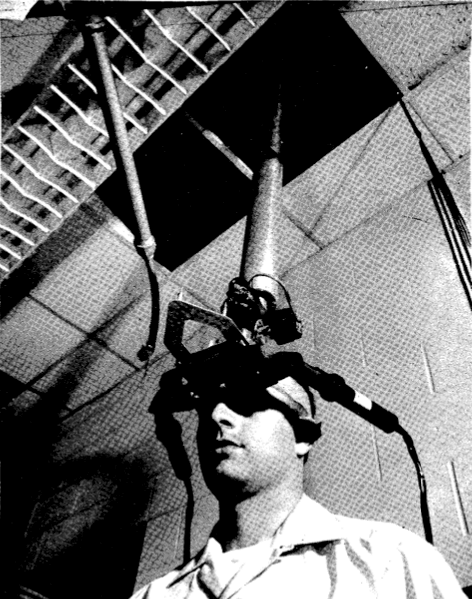
\includegraphics[width=.45\linewidth]{02-review/sutherland68_2.png}}
    \caption[Sutherland's `Ultimate Display']{Sutherland's `Ultimate Display'}\label{fig: sutherlandsword}
\end{figure}

Over the course of the proceeding thirty years, most display (visual, audio and haptic) technologies gained higher resolutions, whilst becoming ever more miniaturised, propelled by the general movement towards ubiquitous and wearable computing.  In 1992, augmented reality (AR) was officially defined by Boeing engineers Thomas Caudell and David Mizell, as a technology that could be used to `augment the visual field of the user with information' \citeyearpar{caudell1992}. Their prototype device featured display and tracking technologies built on the work of Sutherland. The purpose of the Caudell and Mizell’s device was to increase manufacture workers' efficiency through overlay of graphical wire-frame instructions. Their device operated by tracking elements of the users environment and body, processing these in real-time, and then overlaying these instructions in the appropriate places dependent on the manufacturing process through a HUDset. The HUDset, commonly referred to today as a head-mounted display (HMD) operated by updating the displays output in real-time dependent on the position and orientation (pose) of the participant. This had the effect of the graphical overlay seeming `fixed', or what is referred to now as `registered' or `aligned', on top of a specific point in the real world. For Caudell and Mizell, this display and tracking solution is what leads to the `technology' of AR being possible, and for them, it is what enables the context-aware instructional overlay of their application.

\begin{figure}[bth]
    \myfloatalign
    {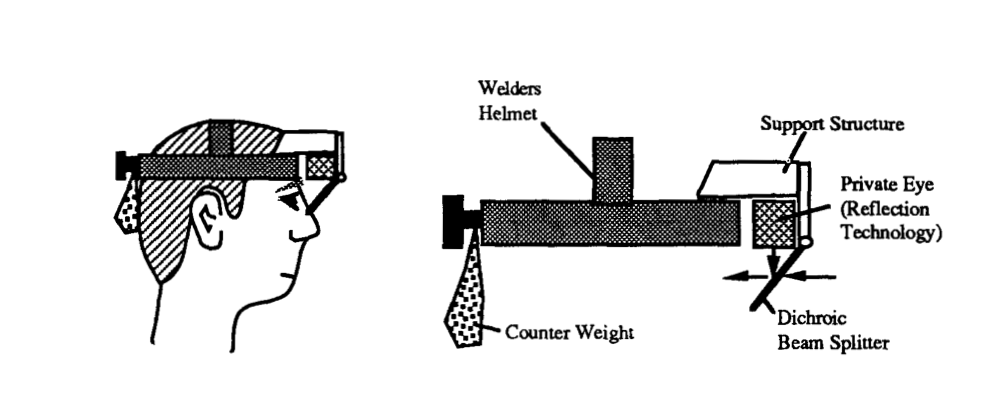
\includegraphics[width=0.75\linewidth]{02-review/caudell92_1.png}}
    \caption[Caudell and Mizell's device]{Caudell and Mizell's device}\label{fig: caudellprivateeye}
\end{figure}

Shortly after this original definition, Milgram and Kishino conceptualised the `Reality-Virtuality Continuum \citeyearpar{milgram1994}, which aimed to consolidate similar efforts across disciplines that were aiming to augment or virtualise `reality'. The continuum (\autoref{fig: milgramcontinuum}) defines two outer bounds of `Real Environments' on the left (which exist as physical and tangible matter), and `Virtual Environments' on the right (that exist solely as digital bits), and everything within was to be classed as `Mixed Reality' (MR). Within MR, use-cases closer to the `Real' were regarded as `Augmented Reality' (AR), and use-cases closer to the `Virtual', were regarded as `Augmented Virtuality' (AV). In separating these MR use-cases from the tele-robotics field of Virtual Reality / Virtual Environments (VR / VE), they proposed a clear framework for classifying works. Since both AR and AV make use of augmenting `by means of real objects' in today's use cases, (e.g. by tracking and parameterising hand gestures, or tracking and generating spatial maps of the real environment), the difference between AR and AV in this definition, problematically, becomes the `primary world' in which objects are are doing the augmenting. Indeed, Milgram and Kishino make note of the possibility of this in their paper: 

\begin{figure}[bth]
    \myfloatalign
    {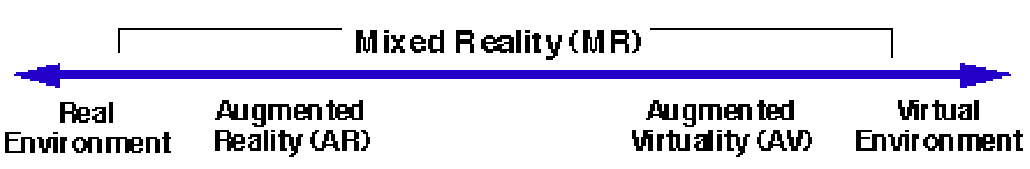
\includegraphics[width=0.75\linewidth]{02-review/milgram94_1.png}}
    \caption[`Reality - Virtuality Continuum']{`Reality - Virtuality Continuum'}\label{fig: milgramcontinuum}
\end{figure}

`Of course, as technology progresses, it may eventually become less straightforward to perceive whether the primary world being experienced is in fact predominantly `real' or predominantly `virtual', which may ultimately weaken the case for use of both AR and AV terms'

They further specify that, despite this is the case, it should not affect the validity of the more general [Mixed Reality] term to cover the `grey area' in the centre of the virtuality continuum, and also offer the term `Hybrid Reality' for displays that blend AR and AV compositely. Today, term `Mixed Reality' is seen seldom apart from its use within Microsoft's toolkit, and `Hybrid Reality' even less so. Therefore, as previously mentioned, due to the rapid evolution of these technologies, the present thesis makes no distinction between Mixed, Hybrid, and Augmented Reality.

In 1997, Azuma proposed a specification for the definition of an AR system, and surveyed the five years of AR research since Caudell and Mizell's original definition. In order to avoid limiting AR to specific technologies, they define AR as a `system' that follows three characteristics: 

\begin{itemize}
    \item Combines real and virtual
    \item Interactive in real time
    \item Registered in 3-D
\end{itemize}

In this paper, he distinguishes between optical and video based approaches to AR and while both of these methods can and had been realised (when speaking strictly of visual display of information) via head mounted display technologies, Azuma makes further room in the definition for monitor based approaches too, allowing the definition to be broad enough to encompass a variety of AR use cases, methods and processes. Not soon after, Azuma et al., classify three categories of `display': head worn, handheld and projective. For this reason, as well as the specification of three precise characteristics, Azuma’s definition of AR has become widespread. 

These early definitions and conceptions of AR were typically built upon with applications involving display and tracking technology that resulted in the \textbf{visual overlay and alignment} of \textbf{virtual graphics} onto our \textbf{real world environment}. Whilst this view of AR is followed by the overwhelming majority of historical and contemporary uses of AR, it only makes up a small subset of the potential myriad interactions afforded by the technologies that enable AR. Sutherland, who arguably catalysed early practical research in this field, viewed this AR as a `window' interface, that could serve `as many senses as possible'. Rosenberg, another early proponent of AR, developed the concept of `Virtual Fixtures' (overlaid sensory information) as a method of reducing the `tax' on our senses induced by an overload of information through the visual sense \citep{rosenberg1993}. Milgram and Kishino, in outlining their taxonomy, recognise that it could serve to alleviate `analogous issues associated with other display modalities`, and cite work from Cohen, who at the time was developing realistic acoustic environment rendering in AR \citeyearpar{cohen1993}. They also note the concurrent work in haptic (the various senses of touch) displays for augmented reality. 

Mann terms `Mediated Reality' \citeyearpar{mann1994} as more of a method to computationally mediate our own perception, rather than just focusing on overlaying. His later work terms `All Reality (*R)' which broadens the taxonomy of AR with concepts such as as surveillance and privacy \citeyearpar{mann2018}. Azuma et al., acknowledge that AR is not just limited to visual perception or overlaying processes: `AR can potentially apply to all senses, including hearing, touch, and smell. Certain AR applications also require removing real objects from the perceived environment, in addition to adding virtual objects'. With this in mind, what does the landscape of more contemporary AR design look and feel like today?


%*[ ]   fix width
\section{Forms of AR}\label{sec: ar-forms}
\subsection{Head-mounted}\label{sec: ar-forms-hmd}
\begin{figure}
    \centering
    \subcaptionbox{Sutherlands `Ultimate Display'\label{fig: historicalHMDs-sutherland}}[.3\linewidth]{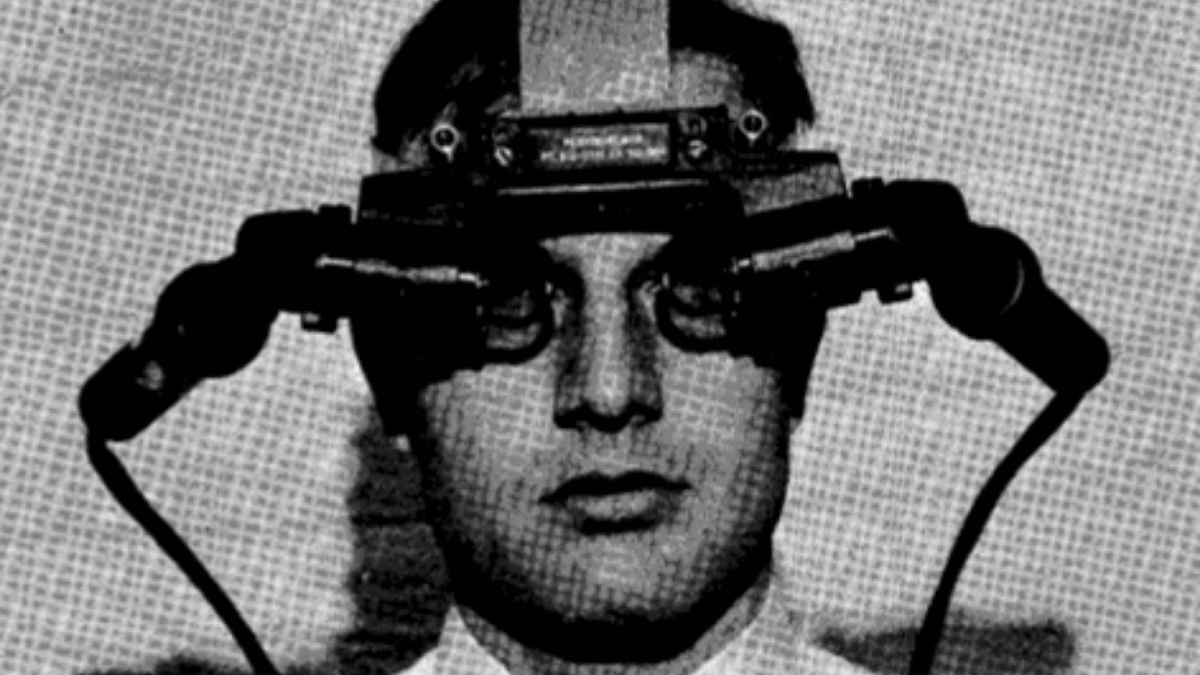
\includegraphics[height=2.5cm]{02-review/sutherland68_1.png}}
    \hfill
    \subcaptionbox{Caudell and Mizell's `HUDset'\label{fig: historicalHMDs-caudell}}[.3\linewidth]{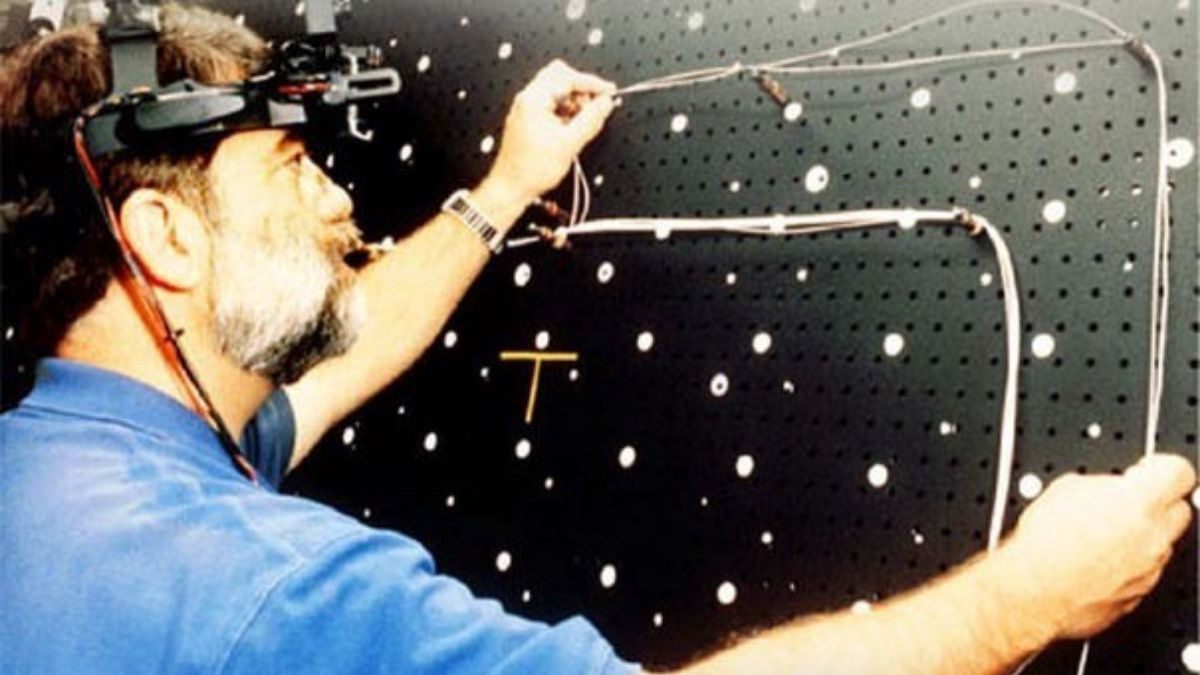
\includegraphics[height=2.5cm]{02-review/caudell92_2.jpeg}}
    \hfill
    \subcaptionbox{Feiner's `KARMA' System\label{fig: historicalHMDs-feiner}}[.3\linewidth]{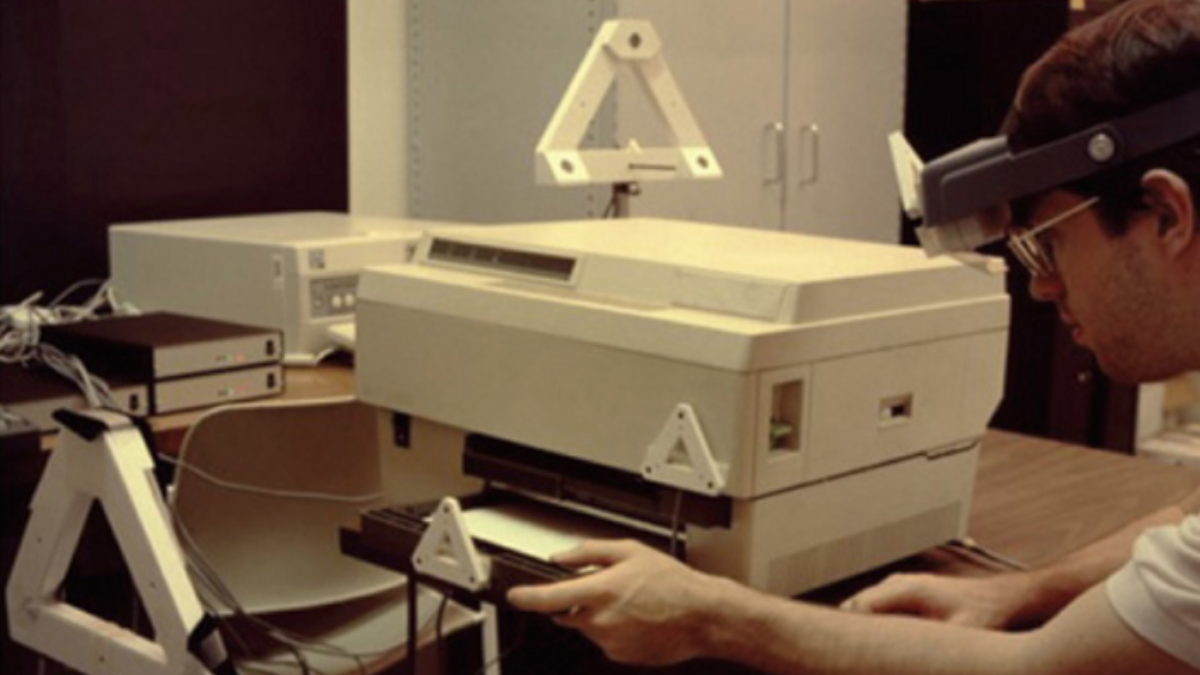
\includegraphics[height=2.5cm]{02-review/feiner93_1.png}}%
    \caption{Historical AR HMDs}
    \label{fig: historicalHMDs}
\end{figure}

Successors of AR head-mounted displays (HMDs) devised by Sutherland \citeyearpar{sutherland1968}, Caudell and Mizell \citeyearpar{caudell1992}, and Feiner \citeyearpar{feiner1993,feiner1997} exist today commercially within products such as the Microsoft Hololens 2 \footnote{\url{https://www.microsoft.com/en-us/hololens}}, the Magic Leap ML-1 \footnote{\url{https://www.magicleap.com/magic-leap-1}}, and the nReal Light \footnote{\url{https://nreal.ai/product/}}. These devices afford optical see-through capabilities through half-mirror visors and high-resolution displays, and offer stereo audio output. Input is managed mainly by hand-tracked interaction with overlaid visual menus and objects, but is also possible through eye tracking and voice control. The environment is sensed through a combination of 6DoF pose tracking, and spatial mesh mapping. For most HMDs today, this input and environment processing occurs off-device, on a tethered or wearable computer, or mobile device. These devices tend to be relatively expensive due to the extremely high R\&D costs associated with the field (due to its novelty). Leap Motion's open-source Project North Star \footnote{\url{https://docs.projectnorthstar.org/}} provides a much cheaper alternative at the trade-off of slightly larger form and lack of integrated computing and audio implementation, but has the highest field-of-view of all four and comparable tracking.

%*[ ]   fix figure
\begin{figure}
    \centering
    \subcaptionbox{Microsoft Hololens 2\label{fig: contemporaryHMDs-microsoft}}{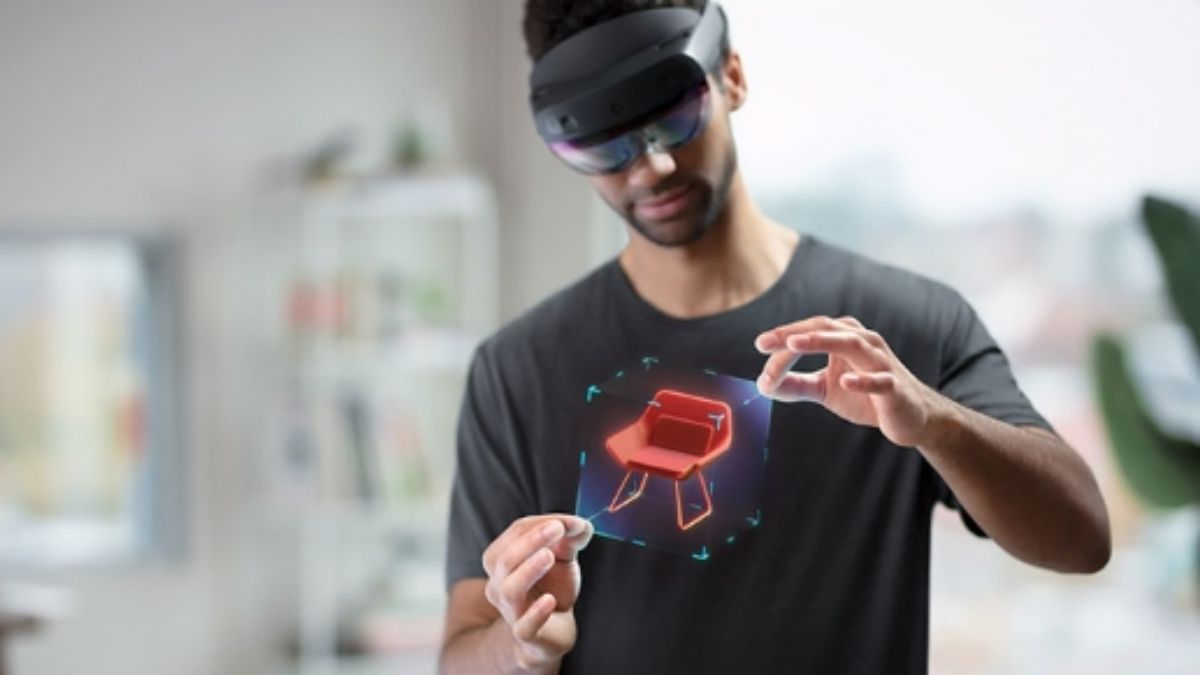
\includegraphics[width=0.45\linewidth]{02-review/hololens.jpg}}\quad
    \hfill
    \subcaptionbox{Magic Leap ML-1\label{fig: contemporaryHMDs-magicleap}}{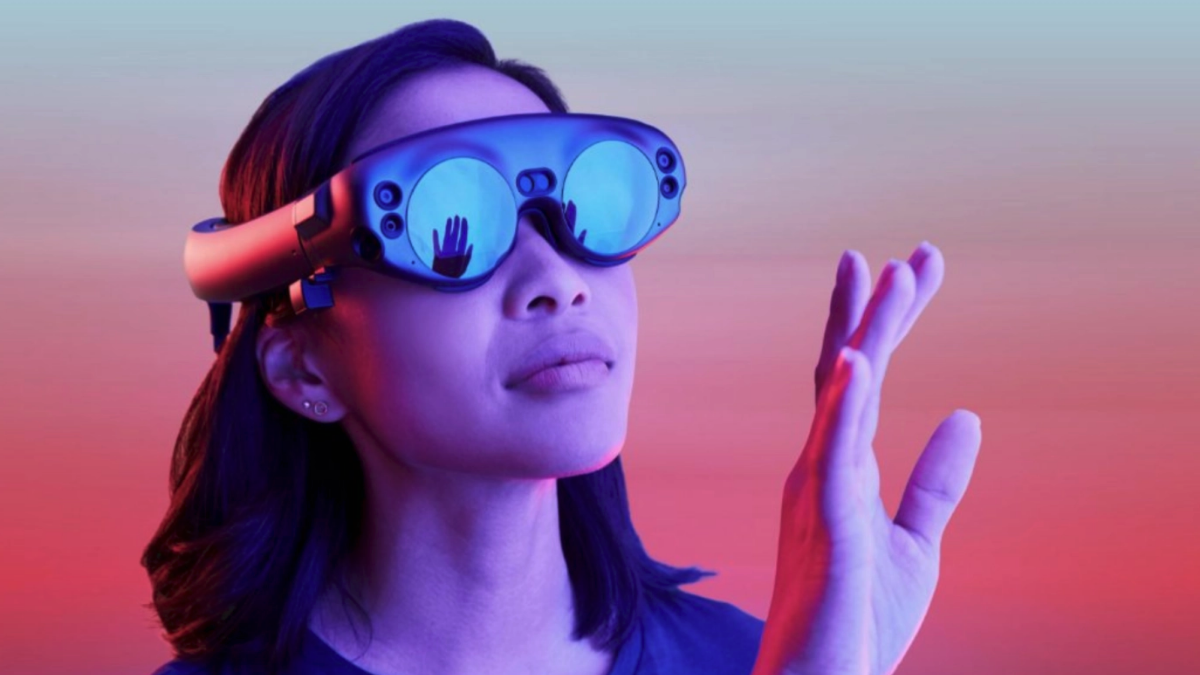
\includegraphics[width=0.45\linewidth]{02-review/magicleap.png}}\\
    \vspace{0.5cm}
    \subcaptionbox{nReal Light\label{fig: contemporaryHMDs-nreal}}{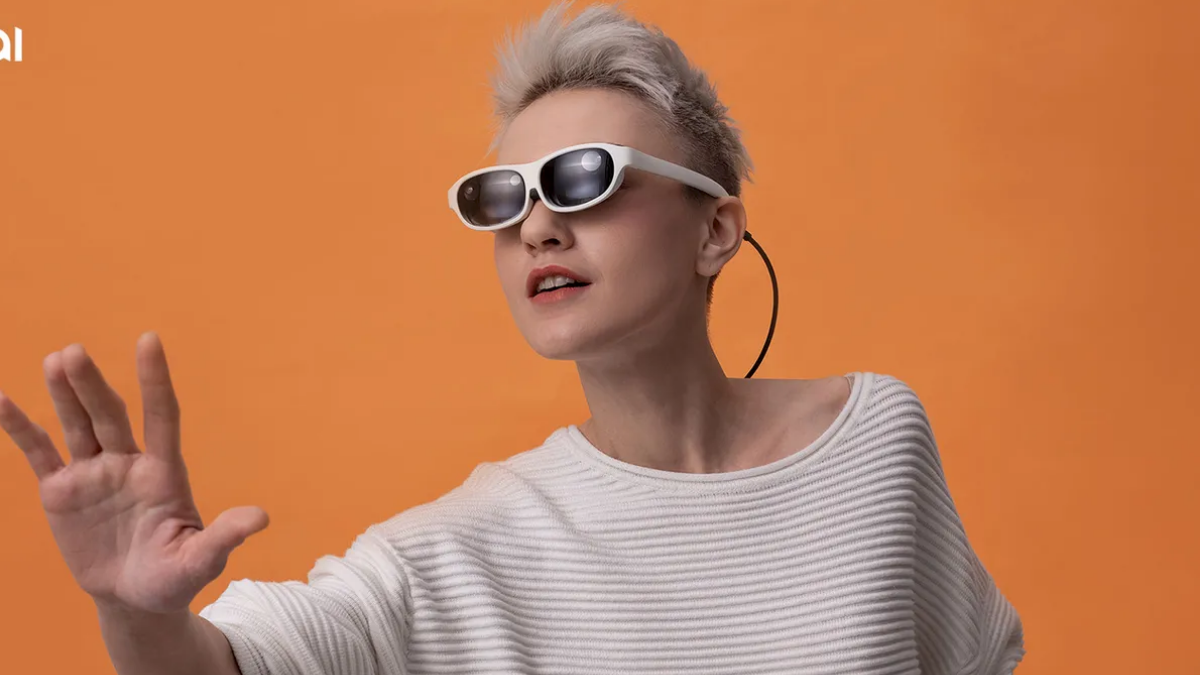
\includegraphics[width=0.45\linewidth]{02-review/nreal.png}}\quad
    \hfill
    \subcaptionbox{Leap Motion Project North Star\label{fig: contemporaryHMDs-northstar}}{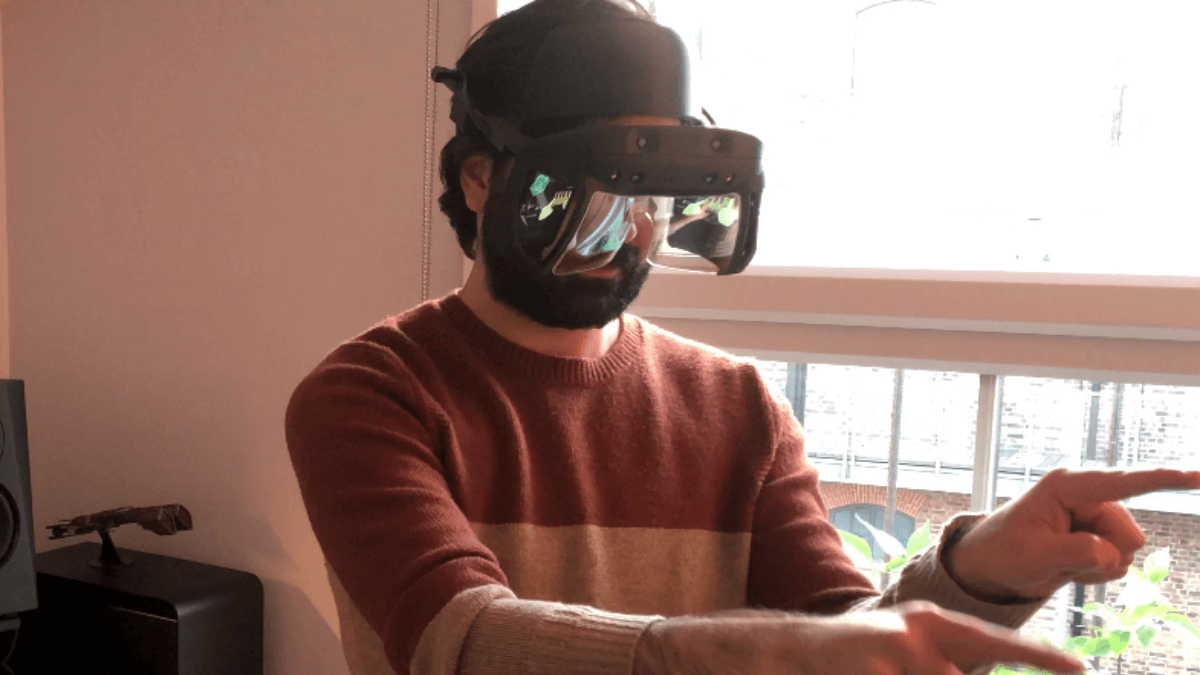
\includegraphics[width=0.45\linewidth]{02-review/northstar.png}}\\
    \caption{Contemporary AR HMDs}
    \label{fig: contemporaryHMDs}
\end{figure}

A device that is head-mounted poses clear benefits to both input and output modalities. For input sensors, being mounted on the head provides them with more accurate tracking from the perspectives of our own senses (organic sensors).  Consequently, and as Lindeman and Noma maintain in their classification scheme for multisensory AR, an important factor for the parity (if desired) of real and virtual output is a consideration of the location along the `stimulus pathway' at which they mix: at the environment, sensory subsystem or computer level \citeyearpar{lindeman2007}. For a device to be head-mounted, allows `mixing' to happen closer to the sensory subsystems, i.e. our eyes, ears, nose and mouth, thus resulting in an experience that is more closely intertwined with our real-time environment stimuli.

\subsection{Handheld}\label{sec: ar-forms-mobile}
Today, anyone who owns a smartphone is carrying an AR device in their pocket. This particular genre of AR development began in earnest in the mid 2000's and today is the most widely used form of AR due to the pervasiveness of smartphones. It builds on the early research and practice of handheld AR applications built on cellphones and personal digital assistants (PDAs) in the late 1990's, and smartphones in the late 2000’s, whose increasing variety and accuracy of onboard sensors: cameras, gyroscopes, accelerometers, and GPS, provided a convenient all-in-one solutions for developing handheld visual AR experiences. 

The limitations of handheld displays are outlined by Bimber and Raskar \citeyearpar[pp. 79-83]{bimber2005}: reduced immersiveness due to the small screen size, compounded by the distance between it and the participant (normally arms length), impaired gestural input due to the need to hold the device; restrictions due to the cameras image quality and less computational power available to effectively register (align) real and virtual objects. As well as these issues, smartphones have developed to be primarily visual devices despite their name, and as such, their ability to deliver high fidelity audio, let alone audio AR mixing is limited due to their distance from the ear. 

Recently, the lack of non-visual AR in handheld smartphones has been addressed through the increased adoption of `hearables', a marketing term for small and unobtrusive, wireless earphones. More specifically, two features make these suitable audio solutions for AR use; `transparent' hearing modes (see mic-through \citep{lindeman2008}), and integrated 6DoF \footnote{\url{https://www.apple.com/airpods-pro/specs/}}.

\subsection{Projective}\label{sec: ar-forms-proj}
Projection of data into the environment in order to overlay or alter perception of real objects, i.e mixing virtual and real stimuli at the environment level \citep{lindeman2007}, is perhaps the least adopted of Azuma's categories of AR. The property that sets projective AR apart from head-mounted and handheld AR is perhaps its potential to deliver experience to multiple participants within a space. Although collaboration is possible through the previous two categories, it requires all participants to engage technology that is affixed to their body (either through wearing or through holding). Projective AR alleviates both the burden of physical attachment to a device, and also the expense of procuring a device for each participant. This category of display is typically realised by use of video projectors and speakers. Although the base requirement of registration in three-dimensions between virtual and real (Azuma's third specification), is fulfilled relatively easily (add more projectors) compared to head-worn and handheld approaches (more sensor computation and accuracy), 

\subsection{Other forms}\label{sec: ar-forms-other}
Of course, this categorisation is not exhaustive, and leaves out body worn AR systems such as the Audiomented Sound System \citep{chevalier2020}, and tangible augmented objects \citep{schraffenberger2015}. This will be expanded on within my own framework towards designing multisensory AR instruments.
\section{Sensory Display in AR}\label{sec: ar-sensory}
Within these common forms of AR technology, one could split the various technological processes that occur into input, process, output (the general IPO model found in software engineering), in AR this is often labelled: tracking, process, display. Tracking, as mentioned is often through hand gesture, body position and orientation and voice activation. Display is managed in the majority of cases through screens. The present section outlines various other sensory displays that have the potential of creating more immersive tools of expression.

\subsection{Visual Sense}\label{sec: ar-sensory-visual}
It is poignant to mention that until that last 20 years or so, sensory sciences, and as a result, technological displays of information, were focused on the visual, with the auditory following behind, and then the touch, smell and taste senses. In cross-modality psychology research, this ocularcentrism (the perceptual and epistemological bias ranking vision over other senses) is normally explained by a `textbook' explanation: `the idea that vision is the most important modality is supported by numerous studies demonstrating visual dominance.' Fabian Hutmacher argues that ocularcentrism can be critiqued through the lenses of \citeyearpar{hutmacher2019}: 

\begin{itemize}
    \item A methodological-structural explanation: `Research on vision is often easier than research on other modalities and that this is the result of an initial bias toward vision that reinforces itself.'
    \item A cultural explanation: `The dominance of the visual is not a historical constant, but rather a result of the way (Western) societies are designed.'
\end{itemize}

However, AR is still typically realised in the form of graphical overlay, and as such, the forms which we find ourselves interacting with are predominantly based around screens and other forms of visual display \citep{dey2018}. These are often split into optical and video see-through methods of display. The former employs semi-reflective half-mirrors to combine the reflection of close-by screen with the natural pass-through of the real world; the latter uses the feed of cameras to completely occlude the participant's vision, and performs AR processes on top of the camera feed. There are advantages and disadvantages to both methods, outlined in \citep{rolland2000}. Head-mounted systems tend towards optical see-through, whereas most handheld AR (smartphones) are exhibit video see-through AR.

\subsection{Auditory Sense}\label{sec: ar-sensory-auditory}
The second most developed-for sense in AR is the auditory system, borrowing from a rich history of spatial audio techniques such as exploiting HRTF for binaural audio playback and realistic audio localisation. Within the field of audio AR, as previously mentioned, `hearables' with `transparency hearing` modes offer the auditory equivalent of video see-through (coined mic-through \citep{lindeman2008}), where the occluded outside world is captured through a microphone, on top of which virtual sounds can be processed. Also outlined by Lindeman and Noma is the use of bone conduction headphones to offer a mediated perception of sound environments without the need to occlude the participants ears (coined hear-through), which could be considered equivalent to optical see-through. Moving into the environment, there are a myriad spatial audio techniques that could be used within AR, delivered by speaker arrays such as those found in wave-field synthesis and ambisonic beam-forming practices.

\subsection{Haptic Sense}\label{sec: ar-sensory-haptic}
Due to the prevalence of hand-tracking technologies in the interaction with head-mounted AR applications, one might assume that being able to actually \textit{feel} the virtual objects that are placed in AR would be one of the most important and developed concepts in AR. However, much of the early research in AR placed importance around overlaying instructions, rather than interactive objects. Hence, the haptic feedback of touching AR objects is relatively under-explored compared to the common issues which affected early and (funded) research - accurate registration of real and virtual processes; and higher visual fidelity. In most cases, it was deemed enough to \textit{see} the effect that ones hands or body position had on the AR object or scene respectively. Today, there exist numerous technologies that could provide computationally mediated haptic perception in AR, for example through vibrotactile feedback or electrical muscle stimulation \citep{lopes2018}.

\subsection{The Chemical Senses}\label{sec: ar-sensory-chemical}
Whereas auditory and haptic sensations have been developed in AR, the chemical senses (smell and taste) have received far less exploration. Visual, auditory, and touch information can be believably recreated with technology through analog to digital conversion of electromagnetic radiation (light) and mechanical wave transmission (sound and touch). Conversely, smells and tastes contain organic information, the sensors (and thus A2D conversion) for which have not been invented yet. As such, the closest we can get to receiving chemical sensory data is through computationally activated rather than computationally mediated displays: scent emitters \citep{maggioni2019}, and taste patches for example. Accordingly, in order to mediate the sense of taste, creative methods of sensory illusion have often been employed, i.e. Narumi et al. demonstrating that the sense of flavour can be mediated via visual overlay in AR \citep{narumi2011}. The sense of temperature has also been mediated through cross-modal sensory illusion exploiting the trigeminal nerve in the nose, Brooks et al. demonstrates that users in VR can be made to feel warmer or colder based on the relative amounts of capsaicin or eucalyptus emitted near the nose \citeyearpar{brooks2020}.
\section{Processes in AR}\label{sec: ar-process}
Additive layering of virtual content onto our real environment is by far the most typical of processes experienced in AR. However, it is only one of the potential methods of interaction between virtual and real components. In navigating this issue, the present thesis aligns its conception of AR closely with the definition of AR by Chevalier and Kiefer \citeyearpar{chevalier2020}: `real-time computationally mediated perception', which fulfils Azuma's three characteristics of AR systems, but is not as exclusionary as Caudell and Mizell's original definition: a technology used to  `augment the visual field of the user with information'. Investigating the existing relationships between real and virtual components of AR systems, Schraffenberger outlines at least five `relationships' and five `subforms' of AR (see \autoref{table:schraffenbergertaxonomy}). This taxonomy \citeyearpar[pp. 80-130]{schraffenberger2018} provides an ideal starting point for those designing AR systems interested in creating embodied experiences that challenge the typicality of basic visual-overlay AR. Furthermore, Mann expands the `Reality - Virtuality Continuum' \citep{milgram1994} into the `All Reality Continuum', integrating further dimensions such as `Metaveillance', `Kineveillance' and `Phenomenality', such a standpoint not only `anticipates the need for an ethically aligned reality' \citeyearpar{mann2018}, but demonstrates the multifaceted nature of augmented reality to afford experiences of ourselves, others, and environments computationally mediated by more than just additive informational overlays.

\begin{table}
    \centering
    \begin{tabular}{ l l }
        \toprule
        Relationship        & Description                       \\
        \midrule
        Coexistence         & Unrelated                         \\
        Presence            & Spatially Related                 \\
        Information         & Content-Based Relationship        \\
        Physical            & Affect Each Other                 \\
        Behavioural         & Sense and React to Each Other     \\
        \midrule
        \midrule
        Subform             & Description                       \\
        \midrule
        Extended Reality    & The Virtual Supplements the Real  \\
        Diminished Reality  & The Virtual Removes the Real      \\
        Altered Reality     & The Virtual Transforms the Real   \\
        Hybrid Reality      & The Virtual Completes the Real    \\
        Extended Perception & Translating the Inperceptible     \\
        \bottomrule
    \end{tabular}
    \caption{Schraffenberger's taxonomy of relationships and emergent AR subforms}\label{table:schraffenbergertaxonomy}
\end{table}

In particular, `diminished reality', aims to \textit{remove} real objects in our environment. When explored in the visual sense, this approach uses computer vision and content-aware substitution to remove a section or object of the real-world environment through camera sensors. Noise cancelling potentially offers an auditory diminished reality, but due to the fact that sound is propagated via mechanical waves, our sense of sound is closely intertwined with physically feelings of vibration, which are much harder to remove \citep{mori2017}. Further examples of sound-driven but cross-modal techniques are outlined in \citep{walther-hansen2020}.

`Altered reality' has the potential to provide new and otherwise inaccessible sensory and perceptual experience Schraffenberger describes that this is possible through virtual components altering the perception of real components in an AR system. Mann outlines a myriad examples of altered visual percepts \citeyearpar{mann1994}, from giants eyes, to `slow' glasses. More recently, Nishida et al. have experimented with `egocentric smaller-person experience' through use of a video see-through AR headset, in which unlike typical AR, the cameras are mounted at waist height, rather than on the HMD \citeyearpar{nishida2019}. This afforded participants a difference in real-time visual perception, and resulted in them generally feeling smaller and behaving more like a child. In tandem with this altered visual perception, they propose a modified robotic glove `HandMorph' \citeyearpar{nishida2020} that alters sensations of touch through reduced finger and overall grip size. 

\begin{figure}[bth]
    \myfloatalign
    {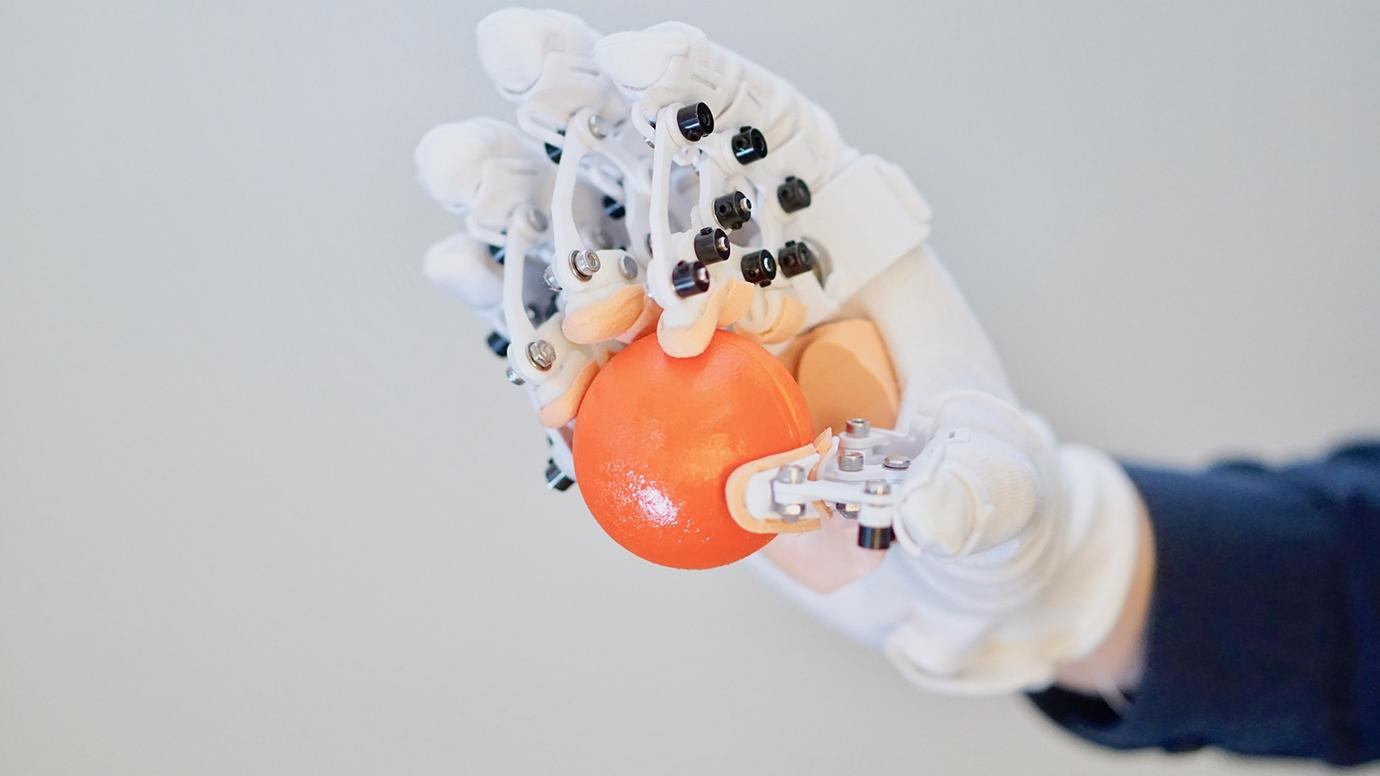
\includegraphics[width=.45\linewidth]{02-review/nishida20_1.jpg}}
    \caption[Nishida's `HandMorph']{Nishida's `HandMorph'}\label{fig: handmorph}
\end{figure}

In a similar vein, `extended perception' revolves around the potential to provide \textit{more} senses, or the sensing of stimuli outside of the range of our sensory systems. Bees for example have a visual system that extends far further into the ultraviolet range of EM radiation than our own eyes allow us; dogs hear much higher frequencies our ears allow us (thank goodness); and sharks can smell one part blood in a million parts water. These fun facts demonstrate vast differences in sensory acuity between species; but did you know that some shark have a constellation of pores \footnote{\url{https://www.sharktrust.org/shark-senses}} along the lateral side of their bodies that allows them to perceive minute pressure changes in water? This enables them to create a `pressure map' of their surroundings through active body movement. Modern technology could endow us with similar and myriad extended perceptions of our environment and its stimuli; Mann has experimented with making representations of radio waves translated down to the sensory range of our own eyes \citeyearpar{mann2018a}

\begin{figure}[bth]
    \myfloatalign
    {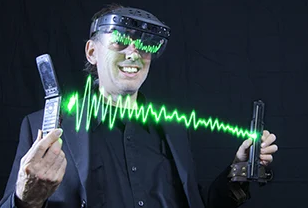
\includegraphics[width=.45\linewidth]{02-review/mann18_1.png}}
    \caption[Mann's `Sequential Wave Imprinting Machine']{Mann's `Sequential Wave Imprinting Machine'}\label{fig: mann_swim}
\end{figure}

 This section demonstrates the multitude of potential experiences that AR affords beyond mere visual information layering, next, I will examine the usage of AR in the arts, as a medium or tool for creating immersive aesthetic experiences, and demonstrate how this contributes towards a more holistic understanding of AR as a technology. 



% --------------------------------------------------------------------------- %
\section{Augmented Reality in the Arts}\label{sec: ar-arts}
Computational art, the use of computational programming or software as a tool, performance aid, medium or collaborator to create art or artistic works, is currently witnessing the adoption of new and exciting technologies such as trained machine learning algorithms, increasingly immersive displays and large-scale networked experiences. These implementations of technology within the creation artworks leads to a greater understanding of the materiality and affordance of these technologies. In this section, I draw attention the the modes of sensory engagment, aesthetic experience, collaborative expression, and activism that AR specifically affords artists willing to explioit its use as a medium.

\subsection{Sensory Engagement}\label{sec: ar-arts-sensory}
Computational art has seen the use of AR as a medium since the early 2000’s: in 2008, Grasset et al. presented case studies of AR art exhibitions, with the conclusion that for effective design of artworks, specific importance should be placed on the relationship \textit{between} real and virtual components \citeyearpar{grasset2008}. These relationships have come to describe a matrix of possibilities between senses and mediating processes, i.e. altered hearing, extended smell, diminished sight. Papagiannis has drawn attention to this broader multisensory view of AR in attempting to understand an aesthetic for AR applications, `AR is beginning to expand in new ways, beyond visual frames and into the full human sensorium' \citeyearpar{papagiannis2014}. In 2015, the Tate Sensorium multisensory art exhibition used novel mid-air haptic devices to augment visual art \citep{vi2017a}. The results of the included study found that more congruent multisensory experiences lead to audiences finding artwork more emotionally engaging. If more congruent multisensory experiences of art lead to more emotional engagement, and AR has the potential to mediate multiple senses in rich and provocative ways, surely this makes it an ideal medium for such works. 

\begin{figure}[bth]
    \myfloatalign
    {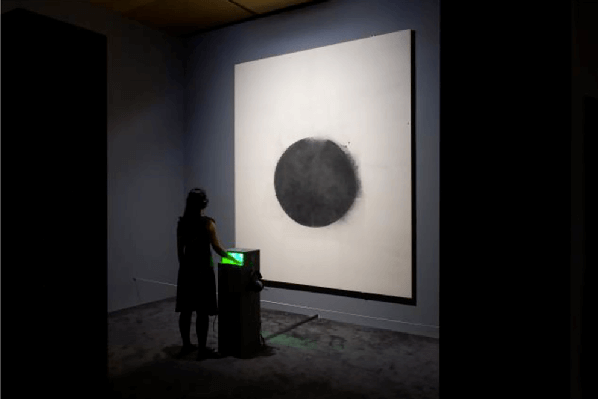
\includegraphics[width=.75\linewidth]{02-review/vi17_1.png}}
    \caption[Tate Sensorium Multisensory Art]{Tate Sensorium Multisensory Art}\label{fig: tate}
\end{figure}

\subsection{Aesthetic Experience}\label{sec: ar-arts-aesthetics}
Chevalier and Kiefer highlight the nascent use of newer AR technologies by artists \citeyearpar{chevalier2020}. They argue that AR has far more potential for creative exploration, and that it is a medium for creating `new nuanced and fine-grained emergent aesthetic experiences' and as previously mentioned, necessarily define AR as `real-time computationally mediated perception' in order to be inclusive of a multisensory approach to design. 

The installation `Concrete Storm'\footnote{\url{https://www.studiodrift.com/concrete-storm-microsoft}} by artists Gordijn and Nauta demonstrates the ability for AR to afford novel experiences of seemingly immutable and rigid physical objects (short concrete pillars), through the extension and animation of the concrete into larger, shifting and breaking structures. In describing the design of the work, they outline one of the main impetuses of creating the work: `Gordijn says the duo was interested in beginning to investigate the point at which viewers `might let go of trying to distinguish between what is real, what is not' and accept this new mixed world as simply another version of reality' \citep{gottschalk2017}. 

\begin{figure}[bth]
    \myfloatalign
    {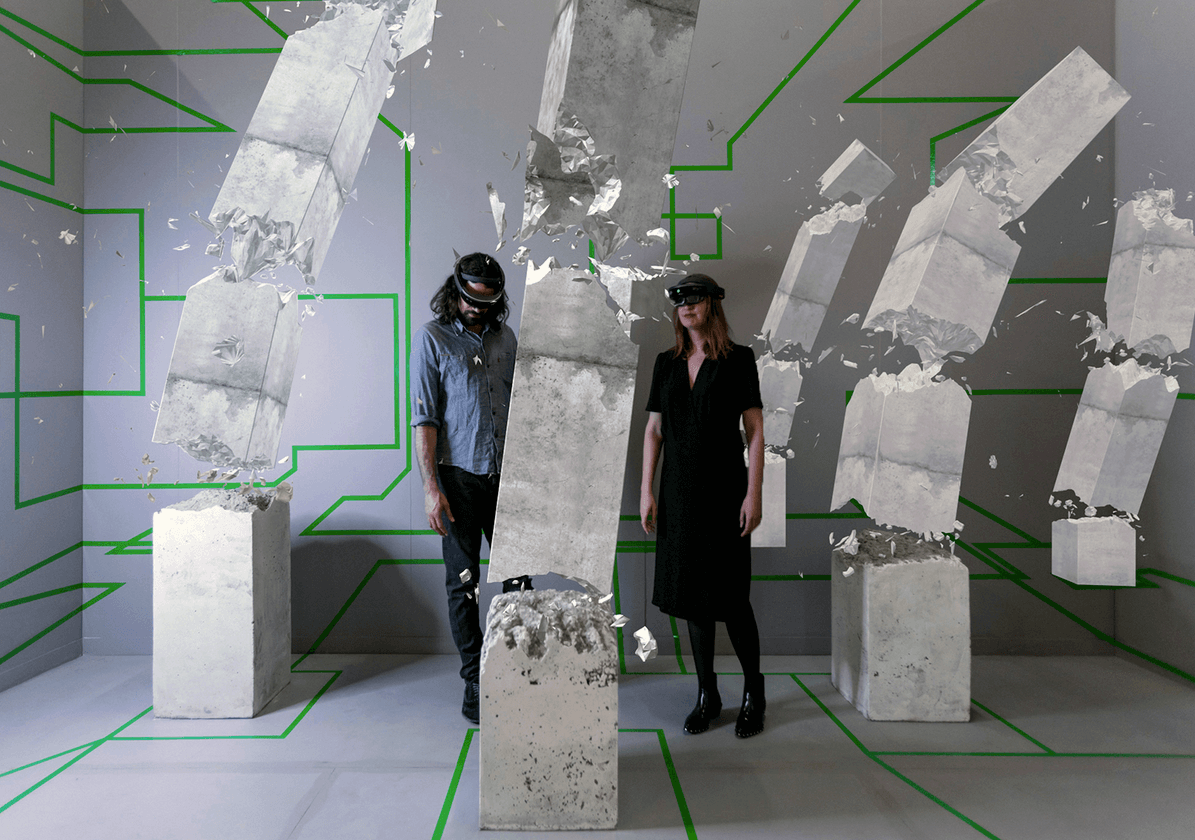
\includegraphics[width=.75\linewidth]{02-review/studiodrift.png}}
    \caption[Concrete Storm]{Concrete Storm}
\end{figure}\label{fig: concretestorm}

\subsection{Collaborative Expression}\label{sec: ar-arts-collaboration}
Another key aspect of the use of AR as a medium in computational artworks is its ability to enable collaborative expression and construct shared perceptual spaces. For example, Listening Mirrors\footnote{\url{http://listeningmirrors.net/}}, an artwork by Chevalier and Kiefer, \citeyearpar{chevalier2018} is an AR installation that engenders a collaborative and performative AR sound environment. This environment is hybrid in nature; split between physical and virtual space. In the installation space, participants can interact with a audio augmented parabolic acoustic mirror. Their interactions are intertwined with a computationally mediated virtual sonic environment that they experience through bone conduction headphones. Additionally their vocalisations are mediated by a wearable microphone through the mirror. This invites collaborative expression through exploration of the shared sonic world.

Similarly, Eno and Chilvers explore collaborative ambient audiovisual composition in their AR adaptation of the popular app `Bloom', `Bloom: Space' \footnote{\url{https://inculture.microsoft.com/musicxtech/bloom-open-space/}}. In this installation, participants wear a Microsoft Hololens and use hand gestures to activate and manipulate generative audiovisual elements. These elements can be experienced by other participants and thus create a shared perceptual and actionable space.

%*[ ]   fix figure
\begin{figure}
    \centering
    \subcaptionbox{Listening Mirrors\label{fig: collaborativeARt-listeningmirrors}}{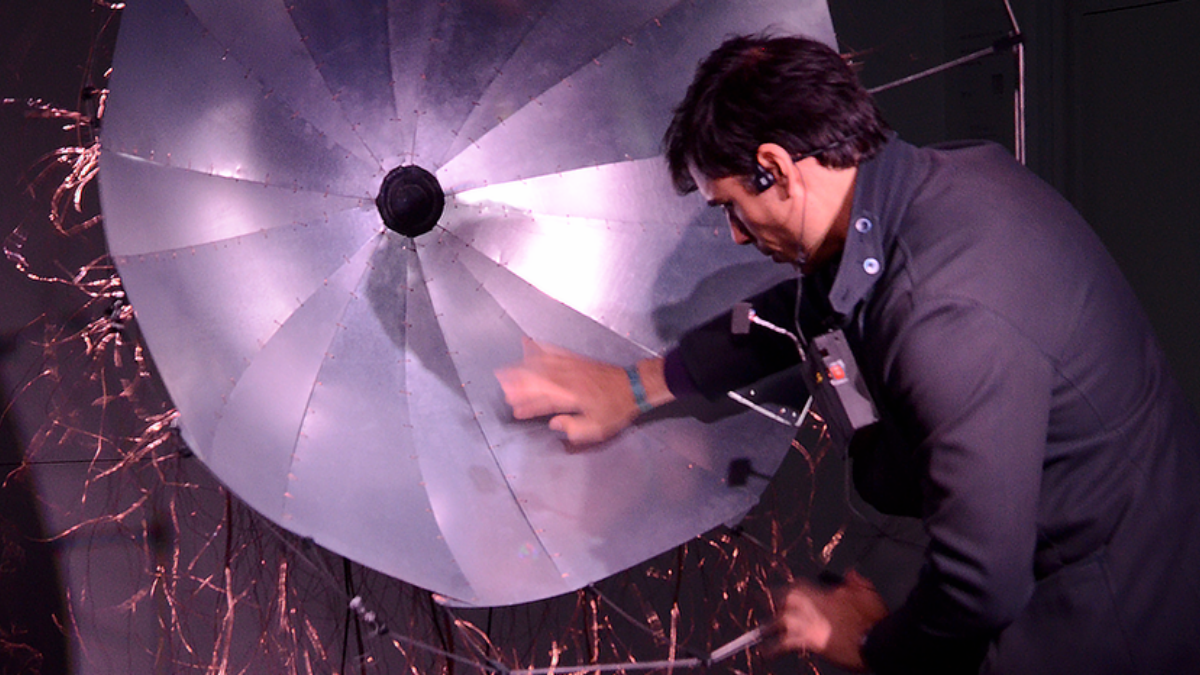
\includegraphics[width=0.45\linewidth]{02-review/chevalier18_1.png}}
    \hfill
    \subcaptionbox{Bloom: Space\label{fig: collaborativeARt-bloom}}{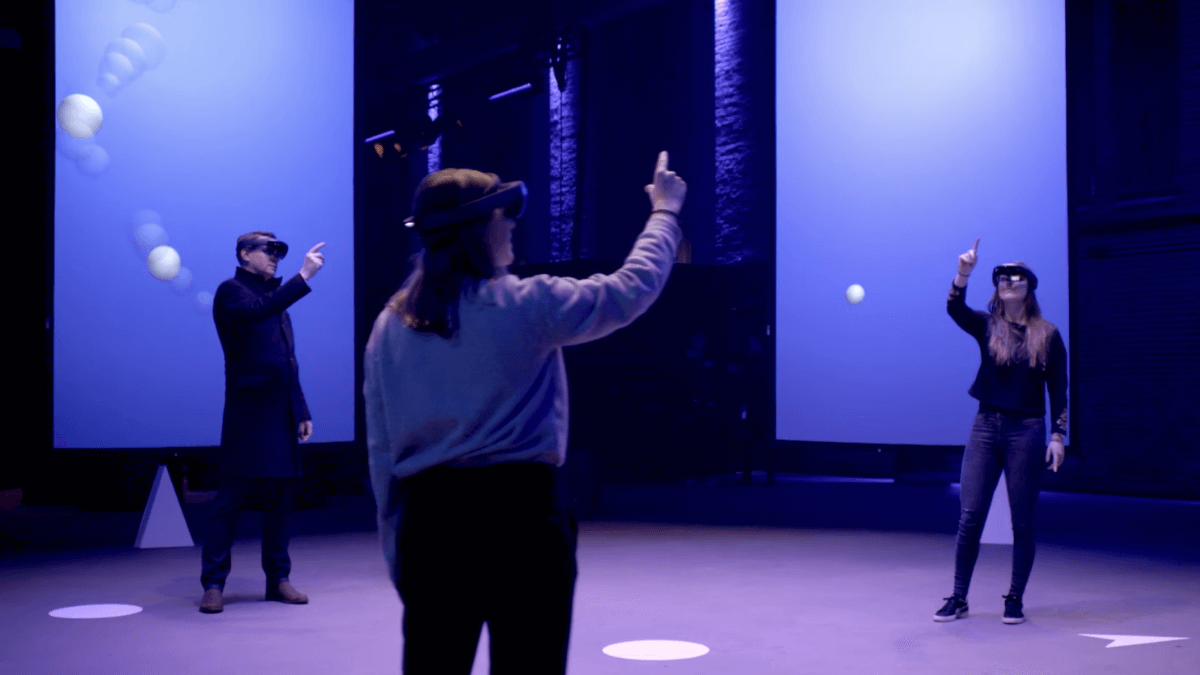
\includegraphics[width=0.45\linewidth]{02-review/bloom.png}}
    \caption{Collaborative Expression in AR}
    \label{fig: collaborativeARt}
\end{figure}

\subsection{Activism and Agency}\label{sec: ar-arts-activism}
Due to its ability to be an effective tool for collaborative expression, or perhaps because it creates a liminal hybridity that `questions the possession and control of a physical space' \citep{thiel2018}, AR art has seen use in activism and collaborative political expression. Early pioneers such as the Manifest.AR group were able to create convincing and socially immersive AR art using visual layering \footnote{\url{http://www.sndrv.nl/moma/}}. They did this through aligning the collaborative potential of AR with political expression. By creating an app that overlaid visual art within the Museum of Modern Art (MoMA) through GPS, they allowed participants to visit an exhibition in the museum that had not been organised by MoMA themselves (\autoref{fig: activismARt-moma}). AR thereby afforded these artists the ability to embed virtual art within an area considered private property, and also promote collective AR agency, raising very early questions about `virtual trespass' with AR. In a similar vein, `\#arOCCUPYWALLSTREET' (\#arOWS) was an arm of the Occupy Wall Street protests of 2011. Some 25 artists succeeded in overlaying the Wall Street area with `over 400 protest related augments', including audio overlays of protesters who were forbidden by police to enter the area. In this way, `AR was able to overcome their surveillance, barricades, horses, and excessive police numbers' \citeyearpar{skwarek2018} and more easily provide the means to action to people unable to physically mobilise.

As well as its liminality between real and virtual space promoting otherwise dangerous collaborative expression, AR has the power of rendering the invisible as seen, and due to this, it is a tool that has be used to shine light on social, economic, political and environmental injustices. Through its ability to change our perception of the real world through sensory augmentation, diminishment, hybridisation and extension, it has been used as a medium within the arts to `uncover' underlying mechanisms in our society. For example, Thiel and PATTU's (artists Cem Kozar and Işıl Ünal) 2011 work `Invisible Istanbul' aims to render visible the unseen urban dynamics of Istanbul, through GPS positioning smartphone visual overlay. They write: `Viewers become as photographers: the act of viewing or making a screenshot of the objects at a specific site and time reifies the virtual objects into artworks, revealing hidden forces within the city not visible to the naked eye.' \citeyearpar{thiel2011}. In PATTU's work, an augmented reality walking tour, different parts of the city are overlaid with symbolic information of past, present, and future uses of each area, highlighting tensions from military and commercial uses, and the effects this has on `contemporary urban space and the lives of its inhabitants' \citeyearpar{thiel2018}.

%*[ ]   fix figure
\begin{figure}
    \centering
    \subcaptionbox{Manifest.AR MoMA Invasion\label{fig: activismARt-moma}}{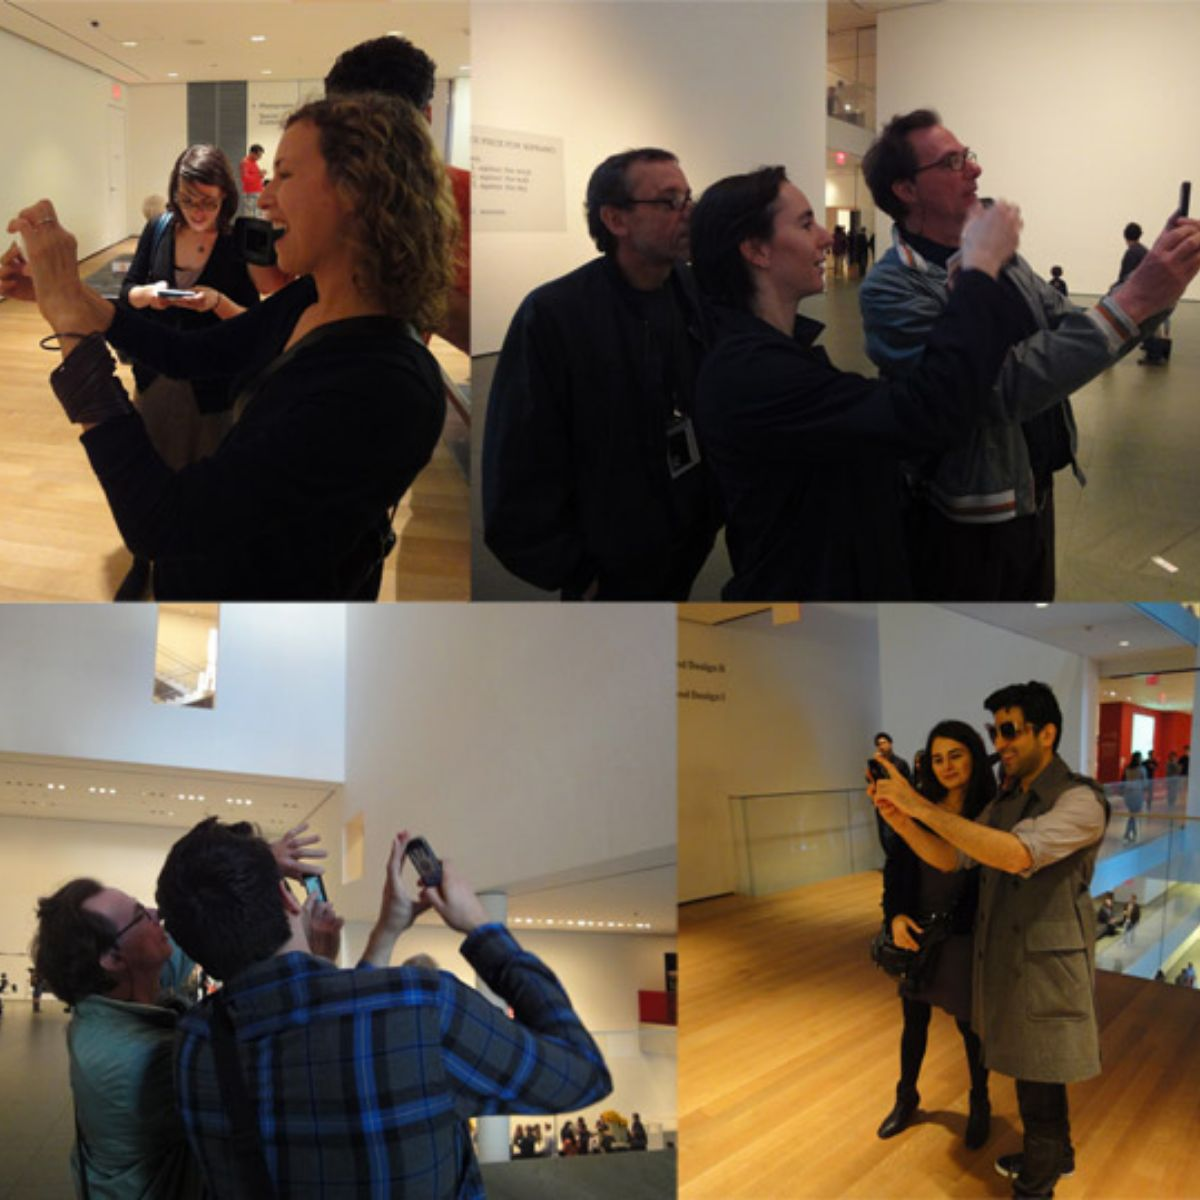
\includegraphics[width=0.45\linewidth]{02-review/moma.jpg}}
    \subcaptionbox{Invisible Istanbul\label{fig: activismARt-istanbul}}{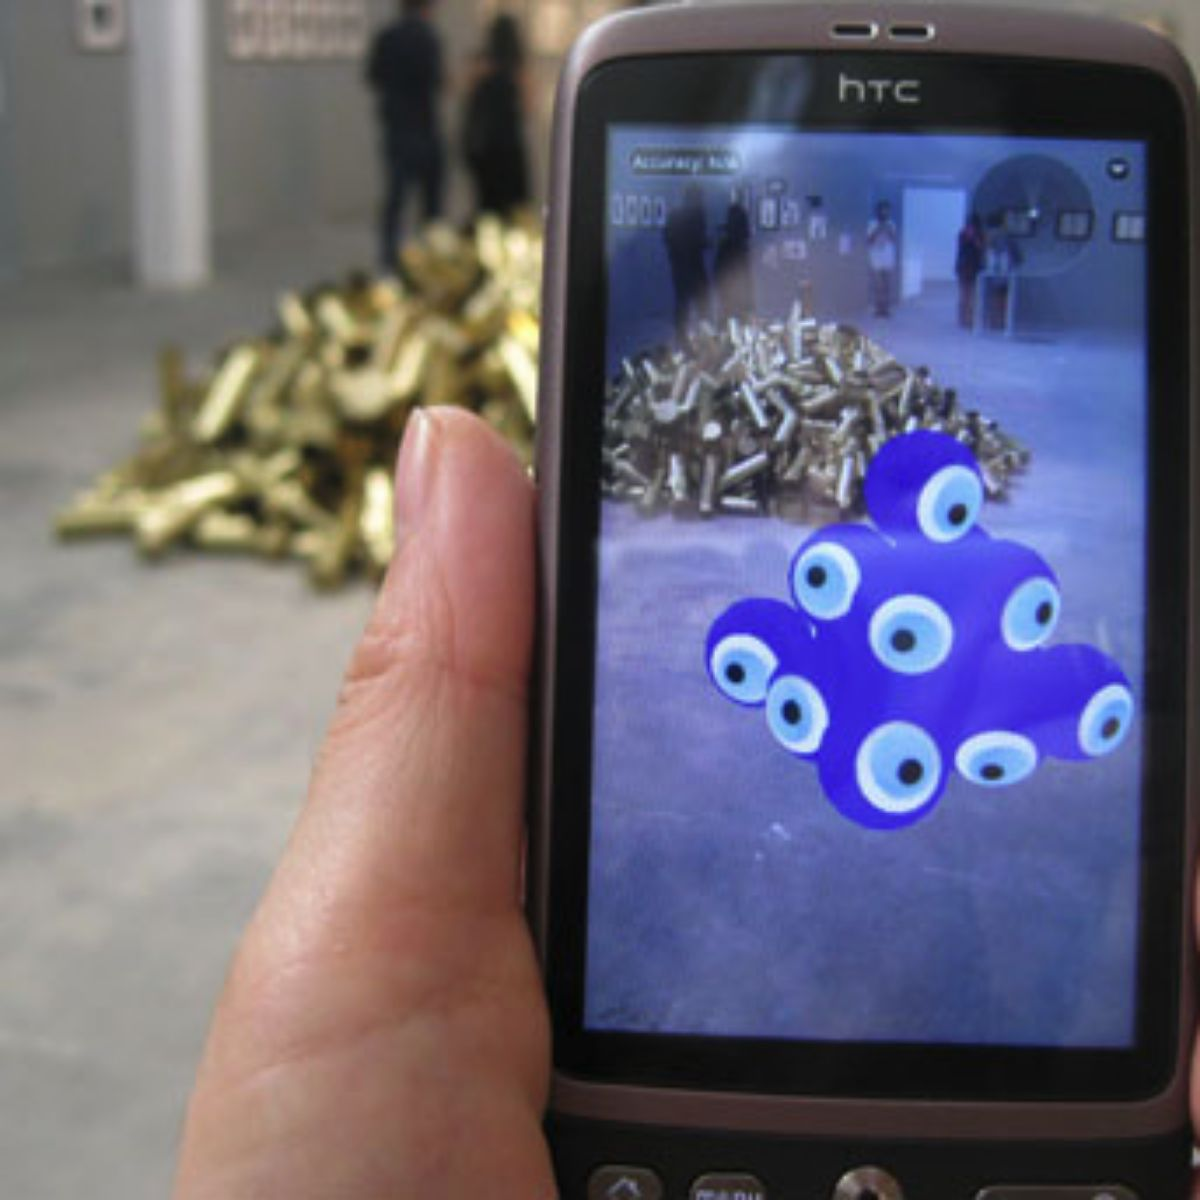
\includegraphics[width=0.45\linewidth]{02-review/thiel.jpg}}
    \caption{Activism through Interventionist ARt}
    \label{fig: activismARt}
\end{figure}


As summarised by Manifest.AR member Martin Skwarek puts it: `Alice has stepped through the looking glass [...] It is the job all future artists and activists to use this technology for the better, to bring people together, and uproot social injustice.' \citeyearpar{skwarek2018}



\subsection{Towards an Embodied Understanding of Musical AR Art}\label{sec: ar-arts-designingart}
Agreeing that AR can be used as a medium for the composition of computational art through software tool or instrument design, surfaces the question of what the materiality, both for user and developer, of such a digital tool, or piece software would look, sound, feel, taste or smell like. As Papagiannis highlights, `Understanding the capacities of the technology and its constraints to exploit the technology to artistic use by envisioning novel applications and approaches, and developing new aesthetics and conventions beyond previous traditional forms' \citeyearpar{papagiannis2017}.

If visual overlay AR has been used as `a viewing instrument to bring into focus forces invisible to the naked or unknowing eye, and make them visible in the public sphere.' \citep{thiel2011}, what emergent properties might devices rising out from multisensory approaches to design afford? What are the futures of digital musical instruments, whos designers opt to use this technology?


The next chapter explores three theoretical approaches that will help us further understand the \textit{materiality} afforded by AR when used as a medium for creative expression, the experience of \textit{embodiment} it has the potential of imparting on its immersants, and about the hybrid real-virtual \textit{space} it co-constructs with them when in use.

  \clearpage% --------------------------------------------------------------------------- %
%               _ _       _ _        _                       _                %
%            __| (_) __ _(_) |_ __ _| |  _ __ ___  _   _ ___(_) ___           %
%           / _` | |/ _` | | __/ _` | | | '_ ` _ \| | | / __| |/ __|          %
%          | (_| | | (_| | | || (_| | | | | | | | | |_| \__ \ | (__           %
%           \__,_|_|\__, |_|\__\__,_|_| |_| |_| |_|\__,_|___/_|\___|          %
%                   |___/                                                     %
%                                                                             %
%           _           _                                   _                 %
%          (_)_ __  ___| |_ _ __ _   _ _ __ ___   ___ _ __ | |_ ___           %
%          | | '_ \/ __| __| '__| | | | '_ ` _ \ / _ \ '_ \| __/ __|          %
%          | | | | \__ \ |_| |  | |_| | | | | | |  __/ | | | |_\__ \          %
%          |_|_| |_|___/\__|_|   \__,_|_| |_| |_|\___|_| |_|\__|___/          %
% --------------------------------------------------------------------------- %
\chapter{Aesthetic Experience, Complex Music Systems, and the Metaverse}
\label{sec: theory}
\epigraph{\emph{In actual experience, there is never any such isolated singular object or event; an object or event is always a special part, phase, or aspect, of an environing experienced world—a situation'}}{\citep[p. 67]{dewey1934}}

\begin{figure}
    \centering
    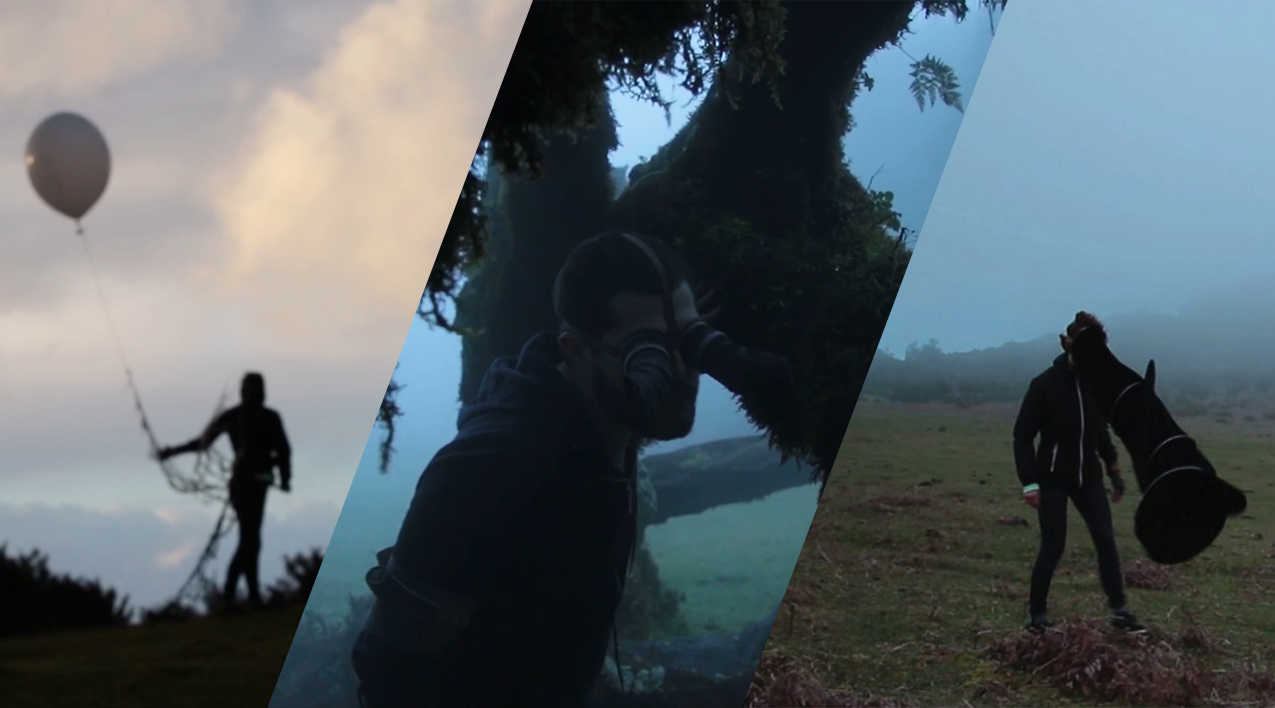
\includegraphics[width=1\linewidth]{03-theory/chapter-fig.png}
    \captionsetup{labelformat=empty}
    \caption[\autoref*{sec: theory}'s page-figure: Three photographs from the Sensory Cartographies project, (from \citefullauthor{tonn2017}, \citeyear{tonn2017})]{}
\end{figure}

\clearpage
% --------------------------------------------------------------------------- %
\section{Summary}\label{sec: theory-summary}
In the previous chapter, I outlined the problematic origins of \gls{ar} technology from within the U.S. \gls{mic}. This origination from within neo-colonial and capitalist modes of thought has had a compounded effect on the form that \gls{ar} takes today: predominantly it is sought as a `visual overlay' device. Despite this, clearly limiting perspective, we are seeing (or indeed hearing) increased use of \gls{ar} as a medium for the creation of meaningful experiences through interactive artwork. Though fairly established in modes of visual art because of this predominant form, its use in sound related art forms has been limited. As a result, the present thesis promotes a sensory-process agnostic \footnote{That is to say, not limited to visual sensory displays, and not limited to augmentation processes} conceptualisation of \gls{ar}, by using the more holistic definition `real-time computationally mediated perception' \citep{kiefer2018} moving forwards. 

But first, we must carve out a space for the consideration of \gls{ar} as a medium for new forms of aesthetic experience in specifically sound-driven art forms, such as composition, performance, installation, and instrument building. This chapter does so by first outlining what we mean by aesthetic experience. In delving deeper into contemporary theories of embodiment, I propose (as others have done), that an enactivist approach to design guided by the \glshyperlink[4E's (embodied, embedded, enactive, extended)]{4ec} may be beneficial when considering the \textit{material}, \textit{embodied}, and \textit{spatial} nature of interactive music systems, and more specifically, those that employ \gls{ar}. From this foothold, the chapter goes on to considers a trio of theoretical lenses through which to consider the process of mediation in \gls{ar} experience, and the types of aesthetic experience this results in. Namely, by exploring the concept of complexity in the \textbf{materiality} of interactive musical systems; enactivist approaches to considering \textbf{embodiment} in \gls{xr} systems; and a brief discussion on why the Metaverse (at least in its current form) is not the ideal \textbf{space} for artistic expression.



% --------------------------------------------------------------------------- %
\section{Knowledge and Aesthetic Experience}\label{sec: theory-experience}
What is experience when it comes to art; how does it relate to epistemological practice? To address this question, the present thesis draws from the work of the American pragmatist John Dewey (1859-1952). In his 1934 text, Art as Experience, Dewey argues that the production and consumption of art faces a crisis. After having been historically coupled in an constitutive relationship with the processes of everyday sociocultural life, it is being increasingly separated from these `conditions of origin and operation in experience' \citep{dewey1934}, in a way that places art upon a remote pedestal. Dewey describes this as a product of the growth of capitalism. On proposing what they term Dewey Aesthetics, Leddy and Puolakka write:
\begin{quote}
    `Nothing about machine production per se makes worker satisfaction impossible. It is private control of forces of production for private gain that impoverishes our lives. When art is merely the `beauty parlor of civilization,' both art and civilization are insecure. We can only organize the proletariat into the social system via a revolution that affects the imagination and emotions of [hu]man[kind]. Art is not secure until the proletariat are free in their productive activity and until they can enjoy the fruits of their labor. To do this, the material of art should be drawn from all sources, and art should be accessible to all.' \citeyearpar{leddy2021}
\end{quote}
From this standpoint, art can serve as an emancipatory force for positive social change; but only on the condition that it is first brought back to the `origin and operation' of everyday experience — through the democratisation of a wider corpus of artistic media, tools, and social contexts in which these are deployed. In the 21st century, we could mistake this for already having happened. The increasing availability of ubiquitous technologies such as the internet, wearables, smartphones, powerful computers and software have shifted artistic production closer to the site of everyday sociocultural life — i.e. from the studio to the bedroom. Yet in doing so, has art really been knocked from its pedestal and been re-integrated into, and resituated to arise from everyday life? 

Today, the fabric through which art tends to be disseminated and therefore consumed, centralised social media platforms, arguably operates within this same profit motive, the vocabulary having shifted from `art in the museum', to `content on our feeds'. Indeed,  Despite making art more accessible to produce and consume, the capitalist logic of surplus extraction the centre of the algorithms that determine our interaction with centralised social media platforms vies to keeps art separate from everyday life.

\begin{figure}[ht]
    \centering
    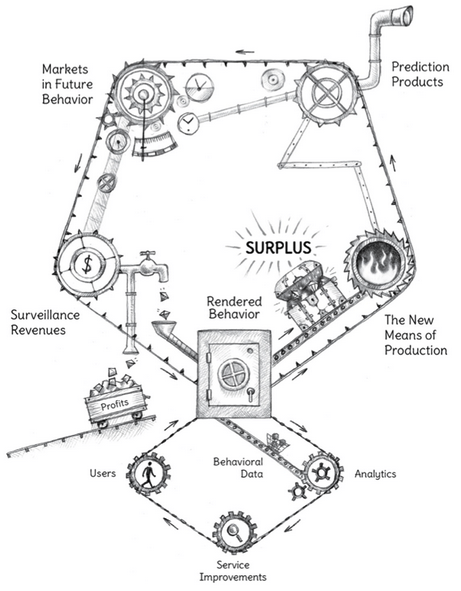
\includegraphics[width=.75\linewidth]{03-theory/zuboff2019.png}
    \captionsetup{justification=centering,margin=1.5cm}
    \caption{The Discovery of Behavioural Surplus \citep[in][]{zuboff2019}}\label{fig: zuboff2019}
\end{figure}

They are not solely focused on fostering individual or even collective curation of democratised art/content. They still employ the capitalist framework at their core. In other words, the extractivist profit motive defines the algorithmic fabric of online `content creation' (production), and resultant social media `engagement' (consumption) through mass data harvesting and advertisement selling. The longer users are engaged on a platform (Facebook, Instagram, Twitter, YouTube, TikTok), the more likely they are to generate profits for the platform via advert click/tap-throughs. Our feeds are interspersed with adverts and sponsored posts that have been carefully curated to maximise the potential click/tap-through rate of their victims. Soshana Zuboff defines this as arising from a `market of human behavioural futures' \citeyearpar{zuboff2019} in her book Surveillance Capitalism. Through this surveillance, large amounts of behavioural, affective, and personal data (termed behavioural surplus by Zuboff) are `skimmed' off the top of our engagement with these platforms, and sold to agencies that match this personal data with products/content you are most likely to engage with. How could it be argued that that the production and consumption of art / content on such platforms is not governed by `private gain' at our expense? 

\begin{figure}[ht]
    \centering
    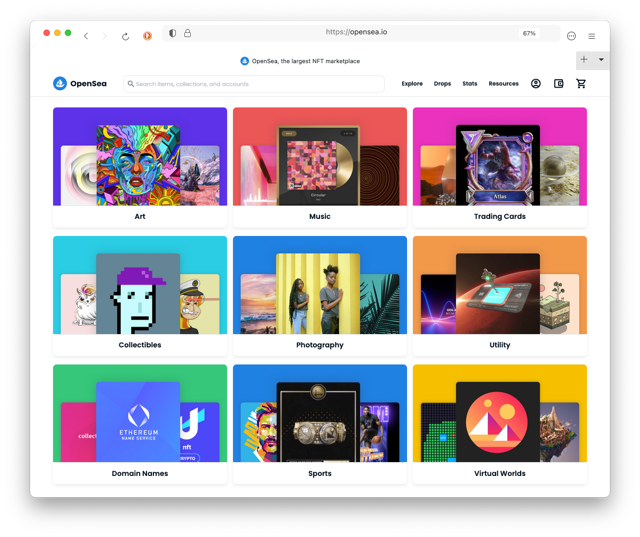
\includegraphics[width=.75\linewidth]{03-theory/opensea2022_1.png}
    \captionsetup{justification=centering,margin=1.5cm}
    \caption{Categories of NFTs being sold on one of the largest NFT marketplaces \citep[from][]{opensea2022a}}\label{fig: opensea2022_1}
\end{figure}

More recently, there are facets of the rise of \gls{nft} art projects that epitomise this continued fetishisation and veneration of digital fine art under the guise of `decentralisation'. Unfortunately enough, these projects often fall foul to the exact `centralisation' they market to oppose, creating small micro-communities of inter-centralised followers that collectively and actively, through social media, ensnare new and uninitiated retail investors via the urgency phenomenon of the `fear of missing out'. The motivation being to increase the value of their own \glspl{nft} - sometimes referred to as `shilling'. In some \gls{nft} projects, the only drive is profit motive, the digital art is merely the vehicle through which this investment is (im)materially realised. Despite the technological basis of some of these projects being quite radical in their proposition of democratic ownership and the privacy and security of digital information through decentralisation, the asset class some of them end up facilitating is tied to a a method of procurement and self-promotion that necessitates the enrichment of the creators and early adopters of that specific \gls{nft} collection. How, in any way, could this method of production and consumption be said to be different from Dewey's outlining of the rise of the `nouveaux riches':
\begin{quote}
    `The nouveaux riches, who are an important by-product of the capitalist system, have felt especially bound to surround themselves with works of fine art which, being rare, are also costly. Generally speaking, the typical collector is the typical capitalist. For evidence of good standing in the realm of higher culture, he amasses paintings, statuary, and artistic bijoux, as his stocks and bonds certify to his standing in the economic world.' \citeyearpar[p. 7]{dewey1934}
\end{quote}
It could be argued therefore, that we have witnessed an increase in the amount of new media formats, but not one that resituates production outside of capitalist logic for the masses; even in so called `decentralised' projects. When Leddy and Puolakka stress that it is this `private control of [the] forces of production for private gain' that leads to this disconnection of art from experience, it follows that the creation of art outside of the confines of this control addresses the imperative for the drawing of art `from all sources' [own emphasis]. From this view, the convergence of digital art to their `conditions of origin and operation in experience' could be seen as one of the primary foci of more recent movements such as Maker, Hacker, and \gls{diy} Labs, as well as the general ethos of participatory design and \glshyperlink[open-source]{opensource} \glshyperlink[hardware]{osh} and \glshyperlink[software]{floss} in art, design, and electronic music practice.

But what does it mean to say that art ought to originate and operate `in' experience, and how might these movements address this? Dewey considers the `live creature' in response to this question. He views the participant of aesthetic experience as meaningfully inseparable from the environment in which they are embedded: 
\begin{quote}
    `The senses are the organs through which the live creature participates directly in the on-goings of the world about [them]. In this participation the varied wonder and splendour of this world are made actual for [them] in the qualities [they experience]. This material cannot be opposed to action, for motor apparatus and `will' itself are the means by which this participation is carried on and directed. It cannot be opposed to `intellect', for mind is the means by which participation is rendered fruitful through sense; by which meanings and values are extracted, retained, and put to further service in the intercourse of the live creature with [their] surroundings.' \citeyearpar[p. 22]{dewey1934}
\end{quote}
From this basis, namely that perception, sensorimotor action, and intellect cannot be meaningfully separated when considering the intercourse of participants with their environment, Dewey highlights the weakness in the traditional dualist / cognitivist model - we are embodied and embedded beings. He posits that experience results from the `interaction of organism and environment',  and that in its fullest, experience can represent a `transformation of interaction into participation and communication'. It would follow, therefore, that in the production of artistic works, consideration of this dynamical relationship that constitutes our subjective experiences is not only valuable, but that artistic works should aim to arise (originate) from common and relatable states of this relationship. Returning art to this origination and operation `in' experience through interactive and participatory digital means can therefore be seen as a crucial mechanism for inducing positive societal change through fostering new channels of `participation and communication'. Shifting the production of artistic work away from the exploitative practices of mass manufacturing inherent in consumer technologies, as well as centring embodied participatory design practices, is a common theme among \gls{diy} and Makerspace communities.

This is not to in any way demean or reduce the social importance of art that does not take these approaches. It is also especially tricky to prove in any certainty the subjective measures of aesthetic experience that could result in positive societal change. However, I do view the imperative to shift production and consumption of art outside the capitalist architecture of current proprietary software tools and consumer technologies, and bringing the aesthetic closer to every day experience as a fruitful endeavour for the artist. I argue that doing so would emphasise the dynamical relationship participants find themselves in with their and, crucially, others' sociocultural, economic, and ecological contexts.

Where does knowledge lie for us as researchers in the production and consumption of such artistic works? On what basis can we test and evaluate these claims? One view that is popular in the field of music technology is that of considering the nature of the interactive and digital systems that we develop; a consideration of the epistemic tool. 
\begin{quote}
    `The digital instrument is an artefact primarily based on rational foundations, and, as a tool yielding hermeneutic relations, it is characterised by its origins in a specific culture. This portrayal highlights the strengthened responsibilities on the designers of digital tools, in terms of aesthetics and cultural influence, as they are more symbolic and of compositional pertinence than our physical tools.' \citep[p. 335]{magnusson2009a} 
\end{quote}

Developed by Magnusson, this line of thinking proposes that the digital instruments we design and employ as artists have inscribed in their physicality, affordance and sonic output, knowledge of cultural, historical, and designerly significance. In this way, they can be considered complex systems of research importance through the examination of their symbolic design, construction, performance, and appreciation by audiences. Magnusson embeds this proposition within Don Ihde's philosophy of `instrumental realism' and Wittgenstinian philosophy, and draws from an understanding of the extended mind hypothesis. This theory, which will be expanded on in the next section, proposes that 
\begin{quote}
    `[Under certain conditions], the human organism is linked with an external entity in a two-way interaction, creating a coupled system that can be seen as a cognitive system in its own right.' \citep[p. 7]{clark1998}
\end{quote}


Similar to Dewey's conception of how the live creature is inseparable from the environmental conditions that it is embedded in, the extended mind hypothesis and similar theories of embodied cognition prove to be invaluable in the field of tangible user interfaces, and \gls{dmi} design, due to the way they can explicate as well as draw out the dynamic relationships between artist, collaborator, material, interface, and audience in the deployment of expressive artistic media. In the following sections, I shall dive deeper into these theories of embodiment, and what they have to offer a practice that makes use of \gls{ar} technologies within the field of computational art and musical performance.

\begin{figure}[h]
    \centering
    \includegraphics[width=1\linewidth]{03-theory/úlfarsson2014.png}
    \captionsetup{justification=centering,margin=1.5cm}
    \caption{An early Halldorophone (cello-like feedback instrument) \citep[from][]{ulfarsson2014}}\label{fig: ulfarsson2014}
\end{figure}

% --------------------------------------------------------------------------- %
\section{The 4E Approach to Experience}\label{sec: theory-4e}
One way of expanding on this conception of aesthetic experience is to adopt the an increasingly popular approach to conceptualising experience called enactivism. Key to my following theoretical underpinning of materiality, embodiment, and space will involve how this approaches the themes of perception, agency and cognition arising through the complex inter-threaded coupling between a participant and their environment. Often referred to as `the 4 E's', \gls{4ec}, states that cognition is an \textit{embodied}, \textit{embedded}, \textit{enactive}, and \textit{extended} process \citep{gallagher2017}. It's worth mentioning that \gls{4ec} is an amalgamation of theories across the disciplines of philosophy and the social and cognitive sciences, and as such there are different flavours of it. Many of these have said to have roots in the Dewey's (among others') pragmatism outlined in the previous section, as well as Merleau-Ponty's embodiment theories \citep{zavota2016}. What these constituent theories all bear in common is the rejection of the standard cognitivist model of experience that states that cognitive processes happen solely `in the mind' and 'in the brain'. Another principle is that they generally draw from complex systems theory: `understanding the complex interplay of brain, body and world requires the tools and methods of nonlinear dynamical systems theory' \citep{clark1999}. Before delving into the specification and implications of a \gls{4ec} approach, I would first like to touch on this concept of complexity, as it will surface throughout the thesis. Within certain systems, which are deemed to be `complex', this field proposes that there are a multitude of phenomena that can explicate the interactions between components of such a continually unfolding system, including \citep{dedomenico2019}:
\begin{itemize}
    \item Interactions - a complex system is formed of many components, many of which will be connected in a network of mutual and on-going interaction
    \item Emergence - from this network of interactions, there exists the possibility for complex and novel structures to form that are inexplicable from the features of their simpler components 
    \item Dynamics - the state of a complex system can change over time, often in an unpredictable non-linear fashion
    \item Self-organisation - the components of a complex system may exhibit collective behaviours, and perceived large scale structure
    \item Adaptation - complex systems don't necessarily shift between steady states, they actively and reactively respond to environmental stimuli
    \item Feedback - structures of a complex system exhibit a phenomena where the outputs of a system are routed back in, via closed chains of cause and effect 
\end{itemize}

\begin{figure}[ht]
    \centering
    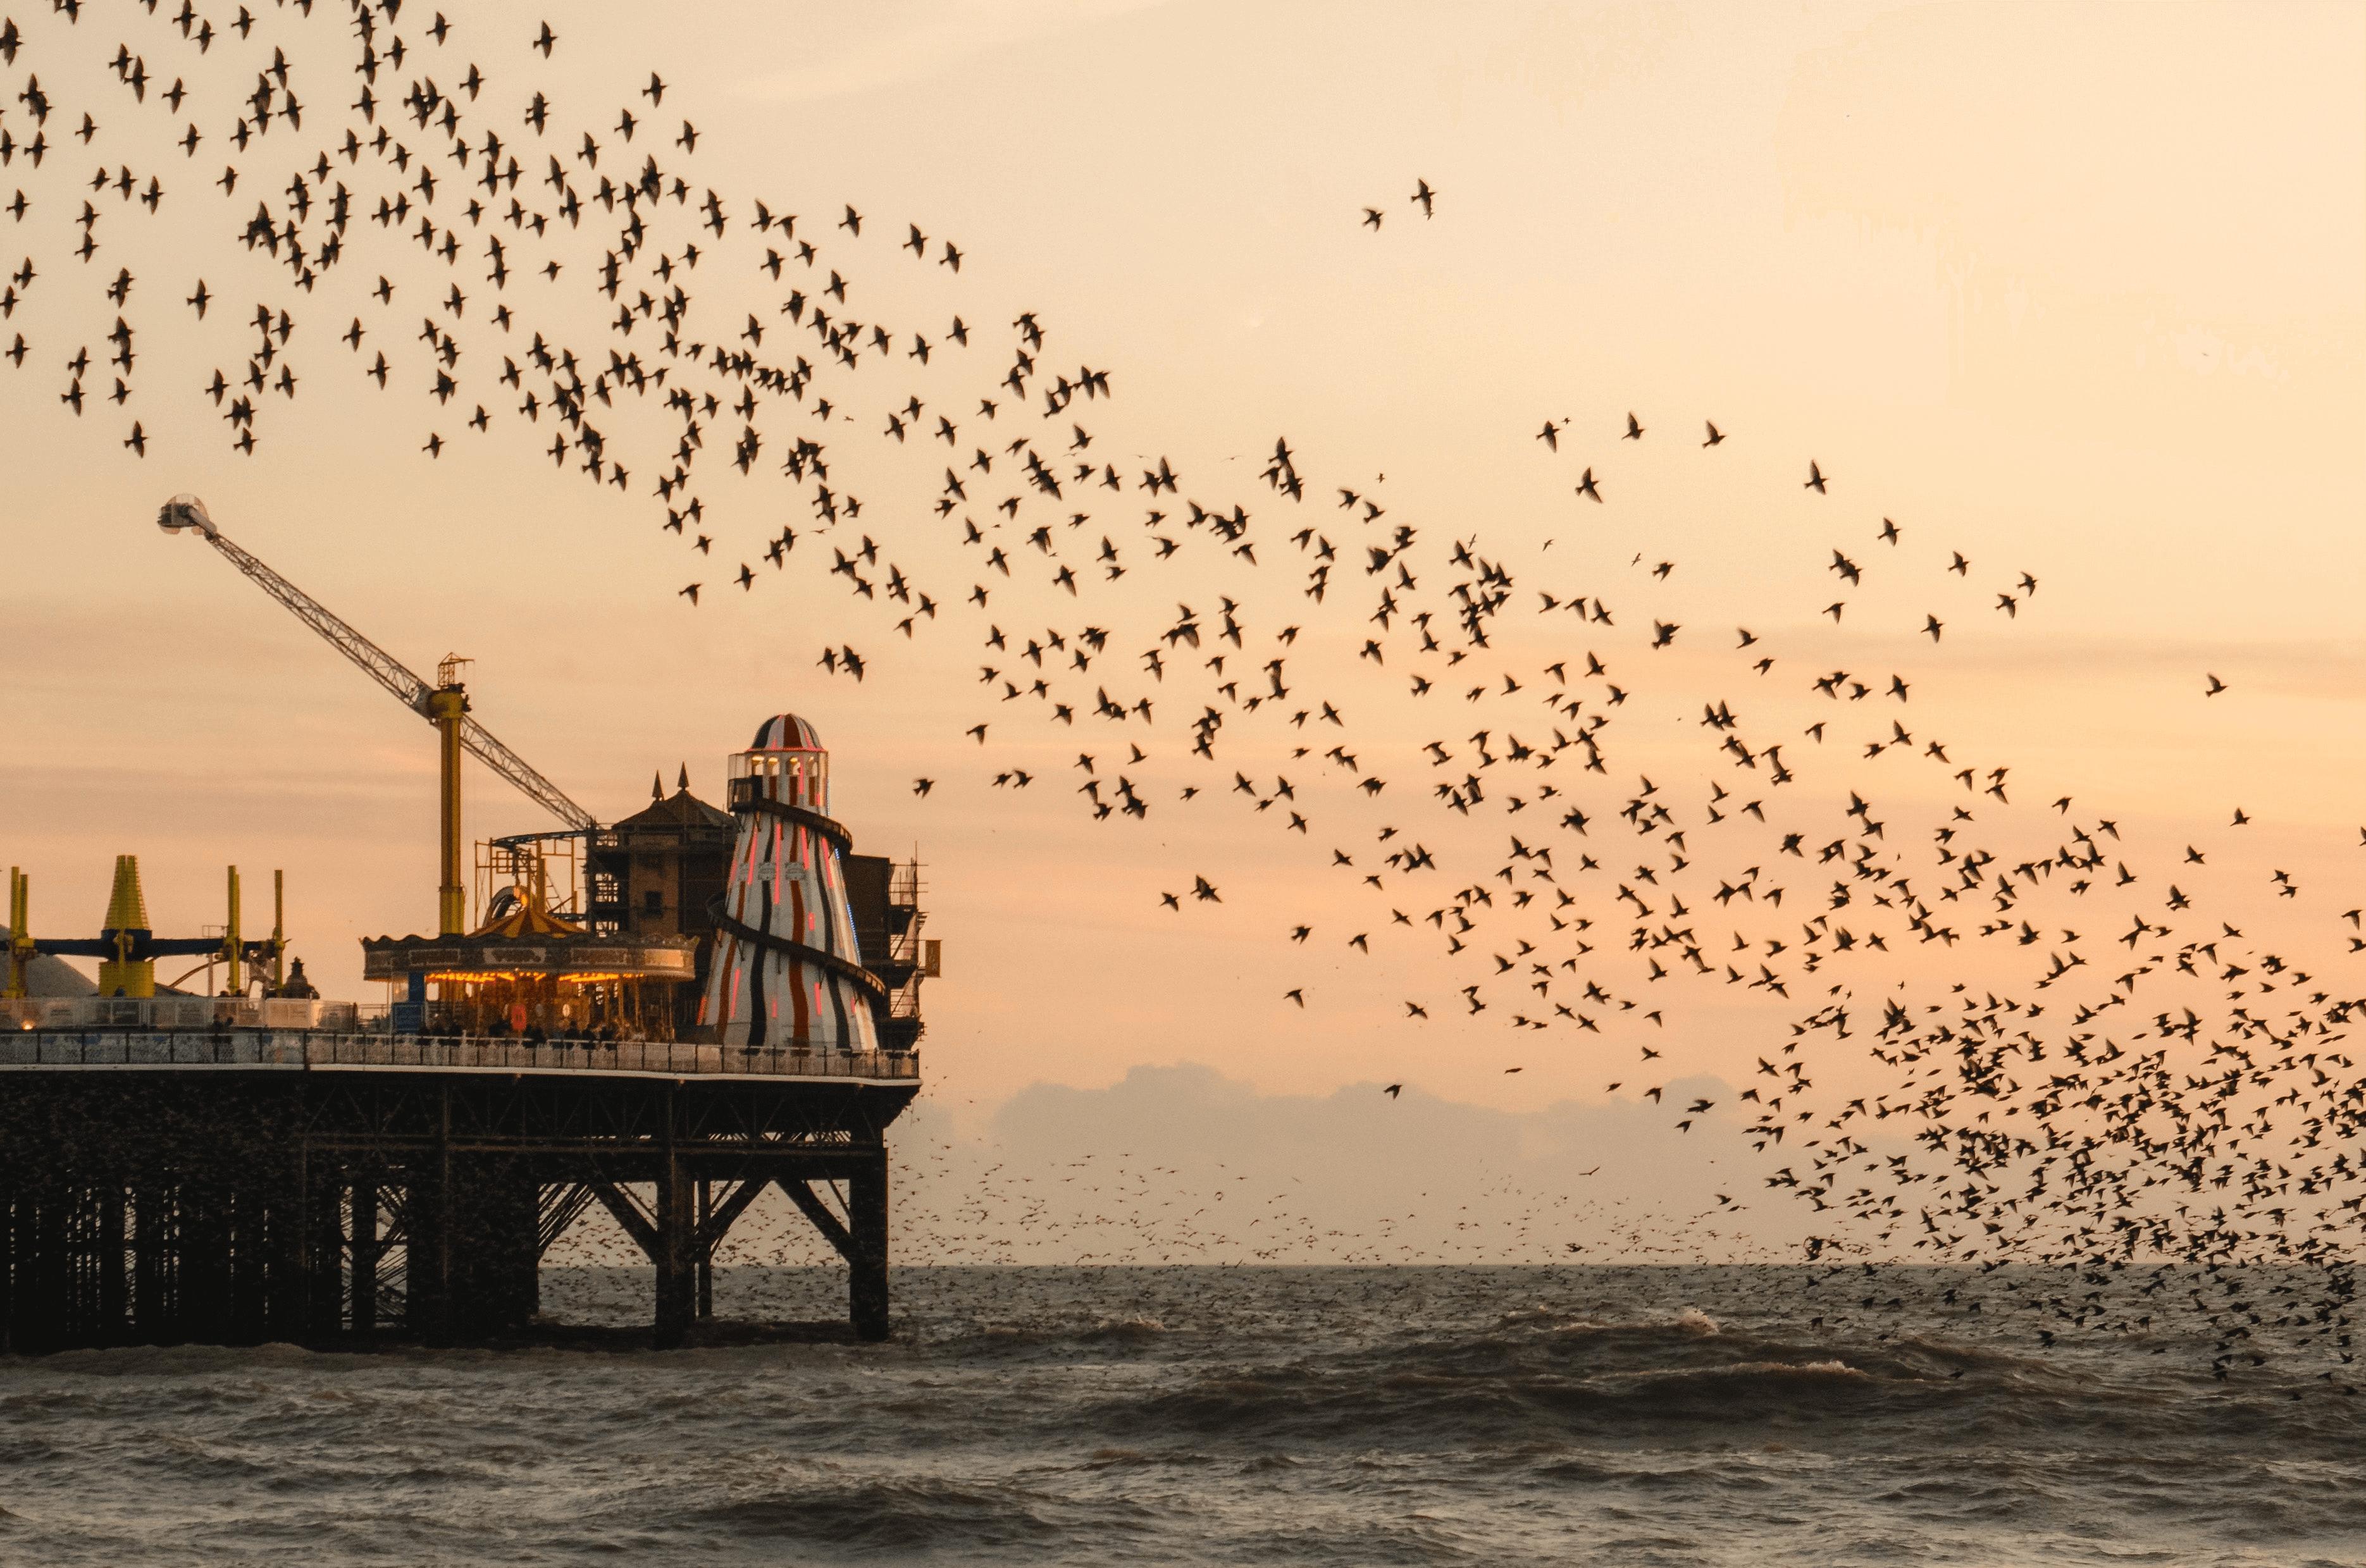
\includegraphics[width=.65\linewidth]{03-theory/kentish2020.png}
    \captionsetup{justification=centering,margin=1.5cm}
    \caption{Starling murmuration displaying complex and emergent flocking behaviours \citep[taken by][in Brighton, UK]{kentish2020}}\label{fig: kentish2020}
\end{figure}

%% !!! check here, ben white
Thus, \gls{4ec} normally begins with an acknowledgement of the complex embodied nature of human cognition. Varela, Thompson, and Rosch propose that cognition is embodied in a way not too dissimilar to the assertion Dewey holds in regards to the `senses' of the `live creature'.
\begin{quote}
    `By using the term embodied we mean to highlight two points: first, that cognition depends upon the kinds of experience that come from having a body with various sensorimotor capacities, and second, that these individual sensorimotor capacities are themselves embedded in a more encompassing biological, psychological, and cultural context.' \citeyearpar[pp. 172-173]{varela1993}
\end{quote}
Alva Nöe's concept of sensorimotor contingencies has since built on the first point of this approach to embodiment, in a way that proposes an `enactive approach to perception' accepts that perception is something we do, not something that happens to us \citep{noe2004}. This has since been termed the `sensorimotor approach' to enactivism, and Gallagher notes that it falls short of an `enactivist approach' due to its omission of affective aspects of embodiment such as `mood-related and emotional factors, […] bodily states such as hunger, fatigue, and pain, as well as a complex motivational dimension that animates body-world interaction' \citep[p. 150]{gallagher2017} The proposal is that that an `enactivist' approach, i.e. one that aligns with Varela, Thompson, and Rosch's claim that sensorimotor capacity is `embedded in biological, psychological, and cultural contexts' more holistic perspective, the proponents of embodiment theories of \gls{4ec} propose a radical shift from the standard cognitivist model; sensory perception and bodily existence is not only causally related to the emergence of cognitive processes, it literally constitutes them. 

A natural continuation extends this line of reasoning to the material environment in which the participant is a part of — accepting that it is in turn shaped by the web of sociocultural norms and values that Dewey alludes to, and is the site of sensorimotor action. Mark Rowlands proposes this underlying thesis as `the embedded mind':
\begin{quote}
    `In accomplishing cognitive tasks, an organism can utilize structures in its environment in such a way that the amount of internal processing it must perform is reduced. Some of the complexity of the task is, thereby, off-loaded onto the environment, given that the organism has the ability to appropriately exploit that environment.' \citeyearpar[p. 68]{rowlands2010}  
\end{quote}
It necessarily follows that if a cognitive system that has the potential for environmentally embedded sensorimotor action, i.e. it is embodied and embedded, it also enacts its cognition. The first formal account of what could be called an enactive approach to cognition begins also in `The Embodied Mind', by Varela, Thompson and Rosch. From a foundation of accepting that sensory and motor processes, namely perception and action, are `inseparable in lived cognition', enaction is contingent on two assumptions: perception consists in perceptually guided action, and cognitive structures emerge from the recurrent sensorimotor patterns that enable action to be perceptually guided \citeyearpar[p. 173]{varela1993}. The authors argue that an enactive approach to cognition therefore proposes that perception must be studied from the point of view of the participant's sensorimotor structure, rather than any `pre-given, perceiver-dependent world', i.e. the world is not perceived through an internal representational model of what is `outside', rather, the world emerges from a participants ability to `guide [their] actions in [their] local situation', to enact.

The last assertion of a \gls{4ec} account claims that cognition has the potential to be extended into objects in a participants environment. The extended mind hypothesis, as developed by Andy Clark and David Chalmers and described in the previous section, is the core thesis of this proposal. The authors propose that, cognitive processes, beliefs for example, can be `constituted partly by features in the environment, when those features play the right sort of role in driving cognitive processes' \citeyearpar[p. 12]{clark1998}. They compare the experience of cognition in two different hypothetical people, Inga and Otto. Both are tasked with recalling the address of the \gls{moma} and travelling to it. Inga has a neurotypically functioning memory, and so accesses the memory of the address (which assumedly lay dormant previous to this action) recalls it, and travels to the address. Otto has Alzheimers, and like many others with Alzheimers relies on the use of a notebook or memory aid to recall experiences and other important information, he finds the address in the notebook, and travels to the museum. In both cases, Clark and Chalmers propose that the cognitive functionality of what constitutes 'belief' are analogous:
\begin{quote}
    `To say that the beliefs disappear when the notebook is filed away seems to miss the big picture in just the same way as saying that Inga's beliefs disappear as soon as she is [no] longer conscious of them. In both cases the information is reliably there when needed, available to consciousness and available to guide action, just the way that we expect a belief to be' \citeyearpar[13]{clark1998}.
\end{quote}

\begin{figure}[ht]
    \centering
    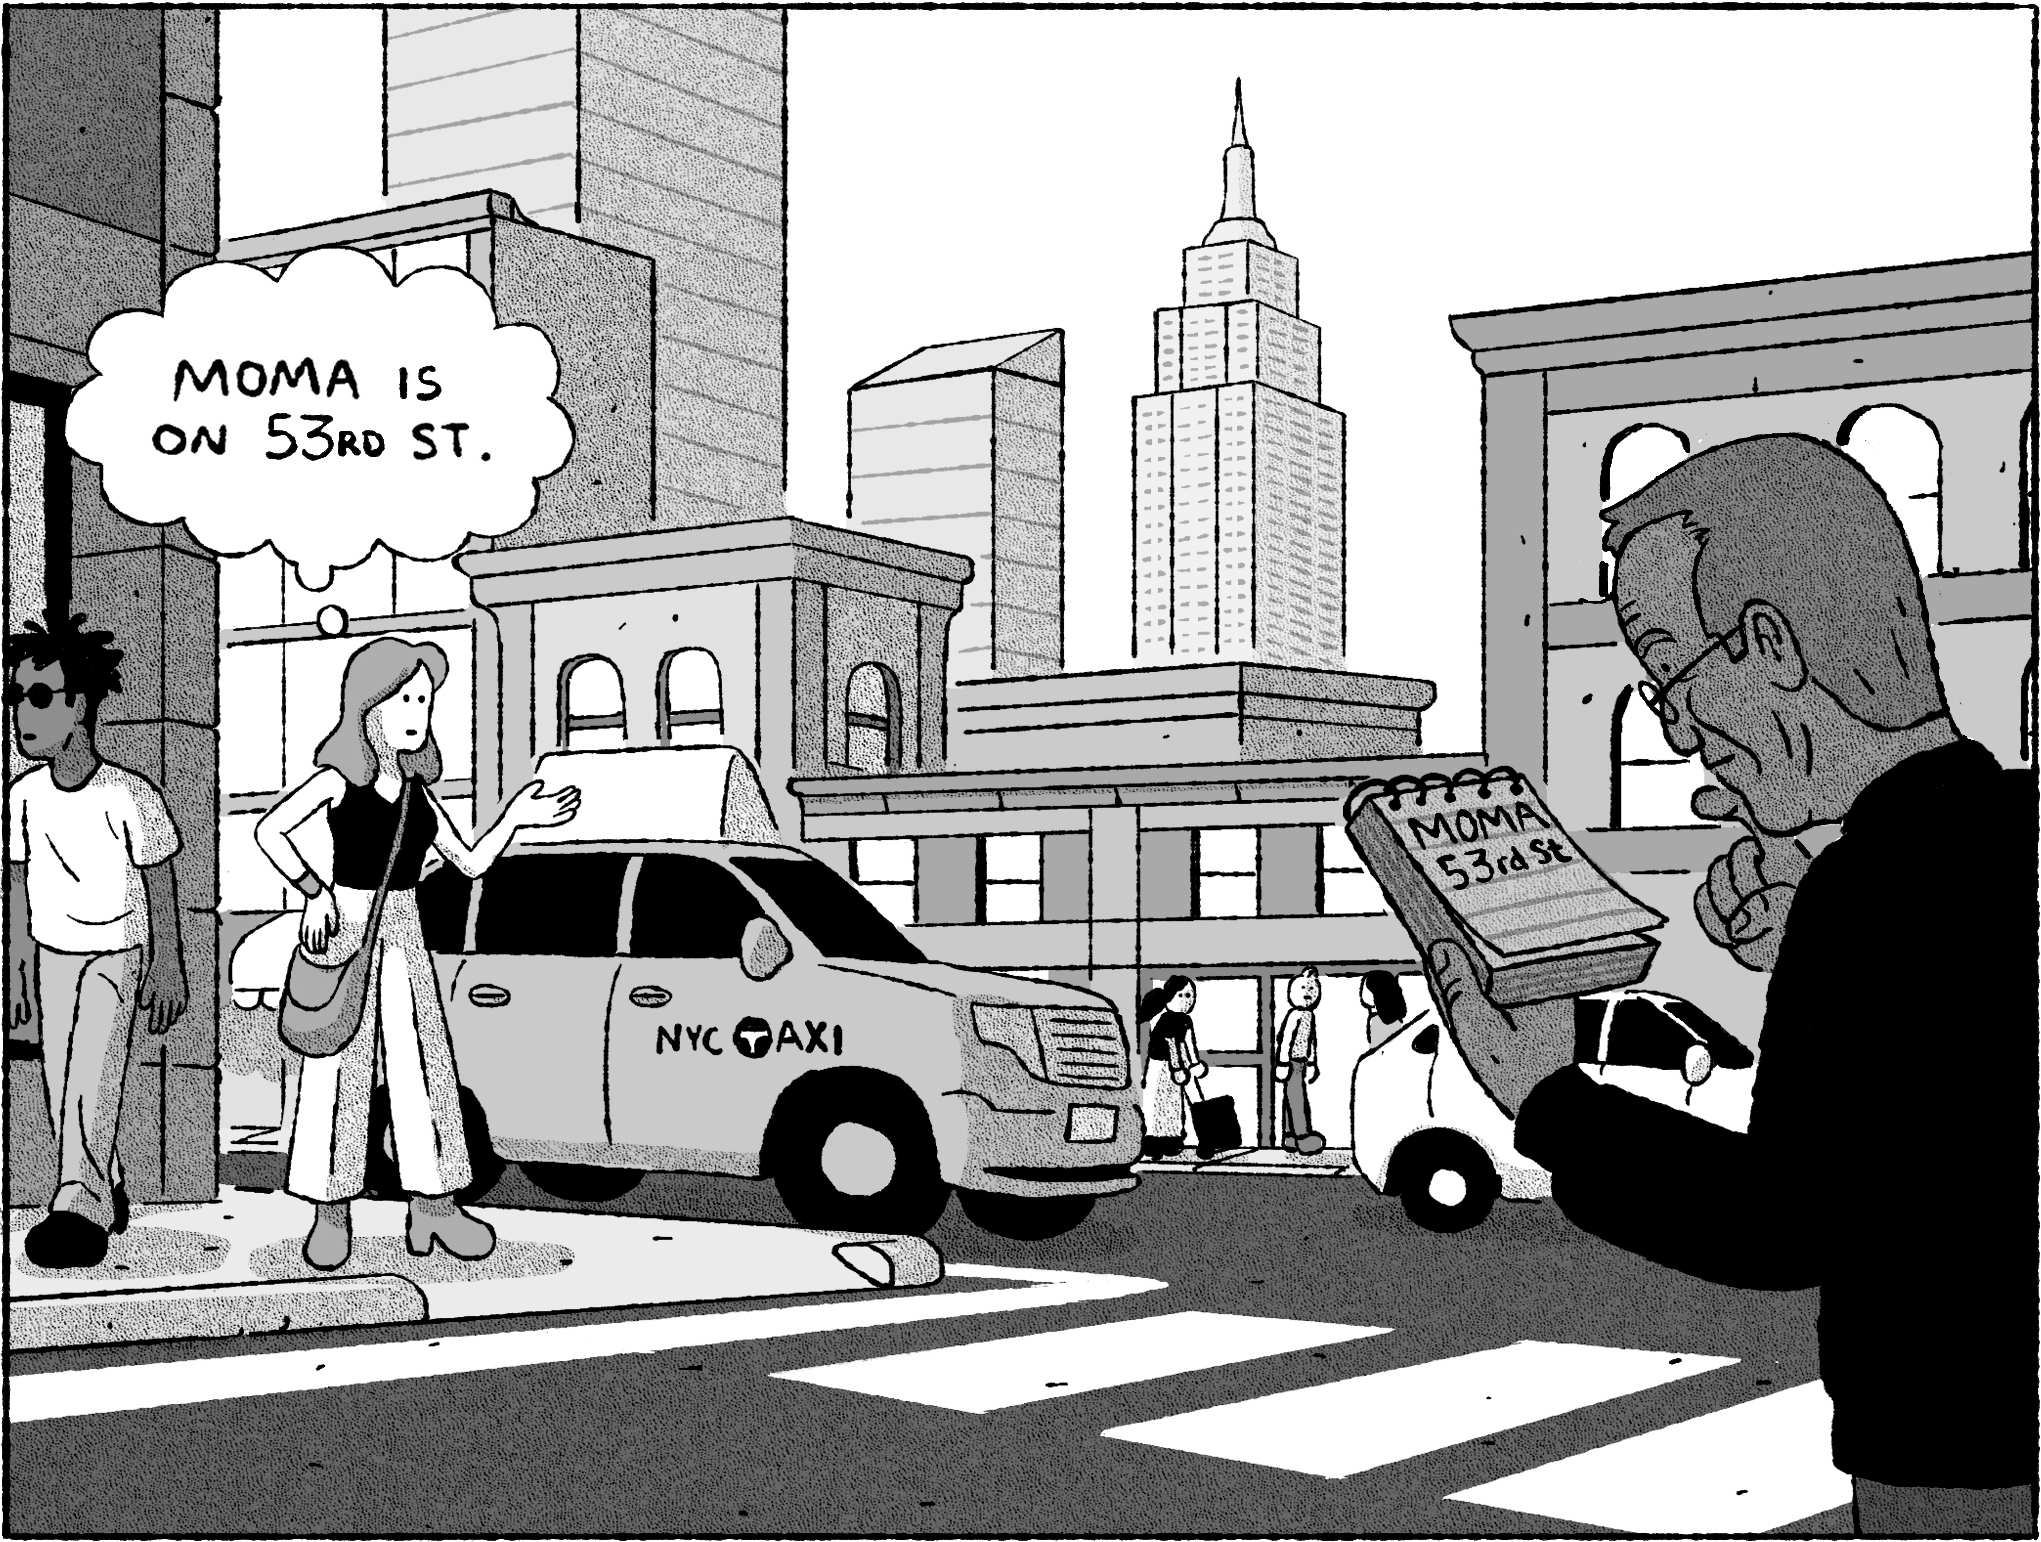
\includegraphics[width=.75\linewidth]{03-theory/chalmers2022_1.png}
    \captionsetup{justification=centering,margin=1.5cm}
    \caption{Inga and Otto on their way to the MoMA \citep[by Tim Peacock in][]{chalmers2022}}\label{fig: chalmers2022_1}
\end{figure}

It therefore follows, that cognition is extended, beyond the boundary of the mind-body and into the environment, and even into specific artefacts - a key theory that enables the proposition of Magnusson's epistemic tool within the field of music technology, as mentioned previously. Taking these four points of departure, namely that cognition is embodied, embedded, enacted, and extended, Gallagher presents the following assumptions as the core conditions of an enactivist approach to cognition \citep[p. 6]{gallagher2017}:
\begin{enumerate}
    \item Cognition is not simply a brain event. It emerges from processes distributed across brain – body – environment. The mind is embodied; from a first-person perspective embodiment is equivalent to the phenomenological concept of the lived body. From a third-person perspective the organism–environment is taken as the explanatory unit.
    \item The world (meaning, intentionality) is not pre-given or predefined, but is structured by cognition and action
    \item Cognitive processes acquire meaning in part by their role in the context of action, rather than through a representational mapping or replicated internal model of the world
    \item Enactivist approaches have strong links to dynamical systems theory, emphasising the relevance of dynamical coupling and coordination across brain – body – environment
    \item In contrast to classic cognitive science, which is often characterised by methodological individualism with a focus on internal mechanisms, enactivist approaches emphasize the extended, intersubjective, and socially situated nature of cognitive systems. Enactivism aims to ground higher and more complex cognitive functions not only in sensorimotor coordination, but also in affective and autonomic aspects of the full body.
    \item Higher-order cognitive functions, such as reflective thinking or deliberation, are exercises of skilful know-how and are usually coupled with situated and embodied actions
\end{enumerate}
Poignantly, this way of framing our human experience is salient for the digital humanities at this point in time. More of our everyday social, artistic, political, cultural, environmental, and economic interactions are mediated by technologies and platforms. These are privately owned by mega-corporations, that as previously mentioned, have shown dubious a relationship with ethics concerning misinformation and user privacy, as well as extractivist methods of guaranteeing shareholder profit. Does Facebook's `metaverse' sound like the kind of \gls{ar} environment that sounds like a safe and democratic ground for art that seeks the `transformation of interaction into participation and communication' \citep[]{dewey1934}? This decision is up to the reader, but I would argue not as it will become clear in the following sections.

Out of this model of explicating experience, I propose three lenses through which to examine \gls{ar} applications in the sonic arts - materiality, embodiment, and spatiality. In some ways, a linear, written account of these processes, separated neatly by subheadings is somewhat incompatible with the logic of \gls{4ec} and its process-inseparability, nevertheless, in the following sections of this chapter I will attempt to go into detail how we can use this model of experience, to consider the themes of materiality, embodiment, and space within \gls{ar} musical instrument research practice, as well as the broader study of digital humanities. Loosely, these three sections will cover the artistic, audience, and societal considerations and potentialities respectively, when engaging with \gls{ar} systems.



% --------------------------------------------------------------------------- %
\section{Complex Material in Interactive Music Systems}\label{sec: theory-materiality}
Thus far, we have outlined the contextual origins of \gls{ar} technology, as well as their contemporary physical forms, modes of sensory display, and methods of real and virtual processing. Additionally, I have outlined the theories of aesthetic and perceptual experience through which these technologies could be interrogated to further understand \gls{ar}'s role as a medium for artistic expression. In this section I will propose a lens through which to consider the artist's composition of `material' in \gls{ar} experiences as a method of fostering a modulated dialogue between elements of a participants sensorimotor engagement with their perceived real and virtual environment.

Existing frameworks for considering the design of relationships between real and virtual processes do exist within in the field of \gls{ar}; in the early 90's, the theoretical work of Milgram and Kishino, their reality-virtuality continuum \citeyearpar[p. 10]{milgram1994}, proved to be a fruitful way of sorting the types of \gls{ar} and \gls{vr} technologies that were arising from different fields at the time. However, for my purposes of detailing the material nature of an artists' composition in \gls{ar}, a more nuanced and detailed framework is needed, one that goes beyond specifying the what (a spectrum of reality to virtuality); towards a investigating of the how, (a processual space of augmentation, diminution, alteration, hybridisation, and extension through which real and virtual environments are enmeshed), and the why (the conveyance of meaning and intentionality of the artistic work). 

Hanna Schraffenberger, as highlighted in \autoref{sec: ar-process}, offers a set of relations that describe the dynamics between `the virtual and the real' (see \autoref{table:schraffenbergertaxonomy}, \pageref{table:schraffenbergertaxonomy}). She argues that from the fundamental relationships of presence, information, physicality, and behaviour, there emerge new `subforms' of \gls{ar}, namely extended, diminished, altered and hybrid reality, as well as extended perception. Yet, even with this level of description, the processes themselves are still abstract - these are descriptors for the types of processes, but what are the processes themselves? I believe that the answer lies again, in an approach aligned with complex systems theory; through a consideration of phenomena such as interaction, emergence, dynamics, self-organisation, adaptation, and feedback.

\begin{wrapfigure}{r}{0.45\textwidth}
    \vspace{-\intextsep}
    \hfill
    \begin{minipage}{0.95\linewidth}
        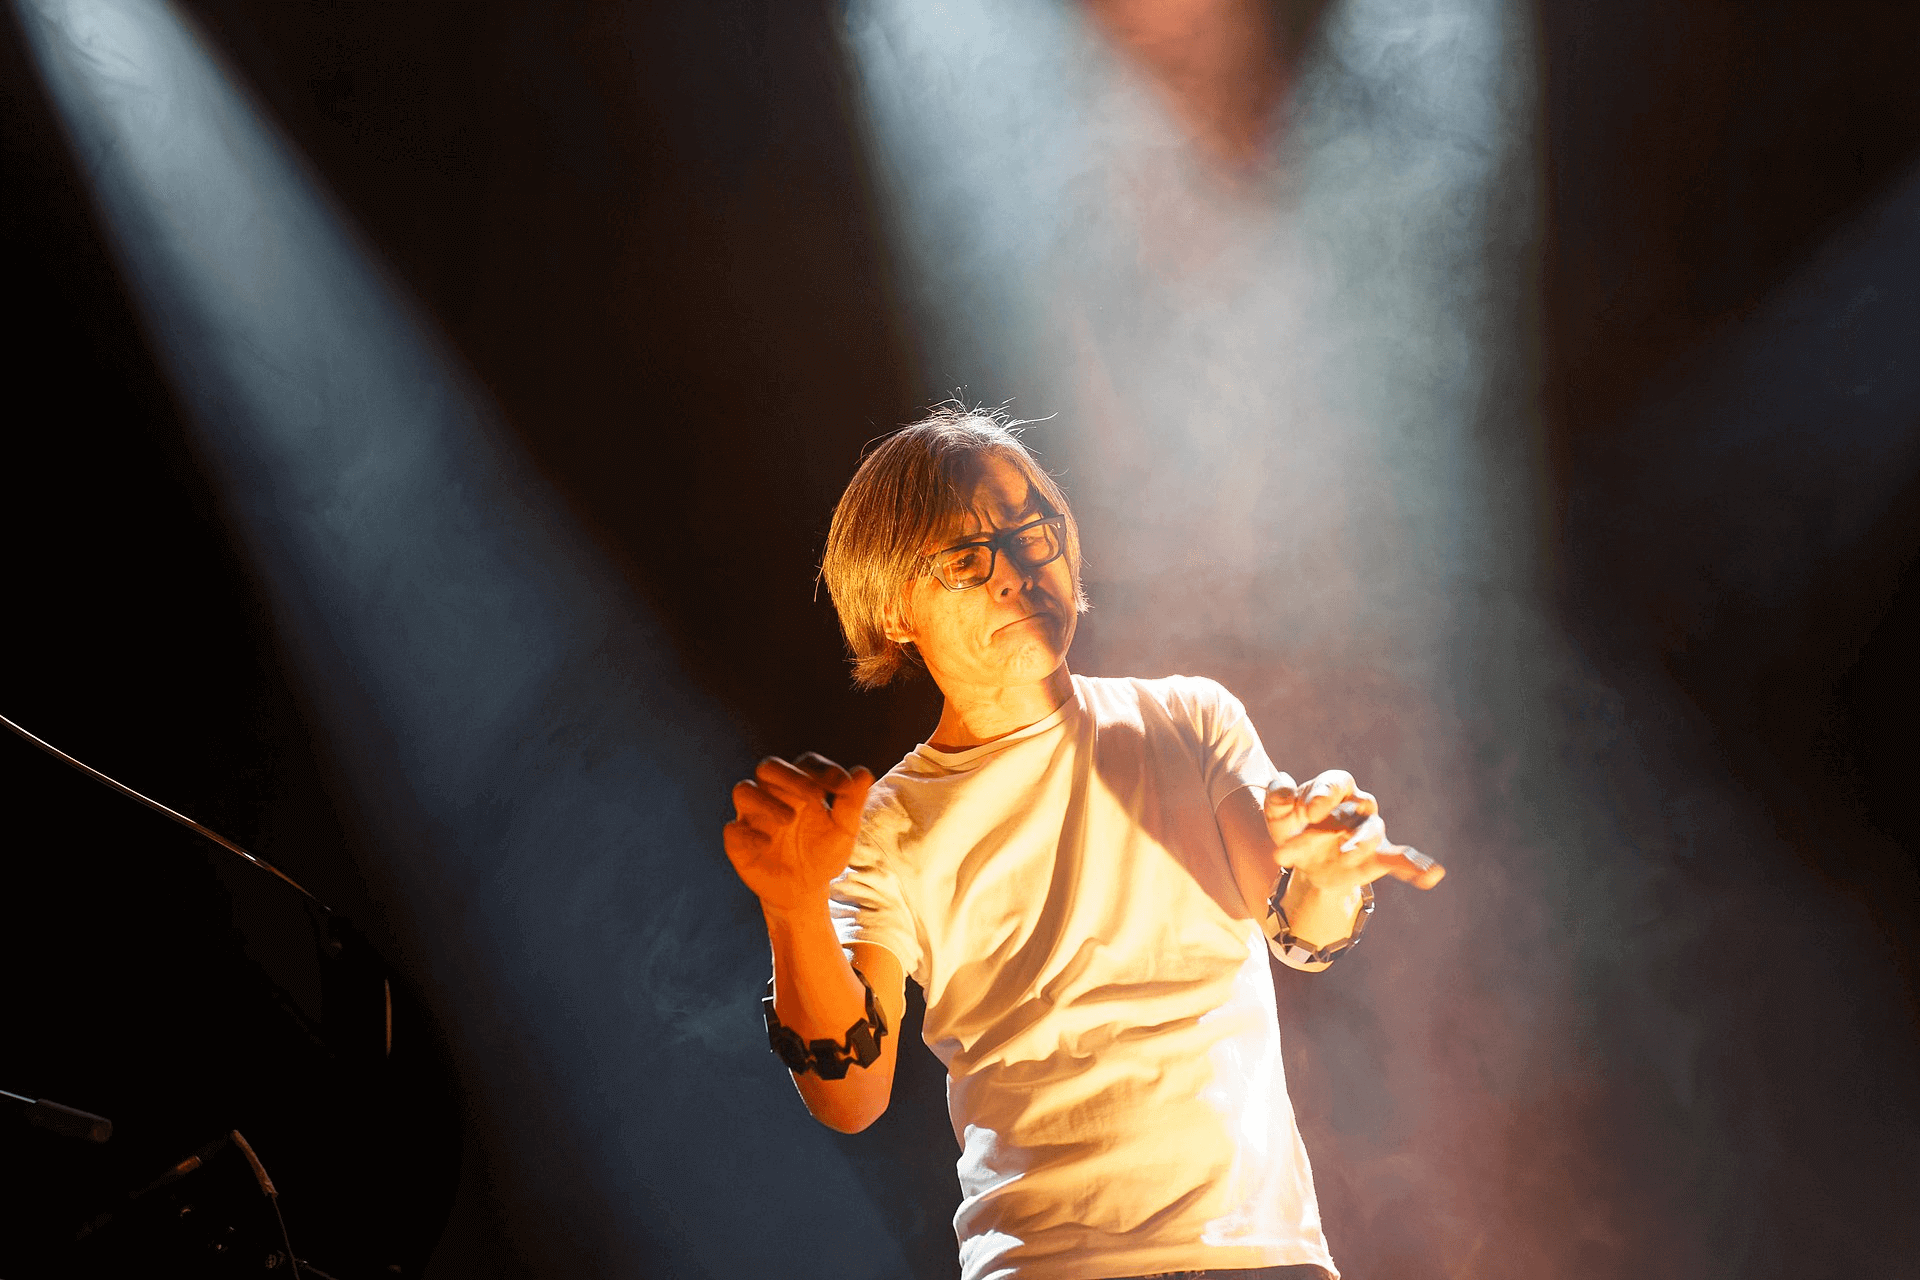
\includegraphics[width=\linewidth]{03-theory/delaney2017.png}
        \captionsetup{justification=justified}
        \caption{Atau Tanaka performing \textit{Myogram}, an 8 channel sonification of muscular corporeal states \citep[taken by][]{delaney2017}}\label{fig: delaney2017}
    \end{minipage}
\end{wrapfigure}

Within the field of music interfaces, considerable research and practice has been conducted in the area of complex systems. Surmised neatly by musical interface researcher Joel Ryan, hidden, or black-boxed complex processes within digital interfaces can be developed and explored through ascribing `physical handles' to these `phantom models', e.g. providing embodied interaction to algorithmic musical processes to better understand, design, and evaluate them.
\begin{quote}
    `The physicality of the performance interface helps give definition to the modelling process itself. The physical relation to a model stimulates the imagination and enables the elaboration of the model using spatial and physical metaphors. The image with which the artist works to realise his or her idea is no longer a phantom, it can be touched, navigated and negotiated with.' \citeyearpar[p.5]{ryan1991}
\end{quote}
Perhaps the design of \gls{ar} musical instruments is concerned with not only providing physical handles to phantom models, but phantom handles to physical models too.

In the same vein, Agostino Di Scipio outlined his perspective on the paradigm of interaction in the context of audio signal processing and musical interface use. 
\begin{quote}
    `Interactive music systems are dedicated computational tools capable of reacting in real time, upon changes in their `external conditions', [typically including] initial input data and run-time control data […] set, changed and adjusted by some agent – a performer, or group of performers […] Control devices, with their mechanical and/or visual interfaces, are operated to determine these data.\\ 

    The main purpose of control data is to determine a system's changes of internal state. This is done indirectly, by updating the parameters in either digital signal processing techniques or program routines operating at a more abstract, symbolic level. Changes of internal state are heard as changes in the musical output. By operating the available control devices, the agent in effect `plays' the system as if it were a new kind of music instrument' \citeyearpar[p. 1]{discipio2003}
\end{quote}
For Di Scipio, the act of integrating the agent / performer into the definition of the music system implies that 'interaction' exists in the `underlying ontology' or `interdependent coupling' of participant and instrument; at the site of their `interface'. This coupling creates linear feedback loops in performance, between the resultant sound, and decisions made by the performer. Indeed, this lower-level dependency (human-machine) itself exists within the wider `meta-system' including `[human], machine and environment'. Within this meta-system, later referred to as an `ecosystem', Di Scipio outlines that:
\begin{quote}
    `A principal aim would be to create a dynamical system exhibiting an adaptive behaviour to the surrounding external conditions, and capable to interfere with the external conditions themselves. Not only would it be able to detect changes in the external world and `hear' what happens out there, […] it would also be able to become a self-observing system, that is, to determine its own internal states based on the available information on the external conditions – including the traces of its own existence left in the surroundings. […] This [move towards composing musical interactions] should be described as a shift from creating wanted sounds via interactive means, towards creating wanted interactions having audible traces. In the latter case, one designs, implements and maintains a network of connected components whose emergent behaviour in sound one calls music.' \citeyearpar[p. 6]{discipio2003}
\end{quote}

The depth of research based on this type of complex interactive music system (IMS) has deepened considerably in the last 20 years, as artificial intelligence and machine learning algorithms, low-latency microcontrollers, and real-time compositional software have been implemented into what Magnusson terms `intelligent instruments' \citeyearpar[p. 8]{magnusson2009}. Thus, `performative ecosystems' \citep[]{waters2007} such as these exhibit behaviours of complex systems as mentioned above, including interaction, emergence, dynamics, self-organisation, adaptation, and feedback. I propose therefore that an enactivist approach to experience \gls{4ec}, one that posits the emergence of cognitive processes across the distributed system of mind-body-environment as being wholly appropriate in the design, creation, performance, an evaluation of interactive music ecosystems. 


\begin{wrapfigure}{l}{0.45\textwidth}
    \begin{minipage}{0.95\linewidth}
        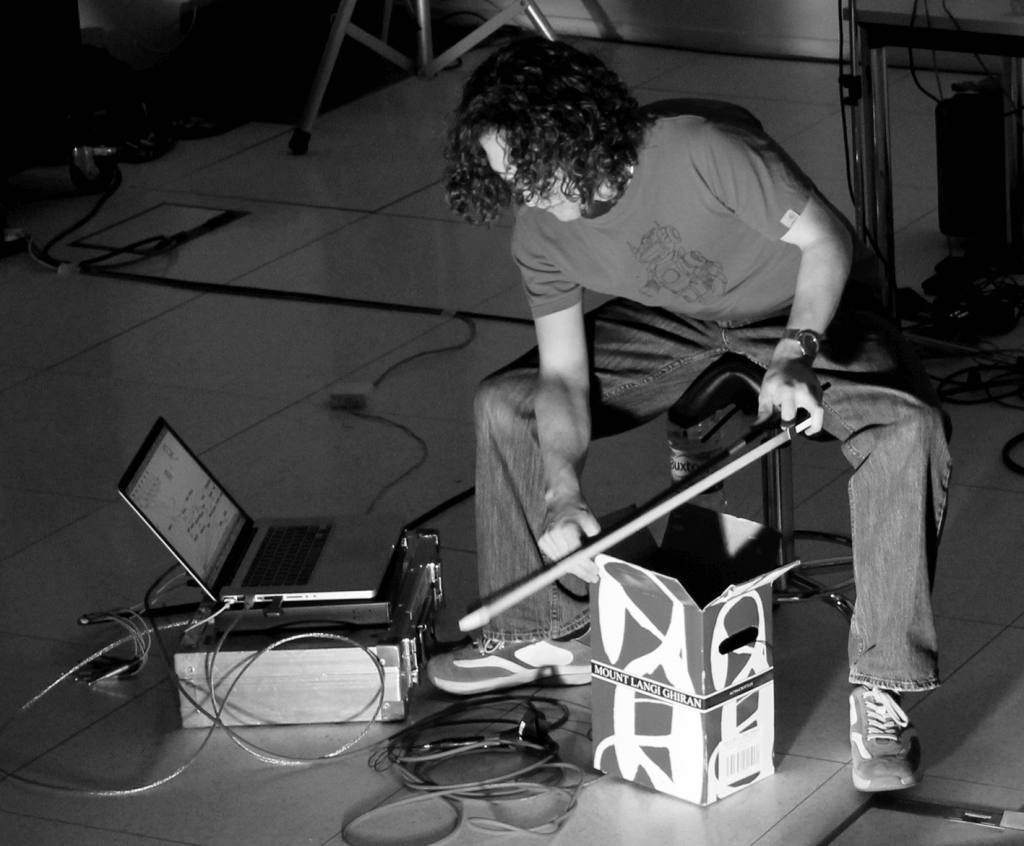
\includegraphics[width=\linewidth]{03-theory/green2010.png}
        \captionsetup{justification=justified}
        \caption{Bowed Cardboard Box in performance \textit{Cardboard Cutout} \citep[from][]{green2010}}
    \end{minipage}
    \hfill
\end{wrapfigure}
Some of the first proponents of this approach include Essl and O'Modhrain, who propose an enactive approach they term `weak sensorimotor integration' to the design philosophy of tangible interfaces for musical expression. `What concerns us here[…], is the consideration of enactive knowledge in the context of musical instrument design and how perceptually guided action defines the `feel' and playability of a musical instrument.' \citeyearpar[p. 3]{essl2006}. Core to their research is the question: `In what way does a specific integration of sensory perception and motor action correspond to a controllable, even enjoyable musical performance experience?' Building on the class of expected sounds that correlate to our action with physical objects in the world, Essl and O'Modhrain evaluate the design of a set of prototype tangible interfaces that introduce a flexibility in this expectation-realisation coupling between action and sound by altering the digital sonic output of the system based on measured user interaction. They propose that the resultant interaction with these instruments provided grounds to include a loose sensorimotor integration into the design of musical interfaces. The present thesis is interested in the implication of this hypothesis in the creation of not only physical interactions with IMS, but also virtual, and ultimately, hybrid interactions. My own \gls{4ec} approach to the compositional material of \gls{ar} musical experiences draws from Essl and O'Modhrain's own motivation for their proposal of an enactive approach. How are dynamics of \gls{ar} musical systems learnt over time? How is the ability to predict musical outcomes affected by the integration real-time motion sensing and parameter mapping? How does the configuration of hybrid sensory content define the way action becomes perceptually guided?

Newton Armstrong also provides considerable insight on the enactive design of \glspl{dmi}. He proposes an `enactive model of interaction' that is concerned with `circular chains of embodied interdependency between performer and instrument, instrumental `resistance' to human action and intentionality, and an integrative approach to the roles of sensing, acting and cognitive process in the incremental acquisition of performative skill.' For Armstrong, this approach draws from a principled distinction between `functional' and `realizational' interfaces. Whereas a functional interface `serves a predetermined function; it is structured around a finite set of interactions which are known in advance of the task's execution', a realizational interface `brings with it the possibility of continuously realizing new encounters and uses, and, in the process, of re-determining the relationship between technical objects and their human subjects' \citep[p. v]{armstrong2006}. This distinction, and a pursuit of the latter over the former, means to prioritise the contexts of `meaning and signification in which human and medium are embedded, and is conducive to dynamic and indeterminate forms of interaction' (p.42). These dynamic forms of interaction are realised through performer intention, and instrumental `resistance' in response the performer's engagement with it. Over time, this resistance establishes adaptation in participant interaction, constituting what Armstrong terms a `dynamical responsiveness' between the performer and their instrument (pp.46-47). 

\begin{wrapfigure}{r}{0.45\textwidth}
    \vspace{-\intextsep}
    \hfill
    \begin{minipage}{0.95\linewidth}
        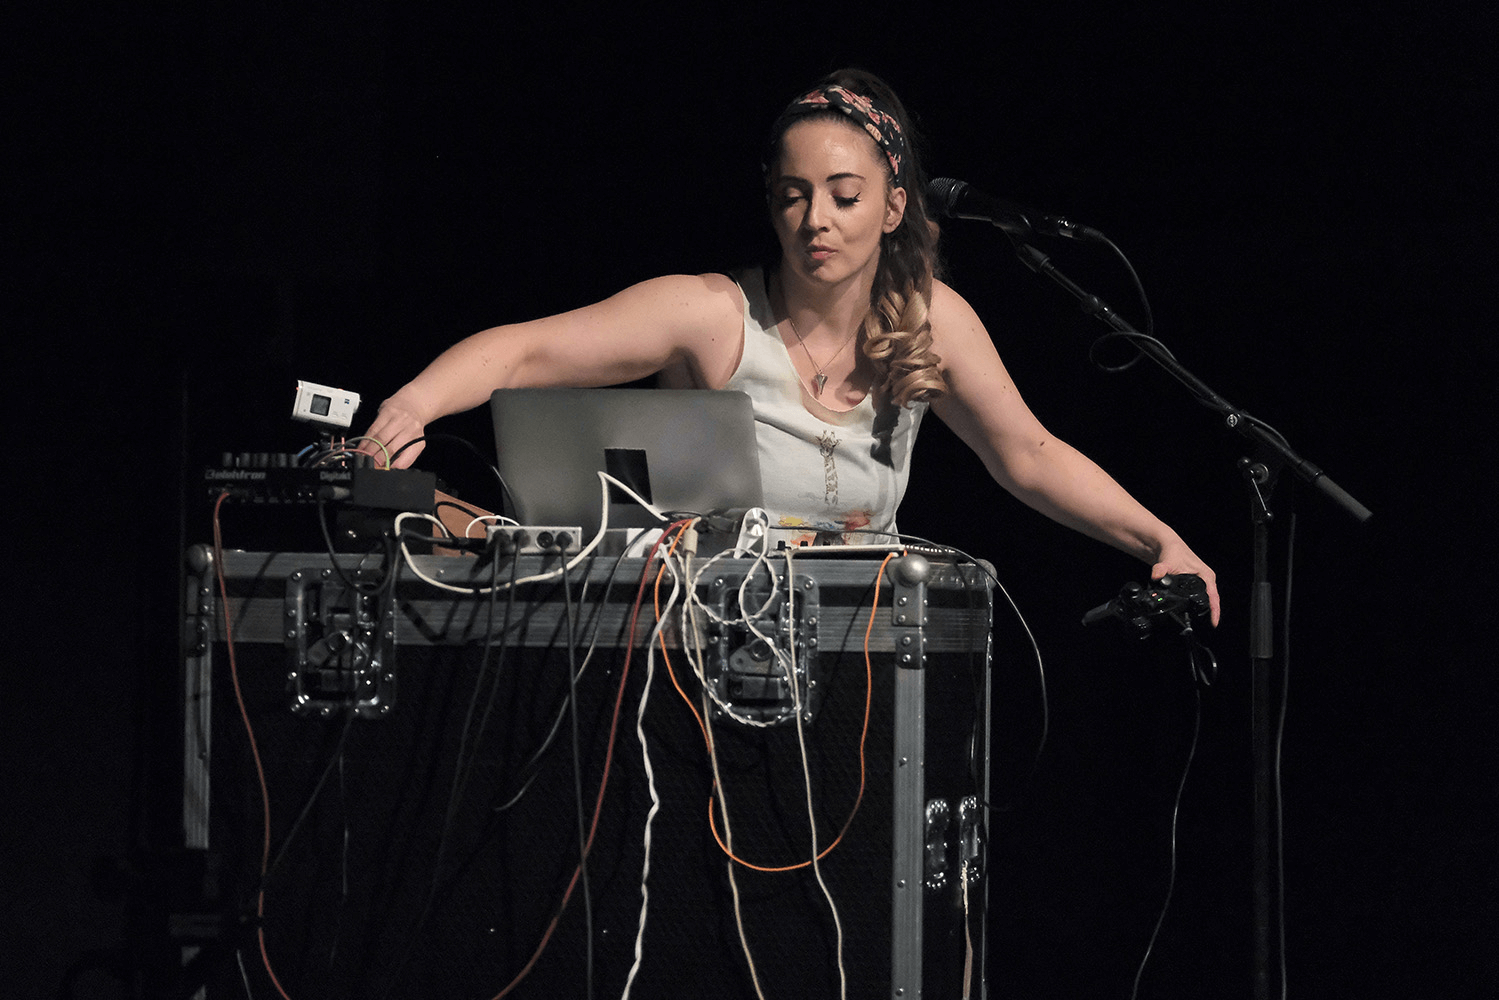
\includegraphics[width=\linewidth]{03-theory/hayes2019.png}
        \captionsetup{justification=justified}
        \caption{\textit{Moon via Spirit} by Lauren Sarah Hayes in performance \citep[taken by][]{slater2019}}\label{fig: slater2019}
    \end{minipage}
\end{wrapfigure}

Lauren Sarah Hayes' work approaches live electronic music practice from an enactive and embodied perspective. This work often uses tangible and haptic controllers that provide non-linear controller input to various elements of the `ecological network of sound analysis and digital signal processing' that constitutes her performance ecosystems. For Hayes, designing complex and adaptive musical systems allows `elements of instability, vulnerability, unpredictability [to] become fodder for the improviser' \citep[p. 2]{hayes2018}. Hayes' creative and research practice has enabled a pedagogical methodology, in which `music and movement-based improvisational practices' are explored in classes of undergraduate students. Through a combination of deep listening methods, movement exercises, and free improvisational exercises, Hayes argues that there is a potential for co-creation of compelling improvisational performances in classes of up to thirty untrained improvisers. These techniques result not only in the active exploration of musical sensorimotor contingencies, but also in the creation of musical meaning that is `brought forth through an emergent extended cognitive network that involves complex relationships between the improvisers involved, technology, and the space in which the performer-instrument pairings are distributed' \citep[p. 8]{hayes2019}. These ensemble improvisations draw from a wide variety of media formats including \gls{ar}. Pointing towards the following assertion by Schiavio and van der Schyff \citeyearpar{schiavio2018}, Hayes notes that digital musical instrument practice ought to develop and augment improvisational practices `that build collectively on individual musical and creative sociocultural histories that individuals bring to the table':
\begin{quote}
    `If the body plays a key role in determining musical learning, so does the socio-material and cultural environment in which it is embedded. However, these dimensions are not separated from the body. Rather, they become manifest through the body and are co-determined by actions and interactions with other bodies and things in socio-culturally meaningful contexts.' \citep[p. 9]{hayes2018}
\end{quote}

\begin{wrapfigure}{l}{0.45\textwidth}
    \vspace{-\intextsep}
\begin{minipage}{0.95\linewidth}
    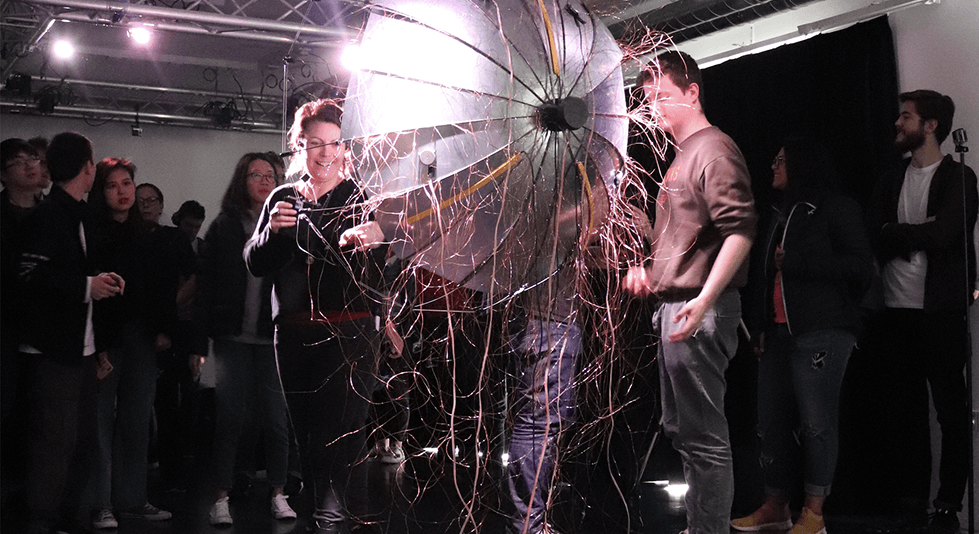
\includegraphics[width=\linewidth]{03-theory/chevalier2019.png}
    \captionsetup{justification=justified}
    \caption{Multiple participants engage with Listening Mirrors \citep[from][]{chevalier2019}}\label{fig: chevalier2019}
\end{minipage}
\hfill
\end{wrapfigure}

Chevalier and Kiefer propose a similar method of promoting musical expression in their \gls{aar} work `Listening Mirrors' \citeyearpar[]{chevalier2018}. Their is system is `audience participation dependent`, and could constitute a realisational \gls{dmi}. Through real-time analysis and re-projection of participants' breath and vocal sounds via bone-conduction headphones and a transducer-augmented parabolic mirror, audience members, environment, and interfaces `feed off each other`, co-creating physical and virtual sound environments that overlap and co-construct a shared hybrid listening space. Their creative and research practice is situated in the later work of Merleau-Ponty and related theories of enactivism. In particular, Chevalier draws from Merleau-Ponty's notion of the `flesh':
\begin{quote}
    `In defining what is meant by `flesh', Merleau-Ponty states, `[w]e must seek space and its content together', that we are `interwoven into a single fabric', a `universal flesh', and `he who sees cannot possess the visible unless he is possessed by it, unless he is of it'. The notion of `flesh', therefore, is both the `flesh of the world' and the `flesh of the body', the relation of the corps sauvage and cultural world and its representations.' (\citeauthor[p. 58]{chevalier2016}, \citeyearpar{chevalier2016}  citing \citeauthor{merleau-ponty1945}, \citeyearpar{merleau-ponty1945,merleau-ponty1968})
\end{quote}

Thus, depending on the specific artwork, from any or each of the \gls{dmi} designer's \citep[]{essl2006,armstrong2006}, improvisational performer's \citep[]{hayes2019}, or installation artist's \citep[]{chevalier2018} perspective, if the material composition of the system with which they are engaging is designed to provide a realisational, dynamic interaction then it `assumes open-ended, fluid, and at least partly indeterminate processes of signification, and as such requires the ongoing cognitive involvement of the musician' \citep[p. 48]{armstrong2006}. This necessity of engagement aesthetically situates such artworks and instruments closer to the site of everyday embodied life, what Dewey terms the return of art to its `origin and operation' in experience. These examples also align themselves with the \gls{4ec} approach to experience, which argues that cognitive process are embodied, embedded, enacted, and extended, across a distribution of mind - body - environment. Readers interested a more comprehensive theoretical and scientific investigation of dynamical systems, embodiment, and computer music artefacts may be interested in David Pirr\`o's thesis, `Composing Interactions' \citeyearpar{pirro2017}.

Augmented reality, specifically due to its ability to mediate perception in real-time and across a multitude of sensory modalities, presents the opportunity to `experiment with, modulate and disrupt [conditions of situated-ness, timeliness, emergence, multimodality and engagement inherent to our embodied coupling] to create new audience collective experiences' \citep[]{chevalier2018}



% --------------------------------------------------------------------------- %
\section{Enactivist Approaches to the Body in XR Systems}\label{sec: theory-embodiment}
We started this chapter with an examination of John Dewey's account of the separation of art from everyday life, and the effect on it thereof. To account for the notion of an aesthetic experience in the appreciation of artistic works, Dewey points towards the `live creature'. This concept, as discussed, contributed to the modern study of \gls{4ec}: the notion that cognitive processes ought to be thought of as embodied, embedded, enactive, and extended across the distribution of brain-body-environment. The previous section outlined my approach to material composition from an artists perspective. The medium of \gls{ar} may be thought of as an `performance ecosystem constituted of relationships between real and virtual processes'. The present section moves forward to consider the experience of participants in such artworks.

%[ ] check \clearpage
\subsection{Embodiment and Enactivism in VR}\label{sec: theory-embodimentvr}
Considerable amounts of research related to embodiment in the context of \glspl{ve} generally falls under specific but necessary discussions and measurements of particular cognitive and affective processes such as presence, emotion, awareness, and consciousness \citep[]{slater1994,seth2012}, for example, in body swap experiments \citep[]{slater2010}, the rubber-hand illusion \citep[]{suzuki2013}, and stimulating altered visual phenomenology \citep[]{suzuki2017}, as shown in \autoref{fig: suzuki2017}. Integration of explicitly \gls{4ec} approaches to \glspl{ve} / \gls{vr} have only started to appear in research in the last 10 years, and is generally lacking from the discourse around \gls{ar}. For example, through an two and a half year autoethnographic exploration of her own experience in the popular \gls{ve} Second Life, Maeva Veerapen integrated the phenomenological theories of Merleau-Ponty and Husserl to analyse and explicate the specific location of `embodiment' inherent in the connection to her virtual avatar. She surmised that `such an experience is still anchored within the user's physical body and that its relation with the avatar's body creates the link between the two spaces, physical and virtual' and termed this state of being \textit{symbembodiment} - symbiotic embodiment of a combined real and virtual self \citep[]{veerapen2011}. 
\begin{wrapfigure}{r}{0.45\textwidth}
    \hfill
    \begin{minipage}{0.95\linewidth}
        \includegraphics[width=\linewidth]{03-theory/suzuki2017.png}
        \captionsetup{justification=justified}
        \caption{Google DeepDream providing (non-realtime) altered visual phenomenology of Sussex campus via VR playback \citep[from][]{suzuki2017a}}\label{fig: suzuki2017}
    \end{minipage}
\end{wrapfigure}

Drawing on Veerapen's notion of \textit{symbembodiment} and linking it to an enactivist approach (indeed, as Varela, Thompson, and Rosch state in their `The Embodied Mind', Merleau-Ponty and Husserl's theories form part of the Western phenomenological roots of their approach \citeyearpar[pp. 173, 18]{varela1993}), Willans et al. argue that the `episodes of emotion' in the experience of \glspl{ve} are linked with feelings of `presence', which in turn emerges from the embedded nature of a participants sensorimotor structure, or, we might say, enaction \citeyearpar[p. 23]{willans2016}. Hovhannisyan et al. argue for an enactivist approach to understanding participant flow, which is motivated by the authors' resistance to the physicalist approach to designing `object-centred'  \gls{vr} experiences that is typically employed \citeyearpar[p. 1]{hovhannisyan2019}. In particular, they turn attention towards what they call an action-predicated perspective (one that focuses on the enactivist theory of perceptually guided action) that they state is `non-reductive with respect to subjective experience', and honours `the pragmatic dimension of perceptual reality' \citeyearpar[p. 18]{hovhannisyan2019}. 

\subsection{Embodiment and Enactivism in AR}\label{sec: theory-embodimentar}
Within \gls{ar}, Riva et al. propose that \gls{ar} and \gls{vr} can transform our `external experience' through the increased levels of presence and engagement they afford, that in turn generates `personal efficacy and self-reflectiveness' \citeyearpar[p. 10]{riva2016}, they further propose that it has the potential to do the same for our `internal experience' . For the authors, `bodily self-consciousness' can be enhanced and extended by altering/extending its boundaries through a process called 'augmented embodiment' , which builds on the hypothesis that embodiment could be altered, expanded, and distributed through \gls{ar} technology: 
\begin{quote}
    `Whenever computer-based information is blended with the perception of the surrounding physical world, as in augmented reality this may become integrated into a new form of altered embodiment. But that requires that the augmentation of the physical with the virtual be carried out in such a way that the user has the potential to feel present. Given the clear popularity of mobility and social connectivity, it seems that presence will increasingly be experienced through attention to an external world in which the physical and the virtual are somehow blended' \citep[]{waterworth2014}
\end{quote}
From an \gls{4ec} approach, `feeling present' in the context of bodily `mobility and social connectivity', emerges, and could be seen to be somewhat analogous with, the notion of action (and other cognitive processes) being embedded in the  socio-cultural and -material norms and values of a participant's environment, their inherent sensorimotor embodiment, and as a result, the propensity for their actions to be perceptually guided (enaction). Suzuki et al. operationalise Nöe's \citeyearpar[]{noe2004} concept of sensorimotor contingencies, as further developed by Seth in the field of predictive processing \citeyearpar[]{seth2014}, by using \gls{ar}/\gls{vr} technology as a test-bed for exploring the effect of modulated sensorimotor contingency and congruency in participant's visual experience of familiar and unfamiliar 3D objects \citep[]{suzuki2019}. Their results indicate that `that the contingency, but not the congruency, of a person's actions and their visual consequences influences access to visual awareness', providing support for a \gls{4ec}-like perspective on perception (and also hinting at the ability for \gls{ar} technology to be used as a method for purposeful sensory illusion through sensorimotor incongruence). Most recently, Chalmers has argued that \gls{ar} has the potential to extend our mind in a more seamless fashion, in a way that he likens to Heidegger's proposal of the `ready-to-hand' nature of certain tools; in use they become an extension of our body without our having to `think' about them and the actions they afford.
\begin{quote}
    `What sort of mental processes do augmented reality devices extend? For a start, they can more seamlessly extend all the processes that smartphones extend: memory (remembering someone's birthday), navigation (getting to the museum), decision-making (deciding where to eat), communication (talking to friends), language processing (translating from another language), and more. But their immersive connection to our perceptual system provides new avenues for extension' \citep[p. 299]{chalmers2022}
\end{quote}
Chalmers further proposes that \gls{ar} provides the grounds for further cognitive extension: our abilities of perception (e.g. through infra-red sensing), recognition (through algorithmic processing and machine learning of real-time environmental data), and imagination (through real-time replacement or transformation of physical objects with virtual ones). Considering Ishi and Omar, -- Inga and Otto's 21st century counterparts -- in \autoref{fig: chalmers2022_2}, Chalmers shows that \gls{ar} devices can theoretically provide cognitive extension, vis-a-vis `The Extended Mind'.

\begin{figure}[ht]
    \centering
    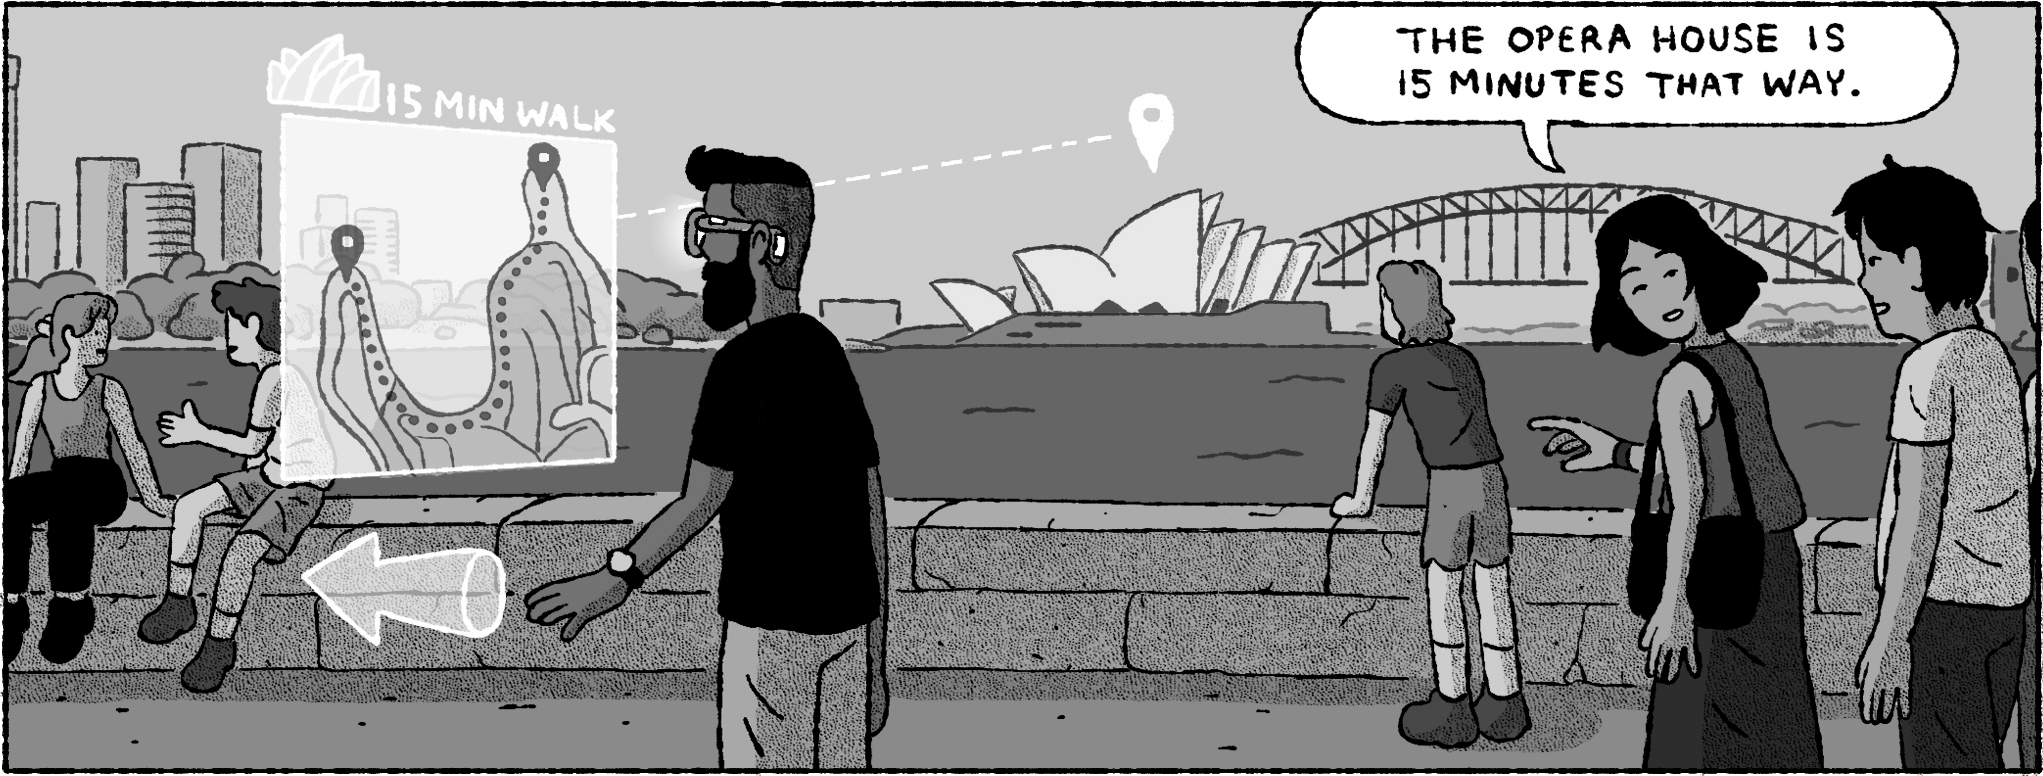
\includegraphics[width=1\linewidth]{03-theory/chalmers2022_2.png}
    \captionsetup{justification=centering,margin=1.5cm}
    \caption{Ishi and Omar on their individually recollected routes to the Sydney Opera House \citep[by Tim Peacock, in][]{chalmers2022}}\label{fig: chalmers2022_2}
\end{figure}



% --------------------------------------------------------------------------- %
\section{The Elephant in Our Headsets: The Zuckerverse}\label{sec: theory-space}
As we have established so far, \gls{ar}, when applied as a medium for the composition, performance, and expression of multisensory art and music, has the potential to:
\begin{enumerate}
    \item Provide new modes of instrumental performance and expression to performers and participants
    \item Radically modulate the embodied experience of performers and participants
    \item Scaffold new musical and artistic meaning through these augmented aesthetic experiences
\end{enumerate}
It follows that such experiences appropriate existing physically real spaces to do so, whilst either (a) simultaneously creating a relational virtual space dependent on the content of the experience, or (b) appropriating physically real spaces to the ends of constructing an entirely new hybrid \gls{ar} space that is greater than the sum of its physical and virtual counterparts. In current popular culture, this notion of a type of physical and virtual hybrid space has been given the term (the) `Metaverse'.

`The Metaverse' gained popularity as a term partway through this writing thesis, partly due to Facebook's calculated re-brand to Meta, partly due to the resulting `bull' run in `metaverse' cryptocurrencies, and partly due to the large subsequent increase of venture capital funding in \gls{xr} start-ups. The reality is however that it is not a new term, having originated from Neal Stephenson's \textit{Snow Crash} \citep[]{stephenson1992}, a sci-fi novel detailing an anarcho-capitalist future in which a \gls{vr}-based internet (The Metaverse) has become the gamified site of socio-cultural and economic norms, values, and interactions. In textit{Snow Crash}, Metaverse users immerse themselves via personal or publicly available terminals (see \gls{vr}), although using public terminals has a negative affect on your avatar appearance and thus your status in The Metaverse.

Though perhaps tangential to, rather than aligned with, the motivations and political thought contained in Stephenson's work, \textit{Snow Crash}, and other novels by him, have influenced Silicon Valley tech oligarchs such as Bill Gates (Microsoft), Jeff Bezos (Amazon), Sergey Brin (Google), John Carmack (Oculus, now owned by Facebook), and Peter Thiel (PayPal, and first external funder of Facebook) \citep[]{rogers2021}. One of the auxiliary aims of this chapter is to ask, `with regards to the unfolding corporate metaverse, is theirs a morally just pursuit?' mainly through the question `should we be willing immersants of their techno(dys/u)topian dream?'. Broadly speaking, the definition of `the' Metaverse has since expanded to contain any sufficiently `immersive web3.0' interaction or \gls{xr} experience. As sound-artists and musicians, this necessarily ushers \textbf{any} \gls{ar} experience we may be composing, performing, or developing under the umbrella term `Metaverse'. Hence, we ought to be aware of the `landscape' so to speak. Do we want our artwork to be associated with this space, or is it tangential to our aims and desires as artists?

Most of these amalgamated definitions are still based in techno(dys/u)utopian ideals of the cybernetic man. This isn't surprising; the technologies the Metaverse makes use of, (\gls{ar}, \gls{vr}, \gls{satnav}) lie `deep within the military and Western - scientific - industrial - patriarchal complex' \citep{davies2004}. A result of this is a paradigm that is also found in \textit{Snow Crash}: the unregulated (see neoliberalism) pursuit of acquiring or constructing virtual `land' or commodities only then to rent/sell it to either smaller corporations, or directly to the individual's drive for commodity accumulation through property and material ownership. This is a needless relationship and is already enacted in the present-day `metaverse', and it is helped by the appropriation of \gls{xr} development and experiences as a `use case' or `value proposition' for Blockchain and cryptocurrency:
\begin{quote}
    `[Living in the metaverse means] having a place to call home, where you can show off your possessions and maybe even have friends over' (own emphasis) \citep[]{marr2022}
\end{quote}
As mentioned in \autoref{sec: theory-experience}, cryptocurrency, and \glspl{nft} are the current landscape on which, more broadly, digital art is being appropriated to increase the price of cryptocurrencies -- through rare artworks, in-game item collectibles, and limited-edition music albums. It is the specific method of artificial scarcity to achieve wealth procurement that is needless. Even in non-crypto Metaverse spaces, the key holders tend to be large corporations, Facebook for example. Unfortunate as this all may be for us `consumers', it is for the betterment of the bottom line of tech oligarchs, and early cryptocurrency adopters - and there must be business as usual. As artists it has fallen to us to propose alternative routes to accessible, diverse, and meaningful digital experiences to catalyse social change.

But the wider implications are even more astounding, beyond the dissemination and consumption of artistic works, even Stephenson's version of `Metaverse' is already here, vis-à-vis virtual land ownership. Many argue it started with Second Life in 2003, but today, cryptocurrency projects like Decentraland, Sandbox, and Somnium Space, as well as corporate efforts like Meta Horizon Worlds, Workrooms, and Home (by Facebook) are the logical conclusions of those early progenitor \glspl{ve}, when it is taken into consideration the lack of regulation around `Big-Tech' and cryptocurrency platforms in general:
\begin{quote}
    `Republic Realm [now Everyrealm] paid a record \$4.3 million for land in the largest metaverse real estate platform, Sandbox. The company is developing 100 islands, called Fantasy Islands, with their own villas and a related market of boats and jet skis. Ninety of the islands sold on the first day for \$15,000 each and some are now listed for resale for more than \$100,000.' \citep[]{frank2022}
\end{quote}

\begin{wrapfigure}{L}{0.45\textwidth}
    \vspace{-\intextsep}
    \begin{minipage}{0.95\linewidth}
        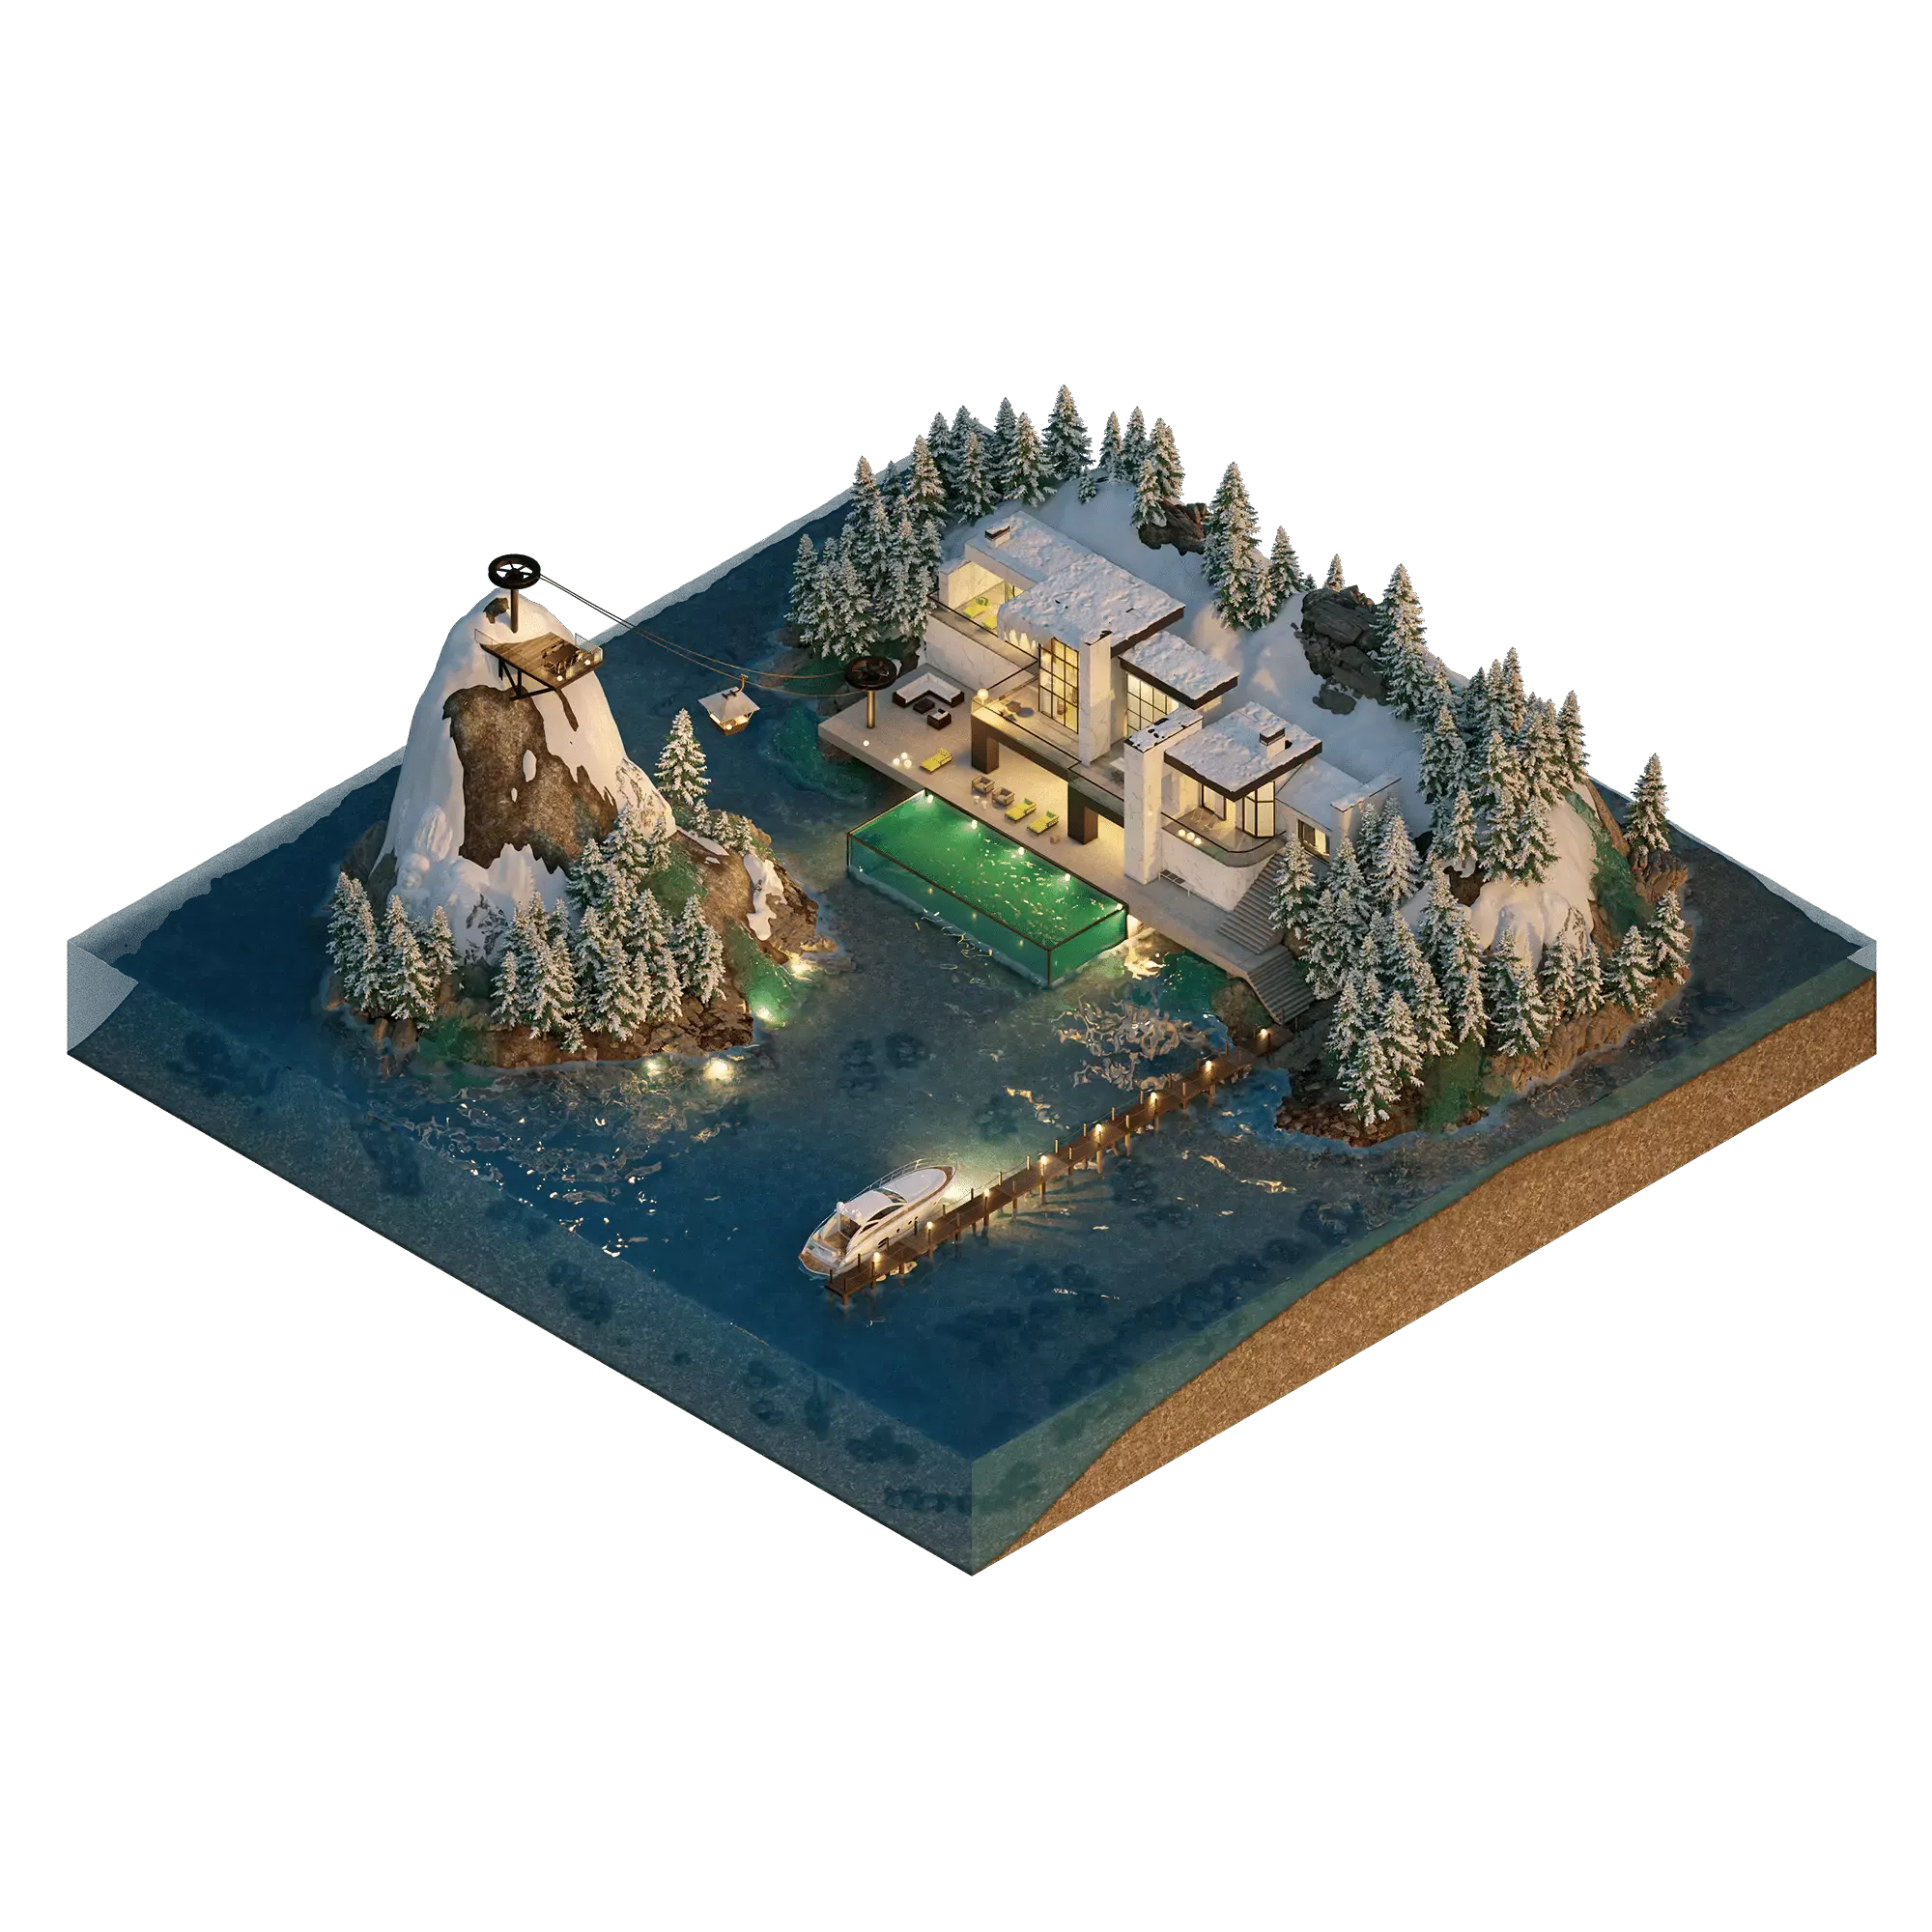
\includegraphics[width=\linewidth]{03-theory/everyrealm2022.png}
        \captionsetup{justification=justified}
        \caption{An example of a rare \textit{Fantasy Island} NFT \citep[from][]{everyrealm2022}}\label{fig: everyrealm2022}
    \end{minipage}
    \hfill
\end{wrapfigure}

This article also mentions that despite \$500,000,000 having been spent in 2021 on virtual land on platforms like The Sandbox, average land prices have decreased 91\% over the last 9 months since their peak in early December 2021, which occurred 1 month after Republic Realm's purchase of \$4.3 million \citep[]{kane2022}. How much of that `property' was bought by or let to retail investors hoping to become rich off of hard-earned savings, only to see 91\% depreciation in their virtual asset? 

What I hope to highlight in this section is that the `metaverse' is not what it is portrayed as. Its current co-option by (or perhaps origination in) the profit motive inherent to cryptocurrency-based metaverse platforms does not `liberate art', rather can lead to unenjoyable \citep{dejesus2022,delic2022}, exploitative , and hyper-commercialised practices \citep[]{ledesma2021,ongwesojr.2022,gach2022}. My criticism of these platforms is not to say that a diversity of media experiences, hosting a multiplicity of sociocultural narratives, from a variety of voices isn't welcome; rather the opposite. \gls{xr} technologies, \gls{ar} specifically, due to its material and embodied relations, propose a real potential to provide a type of embodied artistic liberation. But as Leddy and Puolakka note on Dewey Aesthetics \autoref{sec: theory-experience}, this liberation will never happen under the unchallenged constraints of the capitalist modus operandi. Thus, for as long as both mega-corporations and cryptocurrency is are drivers for use of `space' in `the Metaverse', it will always mirror these conditions and be inherently flawed. Yet if we are to believe the marketing speak, it is in 'spaces' like these that technology companies foresee cultural production shifting to and flourishing in the next 10 years \citep[]{fatemi2022}. Although nascent in their implementation, and not widely known about, thankfully, mechanisms exist (see the Fediverse) to host \glshyperlink[open-source]{opensource}, federated communities away from the clutches and algorithmic abuse of `Big-Tech'. Until that happens in earnest, it leaves us wondering... \textit{What affect will the `Metaverse' have on the production, consumption, and dissemination of art of all types?}

\begin{figure}[ht]
    \centering
    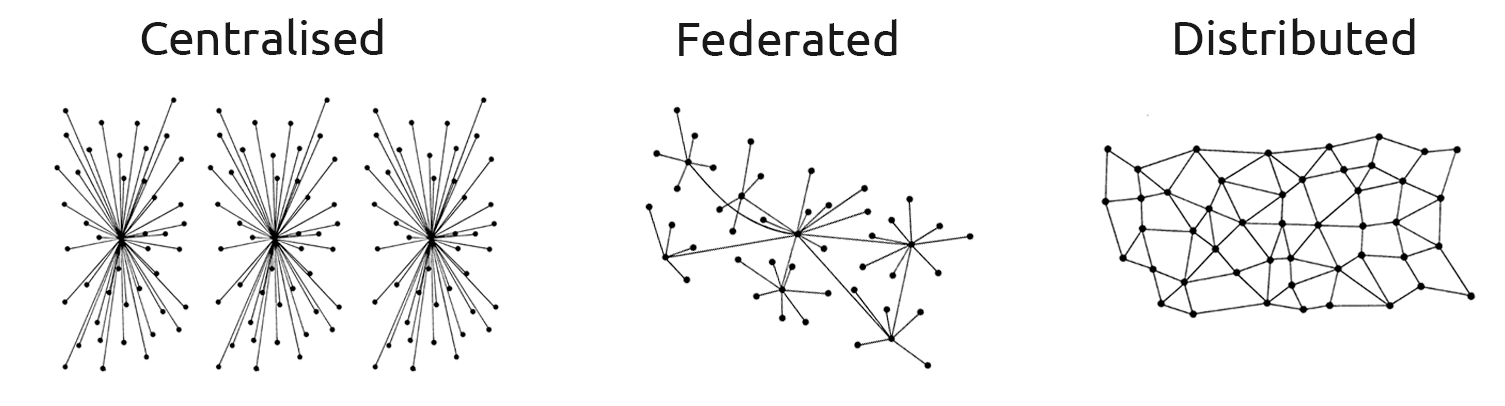
\includegraphics[width=.75\linewidth]{03-theory/baran1964.png}
    \captionsetup{justification=centering,margin=1.5cm}
    \caption{Different communication network types \citep[in][]{baran1964}}\label{fig: baran1964}
\end{figure}


In the next chapter I will outline the approach I have taken in my practice-based research to resist the current conception of `\gls{xr} work \textit{as} the Metaverse'. This includes several forms of resistance, developing a \gls{diy} practice, creating and iterating on openly shared \gls{ar} experiences, and developing a set of design patterns to aid artists and musicians in employing \gls{ar} as a medium for creating similar work.
  \clearpage% --------------------------------------------------------------------------- %
%      _ _                                                _       _           %
%   __| (_)_   _    __ _ _ __  _ __  _ __ ___   __ _  ___| |__   | |_ ___     %
%  / _` | | | | |  / _` | '_ \| '_ \| '__/ _ \ / _` |/ __| '_ \  | __/ _ \    %
% | (_| | | |_| | | (_| | |_) | |_) | | | (_) | (_| | (__| | | | | || (_) |   %
%  \__,_|_|\__, |  \__,_| .__/| .__/|_|  \___/ \__,_|\___|_| |_|  \__\___/    %
%          |___/        |_|   |_|                                             %
%                                                                             %
%                                                    _                        %
%                    __ _ _ __   _ __ ___  _   _ ___(_) ___                   %
%                   / _` | '__| | '_ ` _ \| | | / __| |/ __|                  %
%                  | (_| | |    | | | | | | |_| \__ \ | (__                   %
%                   \__,_|_|    |_| |_| |_|\__,_|___/_|\___|                  %
% --------------------------------------------------------------------------- %
\chapter{A DIY Approach to AR in the Sonic Arts}
\label{sec: method}
\epigraph{\emph{Our environment is not a play, a performance in which only minor modifications are possible. It's an improvisation,[…] the nature of the interaction is radically open.}}{\citep{vermeulen2015}}

\begin{figure}
    \centering
    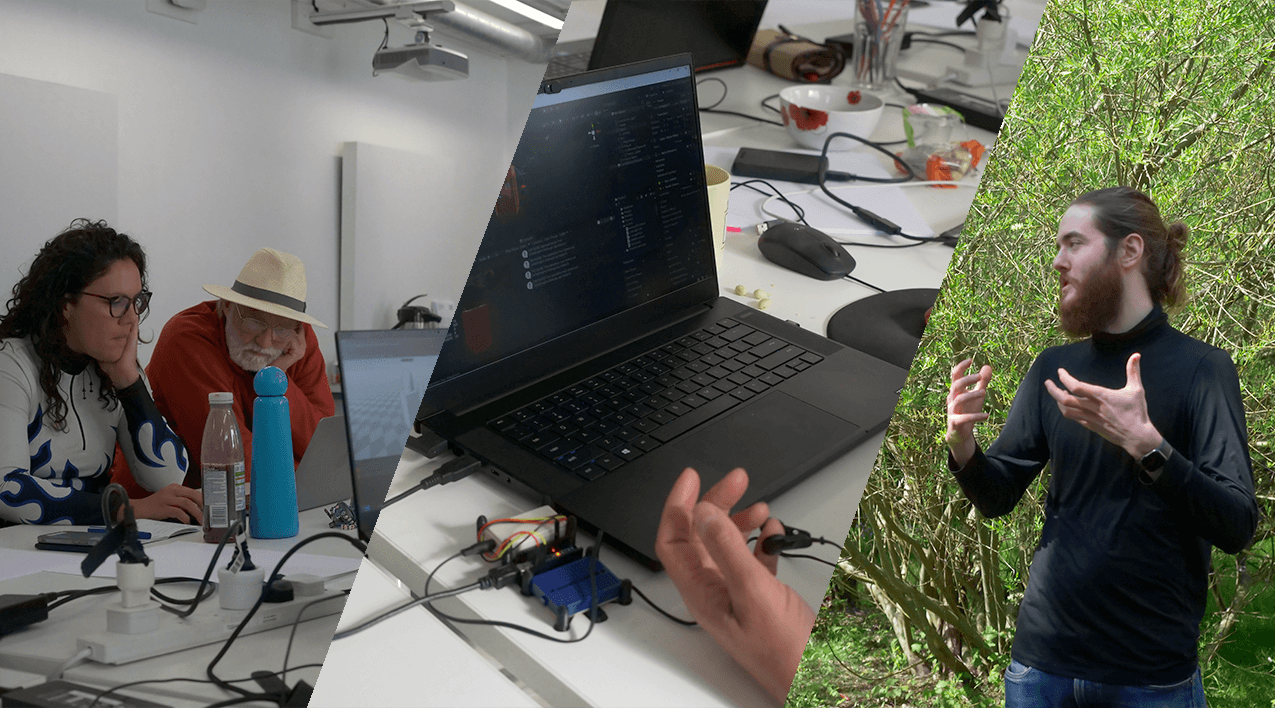
\includegraphics[width=1\linewidth]{04-method/chapter-fig.png}
    \captionsetup{labelformat=empty}
    \caption[\autoref*{sec: method}'s page-figure: Photographs from the Embodiment Hackathon at Sussex, April 30th - May 1st, (from \citeauthor{bonarjee2022}, \citeyear{bonarjee2022})]{}
\end{figure}

\clearpage
% --------------------------------------------------------------------------- %
\section{Summary}\label{sec: method-summary}
In \autoref{sec: review}, the historical origins, contextual trends, exceptions, and contemporary forms of \gls{ar} technologies were outlined. Additionally, examples of \gls{ar}'s use in the arts were provided, along with specific rationales for their use, e.g. sensory engagement, collaborative expression, and activism and agency. A positionality was established that demonstrates that \gls{ar}'s use in the arts is at odds with its origination in military and industrial applications. In the \autoref{sec: theory}, I outlined a trio of lenses through which we may begin to consider the material, embodied, and spatial aspects of sound art using \gls{ar}. In examining complex musical material, it was identified that digital musical systems or `performance ecosystems' offer us fertile conceptual ground for description of material, in the creation and evaluation of rich experiences. The work of researchers approaching experience from an enactivist perspective when working with \gls{xr} technologies was then outlined. Finally, an examination of the current state of the `Metaverse' as a space to describe \gls{xr} experience in general was critiqued. These three lenses all drew from an understanding of art \textit{as} experience, and the disconnection between art and everyday life, an alienation that comes as no surprise given its commodity fetishisation by free-market capitalism. Moreover, the lenses were contextualised within a \gls{4ec} approach to experience, which posits that cognitive processes are embodied, embedded, enacted and extended; inseparable from the brain-body-environment that they constitute and are situated. In the current chapter I will be outlining my methodological approach that has informed both the theoretical, and practical sides of the research: designing, performing, and evaluating sound art \gls{ar} experiences (\textit{sound \gls{art}} to borrow from Rhodes \citeyearpar{rhodes2018}). A review of the outstanding research questions will be outlined, to provide the chapter a clear direction into the ensuing three study chapters.

\begin{enumerate}
    \RQmedium
    \RQexperience
\end{enumerate}

This thesis approaches the above questions by making use of several established practice research methods. Broadly, these methods have led to practical contributions that will be explored in the following three study chapters: 
\begin{itemize}
    \item the creation and iterative design of multisensory sound \gls{art}
    \item a set of open design guidelines for creating similar sound \gls{art} compositions and performances
\end{itemize}
These practical contributions have functioned both as ongoing research probes, and as platforms for open and reproducible artistic work for the wider experimental music research community. The methods present in this thesis have stayed consistent with their original proposal, with the exception of specific methods of data collection and analysis being adapted to suit the restrictions of the COVID-19 pandemic, which commenced three months after the start of research. 

As will be developed on in \autoref{sec: discussion-guidelines}, it is within this context of creating, developing, implementing and iterating on a set of open design guidelines for \gls{ar} art and music that the research methods employed in the following chapters are carried out. This started with a motivation for creating smaller experiences, that were simple in their sensory modulation and instrumental reactivity, with the view to later incorporate them into larger scale interactive \gls{ar} experiences once sufficiently tested. However, due to COVID-19, the prospect of user-testing and iterating on the design of multiple experiences, especially large scale ones, through participant feedback became increasingly difficult to facilitate and plan for. Thus, I opted to focus on developing working sound art \gls{ar} prototypes that I myself would compose with regularly, tweak, and iterate upon. Then, and there, an \gls{ar} research and compositional practice began.

It is pertinent to mention that practical work, where carried out, has always been documented for analysis, open-research, and archival purposes. I found the combination of \href{https://sambilbow.github.io}{my personal website} as well as \href{https://github.com/sambilbow}{GitHub} and \href{https://youtube.com/@sambilbow}{YouTube} a suitable and cost-effective solution for this. Links to project files will be included in the study chapters, and cited websites have been archived using \rurl{archive.today} \footnote{\url{https://en.wikipedia.org/wiki/Archive.today}}. Before outlining the specific methods touched on in later chapters, I would first like to touch upon the concept of resistance, and its role in motivating the methodological approach taken in the thesis.



% --------------------------------------------------------------------------- %
\section{Resistance in Practice}\label{sec: method-resistance}
Formative in the development of the methodological approach of this thesis has been the concept of `resistance'. In short, this could be characterised as a motivation for changing or acting against the state of the art, practice, technology, or philosophy, out of a discontent for its status quo. This isn't to be confused by resistance in the sense of experiencing resistance to \textit{do} something, although as might be expected, that has reared its head a few times over the last three years too. It is difficult to place resistance into the linear narrative of this text; some resistance formed my initial motivations for the carrying out of this research, and some was garnered along the way, especially around the time of the unfortunate uptake in `Metaverse' as a term to describe the sum total of all creative \gls{xr} development and labour. Either way, resistance has made up a large portion of my approach to \gls{ar} technologies, its role within digital music and humanities more broadly. These forms of resistance can be separated into three main categories.

\subsection{AR as Consumer Technology}\label{sec: method-resistance-maker}
As referred to in \autoref{sec: theory-experience}, contemporary design research in the fields of computational art and music have in recent years rallied behind the broader \gls{floss} and \gls{osh} ethoses. This approach, often hand-in-hand with the Maker, \gls{diy}, and Hardware Hacking subcultures, stands in stark contrast to the goings-on of mega-corporations board rooms, with their design `sprints', `agile' workflows, and `human (customer)-centred' design. The approaches taken by these subcultures towards embodied design and composition workflows however, has been highly beneficial for the field. In the case of digital music making, software, hardware, and live-coding tools like \gls{pd}, Maximilian, Supercollider, ixilang, Sonic Pi, TidalCycles, FluCoMa, and Bela have granted students, researchers, and composers across disciplines, free and beginner-friendly access to a wealth of software tutorials, examples, and tools for advanced real-time sampling and synthesis techniques.

It could be proposed, that this approach is motivated in part by a resistance against many of the `features' typically found in commercial `closed-source' software and hardware. Providing significant barriers to accessible learning, creativity, and artistic authenticity, these include lack of interoperability with other software, use of proprietary file formats, high initial or recurring subscription costs, and restricted access to lower-level parameters, functions, and settings. It is within this resistance against the closed-source and / or commercial that the practical work of this thesis attempts to situate itself, drawing on its implicit designerly practices and aesthetics. As a result, the path taken to address the key areas of the thesis has involved the bringing into the fore, knowledge from the creative practice of hacking, making, designing, and iterating with experimental and \gls{diy} \glshyperlink[open-source]{opensource} \glshyperlink[hardware]{osh} and \glshyperlink[software]{floss}.

While commentary on the considerable role of un(der)funded volunteer labour involved in \glshyperlink[open-source]{opensource} tools and projects is outside of the scope of this thesis, it is worth mentioning. In this way, `\glshyperlink[open-source]{opensource}' is never taken to describe the best way of carrying out a project, rather I hope to convey that the ideals and features of an \glshyperlink[open-source]{opensource} ethic are beneficial to the aims of this thesis, vis-à-vis developing the understanding of new technologies within the \gls{nime} field, and attempting to manoeuvre what is essentially a minefield of technologies that are only available today because of U.S. defence funding.

\subsection{AR as Visual}\label{sec: method-resistance-ocularcentrism}
A second form of resistance that the methodological approach of this thesis explored is the ocularcentrism found in \gls{ar} technologies mentioned previously in \autoref{sec: ar-sensory-visual}. As a practitioner of music, and audio related technologies, this has provided a significant portion of the motivation for carrying out the present research, as well as a significant portion of the challenges faced when attempting to develop \gls{ar} as a medium for sound-based interactive experiences. Developing new interfaces for musical expression invariably leads to the appropriation of technology `not meant' or `not for' musical expression, and this is where \gls{nime} practice has considerable crossover into the maker / \gls{diy} / hardware-hacking subculture. The present thesis approaches ocularcentrism head-on, not through replacing the visual, but through re-ordering, with the aim to even-out, the sensory hierarchy of \gls{ar} technologies. 

Realistically, however, technologies relating to touch, and especially the chemical senses, present significant barriers compared to the visual and auditory senses in terms of access, cost, expertise, and time. In this research I have attempted to make room for future cases where this technology may be available, by using \glshyperlink[open-source]{opensource} \glshyperlink[hardware]{osh} and \glshyperlink[software]{floss} where possible, and by presenting a case for the design of \gls{msar} experience in the set of design guidelines in \autoref{sec: discussion-guidelines}. Thus, the present thesis approaches audiovisual, gestural \gls{ar} as a starting point for my own \gls{ar} composition and performance, with a mindful eye (or ear) to the future capabilities of multisensory \gls{hci} technologies.

\subsection{AR as Overlay}\label{sec: method-resistance-overlay}
The third form of resistance drawn from in the thesis is that of \gls{ar}'s paradigmatic function as an `overlay' device. So far, the origin of this approach, and contemporary alternatives to it have been explored \autoref{sec: ar-process}, with a case being made by practitioners \citep{mann1994,schraffenberger2018,chevalier2020} towards re-situating \gls{ar} as a process of perceptual mediation. In the present research, the resistance towards \gls{ar} functioning as a \gls{hud} has led to propositions on how these approaches intersect with a \gls{4ec} approach to experience, later on, in \autoref{sec: discussion-medium-embodiment}. In practice, it has motivated the \gls{ar} experiences developed in this research to go beyond passively layering sensory stimuli in front of immersants \textit{as experience itself}. This is achieved by presenting experiences that are contingent on immersant movement, gesture, and environmental sounds, not only passive viewership. In this way, the \gls{ar} experience can be thought more of as a hybridisation or alteration of reality rather than an simple \gls{hud} augmentation of reality.

As with multisensory technologies though, technologically achieved `diminished reality' and other non-augmenting subforms are, in general, more computationally expensive and beyond the scope of the research practice due to lack of expertise and time. By way of acknowledging their importance as valid methods of perceptual mediation, they are accounted for in the design guidelines presented in \autoref{sec: discussion-guidelines}.



% --------------------------------------------------------------------------- %
\section{Research in Practice}
The three ensuing chapters, \textit{\nameref{sec: area} (2020)}, \textit{\nameref{sec: polaris} (2021)}, and \textit{\nameref{sec: polygons} (2022)} outline and analyse three \gls{ar} interactive music systems developed over the course of this thesis, each with different but converging focuses. They make up practical contributions to knowledge, as well as forming the grounds for the propositions in \autoref{sec: conclusion}. Though they were initially guided by a loose set of proto-design guidelines \citep{bilbow2020}, it is through the insights and analysis gained in their creation and iteration that the \nameref{sec: discussion-guidelines} in \autoref{sec: discussion} have been developed; they can therefore also be thought of as research probes in their own right.

\textit{area\textasciitilde{}} was the starting point for practical work in the present thesis. It is a non-visual \gls{aar} experience centred around the self-composition of a hybrid listening environment using an ambisonic microphone, head-, and hand-tracking. As will be expanded upon in the next chapter, due to the circumstances of the COVID-19 lockdown, I opted for an \gls{abd} method for the iteration and evaluation of the system. Out of the evaluation of this project, namely the endeavour to expand into \gls{av} \gls{ar} experiences, I discovered a suitable platform the develop the rest of doctoral research on: the \glshyperlink[open-source]{opensource} \gls{pns} \gls{ar} headset. \textit{polaris\textasciitilde{}} describes an \gls{ar} experience that was developed to examine the suitability of the \gls{pns} \gls{ar} headset's use in an \gls{av} installation context. Participant studies were conducted and an evaluation of their experience was carried out via the grounded theory method of analysis. \textit{polygons\textasciitilde{}} was a direct result of sharing the experience of artistic \gls{ar} with the participants of \textit{polaris\textasciitilde{}}. In proposing an Sound \gls{art} Performance Practice, it describes the composition of a set of \gls{ar} musical instruments, technical setup, and considerations of deploying an \gls{ar} headset as a medium for musical performance. Both \textit{polygons\textasciitilde{}} and \textit{polaris\textasciitilde{}} were also developed using the \gls{abd} method, although it was less formally implemented as COVID restrictions lessened and I was able to pilot the technology with friends and colleagues.



  \clearpage% --------------------------------------------------------------------------- %
%                                      _                                      %
%   ___ ___  _ __ ___  _ __   ___  ___(_)_ __   __ _                          %
%  / __/ _ \| '_ ` _ \| '_ \ / _ \/ __| | '_ \ / _` |                         %
% | (_| (_) | | | | | | |_) | (_) \__ \ | | | | (_| |                         %
%  \___\___/|_| |_| |_| .__/ \___/|___/_|_| |_|\__, |                         %
%                     |_|                      |___/                          %
%                                                                             %
%                                                   __ _ _ __ ___  __ _       %
%                                                  / _` | '__/ _ \/ _` | /\/| %
%                                                 | (_| | | |  __/ (_| ||/\/  %
%                                                  \__,_|_|  \___|\__,_|      %
%                                                                             %
% --------------------------------------------------------------------------- %
\chapter{Composing area\textasciitilde{}}{Exploring Real and Virtual Environments Through Gestural Ambisonics and Audio Augmented Reality}
\label{sec: area}
%\markboth{}{Composing area\textasciitilde{}: Exploring Real and Virtual Environments Through Gestural Ambisonics and Audio Augmented Reality}
\epigraph{\emph{}}{}

\noindent \textbf{area\textasciitilde{} Code:}        \url{https://www.github.com/sambilbow/area}

\noindent \textbf{area\textasciitilde{} Guide:}       \url{https://www.github.com/sambilbow/area/wiki}

\noindent \textbf{area\textasciitilde{} Publication } \url{https://doi.org/10.21428/66f840a4.b74711a8}

\clearpage

% --------------------------------------------------------------------------- %}.

%This move has helped democratise the use of AR as a medium, tool, and collaborative technology, allowing the maker community develop tools \citep{rompapas2020} that aid in critiquing the tensions and various relationships between real and virtual environments. Furthermore, it has presented a unique opportunity for computational artists and digital media researchers that want to develop for an AR HMD but either cannot afford to spend £1000-£2500 on one, or cannot justify buying closed-source devices due to clashes in research ethics due the provision of personal data required by parent companies.

\section{Summary} \label{sec: area-summary}
In this chapter, I outline the development and evaluation of the \textit{area\textasciitilde{}} system that I created in 2019 as the initial research probe into sound-driven AR experiences. \textit{area\textasciitilde{}} enables its user to record, manipulate, and spatialise virtual audio samples or nodes around their immediate environment. Through a combination of ambisonics audio rendering and hand articulation tracking, this system calls attention to the ability of non-visual augmented reality (AR), here, audio augmented reality (AAR), to provide new aesthetic experiences of real and virtual environments.
Through an autobiographical design study, these experiences are discussed in relation to the research question: \textit{“How can we better understand relationships between virtual and real environments through gesture and virtually placed audio augmented reality objects?”}. The system is contextualised within the move in computational art, and indeed, broader human computer interaction research, towards multisensory interaction. In particular, \textit{area\textasciitilde{}} is situated in the creative practice of works using multisensory AR as a medium to create expressive computational sound art.

The \textit{area\textasciitilde{}} system is a gestural sound sampler that uses hand and head tracking to place and manipulate virtual audio sources in the user’s environment, heard through bone conduction headphones which transmit sound directly to the cochlear without occluding the their hearing. This allows the them to experience \textit{virtual audio environments} overlaid seamlessly onto the \textit{real audio environment}. Through gesture, they can interact with and shape the combined \textit{real and virtual audio environment} surrounding them.

The three technologies used in \textit{area\textasciitilde{}} are gestural hand tracking, rotational head tracking, and ambisonics. The gestural hand tracker used in the system is a Leap Motion LM-010 Controller \footnote{\url{https://www.ultraleap.com/product/leap-motion-controller/}}, a USB infrared camera device that provides location and orientation data output of individual finger joints (and therefore hands) when they are presented above the device. The Leap Motion Controller (LMC) has been adopted in a multitude of settings such as being mounted on VR headsets \footnote{\url{https://archive.vn/GQtAH}}, and converting hand gestures to MIDI \footnote{\url{https://archive.vn/3M1PX}}. More recently, Ultraleap are investigating the use of this same technology with gesture-based public information screens to help combat the “hygiene risks of touch screens” \citeyearpar{ultraleap2020a}.

Rotational (not positional) head tracking is achieved via an inertial measurement unit (IMU). This small and inexpensive component provides orientational data output at 20 times a second. When affixed to the head via a headset or headphones, it is a relatively easy and cheap way of implementing head tracking into the system.

Ambisonics is an audio format that allows for full-spherical audio capture and playback \citep{gerzon1973}, meaning that it includes sound sources above and below the listener as well as the conventional horizontal plane. There are four recorded channels (referred to as A-Format) that, unlike regular mono, stereo or surround sound formats, contain no information about the speakers that the signal should be delivered to. Rather, these channels can be encoded in such a way as to describe a three-dimensional field of sound referred to as B-Format, allowing the producer or artist to think in terms of sound sources in three dimensions rather than conventional speaker placement. B-Format can be decoded through “virtual microphones”, any number of which can be placed within this three-dimensional sound field to provide standard channel outputs.

For example, in \textit{area\textasciitilde{}}, I have used a RØDE Soundfield NTSF-1 microphone array comprised of 4 microphones. The A-Format output is encoded to B-Format by an audio plugin. A software library decodes the B-Format to two responsive, binaural, virtual audio output channels. This all occurs in real-time, so that the microphones inside the three-dimensional sound field rotate proportionally as the composer moves their head, providing realistic changes to what is heard.



% --------------------------------------------------------------------------- %
\section{Designing \textit{area\textasciitilde{}}} \label{sec: area-system}
The \textit{\textit{area\textasciitilde{}}}  system, which stands loosely for ‘augmented reality environmental audio’ aims to afford its user the ability to spectromorphologically (defined by Smalley to concern spatial, temporal and textural qualities of sound \citeyearpar{smalley1997}) manipulate sounds from their environment into a \textit{virtual audio environment}. Through bone conduction headphones and head tracking, this sound field is heard in synchronicity with their actual environment. The system was created in order to explore and reveal the relationship between real and virtual environments in AAR systems.

%*[ ]   fix figure
\subsection{Hardware Implementation}            \label{sec: area-system-hardware}
\begin{figure}
    \centering
    \subcaptionbox*{}[.45\textwidth]{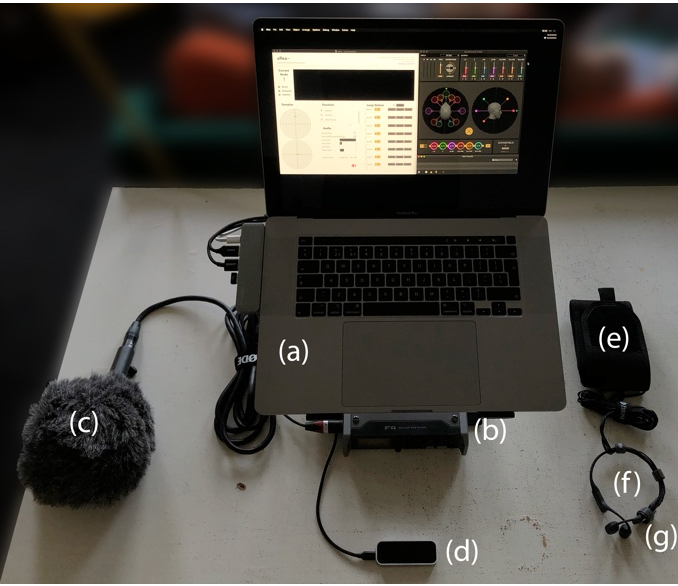
\includegraphics[height=5.5cm]{figures/05-area/areatechnical_hardware.png}}%
    
    \subcaptionbox*{}[.45\textwidth]{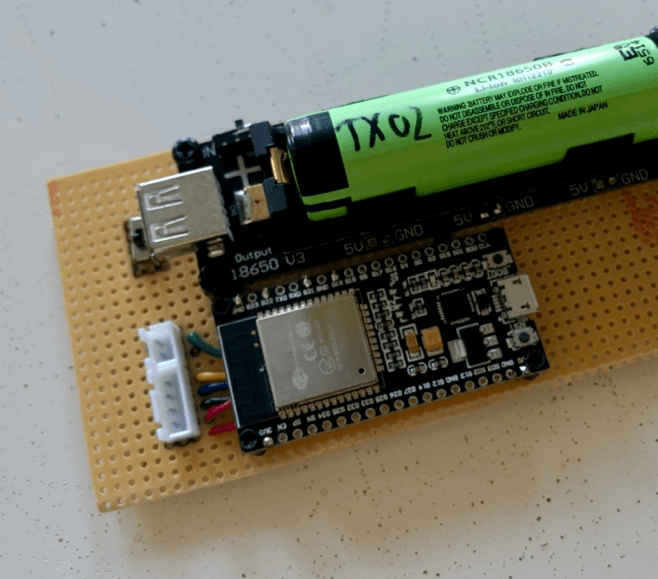
\includegraphics[height=5.5cm]{figures/05-area/areatechnical_pcb.png}}%
    \caption{\textit{area\textasciitilde{}} hardware and PCB}
    \label{fig: areatechnical}
\end{figure}

The on-desk hardware for the \textit{area\textasciitilde{}} system shown in Figure 2 includes (a) a laptop running the Max MSP \footnote{\url{https://cycling74.com/products/max}} patch, (b) a 4 channel input audio interface, (c) an Ambisonic microphone, and (d) a Leap Motion Controller.

The wearable hardware used for the \textit{area\textasciitilde{}} system comprises 2 sections: (e) a belt pouch containing a PCB-mounted ESP32 microcontroller \footnote{\url{https://www.espressif.com/en/products/socs/esp32/overview}} and 18650 battery (shown in \autoref{fig: areatechnical}), and (f) a pair of bone conduction headphones \footnote{\url{https://aftershokz.co.uk/products/aeropex}}, with (g) a mounted inertial measurement unit (IMU) for tracking head orientation. 

The IMU and ESP32 are connected via a detachable 1.5m heat shrunk cable that runs from the back of the bone conduction headphones, down the length of the user's back and into the belt-mounted transmitter pouch. With the integration of an Arduino library \footnote{\url{https://github.com/kriswiner/ESP32/}}, the IMU data is transmitted to the laptop via Bluetooth from the ESP32. Audio is transmitted to the headphones via Bluetooth from the Max MSP patch running on the laptop. 

The only hardware that needs to be accessible for the person composing with \textit{area\textasciitilde{}} is the Leap Motion Controller and the wearable hardware system. The laptop and audio interface are ideally hidden from view so as to minimise distraction. The microphone should be placed in a location that will provide them with access to sounds that they wish to compose with.

\subsection{Software Implementation}            \label{sec: area-system-software}

%*[ ]   fix figure
\begin{figure}
    \centering
    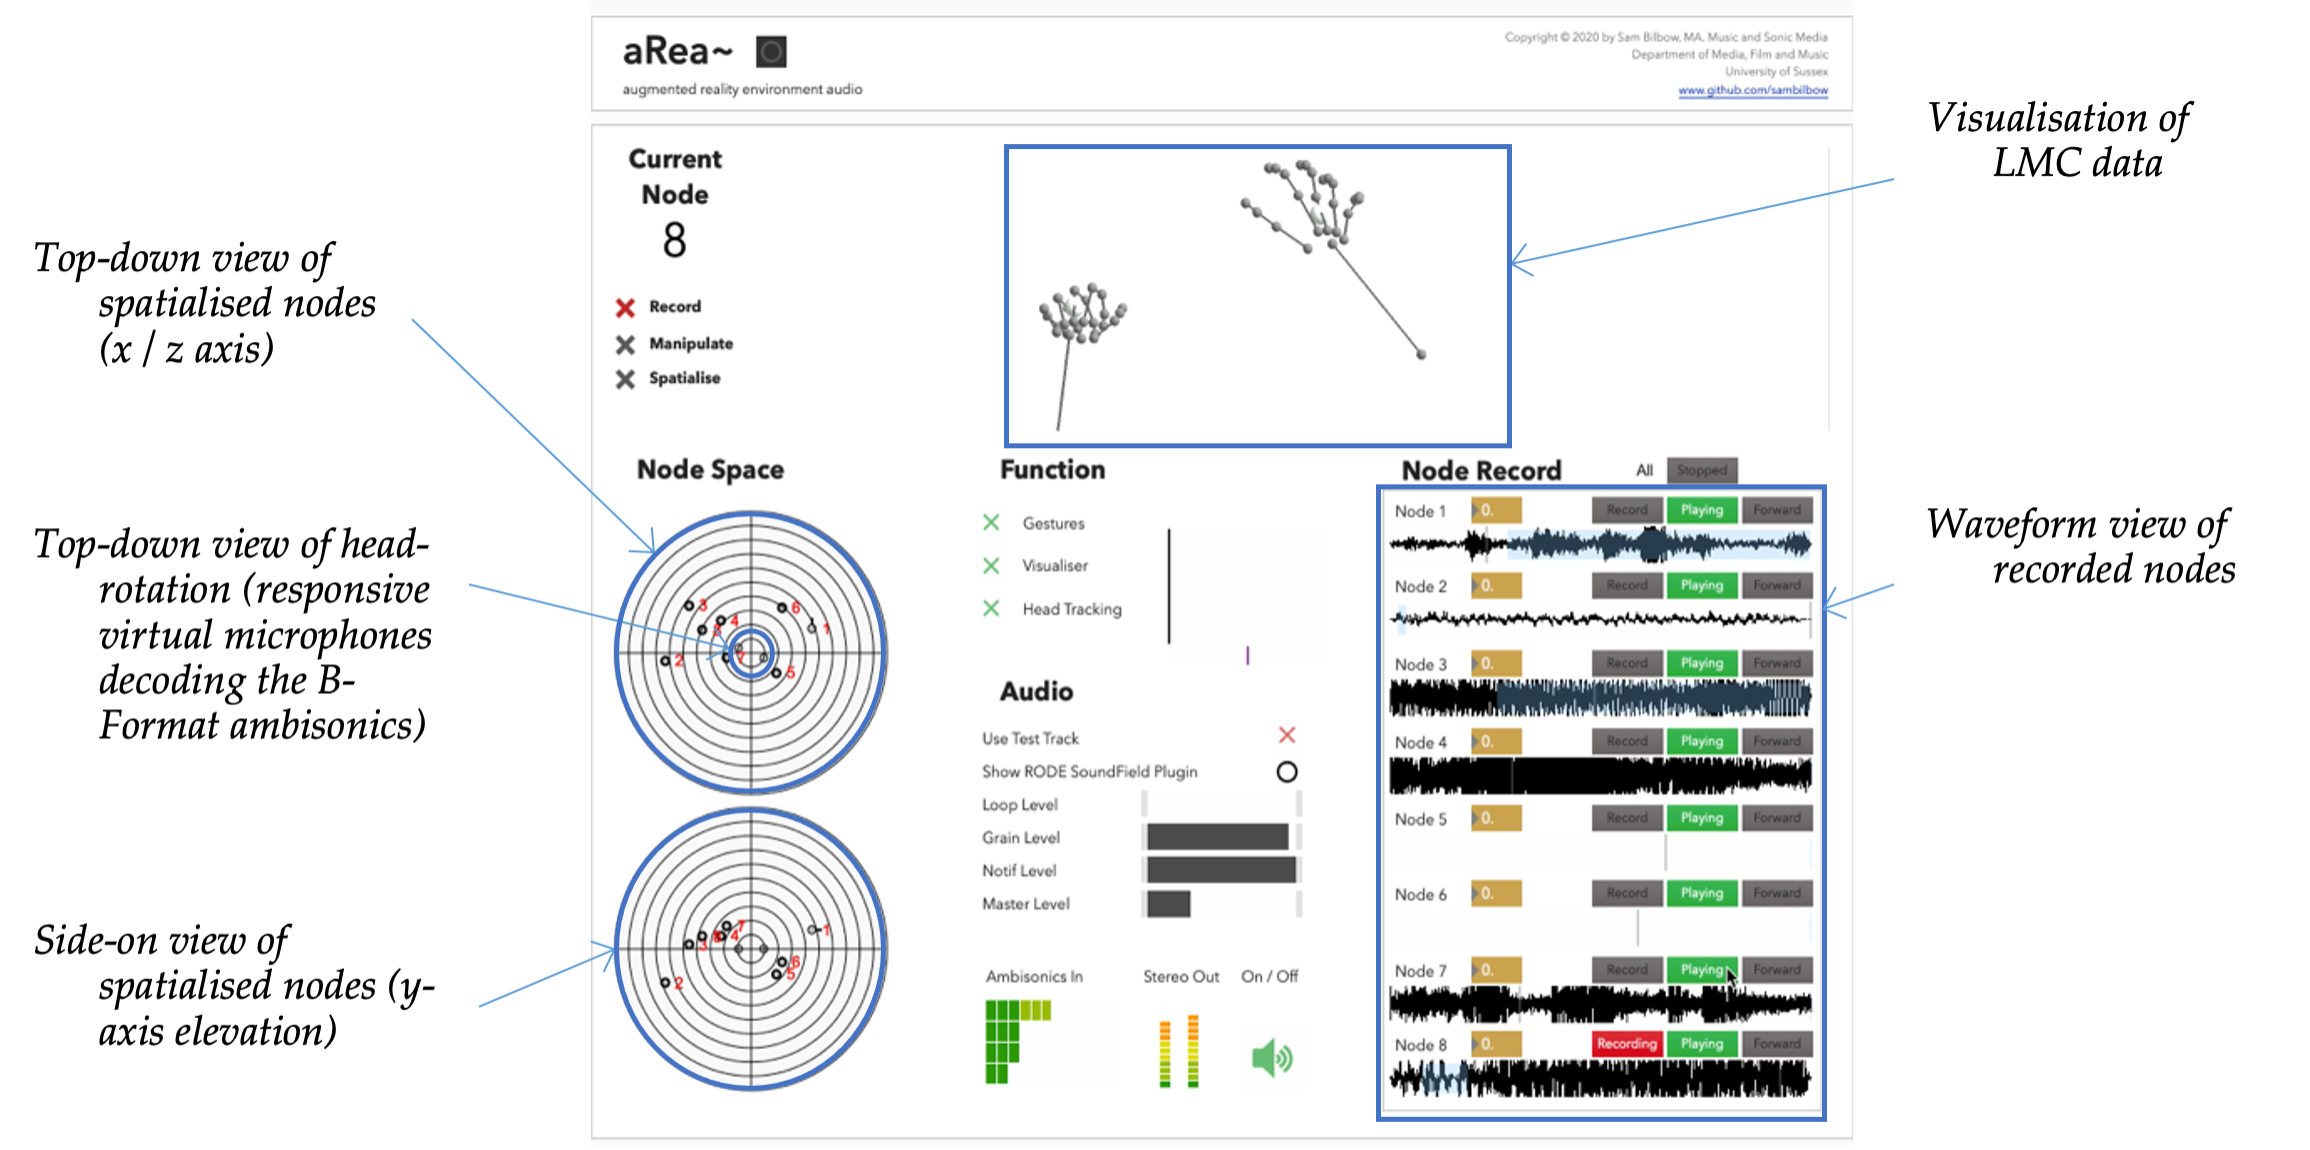
\includegraphics[width=\linewidth]{figures/05-area/areatechnical_max.png}
    \caption{\textit{area\textasciitilde{}} Max MSP patch}
    \label{fig: areatechnicalmax}
\end{figure}
The patch (\autoref{fig: areatechnicalmax}) uses the audio plugin \footnote{\url{https://www.rode.com/soundfieldplugin}} shown in \autoref{fig: areatechnicalrode} to encode the A-Format ambisonics microphone input into B-Format (a three-dimensional sound field), or what I will refer to as the \textit{ambisonic palette}. This \textit{ambisonic palette} is not heard by the composer; instead, they can sculpt from it, forming their own audible \textit{(B-Format) virtual audio environment} through hand gestures. I have defined these gestures in Max MSP with help from the IRCAM Leap Motion library \citeyearpar{ircam2014} \footnote{\url{https://github.com/JulesFrancoise/leapmotion-for-max}}, and they occur over three stages of interaction: \textit{\textbf{record, manipulate, spatialise}}. 

%*[ ]   fix figure
\begin{figure}
    \centering
    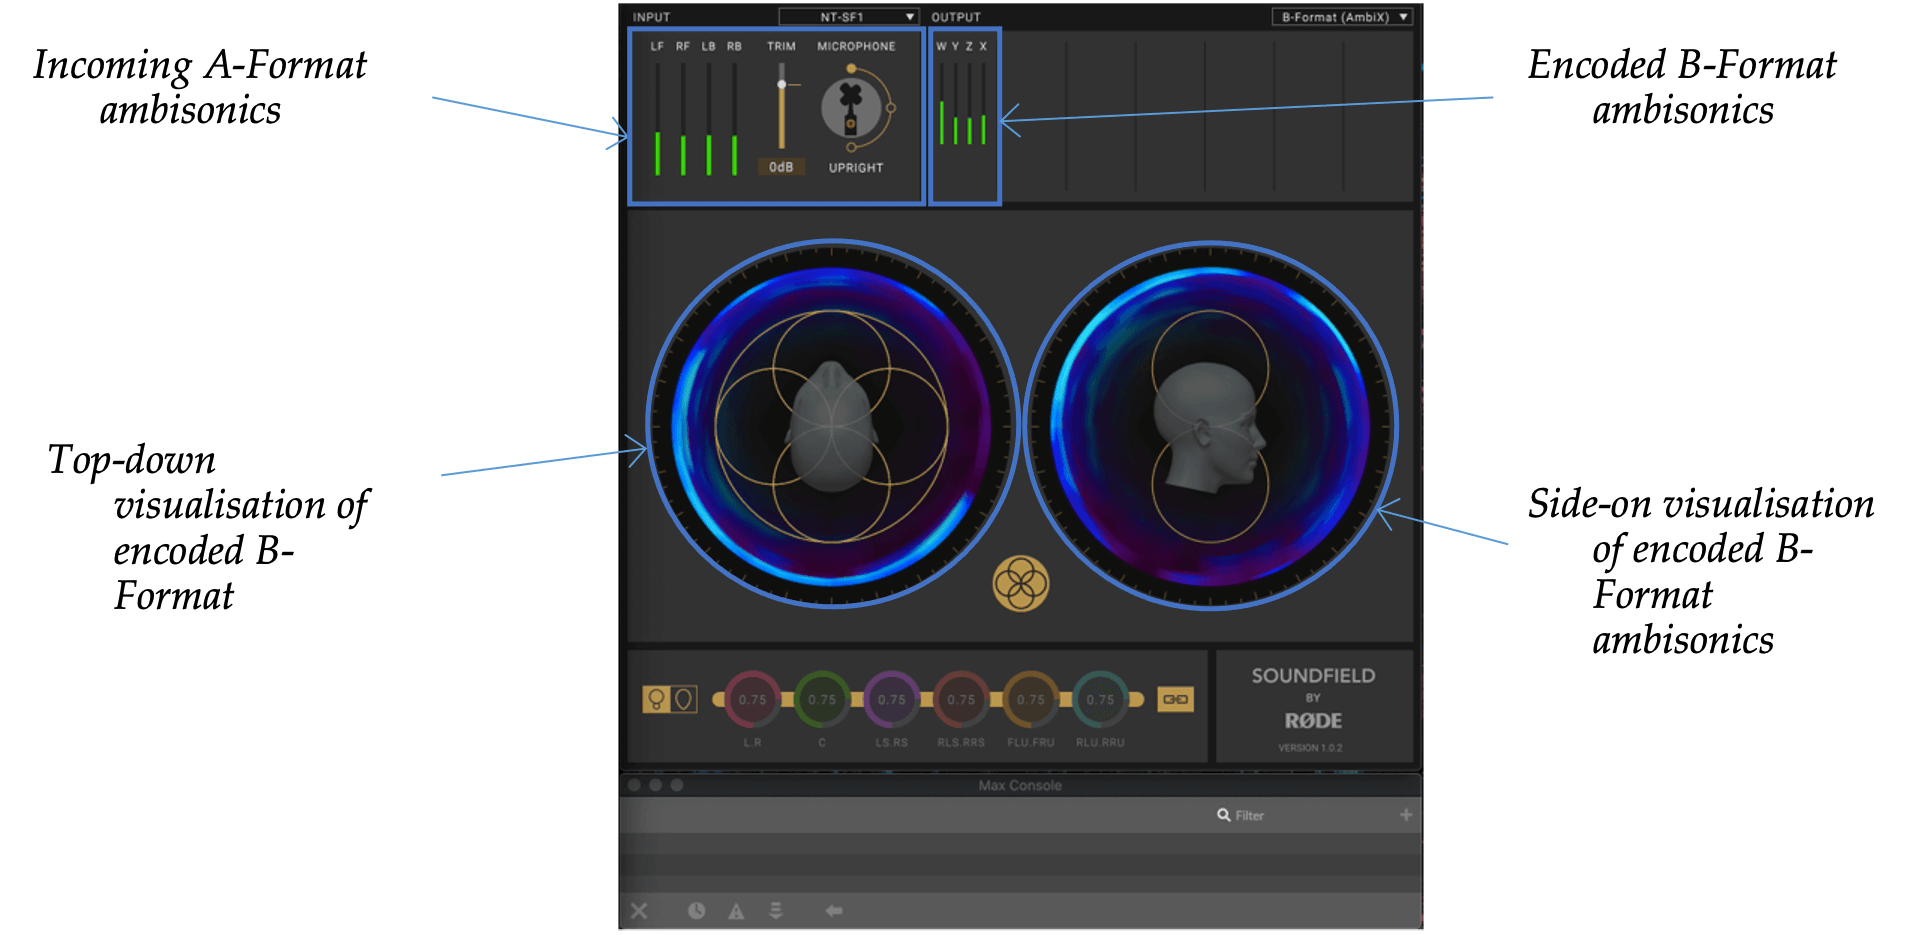
\includegraphics[width=\linewidth]{figures/05-area/areatechnical_rode.png}
    \caption{RØDE Soundfield Plugin}
    \label{fig: areatechnicalrode}
\end{figure}

\subsubsection{Record}                          \label{sec: area-system-software-record}
The \textbf{recording or ‘sampling’ stage} is initiated by making a left-hand grab above the LMC, the longer lasting the grab, the longer the portion of audio from the \textit{ambisonic palette} is sampled. The three-dimensional coordinates of the hand above the LMC correlates with the location of audio recorded (this is achieved by mapping the hand coordinates to a virtual microphone inside the \textit{ambisonic palette}), essentially allowing the composer to record sounds around their person in three dimensions. Upon letting go of the grab gesture, the sample plays on repeat (using the karma\textasciitilde{} Library \footnote{\url{https://cycling74.com/tools/karma-samplerlooper-external}}) through the bone conduction headphones, thus setting up the session’s \textit{virtual audio environment}.

\subsubsection{Manipulate}                      \label{sec: area-system-software-manip}
\textbf{The manipulation stage} is automatically initiated after the ending of the previous grab gesture and uses translational (x, y, z) and rotational (roll, pitch) values from both hands when above the LMC. There are two audio effects being manipulated, with parameters from these effects mapped in different ways to the translation and rotation of the composer's hands.
\begin{itemize}
    \item The first effect is a band-pass filter which accentuates certain audio frequencies of the sample. The frequency, strength, and gain of the filter is determined by the parameter mappings detailed in \autoref{fig: areaparams1}
    \item The second effect is a semi-random granular synthesiser. This selects and copies a section of the sample and deconstructs it into several hundred grains. The section of the sample granulised, and the individual grain duration is determined by the parameter mappings detailed in \autoref{fig: areaparams2} 
\end{itemize}
\begin{figure}
    \centering
    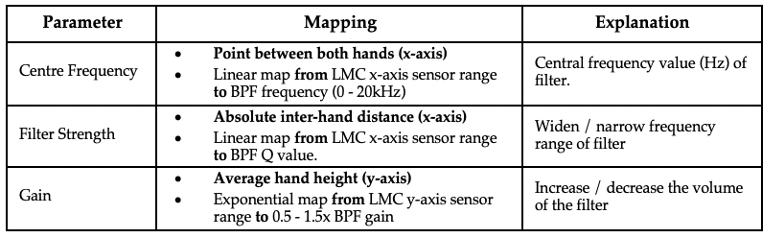
\includegraphics[width=0.8\linewidth]{figures/05-area/areatechnical_param1.png}
    \caption{Band-pass filter parameter mappings}
    \label{fig: areaparams1}
\end{figure}

\begin{figure}
    \centering
    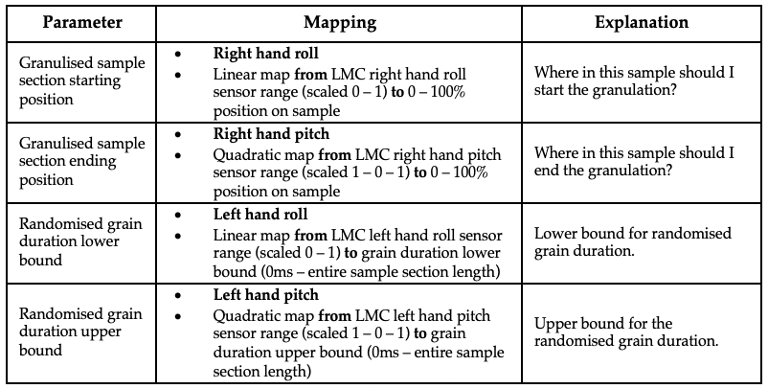
\includegraphics[width=0.8\linewidth]{figures/05-area/areatechnical_param2.png}
    \caption{Granular synthesiser parameter mappings}
    \label{fig: areaparams2}
\end{figure}
When the composer decides to end manipulating the sample, they can do so by performing a grab with both hands. Once this happens, the band-pass filter and granular synthesis parameters are frozen for that sample.

\subsubsection{Spatialise}                      \label{sec: area-system-software-spatialise}
\textbf{The spatialise stage} begins once the manipulation stage has ended. The three-dimensional space above the LMC is mapped to the \textit{virtual audio environment}, in which the composer is currently listening to the sample that they have recorded. The composer can use their right hand to move the sample around the \textit{virtual audio environment}. For an example of the effect this has, moving the hand between the two extremes of the x-axis (left to right) results in hearing the sample move from ear to ear. The spatialise stage is ended by grabbing with the right hand.

Once the spatialise stage has ended, the composer has the option to repeat the process 7 more times, allowing for the creation of a \textit{virtual audio environment} comprised of up to 8 spatialised audio samples, or what I refer to as \textit{nodes}. 

\subsubsection{Summary}                         \label{sec: area-system-software-summary}
The audio signal arriving in the two conduction pads in the headphones are the signals of two equidistantly spaced virtual microphones inside the \textit{B-Format virtual audio environment} that decode it into two channels, left and right. Further interaction comes from composer head movement which, at all times, is mapped to the revolution of these two virtual microphones around the central point of the \textit{virtual audio environment}. This means if there is a node playing to the left of the composer, rotating the head 90° anticlockwise results in the \textit{node} now sounding as if it is in front of the composer’s face. This is achieved via the ICST Ambisonics Library \citep{schacher2006} \footnote{\url{https://www.zhdk.ch/forschung/icst/software-downloads-5379/downloads-ambisonics-externals-for-maxmsp-5381}}and is elaborated on in the sections \autoref{sec: area-study-results-experiences} and \autoref{sec: area-discussion-aar}, but for now it is worth mentioning that it allows for immersion into a combined \textit{real and virtual audio environment}.

To summarise, the patch can be categorised into having two inputs: audio from the composer’s environment and hand gesture, and one output: \textit{the virtual audio environment}. In the background, this audio input is decoded into the \textit{ambisonic palette} (inaudible), which is acted on by the composer’s hands to form one audible output: the \textit{virtual audio environment}, which is comprised of up to 8 \textit{nodes}. Through the choice of sensory overlay (bone conduction) and integration of head tracking, this \textit{virtual audio environment} is experienced synchronously with the composers’ real, multisensory environment. 



% --------------------------------------------------------------------------- %
\section{Composing with \textit{area\textasciitilde{}}} \label{sec: area-study}
\subsection{Autobiographical Design}            \label{sec: area-study-abd}
Originally, the study was planned for late March and would involve several participatory interaction studies. However, due to the UK lockdown in response to the unfolding COVID-19 pandemic, this was postponed until later in the year. Instead, I investigated the system using an autobiographical design method, framing it as a hypothesis study to better understand relationships between virtual and real environments, in the hope of developing a practice-led method for creating and researching multisensory augmented reality experiences. 

Autobiographical design is defined as “design research drawing on extensive, genuine usage by those creating or building the system” \citep{neustaedter2012}. Neustaedter and Sengers define “genuine usage” here to mean that changes are “based on the true needs of the researchers, rather than them pretending to have needs expected of target users”.

Due to the lockdown, and therefore inability to conduct in-person user-tests, this research method was beneficial as I was spending large amounts of time with the system. Moreover, there are several suggested requirements of employing this research method that Neustaedter and Sengers highlight that are true of the \textit{area\textasciitilde{}} system:
\begin{itemize}
    \item The existence of a genuine usage of the system
    \item The system being already developed
    \item The ability for fast tinkering 
    \item Record-keeping of the design process
    \item Long-term usage of the system
\end{itemize}
Furthermore, as AR technology moves towards being a component of future general personal computing, there is a need for first-person research methods that take into consideration the effects of prolonged system usage as well as the arising relationship between participant and system \citep{desjardins2018}. Moreover, these methods have been found to be specifically relevant to wearable systems \citep{cecchinato2017}.

A disadvantage of using autobiographical design as a research method is its inability to establish generalisability (also the case with ethnography, case studies and participatory workshops), which is why I opted for participant studies in the evaluation of \textit{polaris\textasciitilde{}} in \autoref{sec: polaris}.

\subsection{Design} \label{sec: area-study-design}
The study was designed as a cycle, in order to promote fast tinkering, record-keeping, and long-term usage in line with autobiographical design guidelines. 
\begin{enumerate}
    \item Over three sessions, ideally during the same week, the system is used with a logbook at hand in order to facilitate record-keeping of hardware setup, \textit{node} manipulation and completed \textit{real and virtual audio environment} listening experience remarks.
    \item After each session, the notes are formalised into a database and categorised as "composer experience remarks” or “improvement remarks”.
    \item At the end of the week, the three sessions’ notes are summarised into a “check-in” document, where composer experience remarks are collated, and improvement remarks are further categorised into lists pertaining to the area of the system that needs improvement or change.
    \item Those changes are then made to the system and the cycle restarts.
\end{enumerate}

\subsection{Results}                            \label{sec: area-study-results}
\subsubsection{Hardware Location}               \label{sec: area-study-results-hwloc}
I have observed that an environment with a lower noise floor is desirable and have implemented a normaliser to deal with re-recording loud background / ambient noises during successive \textit{node} recording. I found myself basing the choice of microphone placement on what I wanted the \textit{virtual audio environment} to sound like. Since the system uses an ambisonic microphone, consideration of the spherical 360° field of the microphone would lead to a richer \textit{ambisonic palette} and subsequent \textit{virtual audio environment}.

Two sessions were based outdoors and involved natural sounds such as birds, trees and wind, as well as passing cars. One of the sessions was inside and took place at the same time my partner was on a Zoom call, and therefore the \textit{ambisonic palette} was invariably based on her speech and my movement and action inside the room. I want to look into placing the microphone inside bushes, trees, etc. rather than in open spaces to explore aesthetically the \textit{virtual audio environment} that arises from such placement. Furthermore, the relationship between \textit{real and virtual audio environment} would be quite different. Through their ears, the composer would be rooted in their position in the environment, but because of the inherent blend between hearing and bone conduction, they would simultaneously experience the sonic environment of the bush mediated by the Max MSP patch.

\subsubsection{Experiences}                     \label{sec: area-study-results-experiences}
The system takes considerable time to set up, especially when documenting with video, audio, and notes. This process could certainly be streamlined further. Overall, I was pleased with the sound quality; the microphone picks up the environment very clearly. However, I remarked that the manipulation stage could feature more interesting real-time auditory effects on the \textit{nodes}. The blending of \textit{real and virtual audio environment} is achieved well via the bone conduction headphones and there was a subconscious registration via the head-tracking that gave me the very real impression that there was a 3D environment of \textit{nodes} around my body.

The IMU on the bone conduction headphones sometimes provides erratic and erroneous data, leading to accidental revolutions of the \textit{virtual audio environment} around the head. Despite technical difficulties such as this, in one autobiographical design session, when I took the headphones off, I wrote that “I felt like I'd been disconnected from something” and that “my senses felt heightened before I took them off, not only to the \textit{virtual audio environment}, but now more sensitive to the audio content of my real environment.

If I managed to capture an infrequent environment sound, such as a particular bird call, or a sentence of spoken word, the fact that the patch is set up to loop the samples gave a certain permanence to that otherwise impermanent sound. On multiple occasions I could not tell if the sounds of birds I was hearing originated from a \textit{node} or from within a tree.

\subsubsection{Arising Interactions}            \label{sec: area-study-results-arisingints}
The maximum sample length is currently 28 seconds, but I have found myself mainly sticking to shorter loops, creating quite repetitive and rhythmic sequences. I remarked that grains from the synthesiser sounded like a permanent record of my gestures’ effect on the environment. I liked the playfulness of being able to record a sound from a certain location in my \textit{real audio environment} and place it in different location in my \textit{virtual audio environment}.

Despite the wearable hardware being wireless, hand interaction with the \textit{area\textasciitilde{}} system is inherently limited to being in range of the LMC (often placed on a table). I found myself wanting to be able to move around my environment whilst being able to record new nodes and hear existing nodes move relative to my body position.
\section{Evaluating \textit{area\textasciitilde{}}} \label{sec: area-discussion-aar}
Overall, the results from my autobiographical design method have shown that \textit{area\textasciitilde{}} is an effective tool for examining the combinatorial relationship between real and virtual environments. Despite the system’s hardware setup requiring some further work to allow for quicker start up and more accurate head tracking, it has provided me with novel aesthetic experience through:
\begin{itemize}
    \item The blending of \textit{real and virtual auditory environments} to create a third, augmented environment that was greater in experiential nature than the sum of its parts (not simply a combinatorial layering)
    \item The ability to spectromorphologically manipulate sounds in real-time in this third environment with the body
    \item The potential for creating believable illusions of real-world sound sources from these manipulated and spatialised virtual sounds.
\end{itemize}

The tables of parameter mappings shown in \autoref{sec: area-system-software-manip} may seem like a chaotic mess, however, time has been spent making these mappings intuitive. For example, the representation of volume to a vertical scale corresponds with findings that non-musicians are relatively competent at attributing the size of air-gestures to heightened musical dynamics \citep{godoy2006,caramiaux2010}. As for the band-pass filter’s horizontal pitch mappings, this is mainly based on the visual representation of frequencies on a horizontal scale often found in the user interface of such filters. Nevertheless, it is pertinent to mention that field of psycho-musicology research \citep{timmers2016} finds a correlation between pitch representation and horizontal space i.e. lower pitch to the left, higher pitch to the right. Although this is often attributed to the internalised representation of horizontal pitch on pianos by keyboard-playing musicians \citep{lidji2007,rusconi2006}, it has been found that this effect also propagates in non-musicians \citep{weis2016}. This is also found to be the case in the “Playing air-instruments” study carried out by Godøy, Haga, and Jensenius \citeyearpar{godoy2006}.

In contrast, interaction with the granular synthesiser is not made to be intuitive; instead, I have opted to hide or black-box the interaction through a mix of linear and quadratic mappings on each hand. This is in order to stir curiosity in the composer and induce play, as I found in \autoref{sec: area-study-results-arisingints}: “I remarked that grains from the synthesiser sounded like a record of my gestures’ effect on the environment”.

Indeed, whilst outlining the material epistemologies of digital music instruments (DMIs), \citep{magnusson2009} describes black-boxed DMIs as containing  “knowledge of its inventors, which means that the users of the instrument do not need to have a deep knowledge of its internal functions”, furthermore clarifying that there is a “continued oscillation between a mode of conceptual (system design) engagement with the instrument and [an] embodied (performative) relationship with it”. This ‘oscillation’ displays, in turn, an underlying synergy between DMI development and the autobiographical design process, perhaps due to the similarities in requirements of the processes outlined in \autoref{sec: area-study-abd}. This synergy has led to the use of ABD in the development of many DMIs and interactive music systems \citep{kiefer2020,martin2017,turchet2018,unander-scharin2014}.

\begin{figure}
    \centering
    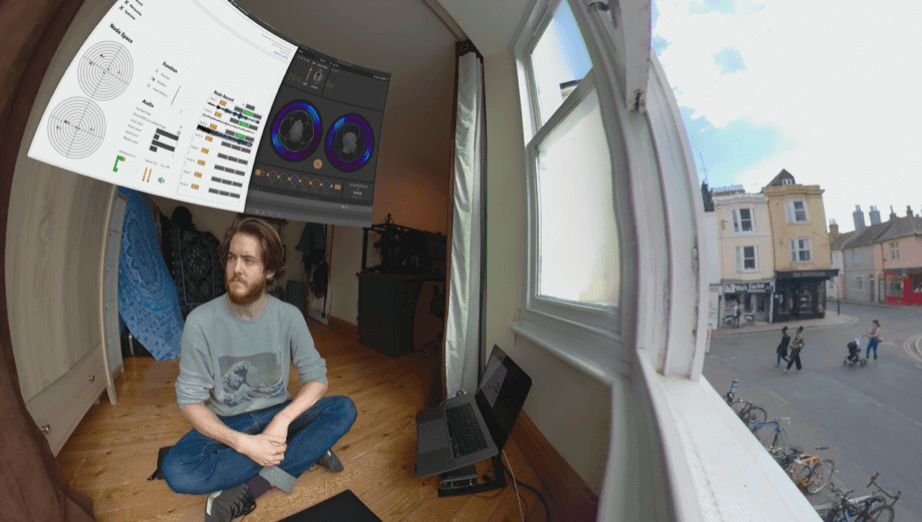
\includegraphics{figures/05-area/areafuturedoc.png}
    \caption{\textit{area\textasciitilde{}} 360° video and ambisonic documentation \rurl{youtu.be/SPd-f2EXuIQ}}
    \label{fig: areafuturedoc}
\end{figure}
As a system for creating computational sound ARt in the form of in-situ AAR experiences, \textit{area\textasciitilde{}}’s artistic output is firstly a real-time compositional experience. In order to document these experiences of the system however, I have included the automated recording and saving of both the \textit{ambisonic palette} (the ambisonic recording of the real audio environment), and the users \textit{virtual audio environment} as separate B-Format .wav files in the project directory. These separate B-Format .wav files could be merged and decoded from B-Format to any number of speakers for a multi-channel installation of field recordings or manipulations of environments made with \textit{area\textasciitilde{}}. This also leaves open the potential for \textit{area\textasciitilde{}} to be used as a compositional tool for interactive soundscape composition.

I also chose to merge and decode a set of these recordings to binaural stereo format, and have time-synced this recording with a 360° video and a screen recording of the patch that was taken during the system’s use. This allows my composition of the \textit{virtual audio environment} to be experienced second-hand with headphones. Dragging the screen in different directions with mouse/touchscreen emulates hearing the difference in environment if I moved my head in those directions. Optionally, an inexpensive smartphone VR headset (£5 - £15) can be used to heighten the interactivity of the experience. A screenshot of the 360° video \citep{bilbow2020} is shown in \autoref{fig: areafuturedoc}. The potential for users’ experiments with \textit{area\textasciitilde{}} to be captured and re-experienced interactively could have interesting applications, effectively allowing users to explore each others’ lived aural experience of the system.
% --------------------------------------------------------------------------- %



%The  novel experiences that emerged from the results of the study into the uses of AR as a medium for computational art have encouraged me to devise a practice-led method for researching multisensory AR (MSAR). It begins with the ideation of an MSAR Experience (which describes a possible human-to-sense interaction). These are classed as Snippets, Scenes, and Spaces depending on the number of senses engaged, sensory intensity, and interaction size. The hardware and software that enable the experience are classed as MSAR Instruments and MSAR Environments respectively. Instruments are categorised into Wearable, Tangible and Situated Instruments. This taxonomy will eventually aid not only in the creation, but in the evaluation of future MSAR Experiences. 
  \clearpage% --------------------------------------------------------------------------- %
%                  _             _   _                                        %
%   _____   ____ _| |_   _  __ _| |_(_)_ __   __ _                            %
%  / _ \ \ / / _` | | | | |/ _` | __| | '_ \ / _` |                           %
% |  __/\ V / (_| | | |_| | (_| | |_| | | | | (_| |                           %
%  \___| \_/ \__,_|_|\__,_|\__,_|\__|_|_| |_|\__, |                           %
%                                            |___/                            %
%                                                    _            _           %
%                                        _ __   ___ | | __ _ _ __(_)___       %
%                                       | '_ \ / _ \| |/ _` | '__| / __| /\/| %
%                                       | |_) | (_) | | (_| | |  | \__ \|/\/  %
%                                       | .__/ \___/|_|\__,_|_|  |_|___/      %
%                                       |_|                                   %
% --------------------------------------------------------------------------- %
\chapter{Evaluating polaris\textasciitilde{}}\label{sec: polaris}
\begin{flushright}
    \Large\textsc{An Audiovisual Augmented Reality Experience Build on Open-Source Hardware and Software}
\end{flushright}
%\markboth{}{Evaluating polaris\textasciitilde{} - An Audiovisual Augmented Reality Experience Build on Open-Source Hardware and Software}
\begin{SingleSpace}
    \noindent\textbf{polaris\textasciitilde{} Blog: } \url{https://www.sambilbow.com/projects/polaris}
    
    \noindent\textbf{polaris\textasciitilde{} Code: } \url{https://www.github.com/sambilbow/polaris}
    
    \noindent\textbf{polaris\textasciitilde{} Guide: } \url{https://www.github.com/sambilbow/polaris/wiki}
    
    \noindent\textbf{polaris\textasciitilde{} Publication: } \url{https://dx.doi.org/10.21428/92fbeb44.8abb9ce6}
\end{SingleSpace}

\begin{figure}
    \centering
    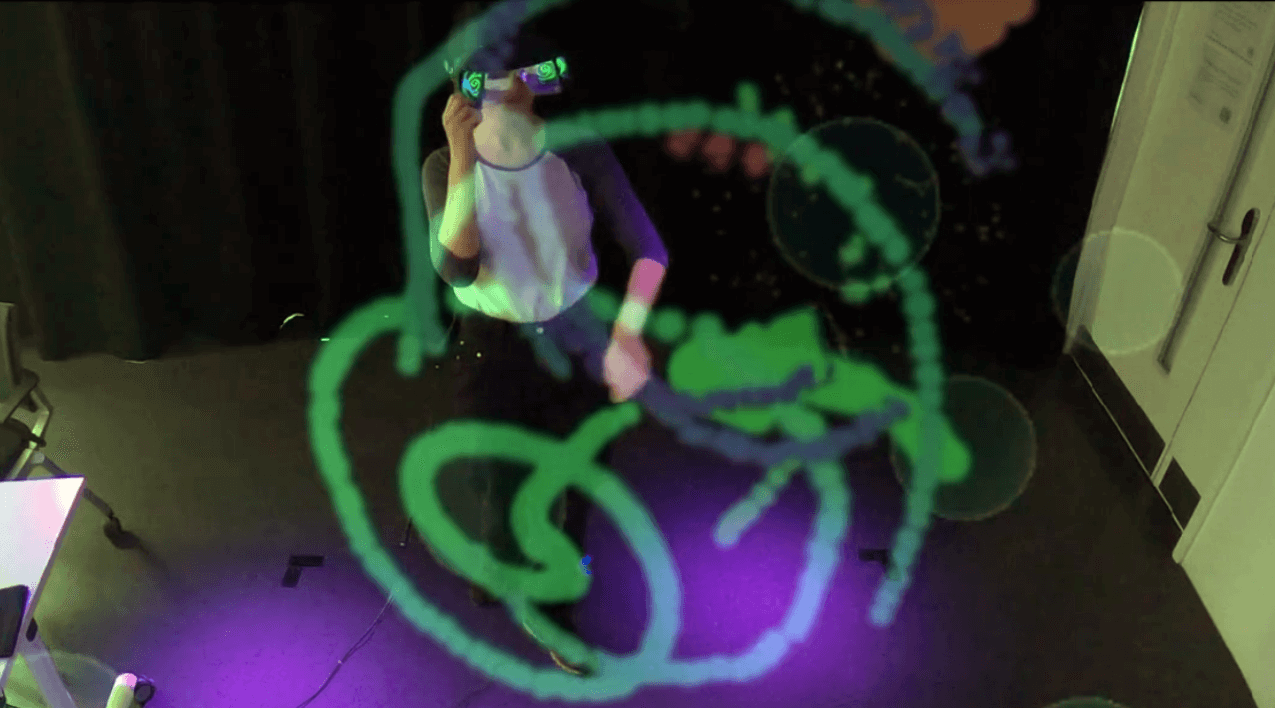
\includegraphics[width=1\linewidth]{06-polaris/chapter-fig.png}
    \captionsetup{labelformat=empty}
    \caption[\autoref{sec: polaris}: Experience Study of \textit{polaris\textasciitilde{}} at the Sussex Humanities Lab, (from \citeauthor{bilbow2022}, \citeyear{bilbow2022})]{}
\end{figure}

    
\clearpage
   
% --------------------------------------------------------------------------- %
\section{Summary}\label{sec: polaris-summary}
This chapter outlines the development and evaluation of the \textit{polaris\textasciitilde{}} experience. \textit{polaris\textasciitilde{}} is built using a set of open-source hardware and software components that can be used to create privacy-respecting and cost-effective audiovisual AR experiences. Its wearable component is comprised of the open-source Project North Star AR headset and a pair of bone conduction headphones, providing simultaneous real and virtual visual and auditory elements. These elements are spatially aligned using Unity and PureData to the real space that they appear in and can be gesturally interacted with in a way that fosters artistic and musical expression. In order to evaluate the \textit{polaris\textasciitilde{}}, 10 participants were recruited, who spent approximately 30 minutes each in the AR scene and were interviewed about their experience. Using grounded theory, the author extracted coded remarks from the transcriptions of these studies, that were then sorted into the categories of Sentiment, Learning, Adoption, Expression, and Immersion. In evaluating \textit{polaris\textasciitilde{}} it was found that the experience engaged participants fruitfully, with many noting their ability to express themselves audiovisually in creative ways.

The objective of this chapter is to evaluate \textit{polaris\textasciitilde{}} as an AR experience for its ability to provide a space for gestural audiovisual expression, primarily through a user study, and later using the grounded theory method to extract relevant themes from participant interactions. The outcome of this research has contributed thoroughly to the design patterns in \autoref{sec: discussion-patterns}.



% --------------------------------------------------------------------------- %
\section{Designing \textit{polaris\textasciitilde{}}}\label{sec: polaris-framework}
The \textit{polaris\textasciitilde{}} experience itself is built using mostly open-source hardware and software. As well as creating the experience, I was interested in keeping a log of its framework in order to ensure its reproducibility and to facilitate further creation of a wide variety of audiovisual AR experiences. Any `artist-developer' \footnote{By using the term artist-developer, I refer to the media artist, creative coder, digital musician, or indeed any of the other many terms used to describe the category of artist who uses code and/or technology as their medium of artistic expression.} wanting to work on similar experiences should have the ability, when following this framework, to rapidly create and prototype low-cost and privacy-respecting sound ARt experiences, and instruments..

\subsection{\textit{polaris\textasciitilde{}} Hardware}\label{sec: polaris-framework-hardware}
\subsubsection{Project North Star}\label{sec: polaris-framework-hardware-pns}

\begin{figure}
    \centering
    \subcaptionbox{Playing a virtual piano\label{fig: polaris-framework-hardware-pns-1}}{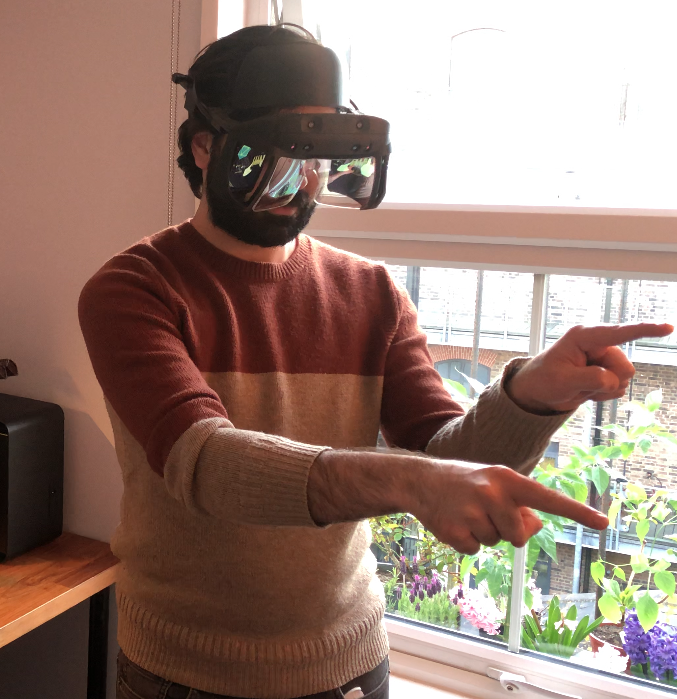
\includegraphics[height=3.5cm]{figures/06-polaris/polaris-framework-hardware-pns-1.png}}
    \hspace*{0.75cm}
    \subcaptionbox{Resizing and moving virtual objects\label{fig: polaris-framework-hardware-pns-2}}{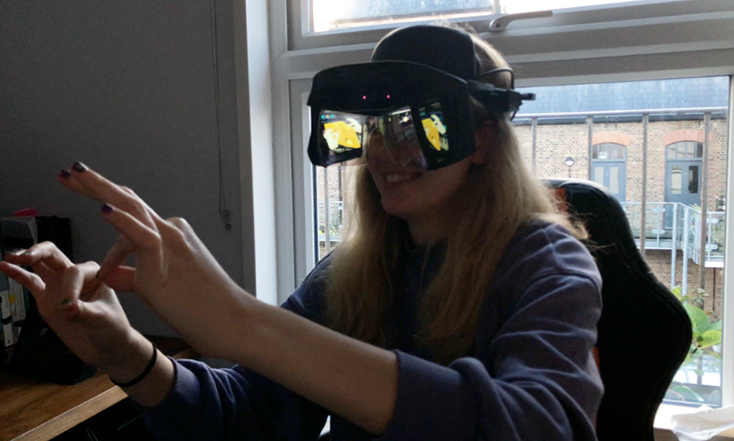
\includegraphics[height=3.5cm]{figures/06-polaris/polaris-framework-hardware-pns-2.png}}
    \caption{Project North Star in use}
\end{figure}

The primary section of wearable hardware is the Project North Star (NS) AR headset, as open-sourced by LeapMotion (now Ultraleap) in 2018. It has a 3D-printable assembly, and its circuit boards, cables, and screens are available to buy \href{https://docs.projectnorthstar.org}{online}; my North Star cost about £500 in total to build - 5 to 6 times less expensive than the commercial AR headsets mentioned, while maintaining industry-leading hand-tracking and 6DoF (6 degrees of freedom) depth tracking.

However, the time needed to build one and understand its workings well enough to trouble\-shoot any issues one faces may be a barrier to entry \footnote{I have found it a surprisingly integral part of the way I make sense of my creative practice, and fortunately there is a Project North Star Discord server with over 2400 helpful members that I have relied on heavily!}. Additionally, the finish material is not as polished as commercial headsets, and the overall size is larger and clunkier. It also needs to be tethered by USB and DisplayPort cable to a host computer or mobile compute pack.

Despite these drawbacks, my own experience of the headset has led to the rapid creation of many audiovisual AR prototypes. The fact that it requires no account to use, no developer's license to work with, and no data to be sent away to corporate servers has only added to my comfortability of using it as a creative tool.

\begin{wrapfigure}{r}{0.45\textwidth}
    \vspace{-\intextsep}
    \hfill
    \begin{minipage}{0.95\linewidth}
            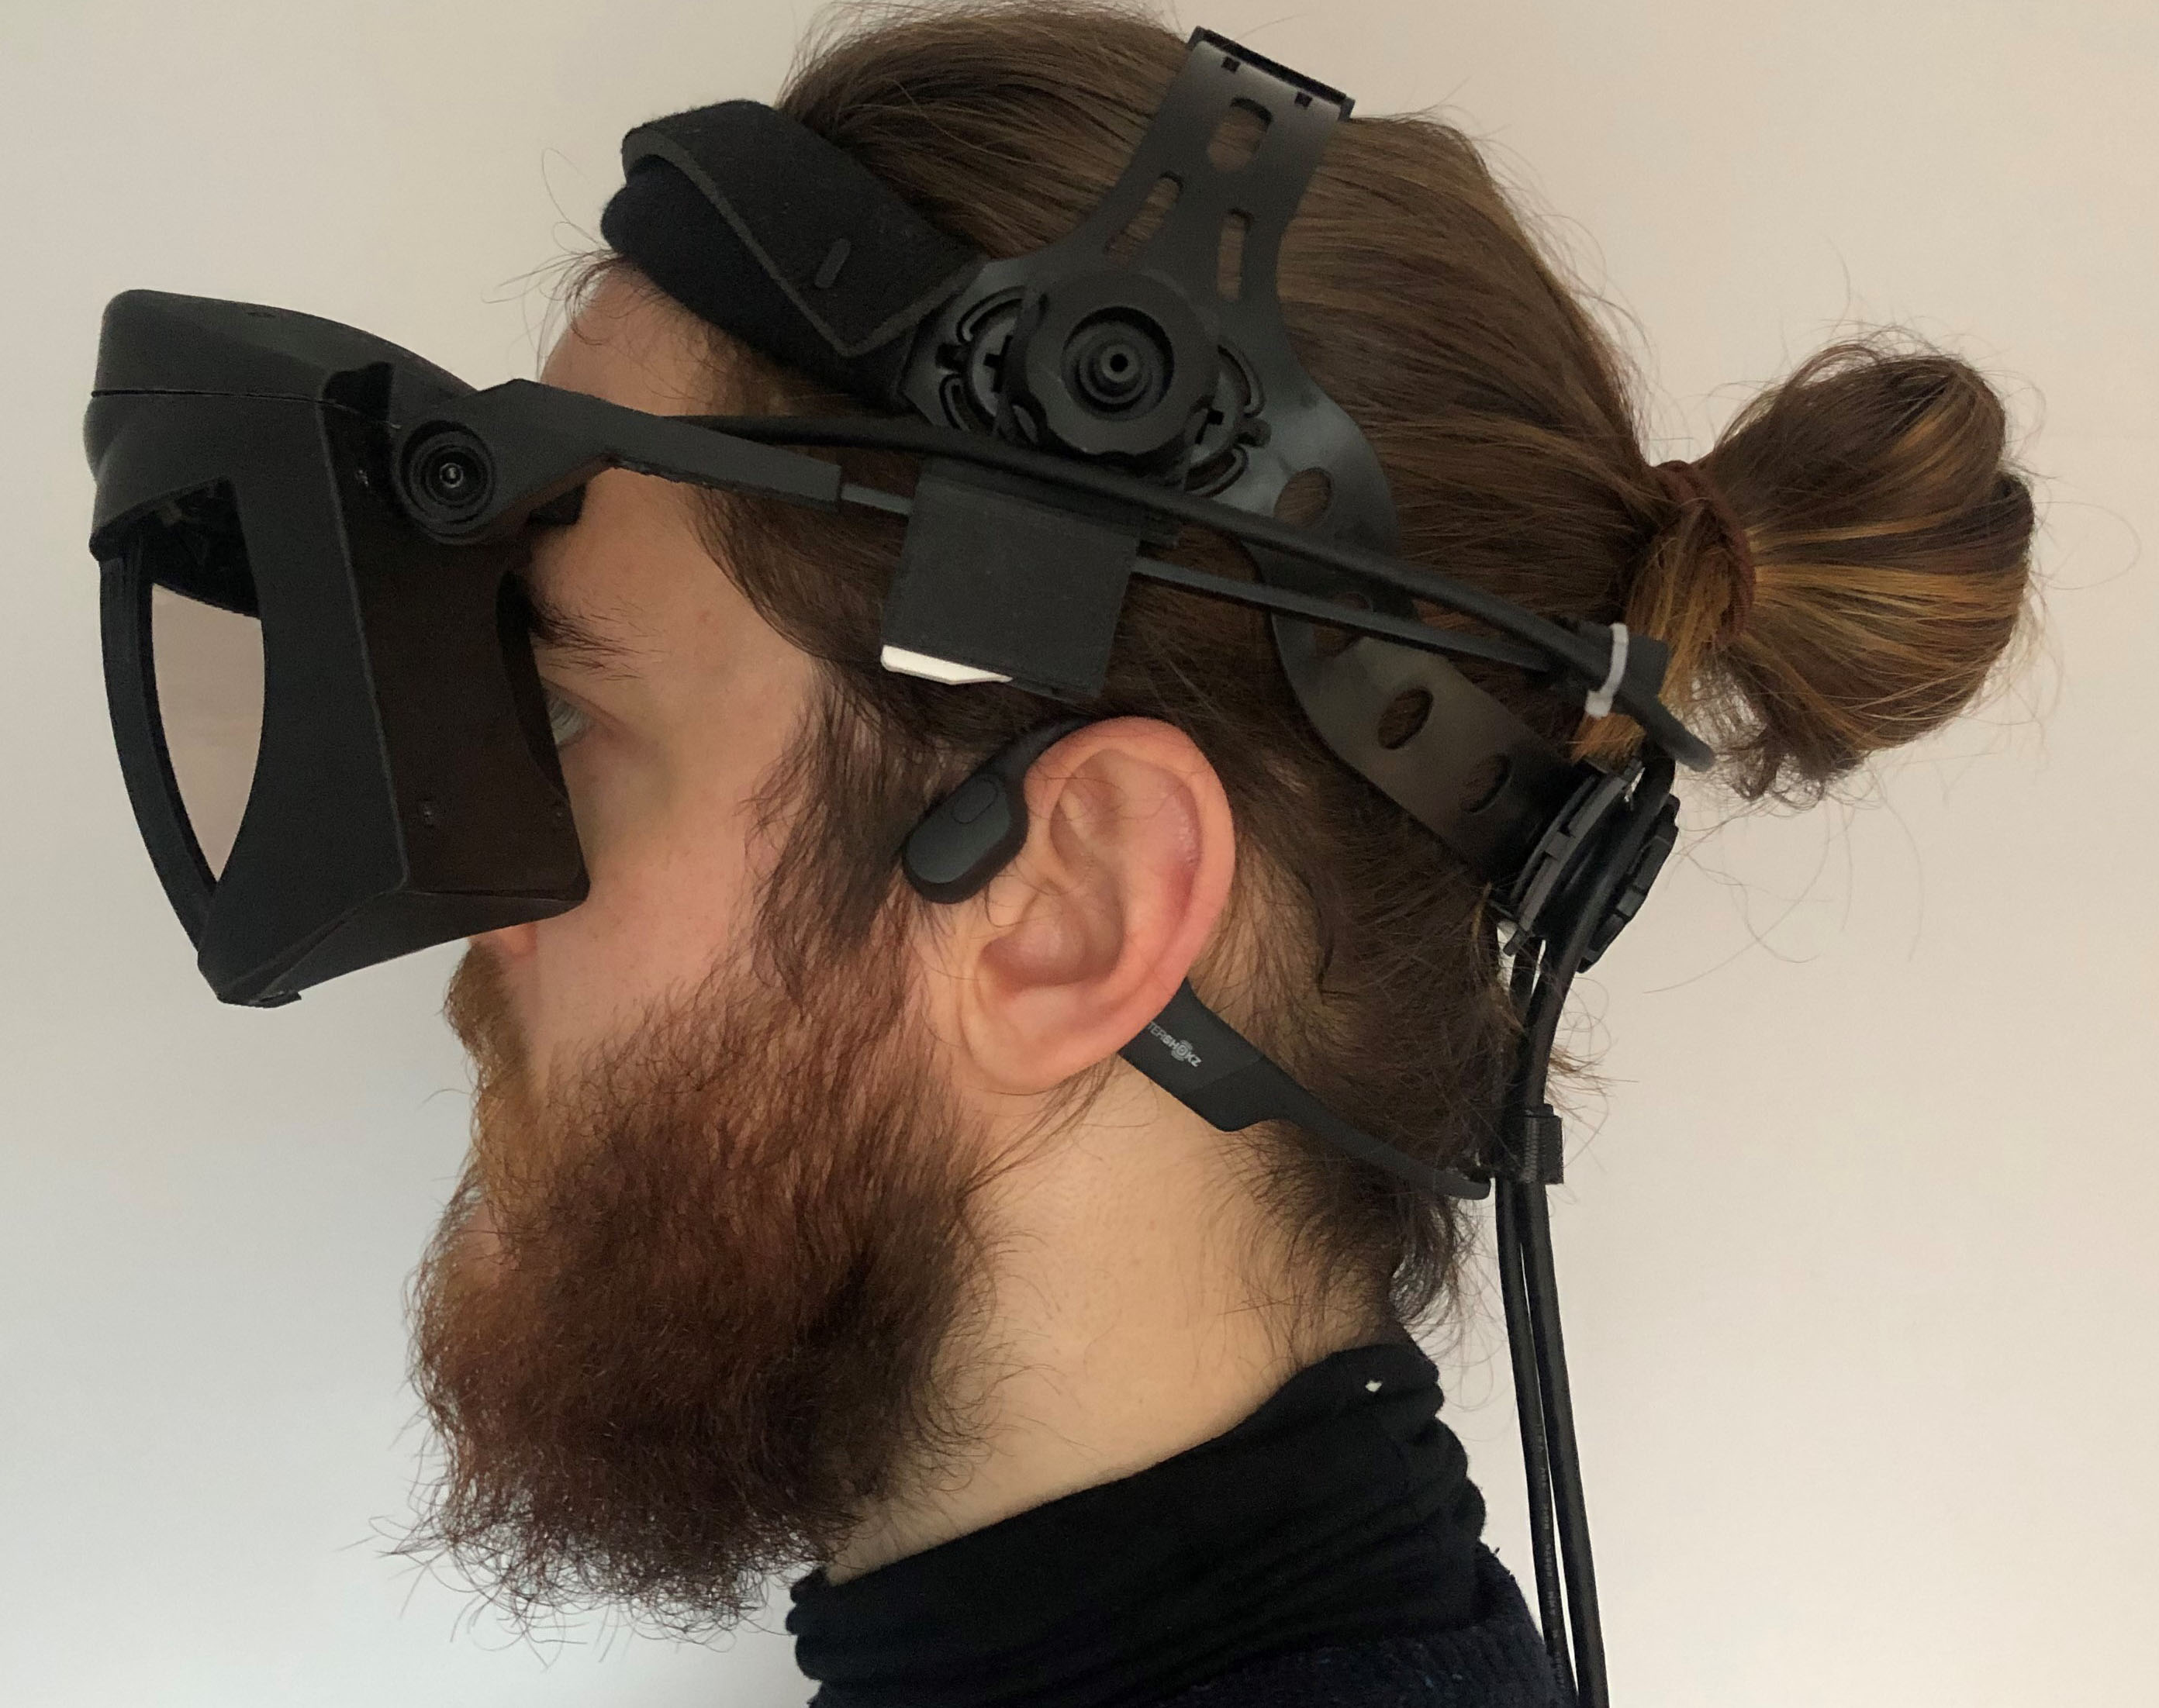
\includegraphics[width=\linewidth]{figures/06-polaris/polaris-framework-hardware-bc.jpg}
            \captionsetup{justification=justified}
            \caption{Project North Star worn with the addition of bone-conduction headphones}\label{fig: polaris-framework-hardware-bc}
    \end{minipage}
\end{wrapfigure}
\subsubsection{Bone Conduction}\label{sec: polaris-framework-hardware-bc}
The secondary piece of hardware in the system is a pair of bone-conduction headphones, seen in \autoref{fig: polaris-framework-hardware-bc}. These have been used as a method of auditory display in several other AR projects \citep{lindeman2008,barde2016,chevalier2018}, typically for their ability to deliver audio in an unobtrusive fashion, as well as their comfortability and cleanliness in installation settings. They do not obscure the wearer's hearing of their real environment, making them suitable for emphasising the intertwined nature of virtual and real components of an AR experience.


\subsection{\textit{polaris\textasciitilde{}} Software}\label{sec: polaris-framework-software}
\subsubsection{Unity}\label{sec: polaris-framework-software-unity}
\textit{polaris\textasciitilde{}} uses an open-source software companion to the NS headset developed and maintained by Damien Rompapas \citeyearpar{rompapas2020}. At run-time, this Unity plugin (also making use of Ultraleap's Hands plugin) computes sensor readings from both the hand- and movement-tracking sensors and recreates the hand and headset pose in real-time inside the Unity scene. With the pose computed, it outputs the resultant view to the displays of the headset, rendering anything in the Unity scene relative to it.

Thanks to Unity's in-built audio spatialisation, any audio sample attached to an object in the Unity scene is, by default, spatialised in 3D and output via the bone-conduction headphones.

\subsubsection{PureData}\label{sec: polaris-framework-software-puredata}
In my own research, the desire to implement more than just sample-based audio interactions led me to experiment with many different options for implementing real-time audio synthesis. I ranked each option I found by its ability to fulfil the below criteria: (a write-up can be found on \href{https://sambilbow.github.io/projects/polaris/software.html}{my website})

\begin{enumerate}
    \item Uses Unity's in-built audio spatialisation.
    \item Low computational cost on the host computer, and ability to be instantiated tens to hundreds of times procedurally.
    \item Ability to afford the artist-developer a wide palette of synthesis techniques.
    \item Allowing real-time parameter control of sounds via movement, gesture, and interaction with GameObjects in the Unity scene.
    \item Ability to rapidly prototype sound synthesis techniques and sonic interactions.
    \item Being free, open-source, and cross-platform.
\end{enumerate}

Meeting all these requirements was the \href{https://github.com/LibPdIntegration/LibPdIntegration}{LibPdIntegration} project developed and maintained by Niall Moody and Yann Seznec. It allows for the use of PureData patches in Unity, which, at run-time, are compiled to libPd (an embeddable version of PureData), and whose output is fed in real-time to the sound output of the GameObjects they are attached to  \footnote{The inclusion of PureData means that the many artist-developers can rely on a program that has existed in the field for nearly 25 years, many of whom will have experience using it.}.

To summarise, the use of the North Star companion software in conjunction with LibPdIntegration, allows for the creation of objects in an AR scene that can have their own PureData patches. These can be parametrised to gesture, movement, and interaction, in ways that manipulate their audio synthesis in real-time and at low computational cost. This all while existing three-dimensionally in the participants' visual and auditory fields. The fact that this is delivered via an optical-see through headset and bone-conduction headphones results in an experience that does not significantly hinder (compared to VR) the participants' ability to see and hear their real environment - augmenting and hybridising reality rather than replacing it.



% --------------------------------------------------------------------------- %
\section{Participant Studies}\label{sec: polaris-study}
In 2021, I ran a participant experience study of \textit{polaris\textasciitilde{}}, the first experience I created with the above framework. The main objective of the study was to extract (via grounded theory) participant sentiment towards their ability to audiovisually express themselves through gesture and movement in the AR experience. Participants were recruited via university mailing-list, and were a mix of undergraduate and postgraduate Media, Film, and Music students.

\subsection{Questionnaire}\label{sec: polaris-study-questionnaire}
Participants completed a questionnaire, in which I asked for their age, gender identity, ethnicity, and occupation, to ensure a diverse and inclusive variety of participants. The mean age was \textasciitilde{}24.7 years old, with a range between 19 and 37; there were 6 female and 4 male participants, belonging to a diverse group of ethnicities.

\subsection{Tutorial}\label{sec: polaris-study-tutorial}
The participants were inducted into the experience via an introductory five-minute tutorial, the purpose being to ensure safety, build trust, and allow space for questions before beginning. This took the form of a narrated slideshow, in which I outlined the devices and interactions they should expect in the experience.

\subsection{The \textit{polaris\textasciitilde{}} Experience}\label{sec: polaris-study-experience}
Once the participant was wearing the headset and headphones, confirmed they were comfortable and they were standing in the starting position \footnote{As the headset was tethered to a computer, keeping the starting position the same between participants meant that the position of virtual content could be approximated to a clear space in the lab, marked by tape on the floor}, I began the Unity scene (a full demonstration of the scene can be found on my \href{https://youtu.be/lCBgMs8ULj0}{YouTube channel}), and let them know that the experience was about to start.

The experience involved nine floating iridescent `orbs', scattered at different distances from the starting position. The orbs would individually emit a repeating tone, whose pitch and tempo varied from orb to orb. Upon emitting a sound, the orb would eject a shower of white particles.

[iframe element]

Participants were invited to explore the space at their own pace. They could, of course, view the orbs from different angles, and hear their tones get louder and quieter as well as panning from ear to ear as they walked around them.
I then prompted them to direct their gaze towards their hands, which were outlined, and when turning the left hand to face them, a menu appeared to the right of their palm. The menu contained two buttons, one labelled `Change Hand Colour', the other `Toggle Interactions'. I prompted them to tap the top button, which upon depressing slightly and providing an auditory `click', changed the colour of their hand's outline.

[iframe element]

Upon toggling the second button on, constant streams of particles started emitting from the centre of their palms. These particles persisted for approximately five seconds to conserve computational power. While the button was toggled on, and the streams were emitting, each hand also produced a continuous noise.

In addition to these interactions, a total of five further interactions existed in the experience. The first two concerned the position, orientation, and gesture of the hands, relative to the participant. Firstly, they could modulate the depth of a vibrato effect on the sound of the particle stream by gradually turning their palms towards their face. Secondly, they could affect the sound's filter cut-off frequency by pinching their fingers together into a point, resulting in a hissing sound; paired with the visual feedback of narrowing the particle stream.

[iframe element]

On pointing their palms in the direction of an orb, the particles would gravitate towards the orb, and begin to slow down, orbit, and rotate it. Depending on which palm was pointing towards the orb, there would be an additional effect that increased in intensity as the participant persisted in pointing towards the orb. When pointing their left palm, over the course of 20 seconds, the orb's tone and white particle burst increased in tempo. When pointing their right palm towards an orb, over the course of 5 seconds, the depth of a tremolo effect on that orb's tone increased, with the paths of the white particles emitted from the orb becoming more erratic and corkscrew-like.

[iframe element]

Exploration of the scene differed between participants, but once they had either found or been shown the interaction methods in the scene and had either explored their variety or asked if there was anything else that they could do, I would ask them to try some experimental interactions.

Taking advantage of the vast number of parameters available to edit in Unity, I then changed elements of the visual   experience \footnote{Since the 11 PureData patches (9 for the orbs, and 1 each for the hands) were compiled at run-time they could not be edited on the fly} in real-time, asking for participant feedback on elements they preferred, and why. These elements of visual experience involved the orbs size, shape, gravity strength, and range; particle size, speed, lifetime, and colour.

[iframe element]

\subsection{Interview}\label{sec: polaris-study-interview}
The next step of the study was a 10-minute interview, in which I asked participants about the positive and negative aspects of the experience, and anything they could suggest that would improve the experience. Questions were left deliberately broad due to the use of grounded theory to draw out themes for later analysis. I used a topic guide (see Appendix 1) to keep follow-on questions for replies related to the experience. This was in the form of a set of questions from the validated questionnaire titled `User Experience in Immersive Virtual Environments' by Katy Tcha-Tokey et al. \citeyearpar{tcha-tokey2016a}, which I adapted to suit AR.

% --------------------------------------------------------------------------- %
\section{Results}\label{sec: polaris-feedback}
\subsection{Grounded Theory}\label{sec: polaris-feedback-grounded}
I chose the constructivist strand of grounded theory as developed by Kathy Charmaz \citeyearpar{charmaz2006} (building on the initial work by Glaser and Strauss \citeyearpar{glaser1967}) for my method of data analysis due to its ability to build theories from gathered data. Generally, generating a grounded theory extracts relevance from `codes' - line-by-line summaries of transcribed speech, that are then iteratively and repeatedly refined, and sorted into categories. This contrasts approaching data collection with a specific hypothesis in mind.

In the constructivist version of the Grounded Theory method, rather than assuming emergence of `unproblematic' and `objective' categories from the data itself, categories are admitted to being `mutually constructed' through interaction by the researcher with the data, considering and highlighting both the position and subjectivity of the researcher, as well as the partiality, and situational nature of the data itself.

In this instance, a study where I set out to evaluate the experience of participants in an audiovisual AR scene, I believed that it was suited to provide a rich set of data from which to critique and iterate the experience, and eventually build a set of multisensory AR design guidelines.

\begin{figure}
    \centering
    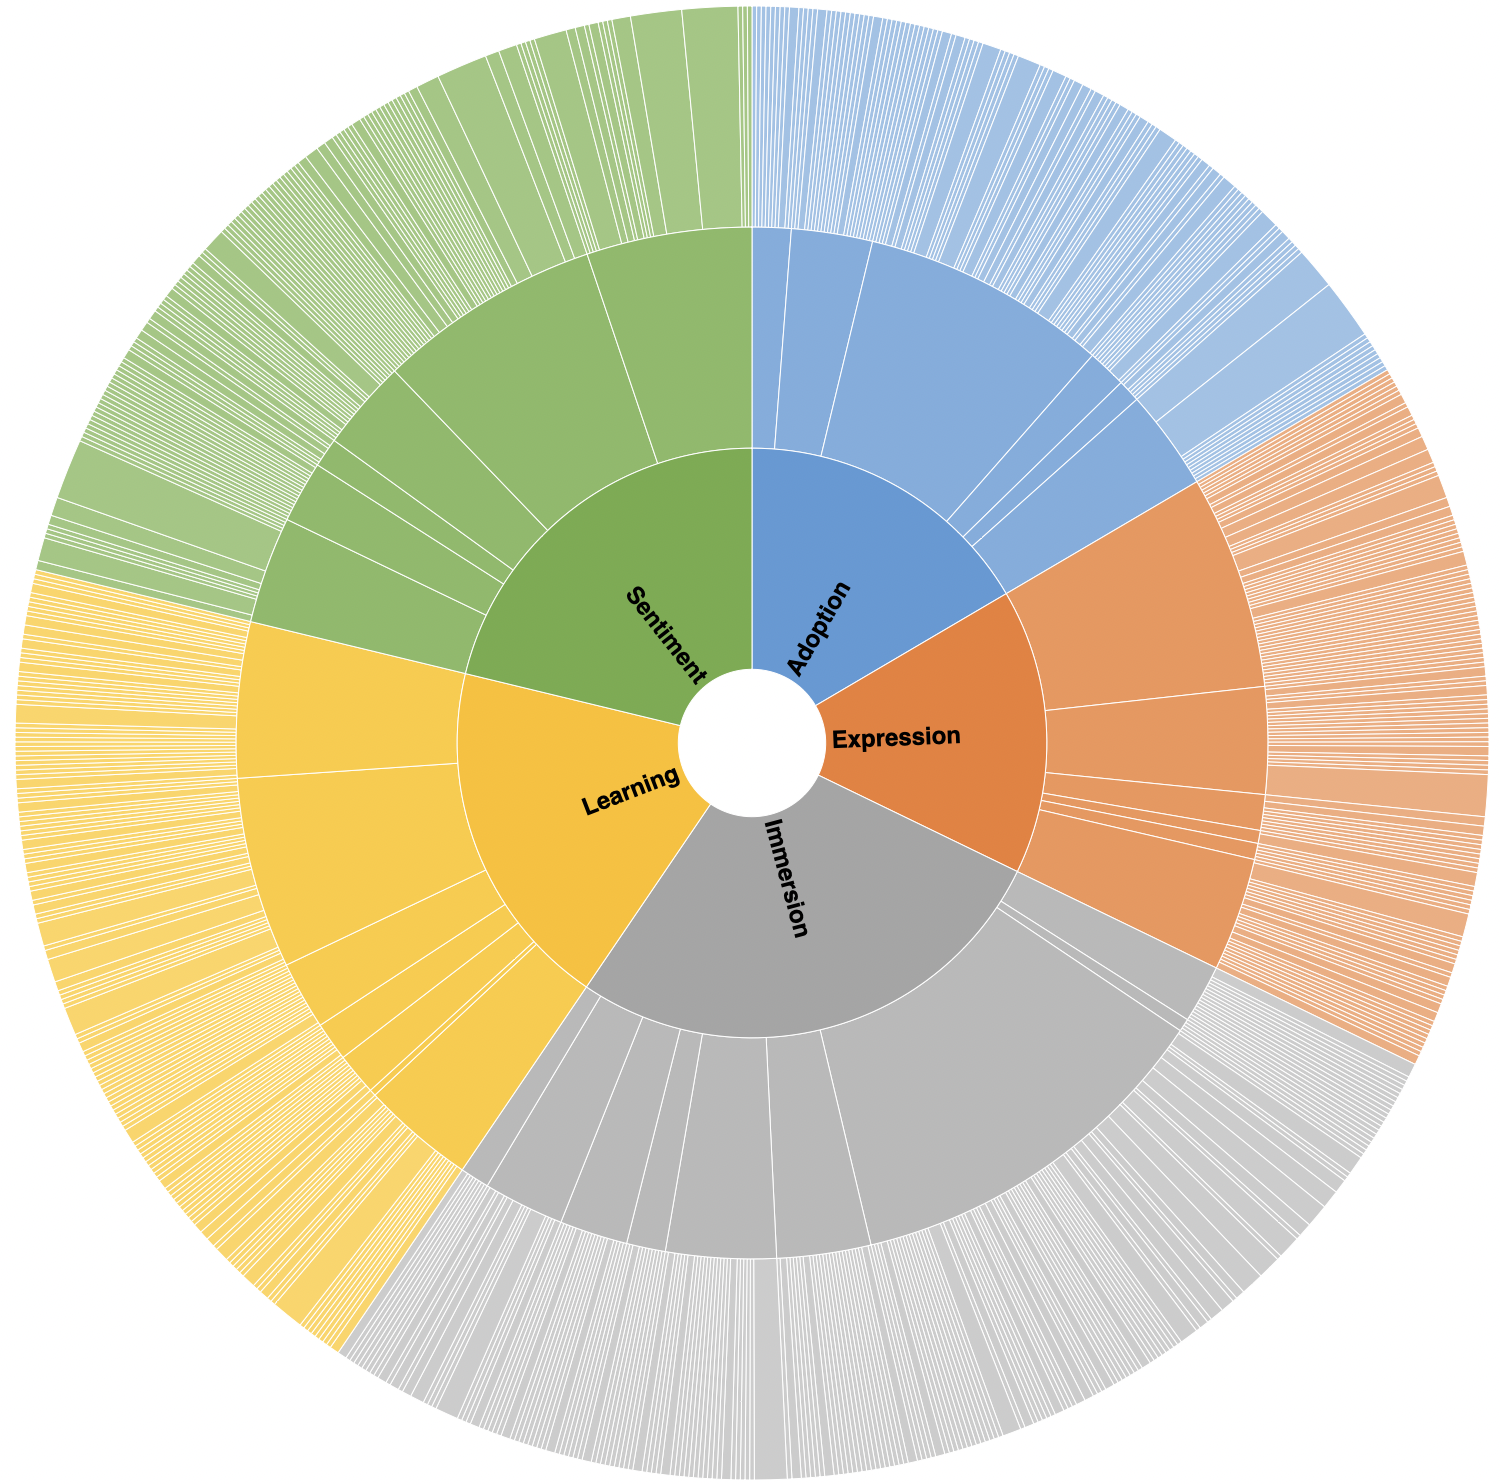
\includegraphics[width=0.7\linewidth]{figures/06-polaris/polaris-feedback-grounded-codes.png}
    \caption{5 categories, 37 subcategories and \textasciitilde{}700 codes visualised in NVivo.}
    \label{fig: polaris-feedback-grounded-codes}
\end{figure}

Transcribing the nearly 7 hours of experiences and interviews, lead to 45,858 words, and approximately \textasciitilde{}700 individual codes in the qualitative research software NVivo. These were sorted into 37 subcategories, with a total of 5 categories.

\subsection{Sentiment}\label{sec: polaris-feedback-sentiment}
Included in this category are emotions elicited by the experience, the majority of which were related to novelty. Participants felt a mixture of emotions, most frequently wonder or awe at the visual components of the scene, and enjoyment of the scene components and the interactions with them.

One participant felt fixated by the experience: \textit{`I am quite obsessed by this button'} (P9), whilst another felt satisfaction: \textit{`Like a fascination, wonder, it was quite satisfying as well'} (P3).

All participants made ample use of simile and metaphor, likening visual elements to liquid, snow, fire, fireworks, magic, and confetti. The sound design was said to be \textit{`ocean-like'} (P7) or \textit{`wind-like'} (P1), and participants expressed similarities in their experience to `being in' movies such as \textit{Star Wars, Minority Report, and Enter the Void} - \autoref{fig: films}.

\begin{figure}
    \centering
    \captionsetup{justification=centering, margin=1.5cm}
    \subcaptionbox{`The Force' \citep[in][]{kershner1980}}[.3\linewidth]{\includegraphics*[height=2.75cm]{06-polaris/kershner1980.png}}\label{fig: kershner1980}
    \hfill
    \subcaptionbox{Mid-Air Displays \citep[in][]{spielberg2002}}[.3\linewidth]{
\includegraphics[height=2.75cm]{06-polaris/spielberg2002.png}}\label{fig: spielberg2002}
    \hfill
    \subcaptionbox{Psychedelic Visuals \citep[in][]{noe2009}}[.3\linewidth]{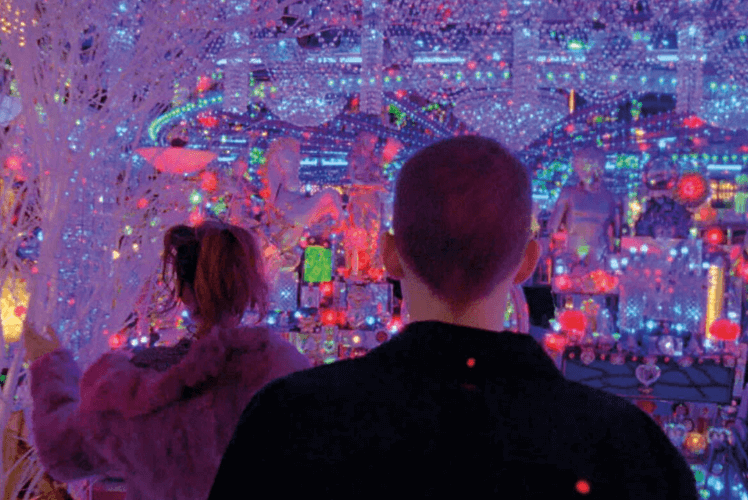
\includegraphics[height=2.75cm]{06-polaris/noe2009.png}}\label{fig: noe2009}
    \caption{Participants likened the experience of polaris\textasciitilde{} to `being in' Star Wars, Minority Report, and Enter the Void}\label{fig: films}
\end{figure}

\subsection{Learning}\label{sec: polaris-feedback-learning}
From this category of codes, is clear that the experience involved an element of learning different functions and abilities. One participant remarked: \textit{`I was unsure, and I didn't know what would lead to a change in what I did, but after a point I understood'} (P6). Another linked learning as resulting in immersion: \textit{`Each step that you learn something new about what you can do in that environment, that's when you become more and more immersed'} (P9).

\subsection{Adoption}\label{sec: polaris-feedback-adoption}
This category includes codes that referred to issues that could be a barrier to using the technology, recommendations for different utilisations of audiovisual AR, and codes relating to safety and accessibility implications of adopting AR.

\subsubsection{Comfort and Fit}\label{sec: polaris-feedback-adoption-comfort}
8 out of 10 participants struggled with the fit of the headgear on the Project North Star not being tight enough. As a result, some participants had to hold the headset with one hand throughout the experience. One participant expressed that this \textit{`stood as a hurdle to [the] experience'} (P1), and another specified how this affected their involvement with experience in more detail: \textit{`[Discomfort] doesn't ruin it, but it definitely brings me back to reality really quickly'} (P10).
\subsubsection{Alignment and Tracking}\label{sec: polaris-feedback-adoption-alignment}
Related to the above, were codes that referred to issues with alignment of content onto the real environment, such as the floating orbs and the outline of the hands. These were a product of the sensors, lighting, and content of the lab space. One participant even described the slight delay and misalignment of the hand outline as \textit{`trippy'} , going on to say that they \textit{`sort of like that it's a bit out'} (P1).

\subsubsection{Uses of AR and comparisons to other media}\label{sec: polaris-feedback-adoption-uses}
A wide variety of possible uses of audiovisual AR were highlighted by participants, including communication, conveying certain messages by highlighting important subject matter, art and music, virtual worlds, and video games.
One participant, who studies Media for Development and Social Change and works with environmental NGOs, remarked that using audiovisual AR could help generate more interest in environmental conservation, because experiencing AR made them feel \textit{`for some reason I act like this [virtual content] is more real than it is'}, going on to say that \textit{`rather than just watching it on the screen, you'd be more integrated'} (P6).

Another participant, studying on the same course, considered the use of AR in the documentation of the lived experiences of vulnerable people, such as refugees. They emphasised that compared to traditional media formats, AR was more \textit{`interactive'}, and that this could help in \textit{`angling the participant to be in touch with the subject more'} (P1), possibly helping raise awareness of vulnerable people without tokenising their lived experience.

Several other participants described the potential uses of AR in artistic and musical contexts like \textit{polaris\textasciitilde{}}. One participant said that AR had the potential to allow musicians to \textit{`easily feel'} and \textit{`play [...] with sounds'} (P2). One participant said that they could see AR being used for both instrument-building and creating installations (P3).

\subsubsection{Safety and Accessibility}\label{sec: polaris-feedback-adoption-safety}
On the topic of safety, one participant expressed that despite \textit{`[feeling] like there will be lots of benefits for [the uptake of AR and VR]'}, they believed that it could lead people to \textit{`lose track of reality'} (P7). Overall, participants reacted positively to the fact that their concerns over the comfortability and fit of the headset would be able to be addressed thanks to the open-source nature of the North Star's design.

\subsection{Expression}\label{sec: polaris-feedback-expression}
Participants expressed themselves in various ways during the AR experience, and most described the ability to create visual and sonic components with their hands as the most compelling aspect of this expression. For example, one participant appreciated the variety of visual and sonic patterns that they could create: \textit{`when your hands are together, it made one style of shape, and when your hands were away it would make different styles that affected the music'} (P7), another emphasised variety as well as exploration: \textit{`[The experience] let me explore by using my hands [and] doing different gestures'} (P6).

[iframe element]

Accordingly, several participants expressed their ability to act in the scene as \textit{`control'} or \textit{`power'}. One participant, almost sounding guilty, said: \textit{`I mean, it sounds weird, but I felt, like, very powerful'} (P10). Another, remarked similarly: \textit{`I think once I realised that I had the power to add things, I didn't let go of that'} (P3).

While one participant remarked that \textit{`physically doing something [that] you can see the effect of'} resulted in a feeling of \textit{`control'} (P7), another participant noted that they didn't always feel this: rather, that this might grow over time and with increased familiarity of the scene, reinforcing the suggestion of a learning process in the experience (P3).

Closely related to these codes were ones where participants expressed their wish to have more power and control over the scene, or that they had wished for different outcomes. Most common was the wish to be able to move the orbs around themselves (P3, 6, 9) or the ability to change elements as I had done in the experimental part of experience themselves, and at their own leisure (P5, 7, 9, 10).

One participant agreed that adding further visual indicators for the effects being had on the sound would help them notice these changes. The same participant commented that the pinching gesture used to tighten the stream of particles from the hand was unintuitive and would have preferred it to be a pointing gesture (P2).

\subsection{Immersion}\label{sec: polaris-feedback-immersion}
\subsubsection{Awareness}\label{sec: polaris-feedback-immersion-awareness}
Most participants reported that they felt aware of their real-world surroundings during the experience, one commenting that it was \textit{`because you could still see everything, you could still hear'} that they didn't get \textit{`lost'} in the experience (P7). However, one of the participants was adamant that they had \textit{`lost track of reality'} during the experience, and that it had felt \textit{`like [they were] in another environment'} (P9), another still, observing that there were moments when they forgot where they were (P10). It's clear then, that the experience immersed the participants, some more than others. When asked to offer a rationale for their feelings of immersion, participants pointed to several factors.

\subsubsection{Sights}\label{sec: polaris-feedback-immersion-sights}
One participant noted that they felt more immersed by the visual components of the scene, but that they would have felt less immersed if there wasn't an auditory component to the experience (P10). When being immersed by visual elements, for some it was colours that maintained this sense of immersion, with one participant commenting that the \textit{`vividness'} (P8) and size of the colours when particles had been made larger in the experimental section is what led to the moments of highest immersion in their experience.

\subsubsection{Sounds}\label{sec: polaris-feedback-immersion-sounds}
On the topic of immersion through audio, one participant put this down to the feeling of being \textit{`submerged'} in different layers of three-dimensional sound (P1). Similarly, many of the participants confirmed or independently reported to be able to discern and localise the tones they heard from different orbs around them, with some doing this by exploring through movement (P7), and others taking the visual cue of the white particle burst (P3). One participant remarked that the sound was the \textit{`main aspect'} of immersion for them, and that it made them \textit{`feel like part of'} the experience (P4); another commented that the sound \textit{`surrounded'} them and held their concentration so much that they almost forgot that they were wearing the bone-conduction headphones (P2). For another still, it was the activation of one of the orbs' sound effects that made them feel part of the experience (P3).

\subsubsection{Actions}\label{sec: polaris-feedback-immersion-actions}
A participant remarked that it was the feeling of \textit{`creating'} that led to their immersion. Additionally, they remarked that it was the \textit{`element of play'} in the interaction between particles and orbs that had immersed them in the experience; further noting that it was the way that the particles \textit{`emerged'} from their hands that kept them engrossed (P9). On playfulness and fun, another participant commented that it was the fact that they could interact with content that wasn't \textit{`there'} which was the most fun for them (P5).

\subsubsection{Physicality of Content}\label{sec: polaris-feedback-immersion-physicality}
One participant reported multiple times that they could \textit{`feel'} the button when they pressed it (although technically it was floating adjacent to their hand in mid-air). They agreed that it could be the mixture of the feedback sound, volumetric threshold trigger, and lighting that led to this effect (P9).

Another participant, upon placing their hands close to an orb remarked: \textit{`I know there's nothing there, but when I put my hand [towards the orb] I feel like I'm going towards something warm'}. This same participant expressed a keen interest during the experimental section in drawing large three-dimensional sculptures. During one of these drawings, the participant walked around their creation, and then took a moment before exclaiming: \textit{`Oh! I forgot that it wasn't a real thing, I kept trying to go [around] it, but I could just go through it!'}. Later, they noted: \textit{`I guess it's about our brains. [...] When we see it in 3D we automatically think it's more real than [if it were on a screen]'} (P8).

% --------------------------------------------------------------------------- %
\section{Conclusion}\label{sec: polaris-conclusion}
Overall, the AR experience engaged participants fruitfully, with many noting their ability to express themselves audiovisually in creative ways. For \textit{polaris\textasciitilde{}}, the ability to do so whilst maintaining a privacy-respecting and cost-effective focus, is a testament to the individual components of the framework used to create it, and the labour that has facilitated the development of these open-source solutions.

The categories of codes extracted from the grounded theory analysis have resulted in a rich set of data. From those related to participant sentiment, it's not only clear that the audiovisual AR experiences are able to elicit a wide variety of emotions, but that to explain and make sense of them participants often made use of metaphors and past experiences. The fact that it was expressed multiple times by participants that the experience was one that they'd never had before might be a way of accounting for this variety and overlap of emotions.

Relating to the category of learning, it's clear that participants sensed this from multiple aspects of the experience, with one pointing towards the dimensionality, and others pointing towards the interactive elements and the need to explore the scene. For one participant there was a connection between learning and immersion. Within the context of musical interfaces, this could be taken to show that viewing the participant as a learner in the experience could lead to a deeper level of engagement.

Within the category of adoption, the fact that the headset lacked a good fit for most participants was clearly what detracted from the experience most. It led not only to a reduction in experience immersion, but also to a lessening of comfort and the knock-on effect of muscle fatigue and inability to exercise full agency for some participants. From the comments on different potential applications for AR, it is clear that the offer of deeper interaction with subject matter, increased immersion in an experience, and the sense of \textit{`feeling'} or \textit{`playing'} with virtual content has led to participants envisaging AR's utilisation in several artistic and musical contexts. Notable was the suggestion that these facets of experience, especially that of the three-dimensional and context-specific sounds, could be employed to convey messages of socio-ethical importance as well as aesthetic experience. It is important to mention that some participants warned of negative side-effects or the potential for negative experiences in AR, showing the importance for a safety-minded approach to designing such AR experiences.

From the codes relating to self-expression and control, participants appreciated the ability to interact with their bare hands, and felt that this was the main contributor to their expression in the scene. This, for some, led to a feeling of power, and for some, a feeling of control over elements of the scene. For others, the feeling of control wasn't entirely certain, with some noting that the scene had agency of its own. It is also conclusive from these codes that some participants desired more control over the scene, although implementing this would have to be done thoughtfully, without overloading the scene with content and parameters to change.

Immersion tended to stem from the fact that the elements of the experience: sights, sounds, and actions were spatialised in three dimensions. Participants enjoyed and felt immersed by the movement and colour of the visual elements and were able to discern and localise the source of different sounds in the experience; several noting that this element was the most immersive factor for them, whilst others preferred the visual elements. Others still, noted that the actions that they employed, gestural and movement-based are what immersed them in the experience most, and for some, this led to the virtual content of the scene feeling physical at times.

[iframe element]

While the above analysis is not, on its own, sufficient to draw conclusive guidelines for design, it does shed light on several connections between elements of this specific experience: learning, comfort, safety, spatial perception, visual-, sonic-, and action-led immersion, and physicality of virtual content. In \autoref{sec: discussion-medium} this is expanded upon, and this has lead to the iteration of parts of the design patterns found in \autoref{sec: discussion-patterns}.

[iframe element]

To improve on the comfortability of the experience, the first changes I made were to design an alternate headgear section for the headset. Over the course of a day, I collaborated with another NS community member on \href{https://github.com/AheadIO/Deck-X/tree/main/Deck_X/STL_files/Headgear/Welding_Headgear_Adaptor}{3D printable designs} that would allow the quick and easy substitution of the main headgear piece for a smaller one that was more accommodating of smaller head sizes.

I would also like to make the gestures and feedback for the orb-based sound effects more intuitive, reachable, and musical, as most participants relied on my showing them before they understood that it was a possibility in the scene. This could be done by conducting a trial with musician participants with which to iteratively develop these new interactions. 

On the basis of the codes related to learning, I would like to experiment with an implementation of increasingly interactive and musical \textit{`levels'}, both to reduce overwhelm when starting the scene, and to provide participants with a simple course through which to learn functions and express themselves accordingly.
  \clearpage% --------------------------------------------------------------------------- %
%                   __                      _                                 %
%  _ __   ___ _ __ / _| ___  _ __ _ __ ___ (_)_ __   __ _                     %
% | '_ \ / _ \ '__| |_ / _ \| '__| '_ ` _ \| | '_ \ / _` |                    %
% | |_) |  __/ |  |  _| (_) | |  | | | | | | | | | | (_| |                    %
% | .__/ \___|_|  |_|  \___/|_|  |_| |_| |_|_|_| |_|\__, |                    %
% |_|                                               |___/                     %
%                                         _                                   %
%                             _ __   ___ | |_   _  __ _  ___  _ __  ___       %
%                            | '_ \ / _ \| | | | |/ _` |/ _ \| '_ \/ __| /\/| %
%                            | |_) | (_) | | |_| | (_| | (_) | | | \__ \|/\/  %
%                            | .__/ \___/|_|\__, |\__, |\___/|_| |_|___/      %
%                            |_|            |___/ |___/                       %
% --------------------------------------------------------------------------- %
\chapter{Performing polygons\textasciitilde{}}{Developing a Sound ARt Performance Practice}
\label{sec: polygons}
%\markboth{}{Performing polygons\textasciitilde{}}
\epigraph{\emph{Our environment is not a play, a performance in which only minor modifications are possible. It's an improvisation,[…] the nature of the interaction is radically open.}}{\citep{vermeulen2015}}

\noindent \textbf{polygons\textasciitilde{} Blog:}        \url{https://www.sambilbow.com/projects/polygons}

\noindent \textbf{polygons\textasciitilde{} Code:}        \url{https://www.github.com/sambilbow/polygons}

\noindent \textbf{polygons\textasciitilde{} Guide:}       \url{https://www.github.com/sambilbow/polygons/wiki}

\vspace*{2cm}

\begin{figure}[!ht]
    \centering
    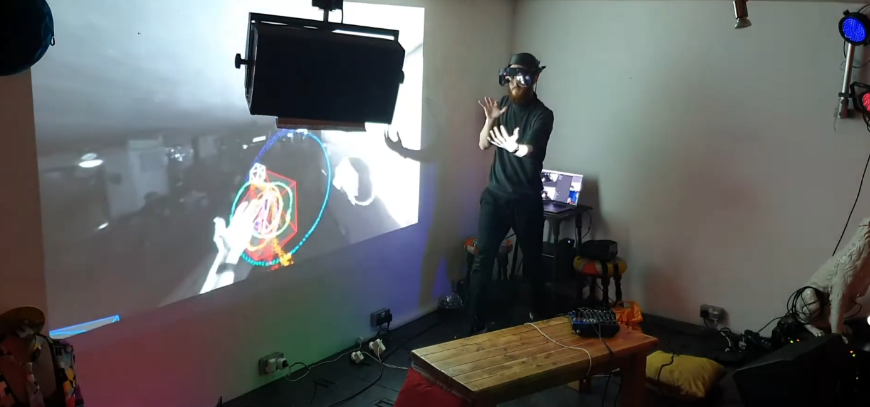
\includegraphics[width=0.7\linewidth]{07-polygons/polygons-ambi-rh.png}
    \caption{Performance of \textit{polygons\textasciitilde{}} at The Rosehill}
    \label{fig: polygons-ambi-rh}
\end{figure}

\clearpage
% --------------------------------------------------------------------------- %
\section{Summary} \label{sec: polygons-developing}
As a direct consequence of witnessing participants enjoyment and play with \textit{polaris\textasciitilde{}}, I recognised for the first time looking from the outside in, that the system had a larger propensity for fostering learning, virtuosity, and depth of expression than I had originally thought; if only the experience was slightly more complex, the interactions more \textit{nuanced}. The gestures, play, and expression by participants led to a kind of quasi-transhumanist dance, one that struck me as a technologically mediated dialogue between hybrid self and hybrid environment, a delicate balance of agency.



Until this point, I had been primarily focused on the medium as used for the composition of musical pieces e.g. \hyperref[sec: area]{\textit{area\textasciitilde{}}}, or of installation-like experiences \hyperref[sec: polaris]{\textit{polaris\textasciitilde{}}}. Performance with AR had remained abstract, especially as, formally, its not my preferred mode of musical expression. However, the balance of agency between participant and system, between self and environment, presented itself during the evaluation of \textit{polaris\textasciitilde{}} to be an area ready for exploration through performance. 

The following chapter outlines my exploration of a a fifteen-minute experimental audiovisual AR improvisation using an AR performance ecosystem called \textit{Weird Polygons and Hand Noises}, or \textit{polygons\textasciitilde{}} for short.



% --------------------------------------------------------------------------- %
\section{The Composition of \textit{polygons\textasciitilde{}}} \label{sec: polygons-composition}

%*[ ]   What?
Drawing from the categories extracted from \nameref{sec: polaris}: \nameref{sec: polaris-feedback}, I pursued the design of a system with physically moveable elements, audio-reactivity, and enough room to be able to learn and explore the scene both spatially and in terms of interaction and sonic palette. Thus, as an AR performance ecosystem, \textit{polygons\textasciitilde{}} delivers this by describing the improvisational and performative relationship between a performers actions via body, hand, and head movement, feedback from the audience, and three real-time AR musical instruments: \textit{ambi}, \textit{click}, and \textit{hands}. 

%*[ ]   add unity image of ambi w/ particles
\textit{ambi}, a red wire-frame icosahedron, serves as a dual-oscillator drone synthesiser that the performer can call on my taking and bringing it closer to them with their hands. Its voice is contingent eleven real-time parameters, which are sent to the PureData patch attached to it. At specified distance two particle systems are activated from the palms of the performers hands, and the drone from \textit{ambi} is activated. The particles are drawn to the centre of \textit{ambi}, their paths guided by an unseen particle forcefield - the same behaviour as in \textit{polaris\textasciitilde{}}. Real-time hand `collision' in three dimensions with \textit{ambi} is constantly reported per hand, resulting in two sets of $x,y,z$ coordinates that form part of the data that is mapped to parameters in PureData (see \autoref{fig: polygons-ambi-mapping}).
\begin{table}
    \centering
    \begin{tabular}{ l|l l }
        \textbf{Unity Scene Attribute}  & \multicolumn{2}{ l }{\textbf{PureData Parameter}}   \\
        \hline
        \textbf{Hand}                   & \textbf{via Left Hand}& \textbf{via Right Hand}       \\
        \hline
        Collision Distance              & Drone 1 On / Off      & Drone 2 On / Off              \\
        Collision X                     & Reverb Amount         & Drone 2 LPF CF Mod            \\
        Collision Y                     & Drone 1 Pitch         & Drone 2 Pitch                 \\
        Collision Z                     & Rev/Dly Amount        & Drone 2 LPF CF                \\
        \hline
        
        \textbf{\textit{ambi}}          & \multicolumn{2}{ l }{\textbf{via pinch gesture}}    \\
        \hline
        Scale                           & \multicolumn{2}{ l }{Output Filter Cutoff}          \\  
    \end{tabular}
    \caption{The parameter mappings for \textit{ambi}}
    \label{fig: polygons-ambi-mapping}
\end{table}
%*[ ]   move panel in patch under each other for space
\begin{figure}
    \centering
    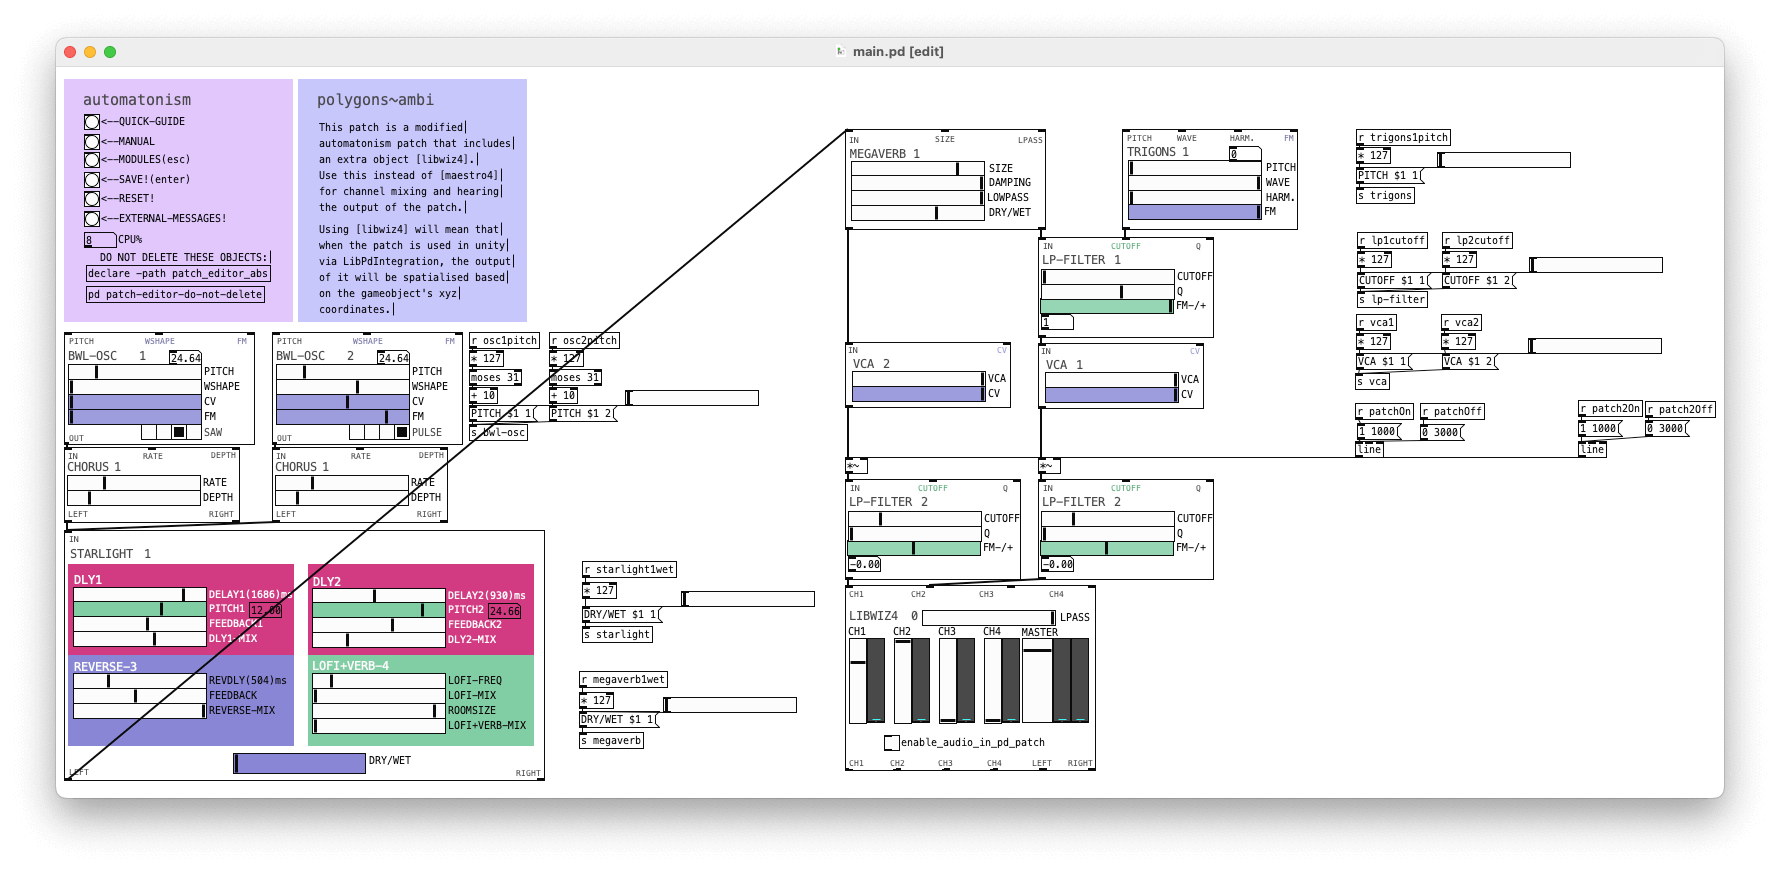
\includegraphics[width=0.7\linewidth]{07-polygons/polygons-ambi-pd.png}
    \caption{The PureData patch for \textit{ambi}}
    \label{fig: polygons-ambi-pd}
\end{figure}

%*[ ]   add unity image of click w/ particles
\textit{click}, a set of two blue wire-frame icosahedra, form a feedback system between two low-frequency oscillator controlled impulse generators. The feedback can be altered by bringing the smaller icosahedron (\textit{click-}) closer to the larger one (\textit{click+}). \textit{click+-} makes use of LibPdIntegration's Unity send functionality; each time there is an impulse generated, a message is sent to Unity, which triggers a shower of particles to be emitted from \textit{click-} to \textit{click+} forcefield-guided cone. As the performer intervenes and creates the feedback system, the closer they bring the icosahedra together, the faster the visual particle shower becomes, and the more erratic the impulse generators feedback on each other. A further sound parameter, connected to a reverb, is mapped to the amount spin \textit{click-} let go with by the performer. The sound palette explores a gradient from static electricity crackles to a sound akin toa car motor catching and revving up as the feedback increases.
\begin{table}
    \centering
    \begin{tabular}{ l|l }
        \textbf{Unity Scene Attribute}         & \textbf{PureData Parameter}   \\
        \hline      
        \textit{click+-} Distance              & Impulse 1 Frequency           \\
        \textit{click-} Collision X            & Impulse 2 Frequency           \\
        \textit{click-} Collision Y            & Impulse Chorus Rate           \\
        \textit{click-} Collision Z            & Impulse Chorus Depth          \\
        \textit{click-} Release Spin Velocity  & Impulse Reverb Amount     
    \end{tabular}
    \caption{The parameter mappings for \textit{click}}
    \label{fig: polygons-click-mapping}
\end{table}
\begin{figure}
    \centering
    \includegraphics[width=0.7\linewidth]{07-polygons/polygons-click-pd.png}
    \caption{The PureData patch for \textit{click}}
    \label{fig: polygons-click-pd}
\end{figure}

%*[ ]   add unity image of hand w/ colours
\textit{hands} constitutes the final AR instrument in \textit{polygons~}; each of the performers hands, when a virtual button besides their palm is toggled \textit{on}, generate a highly resonant filtered white noise. The cutoff, resonance, and amplitude of this generator-filter system is controllable independently per hand, through several dynamic movement-based attributes. The filter cutoff per hand is mapped to that hand's distance to the performer's face; the filter resonance per hand is mapped to the angle from that hand's palm angle towards the centre of the performance space; and the amplitude of each is mapped to the stretching of the fingers outwards away from the palm. The sounds delivered by \textit{hands} are harsh and unpleasant at certain parameter combinations and purposefully loud; from a performative standpoint, this engenders specific gestures, movements, and stances, as the performer grapples with a sonic experience akin to howling and shrieking winds.
\begin{table}
    \centering
    \begin{tabular}{ l|l }
        \textbf{Unity Scene Attribute}         & \textbf{PureData Parameter}    \\
        \hline      
        \textit{hand} to Head Distance         & Filter Cutoff                  \\
        \textit{hand} to Stage Angle           & Filter Resonance               \\
        \textit{hand}'s Finger Extension       & Amplitude               
    \end{tabular}
    \caption{The parameter mappings for \textit{hands}}
    \label{fig: polygons-hands-mapping}
\end{table}
\begin{figure}
    \centering
    \includegraphics[width=0.7\linewidth]{07-polygons/polygons-hands-pd.png}
    \caption{The PureData patch for \textit{hands}}
    \label{fig: polygons-hands-pd}
\end{figure}

Together, and separately, \textit{ambi}, \textit{click-+}, and \textit{hands} provide a complex sound palette, explorable by the performer through non-linear combinations of hand gestures, body movements, and stances, that themselves invariably feed back into the decisions made to delve into and combine specific sounds. Visually, \textit{polygons\textasciitilde{}} draws on the pioneering 3D wire-frame AR systems of the 20th century such as the \textit{KARMA} system \citep{feiner1993} and Sutherland's \textit{Ultimate DIsplay} \citeyearpar{sutherland1968} (see: \autoref{fig: polygons-wireframes}), which were a design choice constrained by computational power at the time. This is juxtaposed by the fluid and visually complex behaviour of the thousands of multicoloured particles used by \textit{ambi}, and \textit{click-+}.

\begin{figure}
    \centering
    \subcaptionbox{Sutherlands `Ultimate Display'}[.3\linewidth]{\includegraphics[height=2.5cm]{07-polygons/sutherland_68.png}}
    \subcaptionbox{Feiner's `KARMA' System}[.3\linewidth]{\includegraphics[height=2.5cm]{07-polygons/feiner_93_2.png}}%
    \caption{Wire-frame Influences}
    \label{fig: polygons-wireframes}
\end{figure}


% --------------------------------------------------------------------------- %
\section{The Performance of \textit{polygons\textasciitilde{}}} \label{sec: polygons-performances}
\subsection{\textit{polygons\textasciitilde{}}Technical Setup} \label{sec: polygons-performances-setup}
From a system design perspective, as with any instrument, the importance of the performer's aesthetic experience as described the the previous section is indubitable; most of the software and hardware I had used in the development of \textit{polaris\textasciitilde{}} was readily transferable to the context of performance. There was no need to change from the combination of PureData, LibPdIntegration, and Unity. However, when considering the design of an AR experience \textit{as} performance, there began to surface new design considerations that needed answers:
\begin{itemize}
    \item \textit{By what means could I invite an audience into the hybrid space I was creating with \textit{polygons\textasciitilde{}}?} 
    \item \textit{What elements of my experience would / could be shared with an audience?} 
    \item \textit{How could I go about performing an experience that I was, by now, intimately aware of, but would be difficult without context for an audience to understand?} 
\end{itemize}
Due to time constraints, the performance system I decided on was fairly simple. For translating my visual experience (I deemed this necessary for the audience to understand my gestures and their links to musical outcomes) I would project the real-time hybrid composite feed (made up of a black and white video feed from one of the head-mounted sensors on the headset with an overlay of the Unity scene) on the wall behind me. For the audio, I replaced my bone-conduction headphones (sacrificing some of my own 3D audio immersion) with the PA system of the venue. The panning would be reversed so that my gestures and movements would translate realistically to the audiences auditory perspective, i.e. the movement of my hand during the performance of \textit{hands} across my body from left to right would transfer to the sound panning house-right to house-left rather than stage-left to stage-right.

\subsection{The Rosehill - February 2022} \label{sec: polygons-performances-rosehill}
\textit{polygons\textasciitilde{}} was developed for a performance as part of the seventh Experimental Music Technologies (emute) Lab \href{http://www.emutelab.org/blog/emutelab6}{showcase} at The Rosehill - an independent venue, recording studio, label, creative hub, and co-working space run by artists and musicians. The recording of the performance is hosted online, and can be found on the \textit{polygons\textasciitilde{}} \href{https://github.com/sambilbow/polygons}{GitHub repository}. The Rosehill performance was the first time I had immersed myself in the \textit{polygons\textasciitilde{}} system for an extended period of time; I had held off extended use of the system during prototyping the instruments. This lead to an authentic exploration and improvisation of the material, embodied, and spatial affordances of the three instruments, \textit{ambi}, \textit{click-+}, and \textit{hands}. The combination of sharing the audiovisual elements of my experience, auditory immersion of the audience, and performing through improvisation, led to an intimate performance. In itself, this decision was also an improvisation, I had not practiced or rehearsed, and this was my first performance of a non-traditional instrument. This took the form of me taking it upon myself to `showcase' the instruments to the audience, through a kind of theatrical and gestural dance that the audience were invited to be part of. 

One issue I hadn't anticipated was strobe caused by feedback between the visuals behind me and the sensor cameras in the headset when I stood in the throw of projector. This combined with the otherwise darkness of the room lead to a few moments where the sensors on the headset momentarily lost calibration, moving the Unity scene contents slightly. Whilst I (and study participants) had experienced this during \hyperref[sec: polaris-feedback-adoption-alignment]{\textit{polaris\textasciitilde{}}}, due to the confines of the stage, and the wall behind me, this did present slightly more of a problem and limited my performance space somewhat. For example, when \textit{click-} moved behind the wall, forcing me to stand flush with the wall and try very hard to take it out (\href{https://youtu.be/9IErsDvhXjM?t=210}{03:30}). This wrangling between the virtual and physical space presented itself as a comedic moment for the audience, and was a moment of where the mechanics of the hybrid space became obvious, and relatable despite the distance between the audience and my own understanding and experience of AR. Overall though, the performance, despite its hitches was received extremely well, with members of the audience afterwards exclaiming that they'd never seen any such kind of performance. 

\subsection{Showcase at the ACCA - June 2022} \label{sec: polygons-performances-acca}
\textit{polygons\textasciitilde{}} was performed three months later at an end-of-year departmental showcase at the Attenborough Centre for the Creative Arts (see \autoref{fig: polygons-acca}). The space here was much larger, allowing me more space to explore (although still limited by the length of the headset cable - 2.5 metres), it reduced the chance of the aforementioned strobe, which made the sensor alignment more stable.

\begin{figure}
    \centering
    \includegraphics[width=0.7\linewidth]{07-polygons/polygons-acca.png}
    \caption{\textit{polygons\textasciitilde{} performance at the ACCA}}
    \label{fig: polygons-acca}
\end{figure}

\subsection{Demonstrations - May \& June 2022} \label{sec: polygons-performances-demos}
For furthering understanding of AR as a medium for artistic and musical practice, as well as for providing novel experiences to those who hadn't experienced AR yet, \textit{polygons\textasciitilde{}} was made open for students and faculty to perform and experience as part of the first MAH Doctoral Conference. It was also open for experience as part of the SHL Make \& Create day, on the 25th of May, and 9th of June 2022 respectively.

These sessions provided a chance to glean some face-to-face informal feedback on the design, rationale, and sound-world of \textit{polygons\textasciitilde{}}. Not to mention, it was an exercise in seeing second hand the amount of embodied knowledge, and skilful AR know-how I had accumulated with the system I had used for 18 months by this point. Those experiencing XR for the first time definitely struggled more with the gestures needed to move, resize, and interact with the three instruments.



% --------------------------------------------------------------------------- %
\section{The Future of AR Sound ARt Performance}
From the performance of \textit{polygons\textasciitilde{}}, it became clear to me that AR within a musical performance practice can be an effective medium for the creation of novel aesthetic experiences for performer \textit{and} audience. However, improvements could be made to the process of `inviting' the audience into the performer's hybrid space. \textit{polygons\textasciitilde{}} in this regard, was fairly unpolished, even for a first performance - and I imagine the audience felt as if they were `witnessing' rather than `experiencing' with me. Therefore, I envisage the challenges for future AR musical performances in my own, and in the broader community's practices, lying in the development of immersive audience experiences.

 With the exception of the incredible work by Amy Brandon using the METAVision headset \citeyearpar{brandon2018}, I have been hard-pressed to find other live audiovisual performances that specifically appropriate AR \textit{headsets} as their actual medium of performance. Despite there being an array of cutting edge performances that use AR technologies in their execution, it is extremely new as a research area, with a lot of exploration and research to be done. Like in most aspects, due to the amount of funding and earlier research focus, VR has been an area where artistic and musical performance has flourished in the last 20 years, with early pioneers \citep{davies2004} paving the way for the consideration of the body in immersive 3D space. \textit{polygons\textasciitilde{}} could be closely linked to contemporary VR visual art making practices, where artists sculpt, paint, and draw in 3D in an infinite world canvas \citep{summers2019}. AR musical performance however, is beginning to gain traction, with participatory installations \citep{chevalier2018},  projection-based performances \citep{quay2016,berthaut2016,robinson2020}, tangible AR projects \citep{zamborlin2018}, and real-time notation techniques \citep{santini2020,santini2022}. 

As found in the field of spatial acousmatic performance \citep{sharma2015}, a clear vocabulary ought be developed here due to the wide disciplinary scope of the technologies, aesthetics, and modes of performance explored. Indeed, the public perception of `AR performances' has typically come to describe the use of AR as the \textit{medium of playback} -- replacing the 2D screen with an immersive 3D viewing/listening of a live or pre-recorded musical experience -- rather than the \textit{medium of performance}.

\textit{polygons\textasciitilde{}}, like any prototype instrument or performance, has therefore asked more questions that it has answered. Concerning the future of AR musical performance, the present thesis proposes the following questions as potential research avenues:
\begin{itemize}
    \item Can we avoid `spectacle' of AR? How else can we meaningfully engage audiences who are new to AR?
    \item How can we invite the audience into AR musical performance more effectively?
    \item Is wearing more technology necessarily the best avenue for a focus on embodied performance?
    \item What would an AR ensemble look, sound, and feel like for both performer and audience?
    \item Could AR be appropriated for real-time networked performance of physically separate spaces?
\end{itemize}
  \clearpage% --------------------------------------------------------------------------- %
%      _ _                        _
%   __| (_)___  ___ _   _ ___ ___(_) ___  _ __
%  / _` | / __|/ __| | | / __/ __| |/ _ \| '_ \
% | (_| | \__ \ (__| |_| \__ \__ \ | (_) | | | |
%  \__,_|_|___/\___|\__,_|___/___/_|\___/|_| |_|
% --------------------------------------------------------------------------- %
%*[ ]   Draft design patterns
% --------------------------------------------------------------------------- %
\chapter{Implications for the Sonic Medium}
\label{sec: discussion}
\markboth{}{Implications for the Sonic Medium}
\epigraph{\emph{Alice has stepped through the looking glass [...] It is the job all future artists and activists to use this technology for the better, to bring people together, and uproot social injustice.}}{\citep[]{skwarek2018}}
% --------------------------------------------------------------------------- %
\section{From Overlay to Instrument} \label{sec: discussion-review}
The present thesis began in \autoref{sec: review} with an exploration of the landscape of historical and contemporary AR research and development spanning the past thirty years. Common forms, such as headset-, handheld- and projective-based AR were outlined, as well as typical sensory displays, allowing interaction and feedback with the visual, auditory, touch-based, and smell and taste senses. Furthermore, the processes by which AR mediates reality were laid out using Schraffenberger's categorisation of relationships and AR subforms: augmented, diminished, altered, and hybrid reality, as well as extended perception \citep{schraffenberger2018}. Despite this wealth of possible avenues for AR experience composition, the paradigmatic form of AR we hear about or see are predominantly characterised by being \textit{visual displays that overlay information}. Thus far in the thesis, this has been referred to as ocularcentric layering paradigm, or typical AR. This can be explained by a number of phenomena, but examining the origination of AR in the military-industrial complex by way of U.S Defence funding, it is not a surprise. This has had a compounded effect on the forms that AR finds itself being co-opted for in the arts. Several creative and expressive works were explored, that engaged in AR because of its ability to sensorily engage participants, induce rich aesthetic experience, enable collaborative expression, and empower new forms of agency and activism. Nonetheless, there are but a few examples of sound art AR experiences in comparison to visual counterparts because of the typical form of AR.

In proposing the development of AR as a medium for the creation of immersive sound artworks, its use as an instrument, or tool for sound art installation, I drew on several areas of importance in \autoref{theory}, first aesthetic experience and the `4E's', and then materiality, embodiment, and space. It began with a grounding in the concept of 'art as experience', drawing from the work of \citep{dewey1934}. Dewey states that the capitalistic reverence of fine art, notably by the "nouveau riches", has led to art being put on a pedestal - disconnecting it from its origin and operation in the everyday experiences of people. Leddy and Puolakka have since proposed that "material of art should be from all sources and art should be accessible to all" \citeyearpar{leddy2021}. Dewey points towards the aesthetic experience that art entails, and notes that the "live creature" is inseparable from the environment in which they are embedded. Today, despite social media as a platform for cultural production of artistic works has some merits, the fabric on which it is built is no different from the capitalist mechanisms that separated art from experience in the first place. Thus, open-source, hacker, DIY, and maker approaches were proposed as a method of democratising "all sources" of art, and attempting to increase accessibility. The focus on the body by Dewey also points towards the move towards tangible interface development, participatory design, and human-centred design that were outlined in \autoref{sec: method-resistance-maker}.

To delve deeper into this experience of art, I proposed an enactivist approach to considering cognition in experience. Often called 4E cognition (4EC), it states that cognitive process are embodied, embedded, enactive, and extended \citep{gallagher2017}. In considering the design, performance, and experience of AR, 4EC offers a fresh perspective on concepts such as agency, action, perception, immersion, and space.

The first theoretical lens through which to examine AR's design in computational art and music practice involved outlined the importance of a complex systems framing of interface use and performance. I drew on existing research from the field of digital musical instrument design \citep{magnusson2009a,discipio2003,essl2006,armstrong2006,hayes2019,chevalier2018} in order to demonstrate the usefulness of considering the material of performance systems as complex, and ecosystemic. To examine what happens in the experience of participants, the second lens was one that took seriously the assertions of 4EC, namely that cognitive processes in experience are embodied, embedded, enactive and extended. I draw from multiple disciplines of similar theoretical and practical work in VR and AR to show how 4EC offers a novel framing by which to consider the experience of AR by participants, audiences, and performers. Closing out the trio of theoretical lenses, is a grounding of the aforementioned consequence of AR for the experience and construction of "space". I first critically examine the term "Metaverse" \citep{stephenson1992}. Its modern-day origin is in technologies like AR and VR, which in turn sprung from "deep within the military and Western - scientific - industrial - patriarchal complex" \cite{davies2004}, and its current operation has been heavily co-opted by cryptocurrency projects. Because of this, in its current state, the "Metaverse" is hardly fertile ground for the "live creature" to experience art "accessibly", and from "all sources" \citep{dewey1934,leddy2021}, indeed, it mirrors the exact profit and exploitation motive of the historical context it originated in.



% --------------------------------------------------------------------------- %
\section{Engaging in a DIY Approach to AR} \label{sec: discussion-method}
\subsection{Approach to Practice / Theory}
\subsection{Outline of Method}
\subsection{Limitations}
\subsection{Proto-Design Pattern}
% lead to study results



% --------------------------------------------------------------------------- %
\section{From Overlays to Instruments} \label{sec: discussion-medium}
\subsection[Augmented Materiality]{Augmented Materiality: The Relational Fabric of the AR(tistic) Medium} \label{sec: discussion-medium-material}
Core to my own approach is, as I'm sure is evident by now, is the centring of the idea of the processual nature of AR systems. What are the processes; when I say real / virtual processes what is it that I am trying to convey? Ocularcentrism and the additive layering paradigm have shifted discussion of AR systems towards an object-centred view of the ``reality" that they present, this effect is also present in VR \citep[]{hovhannisyan2019}. Instead, I argue that an AR object is not a static visual thing with marked boundaries, not in any meaningful way to the artist/designer at least. It must be thought of as an on-going and distributed component existing inside a dynamic web of experience and meaning; as such, any discussion of the contents or material of an AR composition ought to be considered through this lens. Even a single apparent `virtual object' that is in front of a participant is not \textit{just} that; it is an invitation, a handle, a real-time process by which a participant can be perceptually guided through sensorimotor action towards a specific aesthetic experience. This so called `object' might be part of a larger organised whole, a component of a room-scale musical experience for example, or an emergent property of a hidden set of complex conditions that have only just been met through the specific movements of a participants body. This, more holistic, view of AR processes allows for a more fruitful discussion of the types of experiences we can expect to craft as AR practitioners; and engages more critically with Schraffenberger's taxonomy of AR relationships.

Embedding Schraffenberger's fundamental relationships (\autoref{table:schraffenbergertaxonomy2}) within Di Scipio's notion of an "ecosystemic" musical interface, or Water's ``performance ecosystem``, i.e. viewing the AR process as a real-time network of interactions distributed across the `hybrid' brain - body - environment, helps us in identifying the medium specificity of AR, and how it may uniquely be exploited to create meaningful AR artwork. If the motive for the composition of an artwork is to intentionally impart knowledge, meaning, or truth through aesthetic experience these must exist within and across the above network of interactions and relationships in our brain - body - environment distribution. I suggest we view this latent aesthetic experience as an real-time interaction between the components of:
\begin{itemize}
    \item Intention - the intended meaning behind the composition of the piece
    \item Medium - the specificity of the apparatus by which this meaning is imparted
    \item Experience - the on-going process by which the medium is engaged with by the participant
    \item Realisation - the resultant knowledge, truth, or subjective experience from of the above
\end{itemize}

\begin{table}
    \centering
    \begin{tabular}{ l l }
        \toprule
        Relationship        & Description                       \\
        \midrule
        Coexistence         & Unrelated                         \\
        Presence            & Spatially Related                 \\
        Information         & Content-Based Relationship        \\
        Physical            & Affect Each Other                 \\
        Behavioural         & Sense and React to Each Other     \\
        \bottomrule
    \end{tabular}
    \caption{Schraffenberger's Fundamental Relationships}\label{table:schraffenbergertaxonomy2}
\end{table}
In the first section of this chapter, we proposed that from Dewey's perspective, an artwork ought also to originate and operate within everyday sociocultural life in order to bring about positive social change through aesthetic experience. These concerns could be conceived as mainly arising from the component of intention, and its dynamic interaction through the medium into experience. Concerning the physical, or indeed virtual, manifestation of these intentions is that of the material composition - which is facilitated by the medium and its materiality. Of course, a consideration of the composition of a work cannot be divorced from the real-time experience of a participant, but from the perspective of the artist wanting to engage in these tools, an understanding of the inherent nature of the medium of AR is necessary.  Realisation of specific messages in the experience of artistic works could manifest in various ways, but one could argue that ``the aesthetic experience" of the artwork has the potential to incur a feedback loop in which the participant is in a constant state of realisation, due to the nested, non-linear, and explorative aspects of the instrument or experience - drawing from Armstrong's realisational versus functional interface. Perhaps they even come away from the artwork, imparted with changed beliefs or outlooks on the content of the experience; and then goes on to act on these beliefs within their sociocultural life, thus leading to others potentially changing their own beliefs too.

In relation to the above constituent parts, in the context of Schraffenberger's relationships, what defines AR's medium specificity when chosen for the creation of expressive works of art, and how can these relations provide fertile ground for a new aesthetic of composition? The key element of these relations I argue, is the underlying assertion that what makes AR unique is its ability to modulate the perceived conceptual 'distance' between real and virtual elements in three-dimensions and in real time. In Azuma's \citeyearpar[]{azuma1997} original definition of AR, this is referred to as the `registration' or `alignment' of virtual content to real world content. I argue that Schraffenberger's fundamental relationships expand this concept beyond just a spatial alignment of elements. Presence-based relationships modulate this spatial distance between elements, while Information-based relationships modulate the thematic distance, Physical relationships modulate the material distance, and Behaviour-based relationships modulate the ecological distance. 

The narrative around the modulation of these various conceptual distances between real and virtual processes inevitably tends towards the closing of the gap between them. After all, the industries developing AR view this as the `issue' of registration - the virtual and the real must be brought closer together. For example, the proximity of a headset to a participant's eyes, as well as the resolution and acuity of motion and tracking sensors, brings virtual objects closer or more aligned to the perceived reality of the physical environment of the participant - thus closing the spatial distance through a Presence-based relationship between that `virtual object' and the physical environment. Another example might be an audio-tour. In this example, an Information-based relationship is invoked by closing the 'thematic distance' between virtual and real components, here, an abstract informational audio script becomes embedded in the actual environmental content of its real world setting. Schraffenberger argues that real and virtual objects casting shadows on each other constitutes a physical relationship - I'd argue that it is key to also view it as a reduction in the perceived material distance between the two objects (the way in which their physical matter behaves in respect to each other converges on the expected outcome of if both objects were physically real). Also proposed is that a virtual animal reacting to real world sounds would constitute a behavioural relationship - as you might expect, I'd argue that it must also be viewed as constituting a reduction in the perceived ecological distance between the animal and the sound (the set of behaviours that constitutes the interrelation of both environments converge on the outcome that would be expected if both animal and sound were members of our physical reality). These discussions of what I term 'closing the gap' usually fall under the banner of the drive for ``increased immersion" or ``believability". 

However, just as AR is demonstrated to be able to close the spatial, thematic, material, and ecological distance between the virtual and the real, so too can it further the gap between them. This is what Schraffenberger encapsulates in her argument for the proposal of the `relationship between the real and the virtual' to replace the proposal of the `registration of the virtual to the real' by Azuma among others. What if the thematic distance between the real and virtual is radically increased, but all others are kept the same? Could this be exploited for aesthetic effect? For artists using AR, this is an important consideration — along with their definition of ``real": is it synonymous with ``truthful", ``physical", ``tangible"? What is the resultant aesthetic experience of participants if the virtual content of the artistic or musical AR scene is divorced from the expectation of how a physical counterpart engages with space, theme, matter, and ecology? What about when going beyond representations or remediations of existing physical objects and processes, and presenting participants with radically novel virtual processes that still seem to be ``embedded" in our physical reality via these technologies?

From this line of reasoning, the medium specificity of AR could be said to be its ``invocation of a performance ecosystem constituted of relationships between real and virtual processes in the axes of spatial, thematic, material and ecological distance". If these relations are in turn experienced by a participant whose cognitive processes are embodied, embedded, enacted, and extended, it may stand to reason that the closer the distance between physical and virtual elements on these axes, the less discernible ``physicality" and ``virtuality" may become, and the cloudier the boundary between them. Despite being slightly alarming, this isn't to make the argument that a ``virtual piano" might ever be mistaken for a ``physical piano``, but I believe that the claim could be made that given enough time, a participants notion of what is "real about a piano" has the potential to be modulated, given that the virtual piano is at some level altered to be incongruous with its physical counterpart, but on most axes indiscernible from it. Perhaps it may look the same, but behaves differently, i.e. the keys play from high to low when pressed right to left. In this way, for a participant, the meaning and concept of a piano could change through this broader process of sensory or perceptual illusion, and then have real consequences in the physical world. This is a fairly benign example compared to what may be possible with future AR technologies, and I view this as an important consideration for artists to hold: what are the ethical considerations I need to make as an artist who is using technologies that enable experiences such as this? What platforms am I using, and is telemetry gathered for a corporation of the technology that I am using? If AR experiences are asking participants to suspend their disbelief in exchange for new realities and beliefs, as artists we must be clear on what these beliefs are, and how they might be realised after the experience, in the actions of participants. This is explored further in the section of the chapter on space.

As artists and musicians, I would argue that a focus on providing multisensory engagement in an AR work be of paramount importance in most of the above considerations. This not only provides more channels through which to modulate the distances described found in Schraffenberger's relationships, but also widens the broader ecosystem of interactions possible for an enactive participant of their hybrid environment. This is nature of human experience proposed by 4EC - that the participants of an AR experience are embodied beings that cognise through perceptually guided action that is in turn afforded by their sensory paraphernalia. Schraffenberger and van der Heide provide useful insight here. They propose that multisensory AR is the "norm rather than the exception", due to the fact that physical reality is already multisensory, despite the ocularcentrism found in AR devices. They propose three routes through which to pursue this kind of design. Firstly, integrating non-visual sensory displays into  AR systems. Secondly, taking seriously the assertion that ``the real world plays a crucial role in the resulting experience" \citeyearpar[p. 5]{schraffenberger2016}. This is to say that physicality and virtuality become entwined in a set of dynamical relations that must be considered as ``more" than their constituent elements. Chevalier and Kiefer argue that this highlights that AR is ``inseparable from a multisensory ecosystem, inhabited by modes of sensing, modes of perceptual mediation, computational relationships between sensing and mediation, human participants and their environment" \citeyearpar[p. 4]{chevalier2020}. This gestalt, you could refer to it as, when viewed through my own ecosystem approach to AR constitutes the relational distances of spatial, thematic content in AR. Thirdly, they claim that the nature of a visual `virtual object' can become more believable in our perception of it if it behaves and is affected by non-visual real-world environmental stimuli - such as the virtual creature visually responding to external sounds - this has the effect of closing the material and ecological distance despite not providing virtual non-visual stimuli itself. 

In her taxonomy, Schraffenberger describes these as Presence-based, Information-based, Physical, and Behavioural relationships. These fundamental relationships underlying the experience of an AR participant could be said to have been founded in the artist's intention to construct a performance ecosystem that contains varying conceptual distances between real and virtual processes in the axes of space, theme, material, and ecology. However, these relationships exist outside of the realm of in-the-moment agency for a participant, in some kind of representational or intentional belief-system of the artist. They are not the actual handles by which a participant perceptually guides their actions. Instead, those affordances are based in the hybrid real/virtual reality that emerges from said relationships or performance ecosystem. Schraffenberger describes these as ``AR subforms". These processes of reality modulation are what could be seen as the ideal ground through which to bring art back to the origin and operation of everyday life. But where does this leave artists interested in taking advantage of this medium specificity? 

If we take seriously this proposed model of AR — that the resultant experience of participants is one that constructs a complex system of simultaneously real yet virtually modulated, subverted, augmented, or diminished hybrid environments — it follows that these environments provide a hybridity of options for new modes of perceptually guided action. Moreover, taking 4EC as a basis for understanding an audiences experience of such dynamic relations, and defining augmented reality as ``real-time computationally mediated perception" \citep[]{chevalier2020}, it follows that AR has the ability to afford novel modes of aesthetic experience that affect our cognition. Through this intertwining of real and virtual processes in the enactive space of participants, AR presents an opportunity to uniquely render the typically invisible, unheard, and intangible tensions and injustices in our everyday cultural, socio-economic, and environmental realities. For the artist, AR offers itself as a novel medium for such creative work - these tensions and injustices having long been one of the central narratives of artistic production.
\subsection[Augmented Embodiment]{Augmented Embodiment - Aesthetic Experiences of Embodied Systems} \label{sec: discussion-medium-embodiment}
In searching for the medium specificity of AR through a close examination of Schraffenberger's fundamental relationships, I argued in the previous section that core to the specificity of AR as a material for composition lies an artist's un/intentional weaving of conceptual distances between real and virtual processes in the axes of space, theme, material, and ecology. These construct realities, proposed by Schraffenberger as ``AR subforms", and extend the definition of AR - towards a system that encompasses a variety of hybrid (real/virtual) processes that occur in experience. Most of these subforms, all of which were outlined in \autoref{sec: ar-process}, have seen nascent use in AR applications, not least in the arts. Due to consumer AR devices mostly taking the form of a headset or screen with either a camera feed-through or optical reflection techniques (visual see-through or optical see-through), most applications fall into the category of the literal ``augmenting" of reality, that is, to add to reality. However, as I have outlined and exampled, there are other modes of perceptual modulation that necessarily fall under a broader and more holistic AR definition such as Chevalier and Kiefer's ``real-time computationally mediated perception" \citeyearpar[]{chevalier2020}.

\begin{table}
    \centering
    \begin{tabular}{ l l }
        \toprule
        Subform             & Description                       \\
        \midrule
        Extended Reality    & The Virtual Supplements the Real  \\
        Diminished Reality  & The Virtual Removes the Real      \\
        Altered Reality     & The Virtual Transforms the Real   \\
        Hybrid Reality      & The Virtual Completes the Real    \\
        Extended Perception & Translating the Imperceptible     \\
        \bottomrule
    \end{tabular}
    \caption{Schraffenberger's AR subforms}\label{table:schraffenbergertaxonomy3}
\end{table}

The AR subforms in question (\autoref{table:schraffenbergertaxonomy3}, deal in the addition, removal, transformation, completion, and translation of environmental aspects through which a performer or participant's actions could be perceptually guided — an ecosystem of hybrid processes that are spatially (localised), thematically (contextually relevant), materially (are in/congruently tangible), or ecologically (reactive to environmental cues) embedded within their physical environment.

\textbf{[Author Note: 6 concept-illustrations will be here of multisensory AR experiences, one for each subform and with captions]}

What happens in these processes?  What do they invite or necessitate a participant to think, do, and believe? Drawing more analytical depth from the six main assumptions of a 4EC approach to experience, we can ask the following questions in order to develop direction for further understanding of the nature of the network of a participant or performer, an instrument or experience, and their environment:
	\begin{itemize}
	    \item In what way do the artistic choices that produce different AR subforms, e.g. hybrid reality, diminished reality, result in different modulations, i.e. varied initial conditions for the emergence, of cognitive processes, e.g. learning, beliefs, affect, expectation, memory?

	    \item If the world is structured by cognition and action, which are in turn perceptually guided, in what ways do different AR subforms promote actions that disrupt, draw attention to, or re-structure this environment?

	    \item Can specific AR subforms provide aesthetic experiences that disrupt the notion of representation mapping, internal models, and the standard cognitivist model?

	    \item How the can disruption of brain-body-environment coupling be operationalised to promote the emergence of new (inter)subjective and culturally situated musical meaning?

	    \item How do the different subforms specifically facilitate embodied knowledge, as it pertains to the performance or experience of artistic works?

	    \item Do the specificities of particular subforms of AR provide varied propensities for higher-order cognitive functions, e.g. does diminished reality lead to specific instrumental know-how?
	\end{itemize}

From a 4EC approach, these above situations provide us with an interesting question: if the means by which aspects of the physical world is sensed can be obfuscated to an extent that removes said aspect, in what meaningful way can the participant's action in relation to it be perceptually guided any more? What about in cases wherein sensory mediation results in the transformation or `completion' of an aspect; in what ways does a participant's action potential change; how does this affect higher-order cognitive functions such as sense-making in relation to it? Does this lend credence to the notion that specific AR processes have the ability to construct new realities, rather than just provide illusions over the top of existing ones \citep[p. 230]{chalmers2022}? If a participant of an AR musical experience, or a performer of an AR musical instrument engages with this plurality of perceptual mediations, might the addition, removal, transformation, and completion of aspects of the environment have the potential to alter their own embodiment, relations to their environment, and their enactive potential in specific areas of a space? If so, this particular method demonstrates a radical method of disrupting, or provoking new self-organised states between the real and virtual nodes of such an embedded performance ecosystem.
\subsection[Augmented Space]{Augmented Space - The Construction of AR Hybrid Spaces, and Avoiding The Snow Crash} \label{sec: discussion-medium-space}
From a digital humanities perspective, the promised definition of ``The Metaverse" (see blending of physical and virtual human existence) is really only a rehash of already established philosophies on technological embodiment and theories of space, but plated up with generous lashings of neoliberalism, and served fresh to attract new venture capital. As such it can be readily (perhaps cynically) dismissed as a a co-opted marketing buzzword that has little meaning and relation to the concepts, technologies, and labour that are ushered under its umbrella for the sake of technological progress, here synonymous with capitalist growth (see also Internet of Things, Artificial Intelligence, Machine Learning, 5G Networking, Blockchain). These philosophical grounds will be explored in the following section, where I set out a perspective on how AR's use as a medium for computational art and music could lead to the co-construction of new, hybrid spaces wherein novel, existing, hidden and suppressed realities can be acted out anew. Lev Manovich, terms this ``augmented space", and defines it as ``the physical space overlaid with dynamically changing information […] likely to be in multimedia form and often localised for each user" \citep[p. 2]{manovich2006}. The material and embodied nature of nascent XR technologies provide a new urgency to the consideration of what these spaces will be like to inhabit; who will construct them; to what extent they rely on surveillance technologies; who holds the keys with regards to software and hardware production. In the following section, this space will be referred to as either Manovich's augmented space and should be read as giving emphasis to the ecosystemic nature of AR's real and virtual processes and subforms thus far highlighted in the thesis.  

This section is not concerned with the creation of, or contribution to "the Metaverse``, rather, it views novel art and music composition with AR a fertile ground for the staging of tactics, using Michel de Certeau's phrase, to ``unsettle and diverge from the conventions" \citeyearpar[p. 36]{decerteau1984} of such heavily consumerist spaces. By placing importance on the embodied experience, and through creating novel and interactive aesthetic realities, the artist, musician, designer fosters strong and dynamic links between participants or performers and their environment - co-constructing socially and / or culturally significant `augmented space'.

De Certeau makes a clear distinction between place (lieu) and space (espace): "space is a practiced place"  \citeyearpar[p. 117]{decerteau1984}, and embeds this within a linguistic context, ``in relation to place, space is like the word when it's spoken, that is, when it is caught in the ambiguity of an actualization", ``stories thus carry out a labor that instantly transforms places into spaces or spaces into places" (p.118). For de Certeau, place is constituted in the calculations of those with "will and power" (often institutions) to exert and isolate it (what he calls strategy), and as such, place ``implies an indication of stability". In contradistinction, space exists within the ``polyvalent unity of conflictual programs or contractual proximities", and is ``actuated by the ensemble of movements deployed within it" and is thus subversive and operational; the result of ``calculated action determined by the absence of a proper locus" - or ``tactics``. 

Henri Lefebvre takes a comparatively more phenomenological perspective, and therefore perhaps more aligned with a 4EC approach to the spatially embedded nature of lived experience. He  argues that ``space is socially constructed", and that it is an ``emergence" of the ``social and mental" that is ``produced"  \citeyearpar[p. 260]{lefebvre1991}. Lefebvre argues that space ``embraces a multitude of intersections, each with its assigned location" (p. 33) these are named in his conceptual triad:

\begin{figure}[bth]
    \myfloatalign
    {\includegraphics[width=0.75\linewidth]{03-theory/lefebvretriad.png}}
    \caption[`Lefebvre's Triad of Spaces in (Günzel, 2019, p.14)']{`Lefebvre's Triad of Spaces in \citep[p. 14]{gunzel2019}'}\label{fig: lefebvretriad}
\end{figure}

Thus, de Certeau's distinction of space from place, whilst valuable insofar as it indicates the imbalance between human actors and institutions within the socio-cultural context - ``the street, defined by urban planning is transformed into a space by walkers", in itself is hardly a novel realisation. Furthermore, its fecundity diminishes with the assertion that this relation should be understood solely through a linguistic lens, i.e. the rules of ``place" are written by those with power, and ``space" is the result of actions by participants reading and interpreting those rules. To view the relation as such is to say that the actions of participants must within the diktat of place, and thus asserts that space originates in place and is therefore inseparable - "the only freedom you have is to formulate alternative sentences" \citep{vermeulen2015}. 

As Vermeulen further notes, for de Certeau, ``space is an inter-subjective activation of a static site, a place", whilst for Lefebvre, ``place is the momentary suspension of a social flow, [a] space". This leads to a contradiction in the formulation of ``agency" as a concept: ``de Certeau understands agency as the enactment of a script not our own, whereas Lefebvre sees it not as a container for action but as the construction of action itself." 

It's clear that with respect to 4EC approach to \textit{live} aesthetic experience it may be difficult to reconcile the 2nd and 3rd spaces of Lefebvre's triad (conceived and lived), due to its own anti-representationalist standpoint. However oppositional on that front however, Lefebvre's argument, through the prominence of social and class struggle under capitalism underpinning its formation, does indeed align itself with certain components (embodied, embedded) of enactivism: an approach that emphasises ``the extended, intersubjective, and socially situated nature of cognitive systems" \citep[p. 6]{gallagher2017}: 
\begin{quote}
    ``The relationship to space of a `subject' who is a member of a group or society implies a certain relationship to [their] body and vice versa." \cite[p. 40]{lefebvre1991}
\end{quote}
Additionally, Lefebvre's ``own particular brand of Marxism which stressed the importance of everyday life" \citep[p. 8]{merrifield1993} could be seen as aligned with Dewey's own assertion of the importance of artwork to return ``origin and operation" in everyday experience. In this way, the construction of 2nd and 3rd space doesn't necessarily have to fall fully under the remit of 4EC to explicate in real-time or live experience, rather, they may constitute the socio-cultural, and environmental aspects (norms, values, laws, traditions, and  conditions), as well as higher-order cognitive functions (meaning, and interpretation) that form the `environment', as it is then to be experienced \textit{or} later considered by the enactive cogniser.
Thus, whereas "the Metaverse" is somewhere to ``show off your possessions", and ``maybe even" stage social interaction \citep{marr2022}, augmented space (or AR hybrid space) in contrast, prioritises the social, cultural, and aesthetic experience of the everyday. Architecture in ``the Metaverse", due to its origin in a capitalistic conception of society and technology, alienates its own inhabitants, since ``under capitalism, it is only only through that [market] mediation that humans interact with buildings at all" \citep[p. 18]{mieville1998}. China Miéville's critique here of physical architecture under capitalism could also be applied to the profit motivation for the commodity fetishisation of art in NFTs and the Metaverse. Not just `virtual land', but digital art, music, video games, and social connection itself. More broadly, his ``Marxist phenomenology" argues that to focus entirely on the physicality (of architecture in his text) is to ``ignore the profound experiential ramifications" of living in a social system where such commodities are exchanged for profit. 

In stark contrast, architecture in augmented space consists in a constantly unfolding dialogue between humans and their environment, as perceptually guided by an ecosystem of hybrid processes; rather than consisting in alienation, and the ``anxiety" induced by the commodity fetishism underlying capitalist profit motives. Application of Lefebvrian spatial theory indicates that AR can be a real force for social change, due to the way it can intervene spatially in the perception of participants, leading to new spatial characteristics and possibilities. When this is taken into action by people, either audiences, or performers, it puts the decision of when and where to "momentarily suspend" the social flow of space -- and thus construct "place" -- in their hands and in their bodies.

When Manifest.AR virtually trespassed the Museum of Modern Art (MoMA) with invisible and intangible AR art \citep{veenhof2010}; when \#OccupyAR broadcast the disembodied voices of geographically separated activists into Wall Street \citep{skwarek2018}; when Cem Kozar and Işıl Ünal \citeyearpar{thiel2011,thiel2018} revealed the unseen urban dynamics of the city of Istanbul, it was through the live co-construction of new hybrid spaces — augmented spaces — that once hidden realities could be enacted anew. Whilst one might see parallels between these actions and what de Certeau terms ``tactics", the former, however, do more than just subverting place `proper' through ``alternative sentences" to borrow Vermeulen's phrase. In actuality it is far more radical. Through the dynamic relations present in its hybridity — its incessant movement — emergent and novel states of self-organisation can occur within its constituents part(icipant)s. New socio-cultural meaning through sensory, perceptual and environmental modulation have the potential to synthesise from this ongoing process. In that spatio-temporal 'place' then, neither the MoMA nor Wall Street were themselves.



% --------------------------------------------------------------------------- %
\section{Design Patterns for Sound ARt} \label{sec: discussion-patterns}
The term design pattern here, is borrowed from the field of computer science, where it is taken to describe ``communicating objects and classes that are customized to solve a general design problem in a particular context'' \citep{gamma1995}. A design pattern thus ``names, abstracts, and identifies the key aspects of a common design structure that make it useful for creating a reusable object-oriented design''. So, while as a method it may not operate completely as it would in its native computer science, to address the outstanding aims of the thesis, design patterns do serve to be less rigid than frameworks, more problem-focused than guidelines; whilst inheriting the meaningful organisational structure that comes with an object-oriented design approach\footnote{explain OOD}. Design patterns are characterised by having four elements:
\begin{itemize}
    %*[ ]   first two look similar
    \item The \textbf{pattern name} describes the design problem at a higher level of abstraction
    \item The \textbf{problem} describes the situation in which you might apply the pattern
    \item The \textbf{solution} describes the relationships between elements of the pattern that aim to solve the problem
    \item The \textbf{consequences} are the results and trade-offs of applying the pattern
\end{itemize}

\begin{figure}
    \centering
    {\includegraphics[width=.75\linewidth]{04-method/xrtspace.png}}
    \caption[The XRt Space website]{The XRt Space website}
\end{figure}\label{fig: thexrtspace}

%*[ ]   maybe change xrt.space to github.io link
These design patterns are therefore subject to iteration, and the latest version can be found on \href{https://www.thexrt.space}{the XRt Space website}, a community-editable repository created to host and update them. The principles used to guide the patterns draw on the resistances outlined in \autoref{sec: method-resistance}, namely taking a DIY approach, decoupling from the ocularcentric and layering paradigms of typical AR experience, and attempting to navigate an inherently consumerist space whilst trying not to contribute to exploitative systems of oppression that uphold it. They are also guided by the theoretical proposals of \autoref{sec: theory}: that participant's and performer's cognitive processes in the experience of AR artworks are embodied, embedded, enacted, and extended, and have the potential to be modulated to extents that offer novel aesthetic experiences of augmented \hyperref[sec: theory-materiality]{materiality}, \hyperref[sec: theory-embodiment]{embodiment}, and \hyperref[sec: theory-space]{space}. The following sections outline three design patterns, \textit{\nameref*{sec: discussion-patterns-experience}}, \textit{\nameref*{sec: discussion-patterns-instrument}}, and \textit{\nameref*{sec: discussion-patterns-environment}}.

\subsection{Designing for Rich AR Experience} \label{sec: discussion-patterns-experience} 
\autoref{sec: theory} drew on a number of theoretical propositions, and put forward that AR has the potential to scaffold new modes of performance and expression in the arts and music, furthermore, that from an enactivist approach experience, this would consist in radically modulating the material, embodied, and spatial experience of participants. This is the starting point for ideating and designing an artistic AR experience in the present thesis. This pattern addresses the issue of the typicality of AR experience being simple interactions with visual overlay devices. It approaches experience ideation from a holistic and multisensory, or ``modalities-encompassing'' \citep{schraffenberger2018} perspective. Furthermore, the `4Es' of an enactivist approach can be considered as conditions for what could be described as immersive and ``rich experience" \citep{bilbow2021}. As highlighted in \autoref{sec: theory-materiality-complexitymusic}, enactivist principles have been offered as guidelines for the creation of interactive systems in the past; Essl and O'Modhrain \citeyearpar{essl2006}, Armstrong \citeyearpar{armstrong2006}, and Hayes \citeyearpar{hayes2019} suggest this approach in the design of new musical instruments. 

The concept of rich experience also stands in stark contrast to the current direction of corporate XR technologies, where it is being developed to \textbf{replace} in-person interactions e.g. by facilitating in-headset `work from home' virtual environments such as Meta Horizons. It also stands in contrast with the marketed push towards AR as a tool for driving commerce through targeted advertisements. How as artists and musicians can we avoid the corporate, commercial, ocularcentric, and overlay approach to AR? How can we offset the dystopian hell-scape, painted by designer and film-maker Keiichi Matusda in various film shorts (see \autoref{fig: discussion-matsuda}).

\begin{figure}
    \centering
    \subcaptionbox{\textit{"The Pusher / The Entertainment"} \citeyearpar{matsuda2009}}[.4\linewidth]{\includegraphics[height=2.5cm]{08-discussion/matsuda2009.png}}
    \subcaptionbox{\textit{"Augmented (hyper)Reality: Domestic Robocop"} \citeyearpar{matsuda2010}}[.4\linewidth]{\includegraphics[height=2.5cm]{08-discussion/matsuda2010.png}} \\
    \vspace{0.5cm}
    \subcaptionbox{\textit{"HYPER-REALITY"} \citeyearpar{matsuda2016}}[.4\linewidth]{\includegraphics[height=2.5cm]{08-discussion/matsuda2016.png}}
    \subcaptionbox{\textit{"Merger"} \citeyearpar{matsuda2019}}[.4\linewidth]{\includegraphics[height=2.5cm]{08-discussion/matsuda2019.png}}
    \caption{Keiichi Matusda's Short Films on AR}
    \label{fig: discussion-matsuda}
\end{figure}

\subsubsection{Centre the experience on two or more sensory interactions}
Whether it is Dewey's concept of the ``live creature'', or the contemporary enactivist's framing of the importance of embodiment, the AR experience ought to be \textit{centred on two or more sensory interactions}. It may include any combination of sensory interaction types, i.e visual (vision), auditory (hearing), vestibular (movement and balance), olfactory (smell), gustatory (taste), and somatosensory (touch). %*! add

\subsubsection{Invoke a meaningful relationship between the real and virtual}
AR's medium specificity, discussed in \autoref{sec: theory-materiality-mediumspec}, should be at the forefront of intentional design choices. If AR is unique because its ``invocation of relationships between real and virtual processes in the axes of spatial, thematic, material and ecological distance'', these relationships become a key handle by which artists and musicians can \textit{meaningfully steer experience to achieve aesthetic experiences}. Consider the following:
\begin{itemize}
    \item Spatial \\
    \item Thematic \\
    \item Material \\
    \item Ecological \\
\end{itemize}

\subsubsection{Implement an AR subform from an enactivist perspective}

\subsubsection{Delineate clear spatial and conceptual boundaries for the participant}
Snippets describe a small-scale clip-like \footnote{Similar in scale to the video-clip, sound-clip, clipart, and now app-clip, however conceptually different in that Snippets are not a miniaturised `extracts' or `segments' of a larger experience} AR Experiences that occur in the approximate interaction space of 30cm3, e.g. between a users hands. The Snippet itself does not supply a full sensorial experience, instead providing two human- to-sense interactions through its AR subforms. Rather than being a fully interactive relationship between real and virtual objects / environments (Behavioural Relationship), Snippets contain simpler, and more reactive Content-based Relationships or Spatial Relationships.

Scenes describe medium-scale AR Experiences that occur on and around the body, an approximate interaction space of 200cm3. They can be formed from existing Snippets, or created from scratch. They ideally feature more (and higher complexity) human-to-sense interactions, and therefore potentially more interactive, Content-based and Spatial Relationships between real and virtual elements will be formed.

Spaces describe large-scale AR Experiences, involving multiple human actors in a variety of differently sized interaction spaces in a room. For example, augmented hand / body interaction with the environment and other users, and multiple of zones of interaction in different sections of the room. Spaces provide fully multisensory immersive experiences, by making use of a combination of different sensory modalities, AR subforms, and Behavioural Relationships.


%*[ ]   Replace with LaTeX table 
%*[ ]   Handles / 4EC
% \begin{figure}
%     \centering
%     {\includegraphics[width=.75\linewidth]{04-method/snippetscenespace.png}}
%     \caption[A Categorisation of AR Interaction Types]{A Categorisation of AR Interaction Types}
% \end{figure}\label{fig: ARinteraction}

\subsection{Consideration of the AR Instrument} \label{sec: discussion-patterns-instrument}
%*[ ]   probably explain the whole experience/piece participant/performer in intro
When describing the means through which a participant or performer meaningfully interacts or engages in any kind of information transfer in the AR system, it is through the AR Instrument. 
%*[ ]   Replace with LaTeX table
\begin{figure}
    \centering
    {\includegraphics[width=.75\linewidth]{04-method/sensorydisplays.png}}
    \caption[Potential AR Instruments]{Potential AR Instruments}
\end{figure}\label{fig: ARinstrument}
% \begin{table*}
    %     \caption{A classification of potential sensory displays for MSAR Instruments}
    %     \begin{tabular}{lllll}
        %         Sense&Wearable&Tangible&Situated&\\
%         Visual&Optical See Through HMD \tablefootnote{ hi hi\cite{leapmotion2018}}&Mobile AR \tablefootnote{\cite{apple2020,google2020,vuforia2020}}&Projection Mapping \tablefootnote{\cite{lightform2020}} &\\ &Video See Through HMD* \tablefootnote{\cite{varjo2019}}&&&\\ &Mirrors / Reflectors \tablefootnote{\cite{tonn2020}}&&&\\
%         Auditory&Hear Through Headphones \tablefootnote{\cite{kiefer2018,barde2020}}&Speaker&Wavefield Synthesis \tablefootnote{\cite{melchior2005}}&\\&Mic Through Headphones* \tablefootnote{\cite{lindeman2008,sennheiser2018}}&&Beamforming \tablefootnote{\cite{sharma2015}}&\\
%         Olfactory&Scent Emitter \tablefootnote{\cite{brooks2020}}&Scent Emitter \tablefootnote{\cite{maggioni2019}}&Scent Emitter \tablefootnote{\cite{maggioni2019}}&\\
%         Gustatory&Tongue Patch&Edibles \tablefootnote{\cite{narumi2011}}&Acoustic Levitation \tablefootnote{\cite{vi2017}}&\\
%         Somatosensory   &Vibrotactile Stimulation \tablefootnote{\cite{subpac2020}} \tablefootnote{\cite{seah2015}}    &Vibrotactile Stimulation&3D Printer&\\&Electrical Muscle Stimulation \tablefootnote{\cite{lopes2018}}&&Mid-Air Haptics \tablefootnote{\cite{ablart2019}} &\\
%         Others&Substitution Devices \tablefootnote{\cite{ward2010,hafidh2013}}&&&\\ &Adaptation Devices \tablefootnote{\cite{nagel2005}}&&&\\
%     \end{tabular}
% \end{table*}
\subsubsection{Wearable}
Wearable AR Instruments include forms that are worn on the body, including output via head-mounted visual, audio, olfactory and gustatory feedback devices or `displays', and body-mounted proprioceptive feedback devices

\subsubsection{Tangible}
Tangible AR Instruments include forms that can explored by holding or touching, such as devices that use conductive fabrics and textiles to track input, and then providing sensory feedback, e.g. vibrotactile stimulation (somatosensory). They can also be any object that can be granted instrumentality by a device that can track it and provide contextually aware (i.e. corresponding) sensory feedback via another device. For example, a wooden cube could be transformed into a Tangible Instrument through real-time image recognition, and specific interactions with it could provide auditory feedback. In this example, the auditory feedback would likely be delivered via a Wearable Instrument that was also processing the real-time image recognition such as an HMD with bone-conduction headphones.

\subsubsection{Situated}
Situated AR Instruments include forms that are anchored in a real world environment and therefore provide location-specific experiences. Activation is gauged by user enaction, or user presence via infrared camera tracking or proximity of a worn device. Examples of Situated AR Instruments could include an interactive projection mapping with wavefield synthesis providing auditory feedback, and anchored scent emitters providing olfactory feedback

\subsection{Striking a Real-Virtual Balance} \label{sec: discussion-patterns-environment}
\subsubsection{Choice of Environment}
\subsubsection{Allowance for the Real}




% The first theoretical lens through which to examine AR's design in computational art and music practice involved outlined the importance of a complex systems framing of interface use and performance. I drew on existing research from the field of digital musical instrument design \citep{magnusson2009a,discipio2003,essl2006,armstrong2006,hayes2019,chevalier2018} in order to demonstrate the usefulness of considering the material of performance systems as complex, and ecosystemic. Combining this theory with Schraffenberger's taxonomy of relationships between the virtual and real in AR, \citeyearpar{schraffenberger2018}, I developed the notion of "axes of conceptual distance", a loose framework by which to think about the (un)intentional design space that AR affords. The design of AR experiences could therefore be thought of as "invocation of a performance ecosystem constituted of relationships between real and virtual processes in the axes of spatial, thematic, material and ecological distance". The section is ended on the assertion that despite these concepts, and Schraffenberger's relationship types being useful for the artist, they don't describe what happens in experience.% To examine what happens in the experience of participants, the second lens was one that took seriously the assertions of 4EC, namely that cognitive processes in experience are embodied, embedded, enactive and extended.           //          I draw from multiple disciplines of similar theoretical and practical work in VR and AR to show how 4EC offers a novel framing by which to consider the experience of AR by participants, audiences, and performers. I refer back to Schraffenberger \citeyearpar{schraffenberger2018}, and outline multisensory examples of her "AR Subforms", and propose a set of key questions that may bring about new understandings of aesthetic experience in AR; e.g. \textit{"If a participant of an AR musical experience, or a performer of an AR musical instrument engages with this plurality of perceptual mediations, might the addition, removal, transformation, and completion of aspects of the environment have the potential to alter their own embodiment, relations to their environment, and enactive potential in specific areas of a space?"}           //          %Closing out the trio of theoretical lenses, is a grounding of the aforementioned consequence of AR for the experience and construction of "space". I first critically examine the term "Metaverse" \citep{stephenson1992}. Its modern-day origin is in technologies like AR and VR, which in turn sprung from "deep within the military and Western - scientific - industrial - patriarchal complex" \cite{davies2004}, and its current operation has been heavily co-opted by cryptocurrency projects. Because of this, in its current state, the "Metaverse" is hardly fertile ground for the "live creature" to experience art "accessibly", and from "all sources" \citep{dewey1934,leddy2021}, indeed, it mirrors the exact profit and exploitation motive of the historical context it originated in. I use the term "augmented space" \citep{manovich2006} to develop the proposition that RA's use as a medium for computational art and music could lead to the co-construction of new, hybrid spaces wherein novel, existing, hidden and suppressed realities can be acted out anew, and ground this in the social space theory of Henri Lefebvre \citeyearpar{lefebvre1991}, and of contemporary examples of AR activism \citep{veenhof2010,thiel2011,thiel2018,skwarek2018}.
  \clearpage% --------------------------------------------------------------------------- %
%                       _           _
%   ___ ___  _ __   ___| |_   _  __| | ___
%  / __/ _ \| '_ \ / __| | | | |/ _` |/ _ \
% | (_| (_) | | | | (__| | |_| | (_| |  __/
%  \___\___/|_| |_|\___|_|\__,_|\__,_|\___|
% --------------------------------------------------------------------------- %
%*[ ]   fix chapter sub
\chapter{Conclusion}{}
\label{sec: conclusion}
\epigraph{\textit{`The image with which the artist works to realise his or her idea is no longer a phantom, it can be touched, navigated and negotiated with.'}}{\citep[p.5]{ryan1991}}

% \begin{figure}
%     \centering
%     \includegraphics[width=1\linewidth]{0x-x/chapter-fig.png}
%     \captionsetup{labelformat=empty}
%     \caption[\autoref*{sec: x}'s page-figure: x, (from \citeauthor{x}, \citeyear{x})]{}
% \end{figure}

\clearpage
% --------------------------------------------------------------------------- %

\section{Summary}\label{sec: conclusion-summary}
There is no doubt, that \gls{ar} is one of the most exciting forms of new media technology on our horizon as artists and musicians. In this thesis, I hope I have portrayed this, with sufficient rationale, and explanation. However, there do exist significant problems; its origin in the U.S. \gls{mic}, as a tool for enabling neo-colonialism and the streamlining of workforces by increasing efficiency. Moreover, the threat of mega-corporations on our digital freedom, safety, and rights to privacy is beginning to surface in discussions regarding `the Metaverse' - the supposed site of \gls{xr} development. In stark contrast, federated and open communities like those that ActivityPub and Matrix provide, enable new and exciting ways to shift away from these platforms and the algorithmic harm they inflict. As such, \glshyperlink[open-source]{opensource} tools have provided much of the ability to carry out this research, and I would again like to thank those in the community that have helped: namely those involved in the \gls{pns}, LibPdIntegration teams.

The present thesis has presented three practical contributions to embodied musical knowledge and understanding in the form of \textit{\hyperref[sec: area]{area\textasciitilde{}}}, \textit{\hyperref[sec: polaris]{polaris\textasciitilde{}}}, and \textit{\hyperref[sec: polygons]{polygons\textasciitilde{}}}. In addition it has provided a set of three theoretical propositions, termed: augmented \hyperref[sec: discussion-medium-material]{materiality}, \hyperref[sec: discussion-medium-embodiment]{embodiment}, and \hyperref[sec: discussion-medium-space]{space} From this, design guidelines for those in the field interested in reproducing or developing similar works, namely: \textit{\nameref{sec: discussion-guidelines-experience}}, \textit{\nameref{sec: discussion-guidelines-instrument}}, and \textit{\nameref{sec: discussion-guidelines-environment}}, have been developed below.

% --------------------------------------------------------------------------- %
\section{Design Guidelines for Sound ARt}\label{sec: discussion-guidelines}
In \autoref{sec: method}, I outlined the primary vehicle through which to address the key topics and questions of the thesis: the creation and evaluation of sound \gls{art} experiences. These have, in their development and iteration, drawn on a proto-framework of implicit designerly tendencies and guidelines that I have found effective - drawing from points of resistance (\autoref{sec: method-resistance}), and relevant perspectives from the field (\autoref{sec: theory}). In this section the aim is to outline these guidelines in a way that may allow for the creation of similar works of \gls{art} in the future, by members of the experimental music, computational art, and digital humanities fields. The term design pattern here, is borrowed from the field of computer science, where it is taken to describe a set of `communicating objects and classes that are customized to solve a general design problem in a particular context' \citep{gamma1995}. A design pattern thus `names, abstracts, and identifies the key aspects of a common design structure that make it useful for creating a reusable object-oriented design'. So, while as a method it may not operate completely as it would in its native computer science, to address the outstanding aim of the thesis -- namely to contribute to the field of experimental music a guide to sound \gls{art} composition -- design patterns do serve to be less rigid than frameworks, more problem-focused than guidelines; whilst inheriting the meaningful organisational structure that comes with an object-oriented design approach. Design patterns are characterised by having four elements:
\begin{itemize}
    %*[ ]   first two look similar
    \item The \textbf{pattern name} describes the design problem at a higher level of abstraction
    \item The \textbf{problem} describes the specific situation in which you might apply the pattern
    \item The \textbf{solution} describes the relationships between elements of the pattern that aim to solve the problem
    \item The \textbf{consequences} are the results and trade-offs of applying the pattern
\end{itemize}

\begin{figure}
    \centering
    {\includegraphics[width=.75\linewidth]{08-discussion/thexrtspace.png}}
    \caption[The XRt Space website]{The XRt Space website}
\end{figure}\label{fig: thexrtspace}

These design guidelines are therefore subject to iteration, and the latest version can be found on \href{https://sambilbow.github.io/thexrtspace}{the XRt Space website}, a community-editable repository created to host and update them. The principles used to guide the patterns draw on the resistances outlined in \autoref{sec: method-resistance}, namely taking a \gls{diy} approach, decoupling from the ocularcentric and layering paradigms of typical \gls{ar} experience, and attempting to navigate an inherently consumerist space whilst trying not to contribute to exploitative systems of oppression that uphold it. They are also guided by the theoretical lenses of \autoref{sec: theory} and propositions of \autoref{sec: discussion-medium}: which states that a participant's and performer's cognitive processes in the experience of \gls{ar} artworks are embodied, embedded, enacted, and extended, and have the potential to be modulated to extents that offer novel aesthetic experiences of augmented \hyperref[sec: discussion-medium-material]{materiality}, \hyperref[sec: discussion-medium-embodiment]{embodiment}, and \hyperref[sec: discussion-medium-space]{space}. The following sections outline three design guidelines, \textit{\nameref*{sec: discussion-guidelines-experience}}, \textit{\nameref*{sec: discussion-guidelines-instrument}}, and \textit{\nameref*{sec: discussion-guidelines-environment}}.

\subsection{Designing for Rich AR Experience}\label{sec: discussion-guidelines-experience} 
\autoref{sec: theory} drew on a number of theoretical propositions, and put forward that \gls{ar} has the potential to scaffold new modes of performance and expression in the arts and music, furthermore, that from an enactivist approach experience, this would consist in radically modulating the material, embodied, and spatial experience of participants. This is the starting point for ideating and designing an artistic \gls{ar} experience in the present thesis. This pattern addresses the issue of the typicality of \gls{ar} experience being simple interactions with visual overlay devices. It approaches experience ideation from a holistic and multisensory, or `modalities-encompassing' \citep{schraffenberger2018} perspective. Furthermore, the \glshyperlink[`4Es' of an enactivist approach]{4ec} can be considered as conditions for what could be described as immersive and `rich experience' \citep{bilbow2021}. As highlighted in \autoref{sec: theory-materiality}, enactivist principles have been offered as guidelines for the creation of interactive systems in the past; Essl and O'Modhrain \citeyearpar{essl2006}, Armstrong \citeyearpar{armstrong2006}, and Hayes \citeyearpar{hayes2019} suggest this approach in the design of new musical instruments. 

The concept of rich experience also stands in stark contrast to the current direction of corporate \gls{xr} technologies, where it is being developed to \textbf{replace} in-person interactions e.g. by facilitating in-headset `work from home' \glspl{ve} such as Meta Horizons. It also stands in contrast with the marketed push towards \gls{ar} as a tool for driving commerce through targeted advertisements. How as artists and musicians can we avoid the corporate, commercial, ocularcentric, and overlay approach to \gls{ar}? How can we offset the dystopian hell-scape, painted by designer and film-maker Keiichi Matusda in various film shorts (see \autoref{fig: discussion-matsuda}).

\begin{figure}[hbt]
    \centering
    \captionsetup{justification=centering}
    \subcaptionbox{\textit{`The Pusher / The Entertainment'} \citep[from][]{matsuda2009}}[.45\linewidth]{\includegraphics[height=3.8cm]{08-discussion/matsuda2009.png}}
    \hfill
    \subcaptionbox{\textit{`Augmented (hyper)Reality: Domestic Robocop'} \citep[from][]{matsuda2010}}[.45\linewidth]{\includegraphics[height=3.8cm]{08-discussion/matsuda2010.png}} \\
    \vspace{0.5cm}
    \subcaptionbox{\textit{`HYPER-REALITY'} \citep[from][]{matsuda2016}}[.45\linewidth]{\includegraphics[height=3.8cm]{08-discussion/matsuda2016.png}}
    \hfill
    \subcaptionbox{\textit{`Merger'} \citep[from][]{matsuda2019}}[.45\linewidth]{\includegraphics[height=3.8cm]{08-discussion/matsuda2019.png}}
    \caption{Keiichi Matusda's short films on dystopian AR futures}
    \label{fig: discussion-matsuda}
\end{figure}

\subsubsection{Centre the experience on two or more sensory interactions}
Whether it is Dewey's concept of the `live creature', or the contemporary enactivist's framing of the importance of embodiment, the \gls{ar} experience ought to be \textit{centred on two or more sensory interactions}. It may include any combination of sensory interaction (display or sensing) types, e.g. visual (vision), auditory (hearing), vestibular (movement and balance), olfactory (smell), gustatory (taste), and somatosensory (touch). This ensures grounding in the importance of the participants agency and sensorimotor structure. Here, the importance of considering the \gls{ar} experience as an enaction, rather than an abstract internal representation that they are thinking and then acting upon is the important.

\subsubsection{Invoke a meaningful relationship between the real and virtual}
\gls{ar}'s medium specificity, discussed in \autoref{sec: discussion-medium-material}, should be at the forefront of intentional design choices. If \gls{ar} is unique because of its `invocation of relationships between real and virtual processes in the axes of spatial, thematic, material and ecological distance', these relationships become a key handle by which artists and musicians can \textit{meaningfully steer experience to achieve aesthetic experiences}. Consider the following:
\begin{itemize}
    \item Spatial: to what extent should the virtual and real be spatially aligned or even spatially related?
    \item Thematic: to what extent should the virtual and real be thematically similar, what effect might this have on participants' sense of sensory congruency if distant instead?
    \item Material: to what extent should the virtual be materially similar to the real environment in which \gls{ar} brings it into conversation with? 
    \item Ecological: to what extent should the virtual act as part of the real environment, how does this suit the overall narrative intention of the piece?
\end{itemize}
For the artist or musician, the interest and specificity of \gls{ar} might lend itself to tending towards the revealing the differences rather than the similarities between the virtual and the real!

\subsubsection{Implement an AR subform}
In considering the embodied experience of participants, employ Schraffenberger's taxonomy of \gls{ar} subforms. As discussed in \autoref{sec: discussion-medium-embodiment}, augmented embodiment is achieved through the fact that \gls{ar} has the potential to radically modulate a participants sense of self, other, and environment. The present thesis has made a clear standpoint on the role of the \gls{mic} in biasing the development and conceptualisation of \gls{ar} towards that of an overlay device or heads-up display. Artists and musicians engaging in \gls{ar} will already be tending towards the altered and hybridised subforms of \gls{ar} rather than the purely augmenting; but it is worth mentioning here that significant improvements in the effectiveness of \gls{ar} in delivering aesthetic experience lies in considering the \textit{process} (see subform) by which perception is mediated by \gls{ar}.

\subsection{Consideration of the AR Instrument}\label{sec: discussion-guidelines-instrument}
When describing the means through which a participant or performer meaningfully interacts or engages in any kind of information transfer in the \gls{ar} system, it is through what could be termed the \gls{ar} Instrument. The following categorisation (see \autoref{table: ar-instrument}) may be helpful in considering the plethora of different options available for artists and musicians.
%*[ ]   Replace with LaTeX table
\begin{table}
    \centering
    {\includegraphics[width=1\linewidth]{04-method/sensorydisplays.png}}
    \caption[Potential AR Instruments]{Potential AR Instruments}
\end{table}\label{table: ar-instrument}

\subsubsection{Wearable}
Wearable \gls{ar} Instruments include forms that are worn on the body, including output via head-mounted visual, audio, olfactory and gustatory feedback devices or `displays', and body-mounted proprioceptive feedback devices

\subsubsection{Tangible}
Tangible \gls{ar} Instruments include forms that can explored by holding or touching, such as devices that use conductive fabrics and textiles to track input, and then providing sensory feedback, e.g. vibrotactile stimulation (somatosensory). They can also be any object that can be granted instrumentality by a device that can track it and provide contextually aware, i.e. corresponding, sensory feedback via another device. For example, a wooden cube could be transformed into a Tangible Instrument through real-time image recognition, and specific interactions with it could provide auditory feedback. In this example, the auditory feedback would likely be delivered via a Wearable Instrument that was also processing the real-time image recognition such as an \gls{hmd} with bone-conduction headphones.

\subsubsection{Situated}
Situated \gls{ar} Instruments include forms that are anchored in a real world environment and therefore provide location-specific experiences. Activation is gauged by user enaction, or user presence via infrared camera tracking or proximity of a worn device. Examples of Situated \gls{ar} Instruments could include an interactive projection mapping with wavefield synthesis providing auditory feedback, and anchored scent emitters providing olfactory feedback

\subsection{Role of the Virtual in the AR Environment}\label{sec: discussion-guidelines-environment}
\subsubsection{Allowance for the Real}
The use of the game engine Unity, and visual programming languages like \gls{pd} / Max MSP have been invaluable in the development of the three outlined sound \gls{art} experiences. Thinking about how they integrate with the real environment of your participant is how \gls{ar} stays distinct from \gls{vr} on an interaction level - after all, there must be some reason why as an artist or musician, we decide to work in tandem with, rather than shut off, the real world from our participants! Consider the following:
\begin{itemize}
    \item What are the sensory boundaries implicit in both the real and virtual space I'm using? 
    \item What different sensory affordances are provided by both the real and virtual environments? 
    \item How might the development of augmented material be influenced by the above factors?
    \item What real objects are present in the space, is this intentional?
\end{itemize}

\subsubsection{Choosing Experience Size and Complexity}
It may be helpful to distinguish between different types of \gls{ar} `experience sizes' when first starting out developing sound \gls{art}. For doing this, I developed the following three categorisations. Implying or explicitly stating these boundaries (if it is a public installation) is necessary for building trust and ensuring safety. Intentionally setting boundaries may help in the creative process too.

Snippets describe a small-scale clip-like \footnote{Similar in scale to the video-clip, sound-clip, clipart, and now app-clip, however conceptually different in that Snippets are not a miniaturised `extracts' or `segments' of a larger experience} \gls{ar} Experiences that occur in the approximate interaction space of 30cm3, e.g. between a users hands. The Snippet itself does not supply a full sensorial experience, instead providing two human-to-sense interactions through its \gls{ar} subforms.

Scenes describe medium-scale \gls{ar} Experiences that occur on and around the body, an approximate interaction space of 200cm3. They can be formed from existing Snippets, or created from scratch. They ideally feature more (and higher complexity) human-to-sense interactions, and therefore potentially more interactive relationships between real and virtual elements will be formed.

Spaces describe large-scale \gls{ar} Experiences, involving multiple participants in a variety of differently sized interaction spaces in a room. For example, augmented hand / body interaction with the environment and other users, and multiple of zones of interaction in different sections of the space. Spaces provide fully multisensory immersive experiences, by making use of a combination of different sensory modalities and \gls{ar} subforms.



\section{Future Work}\label{sec: conclusion-futurework}
It is my hope to carry on developing expressive tools for musical creativity long into the future, and these will be located on \href{https://sambilbow.com}{on my website}. In \textit{\nameref{sec: polygons}}, I remarked on the work that was outstanding in developing a sound \gls{art} performance practice. It is my hope in the near future, to develop a set of tools for artists and musicians interested in collective forms of \gls{ar} headset expression, with a project entitled CoMuSe: Collective Musical Sensehacking. This will explore `multiplayer' or ensemble sound \gls{art} performances.

  \newpage
\endgroup
% ---------------------------------------------------
% APPENDICES
% ---------------------------------------------------
%TC:ignore
\appendix
\begingroup
  % --------------------------------------------------------------------------- %
\chapter{area\textasciitilde{} Supplementary Materials}
% \markboth{}{Appendix: Composing area\textasciitilde{}}
% --------------------------------------------------------------------------- %

% --------------------------------------------------------------------------- %
\section{area\textasciitilde{} Related Media}
\begin{figure}[!ht]
    \centering
    \subcaptionbox*{\rurl{youtu.be/SPd-f2EXuIQ}}[.3\linewidth]{\includegraphics[height=4cm]{10-appendix-a/media/area-demonstration.png}}%
    \hfill
    \subcaptionbox*{\rurl{youtu.be/rhtrAERxFQQ}}[.3\linewidth]{\includegraphics[height=4cm]{10-appendix-a/media/area-update.png}}
    \hfill
    \subcaptionbox*{\centering \rurl{youtu.be/iZRcBhC13_4}}[.3\linewidth]{\includegraphics[height=4cm]{10-appendix-a/media/area-explanation.png}}
    \caption*{area\textasciitilde{} Video Recordings}
\end{figure}
\vspace*{1cm}
\begin{figure}[!ht]
    \centering
    \subcaptionbox*{\rurl{soundcloud.com/sambilbow/sets/area2020}}[0.6\linewidth]{\includegraphics[height=4cm]{10-appendix-a/media/area-recordings}}
    \caption*{area\textasciitilde{} Binaural Audio Recordings}
\end{figure}
\clearpage



% --------------------------------------------------------------------------- %
\section{area\textasciitilde{} Code Repository}
\begin{figure}[!ht]
    \includegraphics[width=\textwidth,height=\textheight,keepaspectratio]{10-appendix-a/area-code-file.png}
    \caption*{\rurl{github.com/sambilbow/area} \\ area\textasciitilde{} on GitHub with file tree}
\end{figure}
\clearpage



% --------------------------------------------------------------------------- %
% \section{Blog Contents}

\includepdf[pages=1,pagecommand={\section{area\textasciitilde{} Blog Contents} \subsection{Summary}}, scale=0.71, frame, offset=10mm 0]{10-appendix-a/blog/summary.pdf}
\includepdf[pages=2-,pagecommand={}, scale=0.71, frame, offset=10mm 0]{10-appendix-a/blog/summary.pdf}



% --------------------------------------------------------------------------- %
% \section{Project Guide}
\includepdf[pages=1,pagecommand={\section{area\textasciitilde{} Project Guide}}, scale=0.71, frame, offset=10mm 0]{10-appendix-a/guide.pdf}
\includepdf[pages=2-,pagecommand={}, scale=0.71, frame, offset=10mm 0]{10-appendix-a/guide.pdf}
  \chapter{Appendix: Evaluating polaris\textasciitilde{}}
%\addcontentsline{toc}{chapter}{Introduction}
\markboth{}{Appendix: Evaluating polaris\textasciitilde{}}
  \chapter{Appendix: Performing polygons\textasciitilde{}}
%\addcontentsline{toc}{chapter}{Introduction}
\markboth{}{Appendix: Performing polygons\textasciitilde{}}
\endgroup
\backmatter
%TC:endignore
% ---------------------------------------------------
% BIBLIOGRAPHY
% ---------------------------------------------------
\clearpage
\phantomsection
\bibliography{citations.bib}
% ---------------------------------------------------
% END DOCUMENT
% ---------------------------------------------------
\end{document}
